% shtthesis, an unofficial LaTeX thesis template for ShanghaiTech University.
% Copyright (C) 2022 Li Rundong <rundong.001@gmail.com>
%
% This program is free software: you can redistribute it and/or modify
% it under the terms of the GNU General Public License as published by
% the Free Software Foundation, either version 3 of the License, or
% (at your option) any later version.
%
% This program is distributed in the hope that it will be useful,
% but WITHOUT ANY WARRANTY; without even the implied warranty of
% MERCHANTABILITY or FITNESS FOR A PARTICULAR PURPOSE.  See the
% GNU General Public License for more details.
%
% You should have received a copy of the GNU General Public License
% along with this program.  If not, see <https://www.gnu.org/licenses/>

% graduate setup
\documentclass[doctor]{shtthesis}
\shtsetup{
  degree-name = {工学博士},
  degree-name* = {Doctor~of~Philosophy},
  %secret-level = {白给},
  title = {用于复杂流固耦合及气动声学仿真的介观方法及边界处理研究},
  title* = {Boundary treatment and mesoscopic method for complex\\fluid-solid coupling and aeroacoustic simulation},
  keywords = {流体仿真,格子玻尔兹曼方法,流固耦合,碰撞模型,边界处理,GPU优化,并行计算,计算气动声学},
  keywords* = {Fluid Simulation,Lattice Boltzmann Method,Fluid-Solid Coupling, Collision Model, Boundary treament, GPU Optimization, Parallel Computing, Computational Aeroacoustics},
  author = {吕超阳},
  author* = {Lyu~Chaoyang},
  institution = {上海科技大学信息科学与技术学院},
  institution* = {School~of~Information~Science~and~Technology\\%
                  ShanghaiTech~University},
  supervisor = {刘晓培~副教授},
  supervisor* = {Professor~Liu~Xiaopei},
  %supervisor-institution = {上海科技大学信息科学与技术学院},
  discipline-level-1 = {计算机科学与技术},
  discipline-level-1* = {Computer~Science~and~Technology},
  date = {2023~年~12~月},
  date* = {December,~2023},
  bib-resource = {reference.bib},
}

% undergraduate setup
% \documentclass[bachelor, comfort]{shtthesis}
% \shtsetup{
%   title = {\ShtThesis{}~v\version{}\\使用说明},
%   title* = {A~User's~Guide~to\\\ShtThesis{}~v\version{}},
%   keywords = {上海科技大学,学位论文,\LaTeX{}},
%   keywords* = {ShanghaiTech~University, Thesis, \LaTeX{}},
%   date = {2021~年~02~月},
%   date* = {02~/~2021},
%   author = {李润东},
%   author* = {Rundong~Li},
%   author-id = {36273800},
%   entrance-year = {2017},
%   institution = {信息科学与技术学院},
%   institution* = {School~of~Information~Science~and~Technology},
%   supervisor = {范睿},
%   supervisor* = {Rui~Fan},
%   discipline = {计算机科学与技术},
%   discipline* = {Computer~Science~and~Technology},
%   bib-resource = {reference.bib},
% }

% `latex' and `shell' environments are adapted from `thuthesis'
\usepackage{listings}
\newcommand\prompt{\textup{\$}}
\lstdefinestyle{lstStyleBase}{%
  basicstyle=\small\ttfamily,
  aboveskip=\medskipamount,
  belowskip=\medskipamount,
  lineskip=0pt,
  boxpos=c,
  showlines=false,
  extendedchars=true,
  upquote=true,
  tabsize=2,
  showtabs=false,
  showspaces=false,
  showstringspaces=false,
  numbers=none,
  linewidth=\linewidth,
  xleftmargin=4pt,
  xrightmargin=0pt,
  resetmargins=false,
  breaklines=true,
  breakatwhitespace=false,
  breakindent=0pt,
  breakautoindent=true,
  columns=flexible,
  keepspaces=true,
  gobble=0,
  framesep=3pt,
  rulesep=1pt,
  framerule=1pt,
  frame=l,
  rulecolor=\color{ShtRed},
  backgroundcolor=\color{gray!5},
  stringstyle=\color{green!40!black!100},
  keywordstyle=\bfseries\color{blue!50!black},
  commentstyle=\slshape\color{black!60},
  escapeinside={`'},
}
\lstdefinestyle{lstStyleShell}{%
  style=lstStyleBase,
  language=bash}
\lstdefinestyle{lstStyleLaTeX}{%
  style=lstStyleBase,
  language=[LaTeX]TeX}
\lstnewenvironment{latex}{\lstset{style=lstStyleLaTeX}}{}
\lstnewenvironment{shell}{\lstset{style=lstStyleShell}}{}

\providecommand{\TODO}[1]{{\color{red}{#1}}}

\usepackage{hologo}
\ifluahbtex
  \usepackage{emoji}
\else
  \providecommand{\emoji}[1]{ \fbox{\emph{#1}} }
\fi

\usepackage{subcaption}
\usepackage{ctable}
\usepackage[list=off]{bicaption}
\usepackage{lipsum}
\captionsetup[figure][bi-second]{name=Figure}
\captionsetup[table][bi-second]{name=Table}

\makeatletter
  \def\ifundergraduate{\ifsht@undergraduate}
  \def\ifgraduate{\ifsht@graduate}
\makeatother

\begin{document}

\maketitle

\frontmatter
% A - 中英文摘要
\begin{abstract}[flattitle]
  流体仿真技术在诸多现实领域有着重要的指导意义,同时也是计算机图形学、计算流体力学等学科中重要的研究内容。然而在大规模的复杂场景下,使用现有方法对湍流进行高效、精准仿真,通常需要巨大的计算资源和时间开销。如何提升高雷诺数湍流仿真的效率与精度依然是极具挑战性的问题。同时由于不同领域的侧重点不同,不同的流体仿真方法开始分化,并逐渐只被应用于特定领域,这在一定程度上限制了流体仿真方法的灵活性与应用范围。针对这一系列问题,本文在格子玻尔兹曼方法的框架下,针对不同领域的应用提出了新的介观流体仿真方法,进一步提升格子玻尔兹曼方法的精度和稳定性,同时通过自动化的前处理,与图形处理单元 (Graphics Processing Unit, GPU) 优化算法,实现湍流的准确、高效仿真,以应用于视觉动画、工业产品设计、气动声分析等多个领域,弥合不同领域间流体仿真方法的差异。本文的主要技术创新点如下:
  \begin{enumerate}
      \item 本文提出面向视觉动画的通用流体仿真及流固耦合方法。针对于计算机图形学领域追求高效、稳定的流体仿真方法的特点,本文提出了基于速度修正和简单反弹边界方法的混合边界方法。该方法在精度和稳定性上相比现有的简单反弹边界方法都有所提升。并且可以在在湍流情况下同时处理亚网格尺度物体和正常尺度物体,展现出很强的通用性。
      \item 本文提出更加通用的高精度流体仿真方法。对精度要求更严格的领域,如工业产品设计,本文提出了新的单点插值反弹边界处理方法。该边界处理可以同时处理静态与动态物体,并利用单点处理提升了计算效率。同时,本文还提出了新的基于熵优化的累积量碰撞模型,该模型在高雷诺数流体仿真中依然保持稳定,并有着相比现有方法更高的精确度。通过与现实物理实验的对比,本文验证了该套流体仿真方法有着非常高的精准度,同时维持了很高的计算效率,使其可以应用在计算机图形学、计算流体力学、计算气动声学等不同领域,成为统一的流体仿真方法。
      \item 本文提出高效、自动化的流体仿真框架。为了使上述的流体仿真方法得到足够精确的物理量,流体仿真需要在极高的分辨率下进行,这势必要求使用非常高的分辨率构建计算网格。而目前这一个过程对于使用者来说非常繁琐冗长。本文在系统实现层面,阐述了自动化流体仿真的整体框架。其中包括了自动的计算网格构建方法、与自动的流体区域划分。该方法可以在有复杂几何的同时,完成高效的内、外流体区分及包含自动细分的多分辨率网格构建,从而支持高精度的流体仿真。
      \item 本文提出相关的算法优化以及高效GPU实现。本文还提出了针对上述方法的一些算法优化,如快速的几何计算算法,以降低额外的计算消耗。并且,针对上述每一部分,本文都阐述了相关的GPU优化算法,以优化整体的运行效率。借助现代的GPU硬件,利用本文的方法可以在几小时内完成高精度的流体仿真。
  \end{enumerate}
  
  除了提出新的流体计算方法与框架,本文还在计算机图形学、计算流体力学、计算气动声学等领域中,进行了大量的验证与实验,以证明我们新的流体仿真方法的准确性与应用潜力,并有利地推动格子波尔兹曼方法在这些领域的进一步应用与发展。
\end{abstract}

\begin{abstract*}[flattitle]

\end{abstract*}

\makeindices

\ifgraduate
% B - 符号列表
% \begin{nomenclatures}
%   \header[单位]{符号}{说明}
%   \item[$\symup{{m^{2} \cdot s^{-2} \cdot K^{-1}}}$]{$R$}{the gas constant}
%   \item[$\symup{{m^{2} \cdot s^{-2} \cdot K^{-1}}}$]{$C_v$}{specific heat capacity at constant volume}
%   \item[$\symup{{m^{2} \cdot s^{-2} \cdot K^{-1}}}$]{$C_p$}{specific heat capacity at constant pressure}
%   \item[$\symup{{m^{2} \cdot s^{-2}}}$]{$E$}{specific total energy}
%   \item[$\symup{{kg \cdot m \cdot s^{-3} \cdot K^{-1}}}$]{$k$}{thermal conductivity}
%   \item[$\symup{{kg \cdot m^{-1} \cdot s^{-2}}}$]{$S_{ij}$}{deviatoric stress tensor}
%   \item[$\symup{{kg \cdot m^{-1} \cdot s^{-2}}}$]{$\tau_{ij}$}{viscous stress tensor}
%   \item[$\symup{{1}}$]{$\delta_{ij}$}{Kronecker tensor}
% \end{nomenclatures}

\begin{nomenclatures}[缩写]
  \header{缩写}{全称}
  \item{CFD}{Computational Fluid Dynamics}
  \item{CG}{Computer Graphics}
  \item{LBM}{Lattice Boltzmann Method}
  \item{N-S}{Navier-Stokes}
  \item{LBE}{Lattice Boltzmann Equation}
  \item{CAA}{Computational Aeroacoustics}
  \item{DNS}{Direct Numerical Simulation}
  \item{SBB}{Simple Bounce-back}
  \item{IBB}{Interpolated Bounce-back}
\end{nomenclatures}

% \begin{nomenclatures}[算子 \& 说明]
%   \item{$\Delta$}{difference}
%   \item{$\nabla$}{gradient operator}
% \end{nomenclatures}
\fi

\mainmatter
% C - 正文
\chapter{引言}

% Sec 1.1
\section{研究背景与意义}
流体因为它的普遍性与复杂性,从17世纪经典流体力学形成至今,一直是人们乐此不疲的研究课题。从19世纪末开始,人们开始细致地研究流体粘性运动与高速运动,使得流体力学开始有了指导现实的能力,也就是与此同时,航空事业开始飞速的进步。流体力学的发展解决了人类为实现飞行梦想所面临的关键技术问题,另一方面航空领域和其他诸多领域的发展,也推动了流体力学自身的发展。随着计算机的出现,从20世纪下半叶开始,计算流体力学 (Computational Fluid Dynamics, CFD)学科建立,至今几十年其已发展成为一门成熟的、横跨流体力学、数值分析、偏微分方程数值理论与计算机科学等多个领域的交叉学科,并日益在生产实践中发挥越来越重要的作用。计算流体力学主要对流体进行直接的数值仿真,从而直观地展示出流体的特征,如整个计算域中的速度、温度、旋度、湍流程度与压力等,并且可以响应流体中物体造型的变化。这一点对于工业产品的外形设计有极大的指导意义。如今,计算流体力学被大量的应用于实际工程问题,如飞机外形设计~\cite{JOHNSON20051115}、换热器与空调的传热研究~\cite{ASLAMBHUTTA20121}、风力发电机的叶片设计~\cite{Shourangiz-Haghighi2020-mo}等。

同时,另一个需求流体仿真的热门领域是计算机图形学 (Computer Graphics, CG),即基于物理的流体动画技术。在近几十年中,随着娱乐工业的蓬勃发展,计算机图形学中的流体仿真也得到了长足的发展,并应用到了游戏、电影、虚拟现实与增强现实等等环境中。如Bridson 等~(\citeyear{doi:10.1126/science.1198769})所指出,通过流体动画技术制作出的动画,其视觉效果已达到了以假乱真的程度。然而对于基于物理的流体动画,大量的计算使得制作这样的动画需要庞大的算力并且必须离线计算,这对于艺术家迭代设计造成很大的困难。所以流体动画开始倾向于增强实时性而降低真实性的算法,即通过流体动画加速技术,创造出视觉上难以分辨的流体动画,但并不一定符合物理世界的实际规律。

在这一背景下,计算流体力学与计算机图形学中的流体仿真方法开始向不同方向发展。计算
流体力学研究更多关注计算精度和问题本质,而计算机动画方面更关注效率与视觉效果。而近来,格子玻尔兹曼方法 (Lattice Boltzmann Method, LBM) 的出现,使其成为一个可以替代传统的求解纳维-斯托克斯 (Navier-Stokes,N-S) 方程的流体仿真方法,并在CFD与CG领域均被广泛的应用。LBM通过求解格子玻尔兹曼方程 (Lattice Boltzmann Equation, LBE) 从而等效求解N-S方程,进行流体仿真。在这一过程中,LBM可以通过每个离散点局部的求解来迭代时间步长,即无需施加全局的约束。这一点使得LBM非常适合大规模并行计算,从而相比传统的基于N-S方程的仿真方法有着非常高的求解效率。而LBE可以通过Chapman-Enskog分析与N-S方程建立联系,从而证明LBE在弱可压流体中,与N-S方程在宏观上等同\cite{Y.H.Qian_1993}。这表明LBM可以在物理上满足精度的需求。这使得LBM有着满足工业与娱乐领域等不同需求的潜力。

除此之外,LBM还被越来越多的应用于计算气动声学 (Computational Aeroacoustics, CAA)。计算气动声学通常用于研究飞行器、汽车、列车等的噪音管理。由于这些情况下的仿真域很大,模拟声波的传播需要很小的时间步长,从而计算消耗很大。比较常用的数值方法是混合方法和直接数值模拟 (Direct Numerical Simulation, DNS) 方法~\cite{doi:10.2514/1.15993}。混合方法通常是对流体进行仿真后,再通过对线性欧拉 (Euler) 方程\cite{doi:10.1080/10618560410001673498,Bogey:2002:1610-1928:463,doi:10.2514/1.18933}或 Lighthill 非齐次波动方程\cite{doi:10.1098/rspa.1952.0060}来计算声场。然而因为混合方法中流场与声场是分别求解的,流体无法与其产生的声音进行交互,所以并不能适用于所有的情况。DNS虽然没有这个限制,但是由于计算声波传播所需求的精度很高,在空间和时间上都需要足够的精准,直接仿真的代价很高。而LBM由于其可直接求解弱可压流体,并且有着求解高效的特点,成为CAA领域的一个非常有前景的直接仿真方法。

虽然在多个领域都有很强的应用价值,但格子玻尔兹曼方法目前依然面临着计算网格构建复杂、边界条件精度及稳定性不足等问题。本文基于现有的格子玻尔兹曼方法,提升其求解精度和稳定性,构建了仿真框架,以自动化地完成高效、高精度地流体仿真,并展示其在不同领域中的应用。首先,我们提出了基于速度修正和简单反弹 (Simple Bounce-back, SBB) 边界方法的混合边界方法。该方法可以求解流体与轻薄物体的交互,如薄片、细棒等。这些物体的某些尺度通常比计算域的离散尺度还要小,在传统的流体仿真方法中极易引起流体泄露。我们提出的新的混合边界方法在解决流体泄露问题的同时,提升了求解的稳定性。同时,本文提出了针对该方法的快速几何计算算法,从而依然保持了求解的高效性,使该方法非常适合于CG领域的动画制作。本文还提出了新的插值反弹 (Interpolated Bounce-back, IBB) 边界方法,与基于熵优化的累积量碰撞模型。通过与物理实验的比较,我们验证了新的方法相比现有方法有着进一步的精度提升,并可以模拟出物理上的阻力危机现象。在实现与效率上,我们提出了基于距离场的自动计算网格构建方法,该方法可以自动识别出有效的流体区域,并依据与固体距离的远近自动细分网格,实现了快速、简便的网格生成。最后,我们提出了整个框架的GPU优化算法,在代码层面进一步提升运行效率。

本文的核心目标为缩小CG、CFD、CAA等不同领域中计算方法的区别,提出一个统一、高效、精准的流固耦合仿真框架,并完善相关实现方法,使流体仿真技术在现实中有着更强的指导意义。


% Sec 1.2
\section{研究现状}
本章节将从四个方面介绍相关研究工作。首先于章节1.2.1回顾CG领域中的流体仿真方法,之后于章节1.2.2回顾CFD领域中的流体仿真方法,最后于章节1.2.3介绍LBM方法中相关技术的发展。

% Sec 1.2.1
\subsection{计算机图形学中的流体仿真方法}
\paragraph{流体仿真方法}
相对于CFD领域中流体仿真对精度的追求,CG中的流体仿真方法更加注重效率与灵活性。例如早期Stam~(\citeyear{Stam-1999}) 提出的简单的无条件稳定的半拉格朗日方法。该方法开创了CG领域流体仿真的研究,但该方法因为有较强的数值耗散误差而无法进行湍流的仿真。之后的许多工作提出了新的数值求解方法从而改善这一情况,如BFECC方法~\cite{Kim-2005},无条件稳定的MacCormack方法~\cite{Selle-2008},对流-反射 (advection-reflection) 方法~\cite{Zehnder-2018}与BiMocq$^2$方法~\cite{Qu-2019}。但这些方法通常会带来额外的数值色散误差。
因为烟雾动画更加注重其表面涡量的模拟,涡方法应运而生。涡方法将N-S方程中重新构造为了基于涡量的形式~\cite{Park-2005, Selle-2005},并使用涡丝~\cite{Angelidis-2005, Weissmann-2010}或涡片~\cite{Pfaff-2012, Zhang-2014, Zhang-2015}进行仿真。
除去上述基于网格的方法,也有部分基于粒子的方法被应用于CG领域的流体仿真。如光滑粒子流体力学 (Smoothed Particle Hydrodynamics, SPH) 由于其易于实现的特性与良好的视觉效果,是CG领域中十分流行的液体仿真方法~\cite{Desbrun-1996,Muller-2003,Adams-2007,Becker-2007,Ihmsen-2014-1}。为了更好地保证流体的不可压缩性,基于密度~\cite{Solenthaler-2009, Bender-2015, Ihmsen-2014-2}或空间位置~\cite{Macklin-2013}的修正被提出来改善SPH方法的视觉效果。
此外,还有混合方法尝试结合网格与粒子方法的优点~\cite{Harlow-1962, Brackbill-1986, Foster-1996, Zhu-2005}。基于此,有工作~\cite{Jiang-2015, Fu-2017}进一步通过更精准的网格与粒子间的转换提升了精度。近来,Fei 等~(\citeyear{Fei-2021}) 使用了分离的积分方法降低了数值耗散,Qu 等~(\citeyear{Qu-2022}) 提出了新的网格与粒子间的转换方法以更好的保证流体体积的一致性。

\paragraph{流固耦合方法}
早期的工作在流固耦合仿真时,会将固体看作拉格朗日方法中的离散点,将每个点的速度在流体中对应为诺伊曼边界条件,并在固体表面受到相反的压力~\cite{Yngve:2000,Foster:2001,Carlson-2004,Takahashi-2002,Genevaux-2003}。
这些方法的耦合有显式格式也有半隐式格式,之后使用完全隐式格式来耦合流体固体速度的方法也被提出~\cite{Klingner-2006,Chentanez:2006:SCP,Batty-2007}。Teng 等~(\citeyear{Teng-2016}) 提出了完全使用欧拉方法处理流固耦合的方法。近来,单一框架的方法~\cite{takahashi-2020,fang-2020}被提出以支持流固之间的双向强耦合,但由于计算的复杂性,这类方法只能处理较小的尺度。
相比于常见固体,与薄片耦合的流体仿真难度更大,大多数需要特殊处理,如单边的基于求交的修正以防止流体泄露,或进行两次压力求解以计算应用于固体上的耦合作用力~\cite{Guendelman-2005}。
也有方法提出了更精准的动量转移与虚拟单元方法~\cite{Robinson-2008,Robinson:2009}。理论上,基于自适应网格的欧拉方法~\cite{Feldman:DF:2005,Feldman-2005,dai-2005,Klingner-2006,Elcott-2007}或拉格朗日方法~\cite{Misztal:2010,Clausen-2013}可以处理任意形状的固体,但这些方法需要频繁地调整网格结构,从而降低计算效率。
为了降低计算难度,部分基于切削网格的方法使用了类有限体积的形式,在单元内切割出贴合边界的区域以防止流体穿过物体~\cite{Roble-2005,Batty-2007,Ng-2009,gibou-2012,weber-2015,Edwards-2014,Liu:2015:MVF,Azevedo-2016}。
对于基于粒子的流体仿真方法,通常会在流体上施加惩罚力以实现边界条件~\cite{peer-2015,Ihmsen-2013}。Gao等~(\citeyear{Gao:2017}) 在流体隐式粒子 (Fluid-Implicit-Particle, FLIP) 方法中加入了贴合物体形状的约束, 但该方法在湍流中有稳定性问题。并且,绝大部分的基于粒子的方法无法保证流体压力的一致性~\cite{band-2018}。
此外,也有部分混合方法,使用网格来完成耦合的同时,利用粒子进行流体仿真~\cite{Zhang-2016,Fei-2018,hu-2018,Fei-2019}。

% Sec 1.2.2
\subsection{计算流体力学中的流体仿真方法}
\paragraph{有限差分方法}
有限差分方法是最简单而易于实现的偏微分方程求解方法。应用于N—S方程时,有限差分方法同样只需要较小的计算量即可求解~\cite{vreman2014comparison, kooij2018comparison}。但是只有极少数情况中,有限差分方法被应用于湍流仿真。在求解不可压缩N-S方程时,需要额外求解全局的泊松方程来满足不可压条件 (使速度场散度为0),这也是使用有限差分方法进行流体仿真的难点。对于拉普拉斯算子,通常需要使用迭代的求解方法 (如多重网格方法~\cite{golub2013matrix}) 来求解线性系统。其次,对于非线性平流项,有限差分方法往往采取半拉格朗日方法~\cite{smolarkiewicz1992class}。但这会带来很大的数值粘度误差。现代CFD中比较重要的差分格式为总变差减小 (Total Variation Diminishing, TVD) 格式~\cite{HARTEN1983357, osher1986very, YEE1985327}。在TVD格式中,已经通过对左右模板 (stencil) 的导数值的比较来进行自适应的选择适当的值,这一思想也被扩展到了之后的基本无震荡 (Essentially Non-oscillatory, ENO) 格式~\cite{HARTEN19973, SHU1988439, SHU198932}与加权基本无震荡 (Weighted Essentially Non-oscillatory, WENO) 格式~\cite{LIU1994200}。但是由于有限差分方法在多维问题上只能在各个维度上进行一维近似,所以其只能应用于结构化网格,从而对复杂几何体的处理能力有限。

\paragraph{有限体积方法}
相对于有限差分方法从微分形式的方程出发,有限体积方法通过从积分形式的方程出发出发构造算法,这使得有限体积方法有着天然的守恒性。也因为它直接计算积分项,使其可以直接应用于非结构网格上。这些特点使得有限体积方法能够运用于复杂几何体的计算。目前,有限体积方法被广泛应用于商业流体仿真软件中,如Ansys FLUENT,Ansys CFX等~\cite{JEONG201419}。 
对于不可压缩的流体,典型的显式有限体积法必须与压力投影阶段相结合,以得到无旋的速度场~\cite{pember1996higher, https://doi.org/10.1002/fld.310}。为了提高稳定性,对速度和压力进行离散时,通常会使用交错网格。虽然在结构化网格中实现这一点并不难,但非结构网格中这依然有一定的挑战~\cite{bermudez1998upwind, herbin2012staggered, gao2012unstructured}。此外,也有工作提出了更高阶的有限体积方法,如k-exact有限体积方法~\cite{barth1990higher}与WENO有限体积方法~\cite{HU199997}等。

\paragraph{有限元方法}
有限元方法将计算域离散为许多小区域 (即有限元),每个单元可以看作是整个解的一个分段的近似。通过有限元方法求解偏微分方程通常先要将方程改写为弱形式,这个求解的方法称作伽辽金 (Galerkin) 方法。而因为其采用连续函数空间,使得每个单元之间无法完全独立,在求解时需要求解一个全局的庞大线性方程组。所需的计算消耗使得该方法并未在流体仿真领域得到广泛应用。而随后,间断伽辽金 (Discontinuous Galerkin,DG) 方法被提出,最早其被用于求解中子运输方程~\cite{reed1973triangular},并随后通过与Runge-Kutta方法的结合,被推广并应用到双曲守恒律方程的求解中~\cite{cockburn1989tvb2, cockburn1989tvb3, cockburn1990runge, cockburn2001runge}。在此之后该方法也开始被应用于CFD领域~\cite{Zienkiewicz-2013, bassi1997high, lomtev1999discontinuous}。为了改进DG方法计算量大等缺点,无积分型 (quadrature-dree) DG~\cite{atkins1998quadrature}与节点型 (nodal) DG~\cite{hesthaven2007nodal}也被相应提出。

% Sec 1.2.3
\subsection{格子玻尔兹曼方法}
\label{sec:1_related_works_LBM}
\paragraph{碰撞模型}
在LBM中最简洁也最易于实现的碰撞模型为BGK (Bhatnagar-Gross-Krook) 碰撞模型~\cite{Bhatnagar-1954, Chen-1998},然而在高雷诺数流体中,BGK模型有着很大的截断误差,从而在数值上非常不稳定。多松弛时间 (multiple relaxation time, MRT) 碰撞模型~\cite{dHumieres-1992, Lallemand-2000, Coveney-2002}尝试通过在矩 (moment) 空间进行松弛,来提升整体的数值稳定性与准确性。最初MRT碰撞模型通过原始矩 (raw moments) 进行构造,而这一形式违反了伽利略不变性 (Galilean invariance)。而之后为了进一步提升精度与稳定性,基于中心矩 (central moments)~\cite{Geier-2006, Geier-2009}、埃尔米特矩 (Hermite moments)~\cite{Shan-2007, Chen-2014, Adhikari-2008}、中心埃尔米特矩 (central Hermite moments)~\cite{Mattila-2017, Shan-2019}和累积量 (cumulants)~\cite{Geier-2015, Geier-2017}的MRT碰撞模型被提出,并满足了伽利略不变性。
还有一类碰撞模型是对分布函数进行埃尔米特多项式 (Hermite polynomial) 展开后截断来去除非水动力学动理学的模态,之后进行碰撞。这类碰撞模型被称为正则化碰撞模型~\cite{Zhang-2006, Latt-2006}。后期有工作通过递归形式改进了正则化碰撞模型,被称为递归正则化碰撞模型~\cite{Malaspinas-2015, Coreixas-2017}。作者证明该方法有着更好的数值耗散和色散性质。Jacob 等~(\citeyear{Jacob-2018}) 之后又提出了混合递归正则化模型,对二阶应力张量的重构做了调整,提高了方法的稳定性。
另一类对碰撞模型的改进路线是动态调整松弛时间,主要的方法包括大涡模拟 (large-eddy simulations, LES) 亚网格模型~\cite{Eggels-1996, Sagaut-2010}和基于熵优化的碰撞模型~\cite{Karlin-1999, Ansumali-2003}。
对于LES亚网格模型,在LBM中最早被应用的是Smagorinsky模型~\cite{Hou-1994, Krafczyk-2003}。之后的工作通过包含动态的参数估计~\cite{Premnath-2009}、van Driest阻尼函数~\cite{Malaspinas-2014}与改进的应力项~\cite{Leveque-2007},来提升壁面流体描述的精度。
除了使用涡流粘度之外,还有基于近似反卷积的模型~\cite{Malaspinas-2011, Nathen-2018}和壁面自适应大涡模型 (Wall-adaptive Large Eddy, WALE)~\cite{Weickert-2010}被应用在LBM中。
同时,基于熵优化的碰撞模型通过最大化局部熵值,为高阶矩的松弛时间提供了一个有效的约束。然而,在碰撞过程中求解带约束的熵优化问题在数值上耗费很大。所以有不少方法尝试优化求解效率,如KBC模型~\cite{Karlin-2014}、基于伪熵的方法~\cite{Kramer-2019}和使用解析解进行优化的方法~\cite{Tang-2022}。
除了亚网格模型与熵优化之外,近来也有方法通过离线的回归方法来优化松弛时间~\cite{Li-2020}。

\paragraph{迁移算法}
在LBM中一个潜在的瓶颈是迁移过程中分布函数的互相依赖,从而降低了数据传输效率。一般来说,在迁移过程中会使用两套分布函数交替更新来避免冲突,但是这种方法非常的浪费存储。针对该问题,一系列的迁移算法试图通过修改访问顺序等,在使用单套分布函数的情况下避免数据冲突,来提升空间和时间效率。这些方法包括AA模式~\citet{Bailey-2009}、Shift-and-Swap方法~\cite{Mohrhard-2019}、Periodic-shift方法~\cite{Adrian-2023}、Esoteric Twist方法~\cite{Geier-2017-c}与Esoteric Pull and Push方法~\cite{Moritz-2022}等。

\paragraph{边界处理}
边界处理在LBM中是一个非常重要的研究方向~\cite{Marson-2022}。
在LBM中最常用的实现无滑移条件的边界方法是反弹边界条件~\cite{Ladd-1994, Bouzidi-2001, Ginzburg-2003, Chun-2007}和浸没边界法 (immersed boundary method, IBM)~\cite{Peskin-1972, Lu-2012, Kang-2011, Patel-2018, Seo-2011, Chen-2013}。
简单反弹边界因为十分易于实现,而成为最常见的边界处理方法。但是由于它实质上将边界形状看作了体素化的边界,所以一般情况下只有一阶精度。为了解决这一问题,一个常用的方案是根据网格点到边界的距离对分布函数进行插值。这一方法被称为插值反弹边界~\cite{Bouzidi-2001, Yu-2003}。
Ginzburg和d'Humières (~\citeyear{Ginzburg-2003}) 通过构造多次反射边界处理 (Multi-reflection Boundary Treatment),在弯曲边界处理上取得了更高阶的精度。
虽然这些方法可以有效地处理复杂几何,但是它们通常包含非局部的计算,即需要依赖于其相邻点的分布函数。这样首先造成了当网格点处于狭窄边界时,可能由于没有相邻点而无法处理的现象。其次,由于需要访问相邻点的数据,在并行计算中也会对效率产生影响。
所以有方法通过考虑边界自身的速度来部分避免这一问题~\cite{Chun-2007},并由此激发了单点插值反弹边界方法~\cite{Zhao-2017, Geier-2015, Tao-2018-b}与参数化的单点插值反弹边界方法~\cite{Zhao-2019, Chen-2021-b, Marson-2021}的提出。

\paragraph{网格细化}
为提升仿真的精度和效率,网格细化是非常重要的一步。网格细化可以令更多的计算资源集中在物体边界周围和尾流区域等重要部分,从而提高整体仿真的效率~\cite{Sandoval-2012}。在LBM中,网格细化可以主要分为两种:基于格点的 (Node-based) 和基于网格的 (Cell-based)。
基于格点的方法最早由Filippova和Hänel~(\citeyear{Filippova-1998})提出,并被Dupuis和Chopard~(\citeyear{Dupuis-2003})改进。这类方法将计算的数值储存在网格的格点上 (包括分布函数与宏观量等),并在格点上完成不同分辨率网格的转换(分布函数的重缩放),以满足质量与动量的守恒。在从粗网格向细网格转换时,对分布函数进行空间滤波可以在高雷诺数流体中提高稳定性~\cite{Lagrava-2012}。
与之相对,基于网格的方法~\cite{Rohde-2006, Chen-2006}将计算的数值储存在网格的中心点上,这类方法不需要对分布函数进行重缩放即可满足质量与动量的守恒~\cite{Schornbaum-2016, Hasert-2014, Latt-2021}。
为了使流体的过渡更加自然,紧凑插值 (Compact Interpolation) 法~\cite{Fard-2015}、方向分割 (Directional Splitting) 法~\cite{Gendre-2017}与直接耦合 (Direct Coupling) 法~\cite{Astoul-2021}被提出,这些方法可以使涡流更好的通过不同格子的边界区域。
上述的两类方法一般均约束粗网格以固定尺度细分为细网格,通常细网格的网格长度是粗网格的二分之一。而也有工作提出了连续尺度的网格细分方法~\cite{Li-2019},打破了这一限制。


% Sec 1.3
\section{研究内容和贡献}
虽然流体仿真已经被广泛地运用于多个现实领域,然而对于一些情境,现有的流体仿真方法还有一定的不足。比如在CG领域,随着算力的提升,精度也被逐渐地重视。并且像薄板、细棒等亚网格尺度的物体并不能被很好的与流体一起仿真。而在CFD领域,想要做到十分精准的流体仿真,需要大量的前期工作,包括面网格的处理、体网格的生成等等,其中很大部分需要人力的投入,十分影响整个仿真流程的效率。同时,现有的流体仿真方法对一些物理现象无法很好的重现,这意味着现有方法的精度也有待提升。这些问题都需求有更高精度、更高效、更统一且更自动化的流体仿真框架的出现。因此,本文的研究内容主要是围绕上述痛点和难点展开,主要贡献如下:

\paragraph{面向CG领域的多用途边界处理}
针对于CG领域追求高效、稳定的流体仿真方法的特点,本文提出了基于速度修正和简单反弹边界方法的混合边界方法。该方法在精度和稳定性上相比简单反弹边界方法都有所提升。并且现有CG领域中的流体仿真方法中并不能很好地求解薄板、细棒等亚网格尺度物体与流体的耦合,尤其是在湍流情况下。本文提出的新的混合边界方法可以同时适用于亚网格尺度物体和正常尺度物体,展现出很强的通用性。本文还提出了针对该方法的快速几何计算算法与相关GPU优化,降低额外的计算消耗,使该方法非常适合于CG领域的动画制作。

\paragraph{通用且准确的流体仿真及流固耦合方法}
本文提出了新的基于熵优化的累积量碰撞模型,该模型在高雷诺数流体仿真中依然保持稳定,并有着相比现有方法更高的精确度。同时,本文还提出了新的单点插值反弹边界处理方法。该边界处理可以同时处理静态与动态物体,并利用单点处理提升了计算效率。通过与现实物理实验的对比,我们验证了该套流体仿真方法有着非常高的精准度。同时,由于该方法依然维持了很高的计算效率,使其可以应用在CFD、CG、CAA等不同领域,成为统一的流体仿真框架。

\paragraph{构建高效、自动化的流体仿真框架}
本文在系统实现层面,阐述了自动化流体仿真的全流程。其中包括了自动的计算网格构建方法、与自动的流体区域划分。该方法可以在有复杂几何的同时,完成高效的内、外流体区分及包含自动细分的多分辨率网格构建,从而支持高精度的流体仿真。同时本文还阐述了相关的图形处理单元 (Graphics Processing Unit, GPU) 优化算法,以优化整体的运行效率。借助现代的GPU硬件,高精度的流体仿真可以在几小时内完成。


% Sec 1.4
\section{论文的组织结构}
本文的具体章节安排如下:

第一章介绍了本文工作的研究背景和意义,以及目前相关的研究现状,阐述了研究内容和贡献点。

第二章介绍了相关的背景知识,首先介绍了LBM的起源与相关的基础知识,之后介绍了如何从LBM推导至N-S方程,并最后介绍累积量碰撞模型。

第三章介绍了面向CG领域的多用途边界处理,与如何在有薄板、细棒等亚网格尺度物体时进行流固耦合,及相关的GPU优化。

第四章介绍了自动化的流体仿真框架,包括基于熵优化的累积量碰撞模型、单点插值反弹边界处理方法与自动的计算网格构建方法,同时介绍了相关的GPU优化。

第五章介绍了当前方法在计算流体声学中的验证案例,以显示我们提出的流体仿真方法在计算流体声学中的潜力。

第六章总结了现有的LBM流体仿真研究,并讨论流体仿真在CG、CFD、CAA等不同领域中更广泛的未来工作和未来研究方向。
\chapter{背景知识}

% Sec 2.1
\section{LBM的起源}
\label{sec:2_LBM_origin}
格子玻尔兹曼方法起源于格子气自动机 (lattice gas automata, LGA) 方法。如方法中的名字所述,LBM继承了方法中格子的概念。LGA依赖于微观方法,在该方法中流体系统使用粒子描述,而非我们一般接触的宏观连续状态量。这些粒子在计算中并不能自由地无规则运动,而有一定的约束。在一个规则网格中,这些粒子只会在网格的相邻节点间\textit{迁移},并在格点发生\textit{碰撞}。在真实世界中,每次碰撞后粒子的速度应该是一个连续的独立变量,并可以先验得到。而因为格子的存在,速度空间只能被离散化,而不再是连续的空间。在一类LGA中,格子可能是六边形的,如图~\ref{img:LGA_lattice}所示,该类方法被称为FHP方法~\cite{frisch1986lattice},该方法根据三位提出者Frisch、Hasslacher与Pomeau命名。

\begin{figure}[htb]
    \centering
      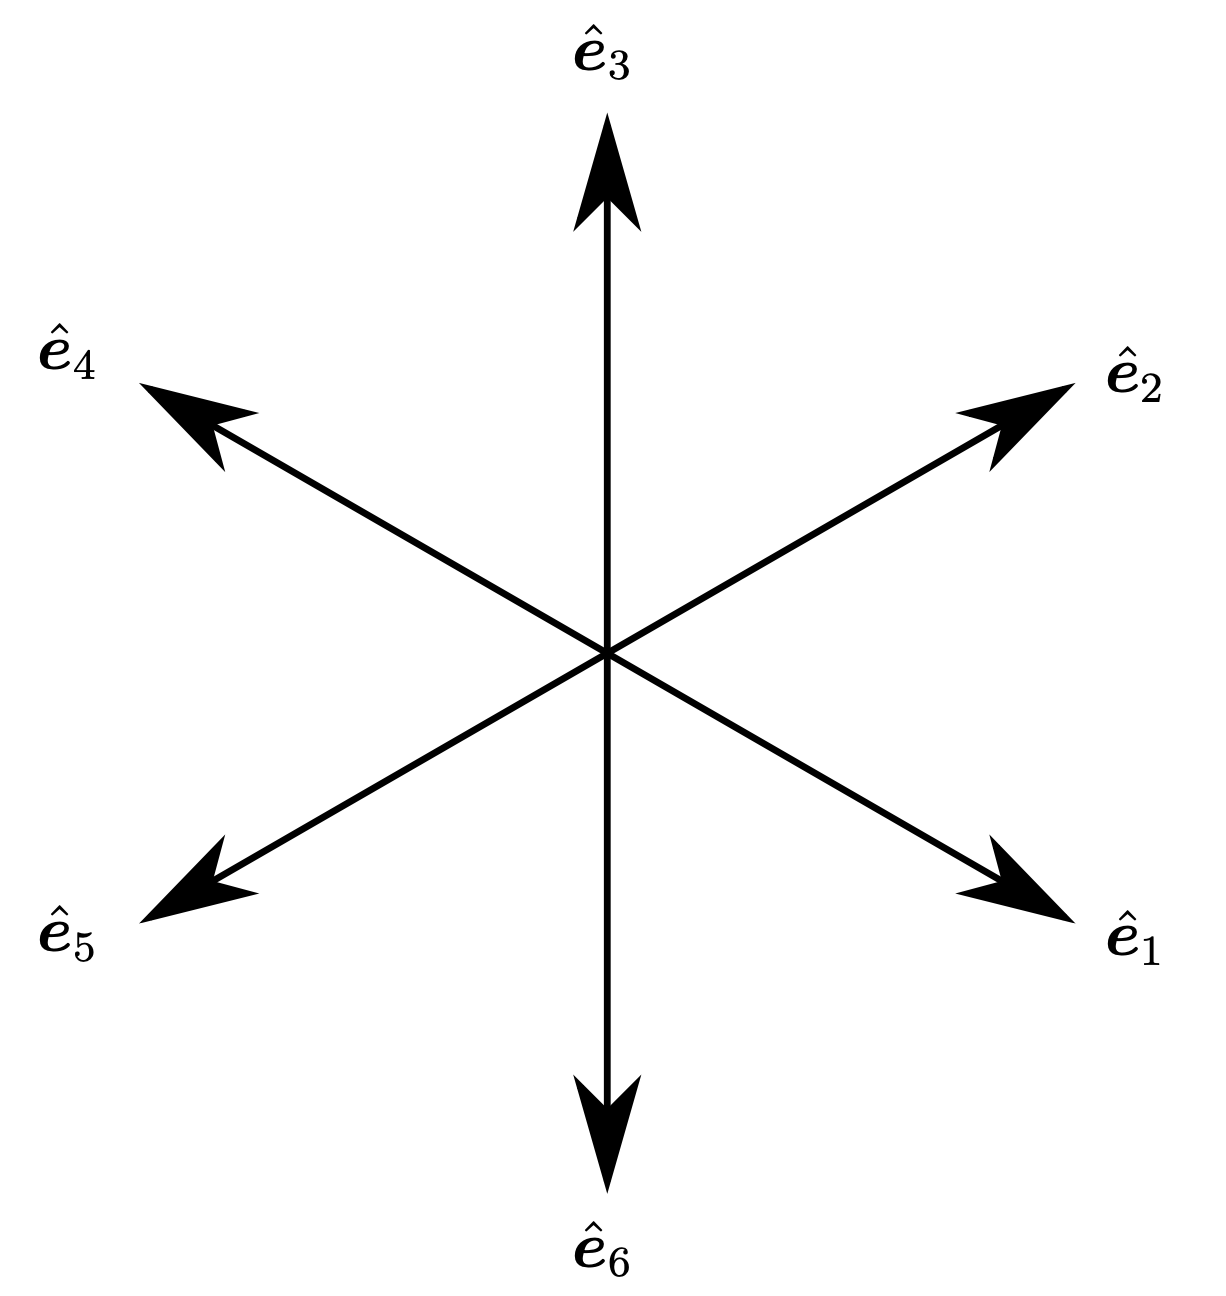
\includegraphics[width=0.5\columnwidth]{figures/LGA_lattice.png}
    \bicaption{二维速度空间中FPH模型的六边形格子,其包含有六个离散速度方向。}{Hexagonial lattice of the FHP model with six discrete velocity directions in two-dimensional velocity space.}
    \label{img:LGA_lattice}
\end{figure}

不论LGA或LBM,有一个通用的假设是,在一个时间步长$\Delta t$后,一个粒子会正好走过两个相邻格点间的距离$\Delta x$。对于一个六边形网格,有
\begin{equation}
    \mathbf{\xi}_i=\frac{\Delta x}{\Delta t}\hat{\mathbf{e}}_i,
\end{equation}
其中$\hat{\mathbf{e}}_i=\mathbf{e}_i/|\mathbf{e}_i|$是正则化后的粒子运动方向,$i$是速度方向的标号,$\mathbf{\xi}_i$是离散速度。那么接下来可以定义粒子的状态$n_{i}(\mathbf{x},t)$,这个状态值可以是0或1。不考虑碰撞的话,粒子的运动可以用方程描述:
\begin{equation}
    n_{i}(\mathbf{x}+\mathbf{\xi}_i \Delta t,t+\Delta t)=n_{i}(\mathbf{x},t).
    \label{eq:LGA}
\end{equation}
公式~\ref{eq:LGA}构成了LGA中标志性的迁移步骤。这一过程也被LBM所继承。这一点为LBM方法带来了很大的优势,首先就是线性的对流项大幅降低了计算难度。其次是这一种直接的空间离散形式并不需要生成一个特殊的计算网格,使前处理的复杂度也能大幅下降。然而这并不代表LBM对网格完全没有要求,这类基于格子的方法只能被应用于六边形或更常见的笛卡尔网格也是一种对网格的约束。

在LGA中,因为粒子只有两种状态,所以经常使用布尔 (Boolean) 变量表示。一般值为真 (true) 时表示在某个空间位置上有一个粒子正在以特定的速度移动,而值为假 (false) 时表示没有这样的粒子。这清楚地显示LGA方法是在粒子层面来表示流体的运动的~\cite{wolf2004lattice}。而很显然,想要完全真实地使用粒子来表示流体是不现实的,因为$1cm^3$的空气中就含有约$2.7\times 10^{19}$个粒子。这导致LGA只能采用比现实情况要低得多的粒子量进行仿真,使结果有很强的噪声。从而方法需要在空间和时间上进行平均才能取得相对正常的结果。为了解决这一问题,McNamara和Zanetti~(\citeyear{mcnamara1988use})提出使用一个表示粒子密度的分布函数来替代这种单个的粒子。这种抽象的表达也是玻尔兹曼输运方程 (Boltzmann Transport Equation, BTE) 的构成基础。所以被传输的值不再只是一个布尔值,而是一个实数。这个实数表达了在空间位置$\mathbf{x}$、时间$t$,找到一个速度为$\mathbf{\xi}$的粒子的概率的空间密度。那么在没有碰撞时的迁移步骤的方程变为:
\begin{equation}
    f_{i}(\mathbf{x}+\mathbf{\xi}_i \Delta t,t+\Delta t)=f_{i}(\mathbf{x},t),
    \label{eq:LBM_streaming}
\end{equation}
其中$f_{i}$是上述的概率分布函数,一般简称为分布函数。一般认为这标志着LBM的诞生。因为在微观过程上使用了统计的概念,所以LBM被称为介观 (mesoscopic) 方法。在公式~\ref{eq:LGA}与~\ref{eq:LBM_streaming}中,粒子间的交互被忽略了。考虑粒子间的交互,这个过程可以表示为
\begin{equation}
    f_{i}(\mathbf{x}+\mathbf{\xi}_i \Delta t,t+\Delta t)=f_{i}(\mathbf{x},t)+\Omega(f_{i}(\mathbf{x},t)),
    \label{eq:LBM_in_one}
\end{equation}
其中$\Omega$是碰撞运算符。然而在实际中,通常会将公式~\ref{eq:LBM_in_one}表示为两个分开的过程,即碰撞和迁移:
\begin{alignat}{2}
\textbf{碰撞:} & \quad\quad &f_i^*(\boldsymbol{x}, t) & =f_i(\boldsymbol{x}, t)+\Omega\left(f_i(\boldsymbol{x}, t)\right); \\
\textbf{迁移:} & & f_i\left(\boldsymbol{x}+\boldsymbol{\xi}_i \Delta t, t+\Delta t\right) & =f_i^*(\boldsymbol{x}, t),\label{eq:LBM_streaming_in_one}
\end{alignat}
其中,$f_i^*$表示碰撞后的分布函数。为了满足质量与动量守恒,LGA中的碰撞中设定了一些固定的规则。对于FHP模型来说,其只允许两个或三个粒子间的碰撞,并且粒子离开格点的方向不能和进入格点的方向一样。这使得两个粒子间的碰撞只有两种可能的结果,而三个粒子间的碰撞只有一种可能的结果,参见图~\ref{img:LGA_collision}。

\begin{figure}[htb]
    \centering
      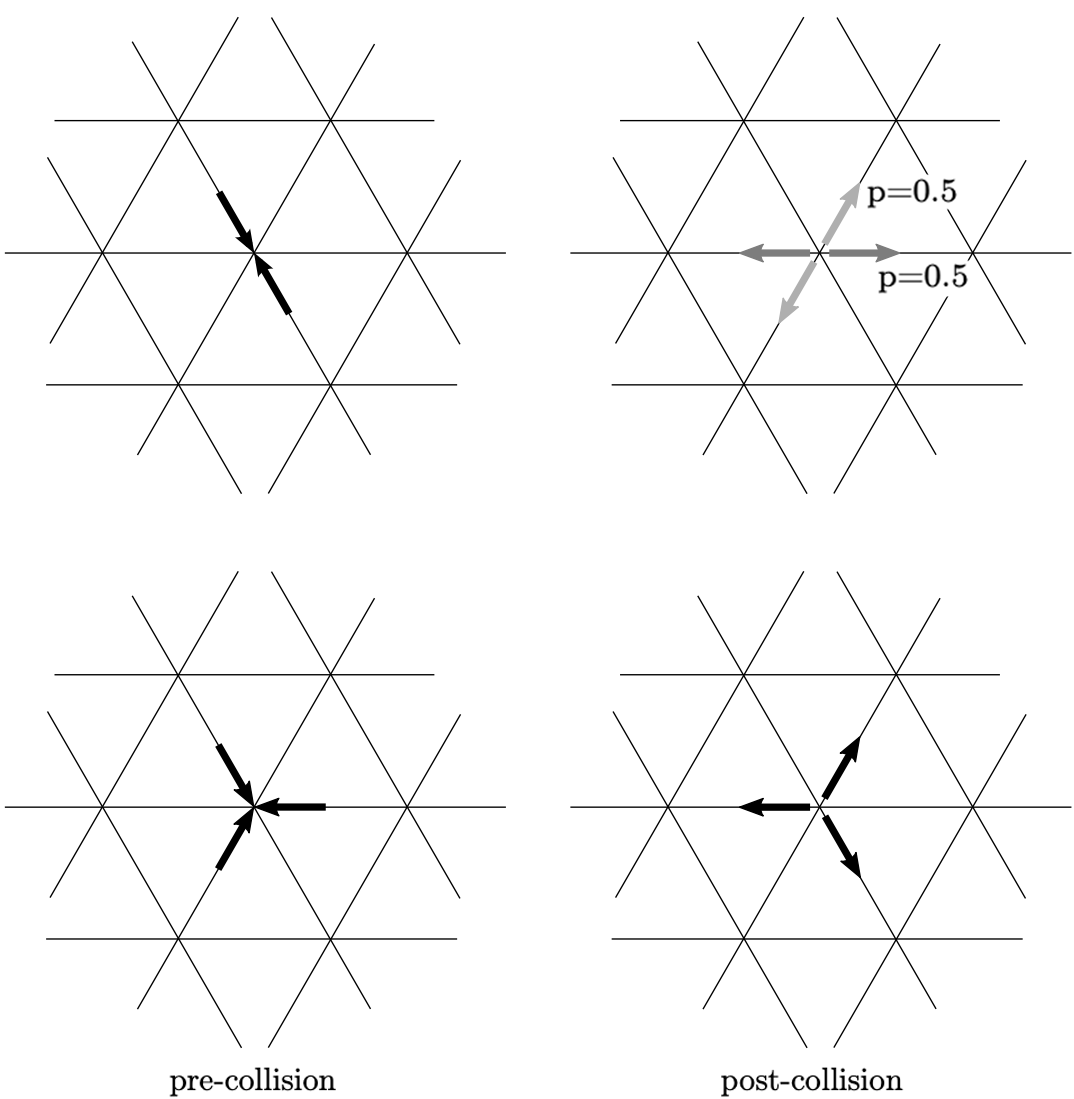
\includegraphics[width=0.9\columnwidth]{figures/LGA_collision.png}
    \bicaption{FHP模型中,两个粒子间的碰撞与三个粒子间的碰撞示意。$p$表示碰撞后的概率分布。}{Two- and three-particle collision in the FHP model. $p$ denotes the probablility of a particular post-collision state.}
    \label{img:LGA_collision}
\end{figure}

虽然,最初的LB模型也是基于这些碰撞规则,但是很快人们发现这样的碰撞规则不仅物理上不够精确,对于三维来说,所需的计算量也是不现实的。于是另一种增强的碰撞方案被提出~\cite{higuera1989lattice, higuera1989boltzmann},该方案将非线性的碰撞运算进行了线性化,使碰撞后的值与一个平衡态产生联系:
\begin{equation}
    \Omega(f_{i}(\mathbf{x}, t))=\mathbf{A}_{\alpha\beta}(f_{i}(\mathbf{x},t)+f_{i}^{eq}(\mathbf{x},t)),
\end{equation}
其中$\mathbf{A}$是一个散射矩阵 (scattering matrix),$f_{i}^{eq}$是离散的麦克斯韦-玻尔兹曼平衡态函数 (Maxwell-Boltzmann equilibrium function)。之后Qian等~(\citeyear{qian1992lattice}) 进一步对碰撞模型的简化,基本确定了现在最常见的LBM的碰撞形式,即粒子间的碰撞可以看作是分布函数向平衡态的一个松弛过程:
\begin{equation}
    \mathbf{A}=-\delta_{\alpha\beta}\tilde{\omega}.
\end{equation}
那么这个散射矩阵事实上可以被一个松弛系数$\tilde{\omega}$替代了,这个系数是松弛时间$\tilde{\tau}$的倒数:$\tilde{\omega}^{-1}=\tilde{\tau}=\frac{\tau}{\Delta t}$. 从而,公式~\ref{eq:LBM_in_one}变为
\begin{equation}
    f_{i}(\mathbf{x}+\mathbf{\xi}_i \Delta t,t+\Delta t)=f_{i}(\mathbf{x},t)-\tilde{\omega}(f_{i}(\mathbf{x},t)-f_{i}^{eq}(\mathbf{x},t)).
    \label{eq:LBM_in_one_BGK}
\end{equation}
现在所有的分布函数都以相同的速率向平衡态松弛,虽然这样非常地简洁高效,但是这种方法没有考虑对于分布函数中有物理意义和没有物理意义的部分是否需要分开处理。之后d'Humières~(\citeyear{d1992generalized}) 证明散射矩阵$\mathbf{A}$可以由一组特征基得到,这为多松弛时间模型的出现奠定了基础。

这种对碰撞本身的效果建模,而不是对微观过程建模的想法,最早可见于连续玻尔兹曼方程中的BGK碰撞模型~\cite{Bhatnagar-1954}。这个想法背后的动机是碰撞过程的大部分细节并不会对宏观量产生影响,所以可以将这些过程省略。除了质量与动量守恒之外,BGK模型还满足$\mathrm{H}$-定理,即分布函数会向平衡态趋近。基于BGK的LBM也是最简洁、最常见的LBM模型。


% Sec 2.2
\section{从介观量到宏观量}
对于大多数的流体应用,使用一组连续的状态量来描述,如速度、压力等一般已经足够。这些量其实是微观粒子状态的统计平均。在宏观上,流体可以被视为连续体并由N-S方程描述。然而LBM并非是一个宏观方法,而是介于微观与宏观之间的介观层面,如图~\ref{img:fluid_abstraction} 所示。

\begin{figure}[htb]
    \centering
      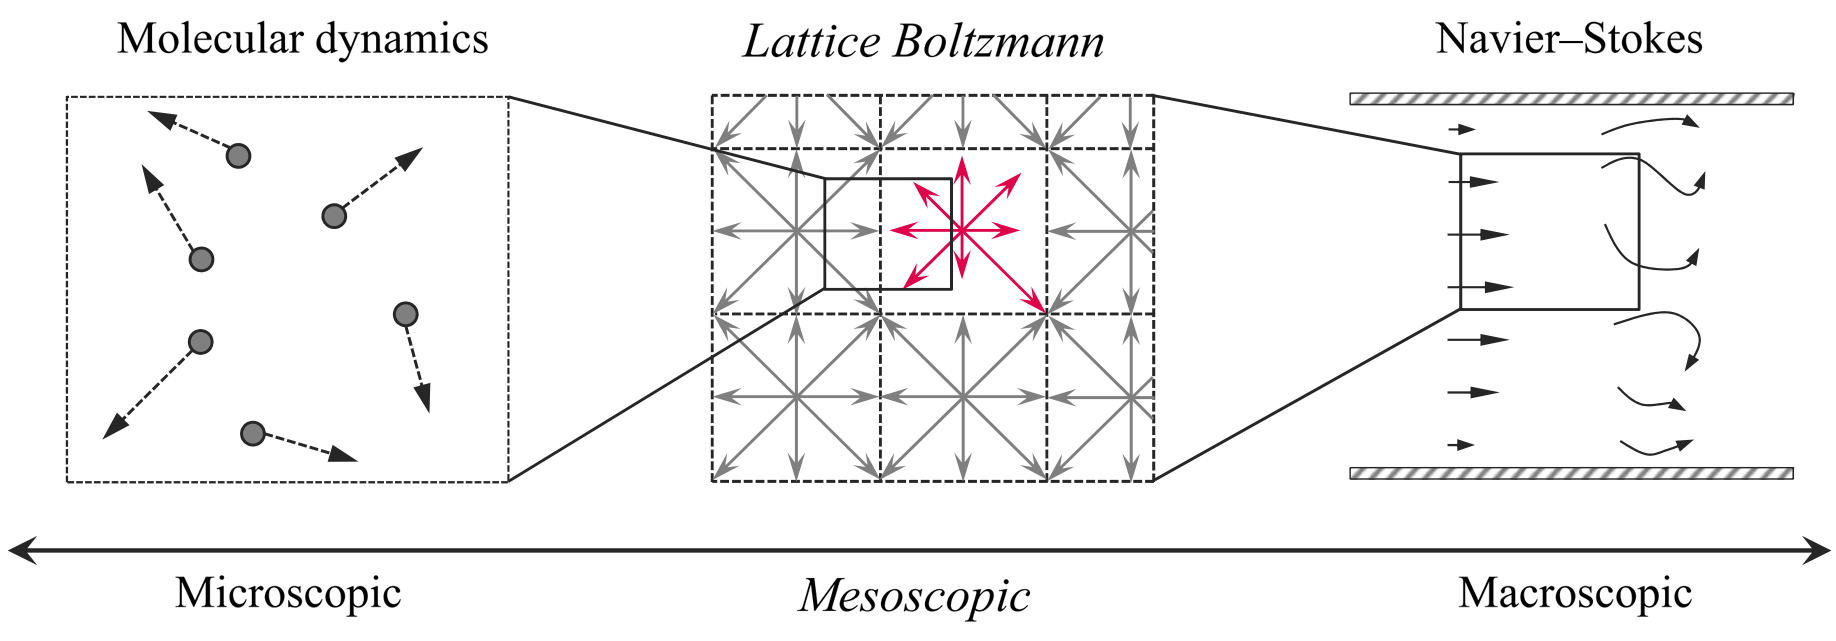
\includegraphics[width=0.9\columnwidth]{figures/fluid_abstraction.png}
    \bicaption{流体力学中的不同抽象层级。}{Different abstraction levels of the fluid dynamics.}
    \label{img:fluid_abstraction}
\end{figure}

可以认为LBM虽然采用了一种非常简化的方案,但它依然计算了部分的微观层面的交互。这也使得LBM的求解过程与N-S方程求解有本质的区别。然而我们最终目的依然是获取宏观的流体状态,以符合我们在宏观世界中对流体的感受。接下来我们将逐步介绍LBM中的概念,并建立其与宏观世界的联系。

可以认为,在一个给定的控制体积 (control volume) 中,分布函数表示了速度在$\boldsymbol{\xi}$与$\boldsymbol{\xi}+d\boldsymbol{\xi}$之间的粒子总数。所以宏观和介观值可以通过对速度空间$\boldsymbol{\Xi}$积分来建立联系,通过积分我们可以得到速度的n阶矩
\begin{equation}
    \boldsymbol{M}^{(n)}=\int_{\mathbb{R}^{\mathrm{D}}} \underbrace{\boldsymbol{\xi} \boldsymbol{\xi} \ldots \boldsymbol{\xi}}_{\mathrm{n} \text {次}} f(\boldsymbol{x}, \boldsymbol{\xi}, t) \mathrm{d} \boldsymbol{\xi},
\end{equation}
这里$D$代表积分的维度。在宏观层面,质量、动量和能量的守恒是由方程自身保证的,然而在介观层面,我们需要通过对碰撞运算符进行约束来保证,这个约束可以写作
\begin{equation}
    \int\left(\Omega(f) \cdot \psi\right) \mathrm{d} \boldsymbol{\xi}=0,
    \label{eq:collision_invariants}
\end{equation}
其中$\psi_k$是碰撞不变量 (collision invariants)。质量、动量和能量的守恒要求当$\psi=1, \boldsymbol{\xi}, |\boldsymbol{\xi}|^2$时,公式~\ref{eq:collision_invariants}是成立的。如果我们将碰撞不变量与分布函数的积进行积分,我们可以自然地得到连续速度空间中的宏观量
\begin{equation}
    \left\{\begin{array}{l}\rho(\boldsymbol{x}, t)=\int f(\boldsymbol{x}, \boldsymbol{\xi}, t) \mathrm{d} \boldsymbol{\xi} \\ \rho \boldsymbol{u}(\boldsymbol{x}, t)=\int \boldsymbol{\xi} f(\boldsymbol{x}, \boldsymbol{\xi}, t) \mathrm{d} \boldsymbol{\xi} \\ \rho E(\boldsymbol{x}, t)=\frac{1}{2} \int|\boldsymbol{\xi}|^2 f(\boldsymbol{x}, \boldsymbol{\xi}, t) \mathrm{d} \boldsymbol{\xi}\end{array}\right.,
\end{equation}
其中$E$为比能量 (specific energy)。对于单原子气体,碰撞可以假设为弹性的,所以比能量包含内能与动能
\begin{equation}
    \rho E=\rho\left(e+\frac{1}{2}|\boldsymbol{u}|^2\right).
\end{equation}
对于本动速度 (peculiar velocity) $\boldsymbol{v}=\boldsymbol{\xi}-\boldsymbol{u}$,即粒子在速度为$\boldsymbol{u}$的平均流中的相对速度,我们可以得到类似的公式:
\begin{equation}
    \rho e(\boldsymbol{x}, t)=\frac{1}{2} \int|\boldsymbol{v}|^2 f(\boldsymbol{x}, \boldsymbol{\xi}, t) \mathrm{d} \boldsymbol{\xi}.
\end{equation}
在连续概念的流体力学中,内能的守恒方程需要通过一个状态方程$p=p(\rho,e)$将压力和密度联系起来,即
\begin{equation}
    p=\frac{1}{\mathrm{D}} \int|\boldsymbol{v}|^2 f(\boldsymbol{x}, \boldsymbol{\xi}, t) \mathrm{d} \boldsymbol{\xi}=\frac{2}{\mathrm{D}} \rho e.
    \label{eq:eos}
\end{equation}
对于满足理想气体定律 (perfect gas law) 的等温流体,可以得到
\begin{equation}
    e=\frac{\mathrm{D}}{2} \frac{p}{\rho}=\frac{\mathrm{D}}{2} R T_0=\frac{\mathrm{D}}{2} \frac{k_B T_0}{m}=\frac{\mathrm{D}}{2} c_s^2,
\end{equation}
其中$T_0$和$c_s$分别表示常值的温度与声速,$k_B$是玻尔兹曼常数,$R$是气体常数。所以公式~\ref{eq:eos}可以被重写为
\begin{equation}
    p=\rho c_s^2,
\end{equation}
即绝热系数$\gamma=1$时的等熵状态方程~\cite{kundu2015fluid}。


% Sec 2.3
\section{速度空间的离散化}
如前文所述,由于在求解时保留了格子的概念,所以我们必须类似地对速度空间进行离散。分布函数事实上可以表达为Hermite多项式构成的无穷级数,变量为经过声速正则化后的速度空间$\tilde{\xi}=\xi/c_s$:
\begin{equation}
    f(\boldsymbol{x}, \boldsymbol{\xi}, t)=\frac{1}{c_s^{\mathrm{D}}} \omega(\tilde{\boldsymbol{\xi}}) \sum_{n=0}^{\infty} \frac{1}{n !} \boldsymbol{a}^{(n)}(\boldsymbol{x}, t) \mathscr{H}^{(n)}(\tilde{\boldsymbol{\xi}}),
    \label{eq:hermite_f}
\end{equation}
其中$\mathscr{H}^{(n)}$是$n$次多项式。Hermite多项式的一个特点是展开系数$\boldsymbol{a}^{(n)}$是$f$本身的速度矩~\cite{shan2006kinetic},权重函数$\omega$为
\begin{equation}
    \omega(\tilde{\boldsymbol{\xi}})=\frac{1}{(2 \pi)^{\mathrm{D} / 2}} \exp \left(-\tilde{\boldsymbol{\xi}}^2 / 2\right).
\end{equation}
当流体不受压力时,流体可以被一个平衡态函数描述。这只会出现在密度和速度在整个流体域中都是常值的情况下。此时的平衡态可由麦克斯韦分布函数描述
\begin{equation}
    f^{eq}=\frac{\rho}{\left(2 \pi c_s^2\right)^{\mathrm{D} / 2}} \exp \left(\frac{-(\boldsymbol{\xi}-\boldsymbol{u})^2}{2 c_s^2}\right),
    \label{eq:maxwell_eq}
\end{equation}
其中$\rho$和$\boldsymbol{u}$分别为宏观的密度和速度。我们可以将这个平衡态函数投影到基为Hermite多项式的空间,此时速度矩变为$\boldsymbol{a}^{eq,(n)}$:
\begin{equation}
    f^{eq}(\boldsymbol{x}, \boldsymbol{\xi}, t)=\frac{1}{c_s^{\mathrm{D}}} \omega(\tilde{\boldsymbol{\xi}}) \sum_{n=0}^{\infty} \frac{1}{n !} \boldsymbol{a}^{eq,(n)}(\boldsymbol{x}, t) \mathscr{H}^{(n)}(\tilde{\boldsymbol{\xi}}).
    \label{eq:maxwell_eq_hermite}
\end{equation}
对比公式~\ref{eq:maxwell_eq},我们可以注意到两式几乎有着相同的形式。事实上,$f^{eq}$还可表达为
\begin{equation}
    f^{eq}=\frac{\rho}{c_s^D}\omega(\tilde{\boldsymbol{v}}),
\end{equation}
其中$\tilde{\boldsymbol{v}}=(\boldsymbol{\xi})$可视为本动马赫数。所以麦克斯韦分布函数的Hermite展开系数为
\begin{equation}
    \boldsymbol{a}^{eq,(n)}=\rho \int w(\tilde{\boldsymbol{v}}) \mathscr{H}^{(n)}\left(\tilde{\boldsymbol{v}}+\frac{\boldsymbol{u}}{c_s}\right) \mathrm{d} \tilde{\boldsymbol{v}}.
    \label{eq:hermite_coefficients}
\end{equation}
对公式~\ref{eq:hermite_f}这样的无穷级数进行截断,即对应着对速度空间的离散化,并且保证了连续空间和离散空间下的矩在截断的阶数前是不变的。而离散的一个重要约束来自于高斯积分
\begin{equation}
    \int w(\boldsymbol{x}) f(\boldsymbol{x}) \mathrm{d} \boldsymbol{x} \approx \sum w_i f(\boldsymbol{x}_i), \quad i=0,1, \ldots, q-1
\end{equation}
其中,$f(\boldsymbol{x})$可表示任意函数而$\omega_i$是常值的权重。
%我们用$\tilde{\xi}_i$表达在$N$阶截断后的Hermite级数的横坐标 (abscissae),则高阶的截断一定会需要更多数量的离散速度,使格子的拓扑更难构造。
我们可以将高斯积分的公式抽象地记为
\begin{equation}
    E^q_{D,n},
\end{equation}
其中$D$表示空间的维度,$n$为积分精度的阶数,$q$表示积分所需要的离散点的数量。则我们可以推导出这三个值间的关系。对于一维空间,约束为$n>2N$并且$n=2q-1$~\cite{shan2006kinetic},所以可得$q=N+1$。对于高维空间并没有一般的高斯积分理论,但是我们可以假设有
\begin{equation}
    q=(N+1)^D.
\end{equation}
则二维的速度空间在$N=2$阶截断时需要9个离散速度,$N=3$时需要16个。当然实际的格子方向可能有所不同,因为考虑到某些矩的对称性,在维持$N$不变时所需的离散速度数量可能会减少。然而从几何上考虑,要设计能充满空间且各向同性的格子可能又会增加所需的格子方向数量。如果依然采用~\cite{qian1992lattice}中的D$d$Q$q$的命名的话,能维持二阶精度的格子分别为D1Q3、D2Q9、D3Q16。由公式~\ref{eq:hermite_coefficients}可得,在截断至二阶时,Hermite展开的系数为
\begin{equation}
    \left\{\begin{array}{l}\boldsymbol{a}^{eq, 0}=\rho \\ \boldsymbol{a}^{eq, 1}=\rho \frac{\boldsymbol{u}}{c_s} \\ \boldsymbol{a}^{eq, 2}=\rho \frac{u_i u_j}{c_s^2}\end{array}\right.
\end{equation}
将其代入到公式~\ref{eq:maxwell_eq_hermite}中,可以得到
\begin{equation}
    f_i^{eq}(\boldsymbol{x}, t)=w_i \rho\left(1+\frac{\boldsymbol{\xi}_i \cdot \boldsymbol{u}}{c_s^2}+\frac{\left(\boldsymbol{\xi}_i \cdot \boldsymbol{u}\right)^2}{2 c_s^4}-\frac{u^2}{2 c_s^2}\right),
    \label{eq:f_eq_o2}
\end{equation}
其中$f_i^{eq}(\boldsymbol{x}, t)=f^{eq}(\boldsymbol{x}, \xi_i, t)$, $\omega_i=\omega(\frac{\xi}{c_s})/c_s^D$。上述的推导尝试在尽量保持简洁的前提下,用比较系统且严格的形式推导出分布函数及速度空间的离散,所以无法过于详尽地展示出所有步骤。对于更彻底的推导,读者们可以参考~\cite{shan2006kinetic, malaspinas2010lattice}。


% Sec 2.4
\section{从LBM到N-S方程}
在介绍过速度矩作为介观和宏观世界之间的联系之后,我们现在将使用多尺度分析 (Multiple-scale Analysis) 来从LBE推导出N-S方程。许多流体的动态特征其实表现于其与平衡态的偏移。如果在介观上,分布函数都处于平衡态,那么可以想像,在宏观上流体也是平静的。所以多尺度分析的思想是将$f$在$f^{eq}$处展开。展开后的$f^{eq}$可以被记为$f^{(0)}$,其余部分为非平衡态项:
\begin{equation}
    f=\underbrace{f^{(0)}}_{f^{e q}}+\underbrace{\epsilon f^{(1)}+\epsilon^2 f^{(2)}}_{f^{n e q}} \cdots .
\end{equation}
多尺度分析的扩展依赖于一个很小的参数$\epsilon$,这个值是碰撞时间$\tau=\nu/c_s^2$与格子时间步长$\Delta t$的比值。对流的时间尺度 (advection timescale) 是直接与$\Delta t_1=\tau/\epsilon$联系的,而粘性扩散的时间尺度 ( viscous diffusion timescale) 是联系于
\begin{equation}
    \Delta t_2=\frac{\Delta x^2}{\nu} \sim \frac{c_s^2 \Delta t^2}{\nu}=\frac{\tau}{\epsilon^2}
    \label{eq:ms_f}
\end{equation}
的。有推导证明我们将$f$展开到一阶 ($\epsilon f^{(1)}$) 时,可以推导出欧拉方程~\cite{huang2008statistical}。为了推导N-S方程,我们需要展开到二阶 (即$\epsilon^2 f^{(2)}$),此时时间上的导数运算符为
\begin{equation}
    \frac{\partial}{\partial t}=\epsilon \frac{\partial}{\partial t_1}+\epsilon^2 \frac{\partial}{\partial t_2},
    \label{eq:ms_t}
\end{equation}
空间上的导数运算符为
\begin{equation}
    \frac{\partial}{\partial \boldsymbol{x}}=\epsilon \frac{\partial}{\partial \boldsymbol{x}_1}.
    \label{eq:ms_x}
\end{equation}
在将$f$分解为平衡态与非平衡态后,公式~\ref{eq:collision_invariants}所表达的约束可被表达为
\begin{equation}
    \sum_{i} f_{i}^{(n)}=\sum_{i} \boldsymbol{\xi}_{i} f_{i}^{(n)}=0, \quad  n=1,2, \ldots.
\end{equation}
那么为了将LBE恢复到N-S方程,首先我们要将公式~\ref{eq:LBM_in_one_BGK}的左手侧进行二阶的泰勒展开
\begin{align}
    \begin{split}
        & f_{i}\left(\boldsymbol{x}+\boldsymbol{\xi}_{i} \Delta t, t+\Delta t\right) \approx \\
        & \quad f_{i}(\boldsymbol{x}, t)+\left(\xi_{i \alpha} \Delta t \frac{\partial}{\partial x_{\alpha}}+\Delta t \frac{\partial}{\partial t}\right) f_{i}(\boldsymbol{x}, t)+ \\
        & \quad \frac{1}{2}\left(\xi_{i \alpha} \xi_{i \beta} \Delta t^{2} \frac{\partial^{2}}{\partial x_{\alpha} \partial x_{\beta}}+2 \xi_{i \alpha} \Delta t^{2} \frac{\partial}{\partial x_{\alpha}} \frac{\partial}{\partial t}+\Delta t^{2} \frac{\partial^{2}}{\partial t^{2}}\right) f_{i}(\boldsymbol{x}, t)+\mathcal{O}\left(\Delta t^{3}\right) .
    \end{split}
    \label{eq:ms_taylor}
\end{align}
我们将上式代入公式~\ref{eq:LBM_in_one_BGK},并用$\tau$替代$\tilde{\omega}$后,可以得到
\begin{equation}
\Delta t\left(\xi_{i \alpha} \frac{\partial}{\partial x_{\alpha}}+\frac{\partial}{\partial t}\right) f_{i}+\frac{\Delta t^{2}}{2}\left(\xi_{i \alpha} \xi_{i \beta} \frac{\partial^{2}}{\partial x_{\alpha} \partial x_{\beta}}+2 \xi_{i \alpha} \frac{\partial}{\partial x_{\alpha}} \frac{\partial}{\partial t}+\frac{\partial^{2}}{\partial t^{2}}\right) f_{i}=-\frac{\Delta t}{\tau}\left(f_{i}-f_{i}^{e q}\right) .
\end{equation}
接下来,我们将多尺度分析的公式~\ref{eq:ms_f}至~\ref{eq:ms_x}代入上式
\begin{align}
    \begin{split}
& {\left[\xi_{i \alpha}\left(\epsilon \frac{\partial}{\partial x_{1 \alpha}}\right)+\left(\epsilon \frac{\partial}{\partial t_{1}}+\epsilon^{2} \frac{\partial}{\partial t_{2}}\right)\right]\left(f_{i}^{(0)}+\epsilon f_{i}^{(1)}+\epsilon^{2} f_{i}^{(2)}\right)+} \\
& \frac{\Delta t}{2}\left[\xi_{i \alpha} \xi_{i \beta}\left(\epsilon^{2} \frac{\partial^{2}}{\partial x_{1 \alpha} \partial x_{1 \beta}}\right)+\left(2 \xi_{i \alpha} \epsilon^{2} \frac{\partial}{\partial x_{1 \alpha}} \frac{\partial}{\partial t_{1}}\right)+\left(\epsilon^{2} \frac{\partial^{2}}{\partial t_{1}^{2}}\right)\right]\left(f_{i}^{(0)}+\epsilon f_{i}^{(1)}+\epsilon^{2} f_{i}^{(2)}\right)= \\
& \quad-\frac{1}{\tau}\left(f_{i}^{(0)}+\epsilon f_{i}^{(1)}+\epsilon^{2} f_{i}^{(2)}-f_{i}^{e q}\right) .
    \end{split}
    \label{eq:ms_total}
\end{align}
接下来,我们把公式~\ref{eq:ms_total}按照$\epsilon$的阶数分离:

\noindent
$\mathcal{O}\left(\epsilon^{0}\right):$
\begin{equation}
f_{i}^{(0)}=f_{i}^{e q}
\end{equation}
$\mathcal{O}\left(\epsilon^{1}\right):$
\begin{equation}
\epsilon\left(\xi_{i \alpha} \frac{\partial}{\partial x_{1 \alpha}}+\frac{\partial}{\partial t_{1}}\right) f_{i}^{(0)}=-\frac{1}{\tau} \epsilon f_{i}^{(1)}
\label{eq:ms_o1}
\end{equation}
$\mathcal{O}\left(\epsilon^{2}\right):$
\begin{equation}
\epsilon^{2} \frac{\partial}{\partial t_{2}} f_{i}^{(0)}+\left(\xi_{i \alpha} \epsilon \frac{\partial}{\partial x_{1 \alpha}}+\epsilon \frac{\partial}{\partial t_{1}}\right) \epsilon f_{i}^{(1)}+\frac{\Delta t}{2}\left(\xi_{i \alpha} \epsilon \frac{\partial}{\partial x_{1 \alpha}}+\epsilon \frac{\partial}{\partial t_{1}}\right)^{2} f_{i}^{(0)}=-\frac{1}{\tau} \epsilon^{2} f_{i}^{(2)}
\label{eq:ms_o2}
\end{equation}
将公式~\ref{eq:ms_o1}代入公式~\ref{eq:ms_o2},可以得到
\begin{equation}
\epsilon^{2} \frac{\partial}{\partial t_{2}} f_{i}^{(0)}+\left(\xi_{i \alpha} \epsilon \frac{\partial}{\partial x_{1 \alpha}}+\epsilon \frac{\partial}{\partial t_{1}}\right)\left(1-\frac{\Delta t}{2 \tau}\right) \epsilon f_{i}^{(1)}=-\frac{1}{\tau} \epsilon^{2} f_{i}^{(2)}
\label{eq:ms_o1_into_o2}
\end{equation}
接下来我们想要获得关于宏观量的守恒公式,与求矩类似,我们对公式~\ref{eq:ms_o1}与公式~\ref{eq:ms_o1_into_o2}对碰撞不变量积分得到0阶与1阶的矩公式
\begin{equation}
\epsilon \frac{\partial \rho}{\partial t_{1}}+\epsilon \frac{\partial \rho u_{\alpha}}{\partial x_{1 \alpha}}=0,
\label{eq:ms_moment_o1_a}
\end{equation}
\begin{equation}
\epsilon \frac{\partial \rho u_{\alpha}}{\partial t_{1}}+\epsilon \frac{\partial P_{\alpha \beta}^{(0)}}{\partial x_{1 \beta}}=0,
\label{eq:ms_moment_o1_b}
\end{equation}
同样地,我们对公式~\ref{eq:ms_o2}积分得到矩公式
\begin{equation}
\epsilon^{2} \frac{\partial \rho}{\partial t_{2}} = 0,
\label{eq:ms_moment_o2_a}
\end{equation}
\begin{equation}
\epsilon^{2} \frac{\partial \rho u_{\alpha}}{\partial t_{2}} +\left(1-\frac{\Delta t}{2 \tau}\right) \epsilon^{2} \frac{P_{\alpha \beta}^{(1)}}{\partial x_{1 \beta}}=0 .
\label{eq:ms_moment_o2_b}
\end{equation}
然后我们将公式~\ref{eq:ms_moment_o1_a}与~\ref{eq:ms_moment_o1_b}相加,并将展开的求导运算符重新代回原式 (参见公式~\ref{eq:ms_t}与~\ref{eq:ms_x}) 可以得到
\begin{equation}
\frac{\partial \rho}{\partial t}+\frac{\partial \rho u_{\alpha}}{\partial x_{\alpha}}=0,
\end{equation}
即连续性方程。同样将公式~\ref{eq:ms_moment_o2_a}与~\ref{eq:ms_moment_o2_b}相加后得到
\begin{equation}
\frac{\partial \rho u_{\alpha}}{\partial t}+\frac{\partial}{\partial x_{\beta}}\left[P_{\alpha \beta}^{e q}+\left(1-\frac{\Delta t}{2 \tau}\right) P_{\alpha \beta}^{n e q}\right]=0,
\label{eq:ms_continuity_puzzle}
\end{equation}
其中$P_{\alpha \beta}^{e q}=P_{\alpha \beta}^{(0)}$,$P_{\alpha \beta}^{n e q}=P_{\alpha \beta}^{(1)}$。
由公式~\ref{eq:f_eq_o2}我们可以由下面的方式得到二阶矩
\begin{equation}
P_{\alpha \beta}^{(0)}=P_{\alpha \beta}^{e q}=\sum_{\alpha} f_{i}^{e q} \xi_{i, \alpha} \xi_{i, \beta}=\rho c_{s}^{2}\delta_{\alpha \beta}+\rho u_{\alpha} u_{\beta}.
\end{equation}
与三阶矩
\begin{equation}
Q_{\alpha \beta \gamma}^{(0)}=Q_{\alpha \beta \gamma}^{e q}=\sum_{\alpha} f_{i}^{e q} \xi_{i, \alpha} \xi_{i, \beta} \xi_{i, \gamma}=\rho c_{s}^{2}\left(u_{\alpha} \delta_{\beta \gamma}+u_{\beta} \delta_{\alpha \gamma}+u_{\gamma} \delta_{\alpha \beta}\right).
\end{equation}
那么在公式~\ref{eq:ms_continuity_puzzle}中,只剩下$P_{\alpha \beta}^{n e q}$是未知的。为了计算$P_{\alpha \beta}^{n e q}$,我们写出公式~\ref{eq:ms_o1}的2阶矩公式
\begin{equation}
\epsilon \frac{\partial P_{\alpha \beta}^{(0)}}{\partial t_{1}}+\epsilon \frac{\partial Q_{\alpha \beta \gamma}^{(0)}}{\partial x_{1 \gamma}}=-\frac{1}{\tau} \epsilon P_{\alpha \beta}^{(1)}.
\label{eq:ms_moment_o2}
\end{equation}
接下来,我们引入如下的积分公式 (乘积法则):
\begin{align}
\epsilon \frac{\partial \rho u_{\alpha} u_{\beta}}{\partial t_{1}} & =u_{\alpha} \epsilon \frac{\rho u_{\beta}}{\partial t_{1}}+u_{\beta} \epsilon \frac{\rho u_{\alpha}}{\partial t_{1}}-u_{\alpha} u_{\beta} \epsilon \frac{\partial \rho}{\partial t_{1}}, \\
\epsilon \frac{\partial \rho u_{\alpha} u_{\beta} u_{\gamma}}{\partial x_{1 \gamma}} & =u_{\alpha} \epsilon \frac{\rho u_{\beta} u_{\gamma}}{\partial x_{1 \gamma}}+u_{\beta} \epsilon \frac{\rho u_{\alpha} u_{\gamma}}{\partial x_{1 \gamma}}-u_{\alpha} u_{\beta} \epsilon \frac{\partial \rho u_{\gamma}}{\partial x_{1 \gamma}} .
\end{align}
使用上述的公式,公式~\ref{eq:ms_moment_o2}左手边的$\epsilon \frac{\partial P_{\alpha \beta}^{(0)}}{\partial t_{1}}$可以被表达为
\begin{align}
    \begin{split}
\epsilon \frac{\partial P_{\alpha \beta}^{(0)}}{\partial t_{1}}= & \epsilon \frac{\partial \rho u_{\alpha} u_{\beta}}{\partial t_{1}}+c_{s}^{2} \delta_{\alpha \beta} \epsilon \frac{\partial \rho}{\partial t_{1}} \\
= & u_{\alpha} \epsilon \frac{\partial \rho u_{\beta}}{\partial t_{1}}+u_{\beta} \epsilon \frac{\partial \rho u_{\alpha}}{\partial t_{1}}-u_{\alpha} u_{\beta} \epsilon \frac{\partial \rho}{\partial t_{1}}+c_{s}^{2} \delta_{\alpha \beta} \epsilon \frac{\partial \rho}{\partial t_{1}} \\
= & -u_{\alpha} \epsilon \frac{\partial P_{\beta \gamma}^{(0)}}{\partial x_{1 \gamma}}-u_{\beta} \epsilon \frac{\partial P_{\alpha \gamma}^{(0)}}{\partial x_{1 \gamma}}+u_{\alpha} u_{\beta} \epsilon \frac{\partial \rho u_{\gamma}}{\partial x_{1 \gamma}}-c_{s}^{2} \delta_{\alpha \beta} \epsilon \frac{\partial \rho u_{\gamma}}{\partial x_{1 \gamma}} \quad \text {(由公式~\ref{eq:ms_moment_o1_a}、\ref{eq:ms_moment_o1_b})} \\
= & -u_{\alpha} \epsilon \frac{\partial}{\partial x_{1 \gamma}}\left(\rho u_{\beta} u_{\gamma}+\rho c_{s}^{2} \delta_{\beta \gamma}\right)-u_{\beta} \epsilon \frac{\partial}{\partial x_{1 \gamma}}\left(\rho u_{\alpha} u_{\gamma}+\rho c_{s}^{2} \delta{\alpha \gamma}\right) \\
& +u_{\alpha} u_{\beta} \epsilon \frac{\partial \rho u_{\gamma}}{\partial x_{1 \gamma}}-c_{s}^{2} \delta_{\alpha \beta} \frac{\partial \rho u_{\gamma}}{\partial x_{1 \gamma}} \\
= & -\epsilon \frac{\partial \rho u_{\alpha} u_{\beta} u_{\gamma}}{\partial x_{1 \gamma}}-c_{s}^{2}\left(u_{\alpha} \epsilon \frac{\partial \rho}{\partial x_{1 \beta}}+u_{\beta} \epsilon \frac{\partial \rho}{\partial x_{1 \alpha}}\right)-c_{s}^{2} \delta_{\alpha \beta} \epsilon \frac{\partial \rho u_{\gamma}}{\partial x_{1 \gamma}} .
    \end{split}
\end{align}
同时,$\epsilon \frac{\partial Q_{\alpha \beta \gamma}^{(0)}}{\partial x_{1 \gamma}}$可表达为
\begin{align}
    \begin{split}
\epsilon \frac{\partial Q_{\alpha \beta \gamma}^{(0)}}{\partial x_{1 \gamma}} & =\epsilon \frac{\partial}{\partial x_{1 \gamma}} \rho c_{s}^{2}\left(u_{\alpha} \delta_{\beta \gamma}+u_{\beta} \delta{\alpha \gamma}+u_{\gamma} \delta_{\alpha \beta}\right) \\
& =c_{s}^{2}\left(\epsilon \frac{\partial \rho u_{\alpha}}{\partial x_{1 \beta}}+\epsilon \frac{\partial \rho u_{\beta}}{\partial x_{1 \alpha}}\right)+c_{s}^{2} \delta_{\alpha \beta} \epsilon \frac{\partial \rho u_{\gamma}}{\partial x_{1 \gamma}}.
    \end{split}
\end{align}
将上述两公式相加可得到$P_{\alpha \beta}^{(1)}$的表达式
\begin{equation}
\epsilon P_{\alpha \beta}^{(1)}=-\rho c_{s}^{2} \tau\left(\epsilon \frac{\partial u_{\alpha}}{\partial x_{1 \beta}}+\epsilon \frac{\partial u_{\beta}}{\partial x_{1 \alpha}}\right)+\tau \epsilon \frac{\partial \rho u_{\alpha} u_{\beta} u_{\gamma}}{\partial x_{1 \gamma}}.
\end{equation}
将 $P^{n e q}=\epsilon P^{(1)}$,$\partial / \partial \boldsymbol{x}=\epsilon \partial / \partial \boldsymbol{x}_{1}$代入,我们可以获得
\begin{equation}
P_{\alpha \beta}^{n e q}=\underbrace{-\rho c_{s}^{2} \tau\left(\frac{\partial u_{\alpha}}{\partial x_{\beta}}+\frac{\partial u_{\beta}}{\partial x_{\alpha}}\right)}_{\boldsymbol{\sigma}^{\prime}}+\underbrace{\tau \frac{\partial \rho u_{\alpha} u_{\beta} u_{\gamma}}{\partial x_{k}}}_{\text {误差项}} .
\label{eq:p_neq}
\end{equation}
从上式中我们可以发现,第一项对应于N-S方程中的粘性应力张量 (viscous stress tensor),第二项是误差项,因为平衡态函数$f_i^{eq}$只展开到了二阶,所以$\mathcal{O}\left(u^{3}\right)$项是不正确的。当我们仔细观察公式~\ref{eq:p_neq}时,我们发现当${u_x}^{2} \ll c_{s}^{2}$时,$\mathcal{O}\left(u^{3}\right)$项的模值相比前一项就可以被忽略了。所以在低马赫数时,我们可以直接忽略上式中的误差项。这也是为什么许多工作描述LBM只在弱可压情况下有效。
那么我们将忽略误差项的公式~\ref{eq:p_neq}代入公式~\ref{eq:ms_continuity_puzzle}后,可以得到动量守恒方程
\begin{equation}
    \frac{\partial \rho u_{\alpha}}{\partial t}+\frac{\partial \rho u_{\alpha} u_{\beta}}{\partial x_{\beta}}=-\frac{\partial p}{\partial x_{\alpha}}+\mu \frac{\partial}{\partial x_{\beta}}\left(\frac{\partial u_{\alpha}}{\partial x_{\beta}}+\frac{\partial u_{\beta}}{\partial x_{\alpha}}\right),
\end{equation}
其中$\mu=\left(1-\frac{\Delta t}{2 \tau}\right) \rho c_{s}^{2} \tau$是动力黏度 (dynamic viscosity),运动黏度 (kinematic viscosity) $\nu=\mu / \rho$与松弛时间$\tau$之间的关系为
\begin{equation}
    \nu=c_{s}^{2}\left(\tau-\frac{\Delta t}{2}\right) \quad \text {或} \quad \tau=\frac{\nu}{c_{s}^{2}}+\frac{\Delta t}{2} .
\end{equation}
因为我们在公式~\ref{eq:ms_taylor} 中对LBE进行了二阶的泰勒展开,所以我们认为在时间和空间上LBM可以以二阶的精度推导出N-S方程。


% Sec 2.5
\section{累积量碰撞模型}
在第~\ref{sec:2_LBM_origin} 节的末尾,我们介绍了LBM中的BGK碰撞模型 (即单松弛时间模型) 与多松弛时间模型出现的动机,并在第~\ref{sec:1_related_works_LBM} 节中介绍了基于不同量的MRT模型。在这些碰撞模型中,累积量碰撞模型相比其它模型 (原始矩、中心矩等) 有着遵守伽利略不变性、自由度耦合程度低、超黏度 (hyper-viscosity) 误差更小的优势,所以我们将基于累积量碰撞模型进行改进。在这里我们先简要的介绍累积量碰撞模型本身。

不同的碰撞模型的本质是在探索什么量可以最优地描述分布函数,我们称这些量为可观察量 (observable variables)。在累积量方法中,不同累积量之间是统计独立的 (statistically independent),也就是说,两个累积量的联合概率等于各自概率的积。为了推导出累积量,我们先将分布函数$f$转换到频率空间$F$中,这样便于我们进行泰勒展开。到频域的变换由拉普拉斯变换 (Laplace transform) 完成:
$$
F(\boldsymbol{\Xi})=\mathcal{L}\{f(\boldsymbol{\xi})\}.
$$
在三维中,我们令$\boldsymbol{\Xi}=\{\Xi, \Upsilon, \mathrm{Z}\}$,$\boldsymbol{\Xi}$代表了频率 (波数)。如果我们假设存在一个这样的可观察量$k_{\alpha\beta\gamma}$,使得它们的联合概率是它们各自概率的积
$$
F(\boldsymbol{\Xi})=\prod F_{\alpha \beta \gamma}\left(k_{\alpha \beta \gamma}\right).
$$
为了进行泰勒展开,我们对两边求对数,使等式右手边的积转为和
$$
\ln (F(\boldsymbol{\Xi}))=\sum \ln \left(F_{\alpha \beta \gamma}\left(k_{\alpha \beta \gamma}\right)\right),
$$
则函数$F$的变量$k_{\alpha \beta \gamma}$可被定义为累积量
$$
k_{\alpha \beta \gamma}=\left. \frac{\partial^{\alpha} \partial^{\beta} \partial^{\gamma}}{\partial \Xi^{\alpha} \partial \Upsilon^{\beta} \partial \mathrm{Z}^{\gamma}} \ln (F(\Xi, \Upsilon, \mathrm{Z}))\right|_{\Xi=\Upsilon=\mathrm{Z}=0}.
$$
我们称$k_{\alpha \beta \gamma}$是一个$n=\alpha+\beta+\gamma$阶的累积量。由上述推导,不同累积量是统计无关的,所以它们可以有各自不同的松弛系数
$$
k_{\alpha \beta \gamma}^{*}=\tilde{\omega}_{\alpha \beta \gamma} k_{\alpha \beta \gamma}^{e q}+\left(1-\tilde{\omega}_{\alpha \beta \gamma}\right) k_{\alpha \beta \gamma},
$$
其中$k_{\alpha \beta \gamma}^{*}$与$k_{\alpha \beta \gamma}^{eq}$分别表示碰撞后与平衡态的累积量。在这之后碰撞后的分布函数$f^*$可以由$k_{\alpha \beta \gamma}^{*}$得到。

接下来我们对于D3Q27格子的累积量LBM碰撞模型具体推导。在具体实现时,累积量碰撞过程可以分为五个阶段。第一个阶段是“前向中心矩变换”。虽然通过因为累积量的定义可以进行直接$f$到$k$的变换,但是这个计算过于复杂,而通过中心矩作为中间步骤计算累积量更为简单、有效,所以在实现中会先将$f$变换到中心矩$m$:
$$
m_{\alpha \beta \gamma} =\sum_{i,j,k} (i-u_x)^{\alpha} (j-u_y)^{\alpha} (k-u_z)^{\alpha} f_{ijk},
$$
其中$i, j, k \in \{-1, 0, 1\}$表示离散速度的方向,$\alpha, \beta, \gamma \in \{0, 1, 2\}$表示不同维度的阶数,$\boldsymbol{u}=\{u_x, u_y, u_z\}$表示宏观速度。因为中心矩变换是线性的,所以这个变换其实可以用一个矩阵$M$表示,则反向的变换可以用$M^{-1}$表示。但是我们注意到采用~\cite{Geier-2015}中的分方向的做法可以减少相当部分的计算量:
\begin{align*}
m_{i j \mid \gamma} & =\sum_{k} f_{ijk}(k-u_z)^{\gamma}, \\
m_{i \mid \beta \gamma} & =\sum_{j} m_{i j \mid \gamma}(j-u_y)^{\beta}, \\
m_{\alpha \beta \gamma} & =\sum_{i} m_{i \mid \beta \gamma}(i-u_x)^{\alpha}.
\end{align*}

得到中心矩后,第二个阶段为“前向累积量变换”。对于3阶及以下的累积量,其和中心矩相同:
\begin{align*}
& k_{110}=m_{110}, \\
& k_{200}=m_{200}, \\
& k_{120}=m_{120}, \\
& k_{111}=m_{111} .
\end{align*}
对于$k_{101}$与$k_{020}$等同阶的累积量,可以将上述的对应公式的变量下标交换位置得到。4阶及以上的累积量可通过如下公式得到:
\begin{align*}
k_{211} & =m_{211}-\left(m_{200} m_{011}+2 m_{110} m_{101}\right) / \rho \\
k_{220} & =m_{220}-\left(m_{200} m_{020}+2 m_{110}^{2}\right) / \rho \\
k_{122} & =m_{122}-\left(m_{002} m_{120}+m_{020} m_{102}+4 m_{011} m_{111}+2\left(m_{101} m_{021}+m_{110} m_{012}\right)\right) / \rho \\
k_{222} & =m_{222}-\left(4 m_{111}^{2}+m_{200} m_{022}+m_{020} m_{202}+m_{002} m_{220}\right. \\
&\quad +4\left(m_{011} m_{211}+m_{101} m_{121}+m_{110} m_{112}\right) \\
&\quad \left.+2\left(m_{120} m_{102}+m_{210} m_{012}+m_{201} m_{021}\right)\right) / \rho \\
&\quad +\left(16 m_{110} m_{101} m_{011}+4\left(m_{101}^{2} m_{020}+m_{011}^{2} m_{200}+m_{110}^{2} m_{002}\right)\right. \\
&\quad \left.+2 m_{200} m_{020} m_{002}\right) / \rho^{2} ,
\end{align*}
对于同阶的累积量,同样可以将上述的对应公式的变量下标交换位置得到。

第三个阶段是“碰撞”。首先二阶累积量的碰撞公式如下:
\begin{align*}
& k_{110}^{*}=\left(1-\omega_{1}\right) k_{110}, \\
& k_{101}^{*}=\left(1-\omega_{1}\right) k_{101}, \\
& k_{011}^{*}=\left(1-\omega_{1}\right) k_{011} ,
\end{align*}
其中含星号的变量代表碰撞后的变量。这些累积量的平衡态为0,所以被省去。而由于格子离散化时的各向异性,有些累积量并不为0:
\begin{align*}
k_{200}^{*}-k_{020}^{*} & =\left(1-\omega_{1}\right)\left(k_{200}-k_{020}\right)-3 \rho\left(1-\frac{\omega_{1}}{2}\right)\left({u_x}^{2} \frac{\partial u_x}{\partial x}-{u_y}^{2} \frac{\partial u_y}{\partial y}\right), \\
k_{200}^{*}-k_{002}^{*} & =\left(1-\omega_{1}\right)\left(k_{200}-k_{002}\right)-3 \rho\left(1-\frac{\omega_{1}}{2}\right)\left({u_x}^{2} \frac{\partial u_x}{\partial x}-{u_z}^{2} \frac{\partial u_z}{\partial z}\right), \\
k_{200}^{*}+k_{020}^{*}+k_{002}^{*} & =\kappa_{000} \omega_{2}+\left(1-\omega_{2}\right)\left(k_{200}+k_{020}+k_{002}\right) \\
&\quad -3 \rho\left(1-\frac{\omega_{2}}{2}\right)\left({u_x}^{2} \frac{\partial u_x}{\partial x}+{u_y}^{2} \frac{\partial u_y}{\partial y}+{u_z}^{2} \frac{\partial u_z}{\partial z}\right) ,
\end{align*}
其中速度的梯度部分可由二阶的累积量计算得到:
\begin{align*}
\frac{\partial u_x}{\partial x} & =-\frac{\omega_{1}}{2 \rho}\left(2 k_{200}-k_{020}-k_{002}\right)-\frac{\omega_{2}}{2 \rho}\left(k_{200}+k_{020}+k_{002}-\kappa_{000}\right), \\
\frac{\partial u_y}{\partial y} & =\frac{\partial u_x}{\partial x}+\frac{3 \omega_{1}}{2 \rho}\left(k_{200}-k_{020}\right), \\
\frac{\partial u_z}{\partial z} & =\frac{\partial u_x}{\partial x}+\frac{3 \omega_{1}}{2 \rho}\left(k_{200}-k_{002}\right), \\
\frac{\partial u_y}{\partial x}+\frac{\partial u_x}{\partial y} & =-\frac{3 \omega_{1}}{\rho} k_{110}, \\
\frac{\partial u_z}{\partial x}+\frac{\partial u_x}{\partial z} & =-\frac{3 \omega_{1}}{\rho} k_{101}, \\
\frac{\partial u_z}{\partial y}+\frac{\partial u_y}{\partial z} & =-\frac{3 \omega_{1}}{\rho} k_{011}.
\end{align*}
剩余部分的碰撞公式为:
\begin{align*}
k_{120}^{*}+k_{102}^{*} & =\left(1-\omega_{3}\right)\left(k_{120}+k_{102}\right), \\
k_{210}^{*}+k_{012}^{*} & =\left(1-\omega_{3}\right)\left(k_{210}+k_{012}\right), \\
k_{201}^{*}+k_{021}^{*} & =\left(1-\omega_{3}\right)\left(k_{201}+k_{021}\right), \\
k_{120}^{*}-k_{102}^{*} & =\left(1-\omega_{4}\right)\left(k_{120}-k_{102}\right), \\
k_{210}^{*}-k_{012}^{*} & =\left(1-\omega_{4}\right)\left(k_{210}-k_{012}\right), \\
k_{201}^{*}-k_{021}^{*} & =\left(1-\omega_{4}\right)\left(k_{201}-k_{021}\right), \\
k_{111}^{*} & =\left(1-\omega_{5}\right) k_{111}, \\
k_{220}^{*}-2 k_{202}^{*}+k_{022}^{*} & =\frac{2}{3}\left(\frac{1}{\omega_{1}}-\frac{1}{2}\right) \omega_{6} A \rho\left(\frac{\partial u_x}{\partial x}-2 \frac{\partial u_y}{\partial y}+\frac{\partial u_z}{\partial z}\right) \\
&\quad +\left(1-\omega_{6}\right)\left(k_{220}-2 k_{202}+k_{022}\right), \\
k_{220}^{*}+k_{202}^{*}-2 k_{022}^{*} & =\frac{2}{3}\left(\frac{1}{\omega_{1}}-\frac{1}{2}\right) \omega_{6} A \rho\left(\frac{\partial u_x}{\partial x}+\frac{\partial u_y}{\partial y}-2 \frac{\partial u_z}{\partial z}\right) \\
&\quad +\left(1-\omega_{6}\right)\left(k_{220}+k_{202}-2 k_{022}\right), \\
k_{220}^{*}+k_{202}^{*}+k_{022}^{*} & =-\frac{4}{3}\left(\frac{1}{\omega_{1}}-\frac{1}{2}\right) \omega_{7} A \rho\left(\frac{\partial u_x}{\partial x}+\frac{\partial u_y}{\partial y}+\frac{\partial u_z}{\partial z}\right) \\
&\quad +\left(1-\omega_{7}\right)\left(k_{220}+k_{202}+k_{022}\right), \\
k_{211}^{*} & =-\frac{1}{3}\left(\frac{1}{\omega_{1}}-\frac{1}{2}\right) \omega_{8} B \rho\left(\frac{\partial u_z}{\partial y}+\frac{\partial u_y}{\partial z}\right)+\left(1-\omega_{8}\right) k_{211}, \\
k_{121}^{*} & =-\frac{1}{3}\left(\frac{1}{\omega_{1}}-\frac{1}{2}\right) \omega_{8} B \rho\left(\frac{\partial u_z}{\partial x}+\frac{\partial u_x}{\partial z}\right)+\left(1-\omega_{8}\right) k_{121}, \\
k_{112}^{*} & =-\frac{1}{3}\left(\frac{1}{\omega_{1}}-\frac{1}{2}\right) \omega_{8} B \rho\left(\frac{\partial u_y}{\partial x}+\frac{\partial u_x}{\partial y}\right)+\left(1-\omega_{8}\right) k_{112}, \\
k_{221}^{*} & =\left(1-\omega_{9}\right) k_{221}, \\
k_{212}^{*} & =\left(1-\omega_{9}\right) k_{212}, \\
k_{122}^{*} & =\left(1-\omega_{9}\right) k_{122}, \\
k_{222}^{*} & =\left(1-\omega_{10}\right) k_{222} .
\end{align*}
可以看到,4阶的累积量中有$A$和$B$两个参数变量,这两个参数变量源于~\cite{Geier-2017}中的对4阶累积量参数化,这个参数化的目的是消除线性的领头误差 (linearized leading error),从而提高求解精度。在优化后,三阶累积量的松弛系数与$A$、$B$可以被确定为
\begin{align*}
\omega_{3} =& \frac{8\left(\omega_{1}-2\right)\left(\omega_{2}\left(3 \omega_{1}-1\right)-5 \omega_{1}\right)}{8\left(5-2 \omega_{1}\right) \omega_{1}+\omega_{2}\left(8+\omega_{1}\left(9 \omega_{1}-26\right)\right)} \\
\omega_{4} =& \frac{8\left(\omega_{1}-2\right)\left(\omega_{1}+\omega_{2}\left(3 \omega_{1}-7\right)\right)}{\omega_{2}\left(56-42 \omega_{1}+9 \omega_{1}^{2}\right)-8 \omega_{1}} \\
\omega_{5} =& \frac{24\left(\omega_{1}-2\right)\left(4 \omega_{1}^{2}+\omega_{1} \omega_{2}\left(18-13 \omega_{1}\right)+\omega_{2}^{2}\left(2+\omega_{1}\left(6 \omega_{1}-11\right)\right)\right)}{16 \omega_{1}^{2}\left(\omega_{1}-6\right)-2 \omega_{1} \omega_{2}\left(216+5 \omega_{1}\left(9 \omega_{1}-46\right)\right)+\omega_{2}^{2}\left(\omega_{1}\left(3 \omega_{1}-10\right)\left(15 \omega_{1}-28\right)-48\right)}, \\
A =& \frac{4 \omega_{1}^{2}+2 \omega_{1} \omega_{2}\left(\omega_{1}-6\right)+\omega_{2}^{2}\left(\omega_{1}\left(10-3 \omega_{1}\right)-4\right)}{\left(\omega_{1}-\omega_{2}\right)\left(\omega_{2}\left(2+3 \omega_{1}\right)-8 \omega_{1}\right)}, \\
B = & \frac{4 \omega_{1} \omega_{2}\left(9 \omega_{1}-16\right)-4 \omega_{1}^{2}-2 \omega_{2}^{2}\left(2+9 \omega_{1}\left(\omega_{1}-2\right)\right)}{3\left(\omega_{1}-\omega_{2}\right)\left(\omega_{2}\left(2+3 \omega_{1}\right)-8 \omega_{1}\right)} .
\end{align*}
由于$\omega_{2}$在累积量碰撞模型中是用来控制体积黏度 (bulk viscosity) 的,为了简化,我们可以将$\omega_{2}$设置为1,则上述公式简化为
\begin{align*}
    \omega_{3} =& \frac{8\left(\omega_{1}-2\right)\left(1+2 \omega_{1}\right)}{-8-14\omega_{1}+7\omega_{1}^2} \\
    \omega_{4} =& \frac{8\left(\omega_{1}-2\right)\left(4 \omega_{1}-7\right)}{56-50\omega_{1}+9\omega_{1}^2} \\
    \omega_{5} =& \frac{24\left(\omega_{1}-2\right)\left(-2-7\omega_{1}+3\omega_{1}^2\right)}{48+152\omega_{1}-130\omega_{1}^2+29\omega_{1}^3}, \\
    A =& \frac{4+2\omega_{1}-3\omega_{1}^2}{2-7\omega_{1}+5\omega_{1}^2}, \\
    B =& \frac{4+28\omega_{1}-14\omega_{1}^2}{6-21\omega_{1}+15\omega_{1}^2} .
\end{align*}

第四个阶段是“后向累积量变换”:
\begin{align*}
m_{211}^{*}= & k_{211}^{*}+\left(m_{200}^{*} m_{011}^{*}+2 m_{110}^{*} m_{101}^{*}\right) / \rho \\
m_{220}^{*}= & k_{220}^{*}+\left(m_{200}^{*} m_{020}^{*}+2 m_{110}^{* 2}\right) / \rho \\
m_{122}^{*}= & k_{122}^{*}+\left(m_{002}^{*} m_{120}^{*}+m_{020}^{*} m_{102}^{*}+4 m_{011}^{*} m_{111}^{*}+2\left(m_{101}^{*} m_{021}^{*}+m_{110}^{*} m_{012}^{*}\right)\right) / \rho \\
m_{222}^{*}= & k_{222}^{*}+\left(4 m_{111}^{* 2}+m_{200}^{*} m_{022}^{*}+m_{020}^{*} m_{202}^{*}+m_{002}^{*} m_{220}^{*}\right. \\
& +4\left(m_{011}^{*} m_{211}^{*}+m_{101}^{*} m_{121}^{*}+m_{110}^{*} m_{112}^{*}\right) \\
& \left.+2\left(m_{120}^{*} m_{102}^{*}+m_{210}^{*} m_{012}^{*}+m_{201}^{*} m_{021}^{*}\right)\right) / \rho \\
& -\left(16 m_{110}^{*} m_{101}^{*} m_{011}^{*}+4\left(m_{101}^{* 2} m_{020}^{*}+m_{011}^{* 2} m_{200}^{*}+m_{110}^{* 2} m_{002}^{*}\right)\right. \\
& \left.+2 m_{200}^{*} m_{020}^{*} m_{002}^{*}\right) / \rho^{2} .
\end{align*}
这是“前向累积量变换”的逆过程,对于同阶的累积量,可以将上述的对应公式的变量下标交换位置得到。

第五个阶段是“后向中心矩变换”。这里我们同样采用~\cite{Geier-2015}中的做法来减少计算量:
\begin{align*}
    & m_{0 \mid \beta \gamma}^{*}=m_{0 \beta \gamma}^{*}\left(1-u_x^{2}\right)-2u_x m_{1 \beta \gamma}^{*}-m_{2 \beta \gamma}^{*}, \\
    & m_{\overline{1} \mid \beta \gamma}^{*}=\left(m_{0 \beta \gamma}^{*}\left(u_x^{2}-u_x\right)+m_{1 \beta \gamma}^{*}(2 u_x-1)+m_{2 \beta \gamma}^{*}\right) / 2, \\
    & m_{1 \mid \beta \gamma}^{*}=\left(m_{0 \beta \gamma}^{*}\left(u_x^{2}+u_x\right)+m_{1 \beta \gamma}^{*}(2 u_x+1)+m_{2 \beta \gamma}^{*}\right) / 2, \\
    & m_{i 0 \mid \gamma}^{*}=m_{i \mid 0 \gamma}^{*}\left(1-u_y^{2}\right)-2u_y m_{i \mid 1 \gamma}^{*}-m_{i \mid 2 \gamma}^{*}, \\
    & m_{i \overline{1} \mid \gamma}^{*}=\left(m_{i \mid 0 \gamma}^{*}\left(u_y^{2}-u_y\right)+m_{i \mid 1 \gamma}^{*}(2 u_y-1)+m_{i \mid 2 \gamma}^{*}\right) / 2, \\
    & m_{i 1 \mid \gamma}^{*}=\left(m_{i \mid 0 \gamma}^{*}\left(u_y^{2}+u_y\right)+m_{i \mid 1 \gamma}^{*}(2 u_y+1)+m_{i \mid 2 \gamma}^{*}\right) / 2, \\
    & f_{i j 0}^{*}=m_{i j \mid 0}^{*}\left(1-u_z^{2}\right)-2u_z m_{i j \mid 1}^{*}-m_{i j \mid 2}^{*}, \\
    & f_{i j \overline{1}}^{*}=\left(m_{i j \mid 0}^{*}\left(u_z^{2}-u_z\right)+m_{i j \mid 1}^{*}(2 u_z-1)+m_{i j \mid 2}^{*}\right) / 2, \\
    & f_{i j 1}^{*}=\left(m_{i j \mid 0}^{*}\left(u_z^{2}+u_z\right)+m_{i j \mid 1}^{*}(2 u_z+1)+m_{i j \mid 2}^{*}\right) / 2 .
\end{align*}
    

% Sec 2.6
\section{边界处理}
\label{sec:boundary_treatment}
显然,在公式~\ref{eq:LBM_streaming_in_one} 所描述的迁移过程中,分布函数可以顺利移动的一个原因是,流体中并没有任何固体的阻碍。
那么当流体附近存在固体时,边界处理是必须的。如图~\ref{img:bounce_back_scheme} 中,对于流体点$\bm{x}_b$,存在速度方向$\bm{l}_j$,使得邻点$\bm{x}_b-\bm{l}_j$位于固体内部。这会导致$\bm{l}_j'$方向的分布函数无法通过正常迁移得到,从而必须需要边界处理方法进行构造。
LBM的边界处理有一定的复杂性,其中一个主要来源是,因为LBM普遍使用笛卡尔网格,所以边界通常是落在格点之外的位置。针对这个问题在实际应用中有两类边界处理方法,分别是基于格点的 (node-based) 和方向性的 (directional)。基于格点的方法会根据边界的位置和其它信息来一次性修改所有方向的分布函数,而方向性方法只会修改未知方向的分布函数。

由于在LBM中有着非常多的边界处理形式,我们在这里回顾一些跟当前工作最相关的边界处理方法。

\subsection{浸入边界法}
浸入边界法 (immersed boundary method,IBM) 是一个在LBM被经常采用的边界处理方法,其一般通过施加惩罚力实现边界条件~\cite{patel2018diffuse,mittal-2008,Li-2020}。在浸入边界法的诸多变种中,锐利界面浸入边界法 (sharp-interface immersed boundary, SI-IBM)~\cite{mittal-2008} 是最为精准的。该方法的图示可见图~\ref{img:bounce_back_scheme}。
对于边界点,SI-IBM首先重建相邻固体点的分布函数 (在图~\ref{img:bounce_back_scheme} 中标为方框)。之后将该格点投影到固体边界上 (在图~\ref{img:bounce_back_scheme} 中标为$\bm{p}^\perp$),然后沿着法向$\bm{p}^\perp\!-\!\bm{p}$方向求得一个镜像点$\bm{p}'$。$\bm{p}'$的宏观速度可在固体边界的一侧通过周围点插值得到。因为固体点的速度$\bm{u}_b(\bm{p}^\perp)$是已知的,我们可以容易地计算出$\bm{p}$点的速度$\bm{u}^*(\bm{p}) = 2\bm{u}_b(\bm{p}^\perp) - \bm{u}(\bm{p}')$。显然这个速度会与$\bm{p}$点现有的宏观速度$\bm{u}(\bm{p})$有一个速度差$\Delta\bm{u}(\bm{p}) = \bm{u}^*(\bm{p}) - \bm{u}(\bm{p})$。这个速度差可以构成一个惩罚力$\bm{F}(\bm{p}) = \rho\Delta\bm{u}(\bm{p})$来修正$\bm{p}$点的流体速度。

SI-IBM的一个优势是通过插值,固体边界的大速度梯度会被压制,从而提升稳定性。但是由于它需求有固体内部点参与计算,对于亚网格尺度的物体,SI-IBM并不适合。这一点在第\ref{sec:siga21}章中有更详细的说明。同时,在物体运动时,SI-IBM需要格点重填 (node refilling),这会引入速度外插之外的新的误差。

\subsection{简单反弹边界}
简单反弹边界在LBM中同样有着重要的地位,不仅因为它是最早被应用在LBM中的边界处理方法之一,也因为其非常简洁的构造被广泛使用。对于未知的分布函数,简单反弹边界通过一个事实上的“反弹”来构造未知的分布函数:
\begin{equation}\label{eq:bounce-back}
f_{j}(\bm{x},t+1) = f_{j'}(\bm{x},t) - 6 w_{j}\rho\bm{u}_s \cdot \bm{c}_{j}\;,
\end{equation}
其中$j'$是与$j$相反的速度方向序号,即$\bm{c}_{j'}\!=\!-\bm{c}_j$;$w_j$是速度方向权重,$\bm{u}_s$是线段$\bm{x}_b$至$\bm{x}_b-\bm{c}_{j'}$与边界交点的速度。
然而,简单反弹边界的简洁也带来了一些局限性。因为分布函数永远假设在速度方向的中间被反弹,这会产生较大的速度梯度与色散误差,并给高雷诺数湍流仿真带来很强的不稳定性。这一点同样在第\ref{sec:siga21}章中有更详细的说明。

\begin{figure}[htb]
    \centering
      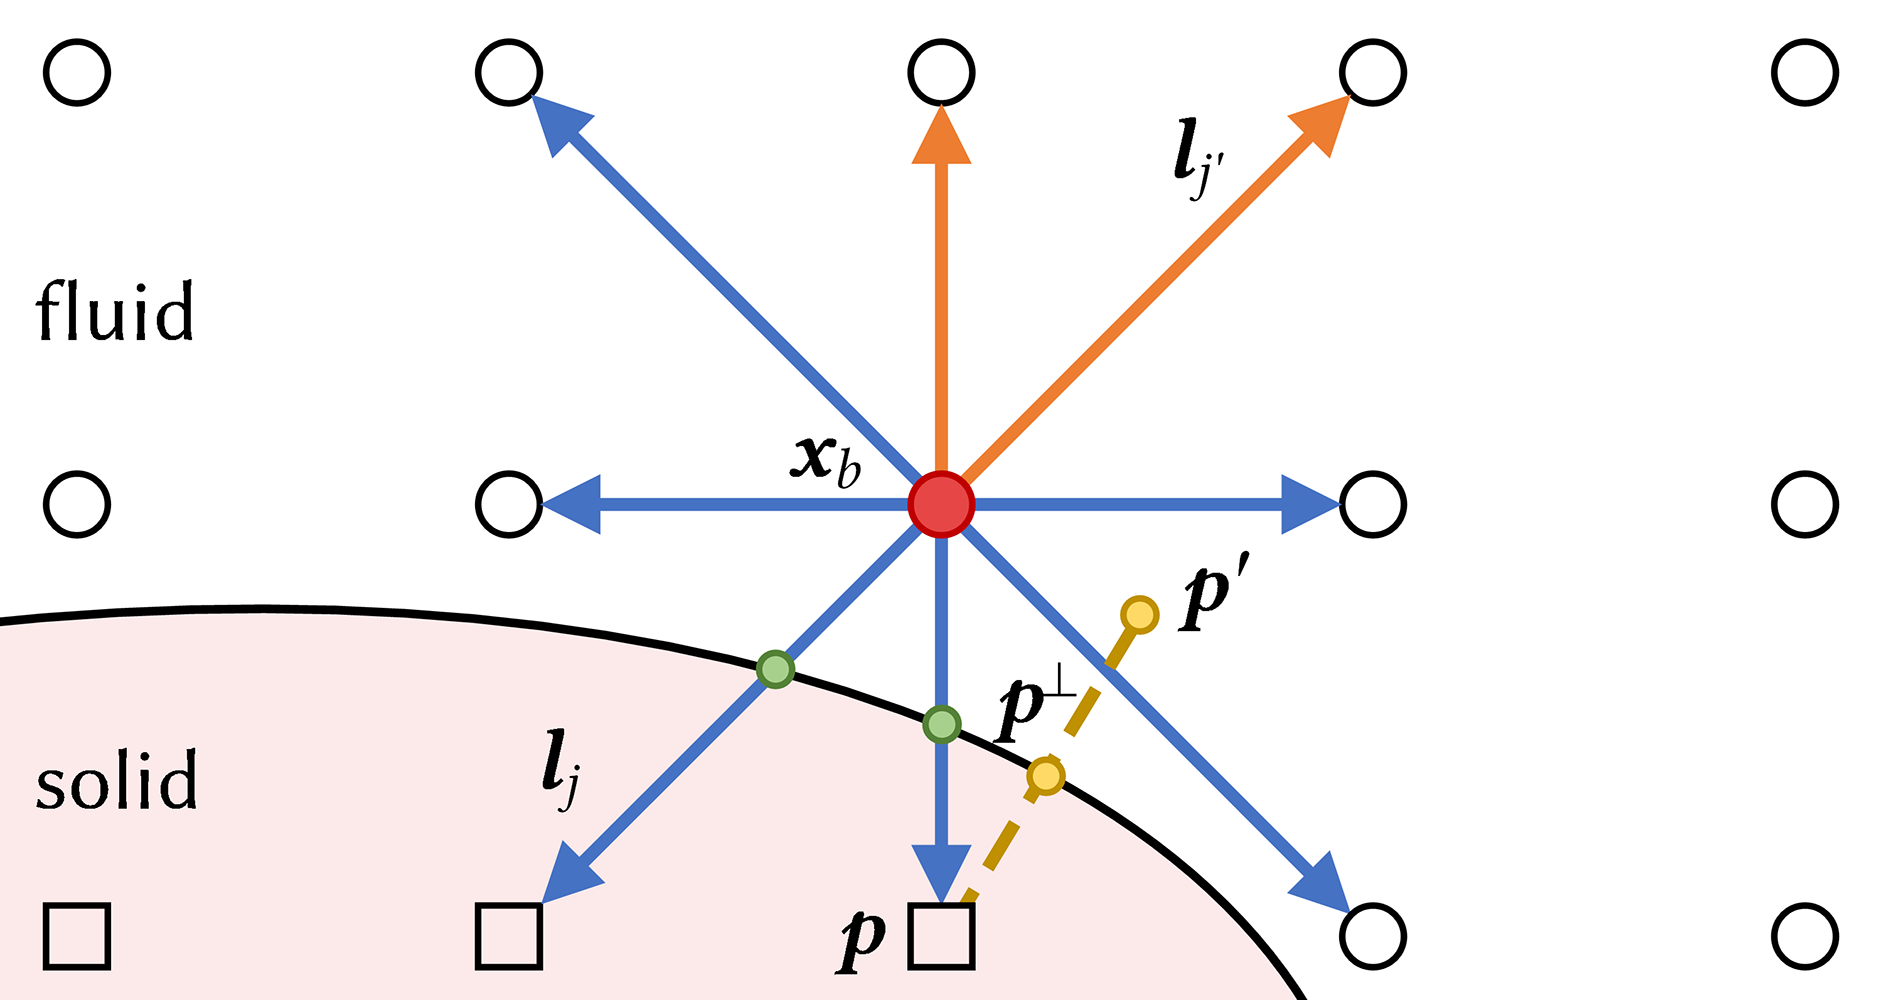
\includegraphics[width=0.75\columnwidth]{figures/bounce_back_scheme.png}
    \bicaption{固体边界的简单反弹方法与锐利界面浸入边界法。在迁移过程中,固体边界附近的流体格点$\bm{x}_b$ (图中标为红色圆圈) 的一部分分布函数$f_{j'}$ (图中标为橘色箭头) 是未知的,因为格点$\bm{x}_b-\bm{l}_{j'}$在固体内部 (图中标为方框),从而需要使用线段$\bm{x}_b$至$\bm{x}_b-\bm{l}_{j'}$与边界的交点 (图中标为绿色圆圈) 的速度$\bm{u}_s$来实现简单反弹边界处理,或$\bm{p}^\perp$与$\bm{p}'$点来实现锐利界面浸入边界处理。}{Simple bounce-back scheme and sharp-interface immersed boundary near fluid-solid boundary. During streaming, some of the distribution functions $f_{j'}$ (corresponding to the orange links) at the fluid node $\bm{x}_b$ (red circle) near a solid boundary are unknown, since the node at $\bm{x}_b-\bm{l}_{j'}$ is located inside the solid region (shown as boxes), requiring a bounce-back scheme using the velocity $\bm{u}_s$ of the boundary velocity at the intersection point (green circles) between the line segment from $\bm{x}_b$ to $\bm{x}_b-\bm{l}_{j'}$ and the solid boundary, or sharp-interface immersed boundary using $\bm{p}^\perp$ and $\bm{p}'$.}
    \label{img:bounce_back_scheme}
\end{figure}

\subsection{插值反弹边界}
简单反弹边界的一个问题是只有边界在速度方向中点时,边界处理的精度才可达到二阶。边界处于其他位置时,边界处理的精度只有一阶。
针对这一问题,插值反弹边界 (Interpolated bounce-back, IBB) 被提出~\cite{Bouzidi-2001},通过考虑边界到格点的距离,进行分布函数的插值:
\begin{equation}\label{eq:ibb_2001}
    f_i(\mathbf{x}_B, t+1) = 
    \begin{cases}
        2 q f^{*}_{\bar{\imath}}(\mathbf{x}_B, t)+(1-2 q) f^{*}_{\bar{\imath}}(\mathbf{x}_{F}, t), & q < 0.5, \\
        \frac{1}{2 q} f^{*}_{\bar{\imath}}(\mathbf{x}_B, t)+\frac{2 q-1}{2 q} f^{*}_i(\mathbf{x}_B, t), & q \geq 0.5,
    \end{cases}
\end{equation}
其中$q=\|\mathbf{x}_B - \mathbf{x}_W\|/\|\bm{c}_i\|$是边界点到边界的正则化距离。

在引入基于距离的插值后,反弹边界可以达到二阶精度,但是依然有一些问题。首先是公式~\ref{eq:ibb_2001} 引入了邻居点参与计算,对于GPU实现会降低数据访问效率。其次,当处理复杂外形的几何时,格点可能处于两个边界之间,导致找不到邻居点从而无法完成边界处理。最后,如第~\ref{sec:1_related_works_LBM} 节所介绍的,IBB在Bouzidi等~(\citeyear{Bouzidi-2001}) 后成为了一类方法,之后的工作提出了诸多不同的构造形式,甚至参数化的构造。这些不同的构造的性能与精度均有所区别。关于这一部分我们将在第\ref{sec:sig23}章中继续讨论。
\chapter{面向CG的通用边界处理方法}
\label{sec:siga21}

% Sec 3.1
\section{背景与动机}
流固耦合对于复杂的视觉现象仿真有很重要的作用,流体和固体之间的相互作用对两者的运动皆有影响,从而成为一个时间上的迭代过程。这种相互作用在数值上的计算是非常复杂的,并且,在有薄壳或细棒的场景中,流固耦合的计算是更加艰巨的。我们这里定义的薄壳或细棒是在某一个或某两个维度上非常狭窄的物体,以至于在这些维度上,物体的大小是远小于网格的尺度的。由于薄壳或细棒的这种特性,它们的特征在网格中很难被捕捉到,以至于经常发生泄漏或穿透等现象。

虽然有工作展示了薄壳~\cite{DiscreteShells,Bridson:2003} 或细棒~\cite{DiscreteRods} 的仿真,也包括它们在黏性流体~\cite{Fei-2018,Takahashi:2019,Fei-2019} 或非湍流~\cite{Azevedo-2016} 中的耦合,在动力学方法中使用扩散界面浸入边界法可以在湍流中或者更加稳定、高效的仿真结果~\cite{Li-2018,Li-2020}。

在本章中,我们介绍一个在LBM框架下的高效且通用的双向流固耦合边界处理方法,以可同时求解固体任意维度为亚网格尺度的情况。我们的方法将简单反弹边界方法与一个速度修正方法混合,以克服之前方法的缺点,提升仿真的稳定性与视觉效果。并且,通过几何上的近似,与实现层面的GPU优化,我们的方法相比Chen等~(\citeyear{Chen-2021}) 提出的LBM优化方案,在仿真效率上有着数倍的提升。

因为LBM使用笛卡尔网格来离散空间空间,而固体的边界一般不与网格对齐,于是出现了切削网格的概念,即网格被固体边界所切割,如图~\ref{img:cutcell_and_interpolation} 中的绿色网格。一般在LBM中需要对切削网格进行特殊处理,以刻画流体与固体间的相互作用。现有的各类基于切削网格的边界处理方法虽不能在效率、准确度、稳定性上都尽善尽美,但也有各自的优势。如扩散界面浸入边界法不需要追踪网格随物体的变化,从而降低了求解的复杂度。但它通过施加惩罚力来描述边界对流体的作用,不能准确刻画边界的形状,从而不适用于薄物体的仿真,如图~\ref{img:cutcell_and_interpolation} 所示。而简单反弹边界方法虽然可以通过分布函数的反弹阻止流体泄露 (即使是薄物体),但是因为它的准确性有限,在仿真中会产生不正确的速度分布,影响仿真的稳定性,如图~\ref{img:Immersed_Bounce_back}所示。

我们提出混合方法的一个重要动机是,这两类方法实质上是互补的。在反弹边界方法中,介观尺度的分布函数反弹从宏观上看,构成了部分浸没边界法中所需的惩罚力。而其本身又有着可以防止流体穿过薄物体的性质,所以我们可以施加一个额外的辅助惩罚力,对反弹边界法进行修正。我们注意到这个辅助惩罚力会比浸没边界法中原本的惩罚力要小很多。这样的混合方法可以满足我们在正确求解薄物体的同时,对精度与效率的需要。

\begin{figure}[htb]
    \centering
      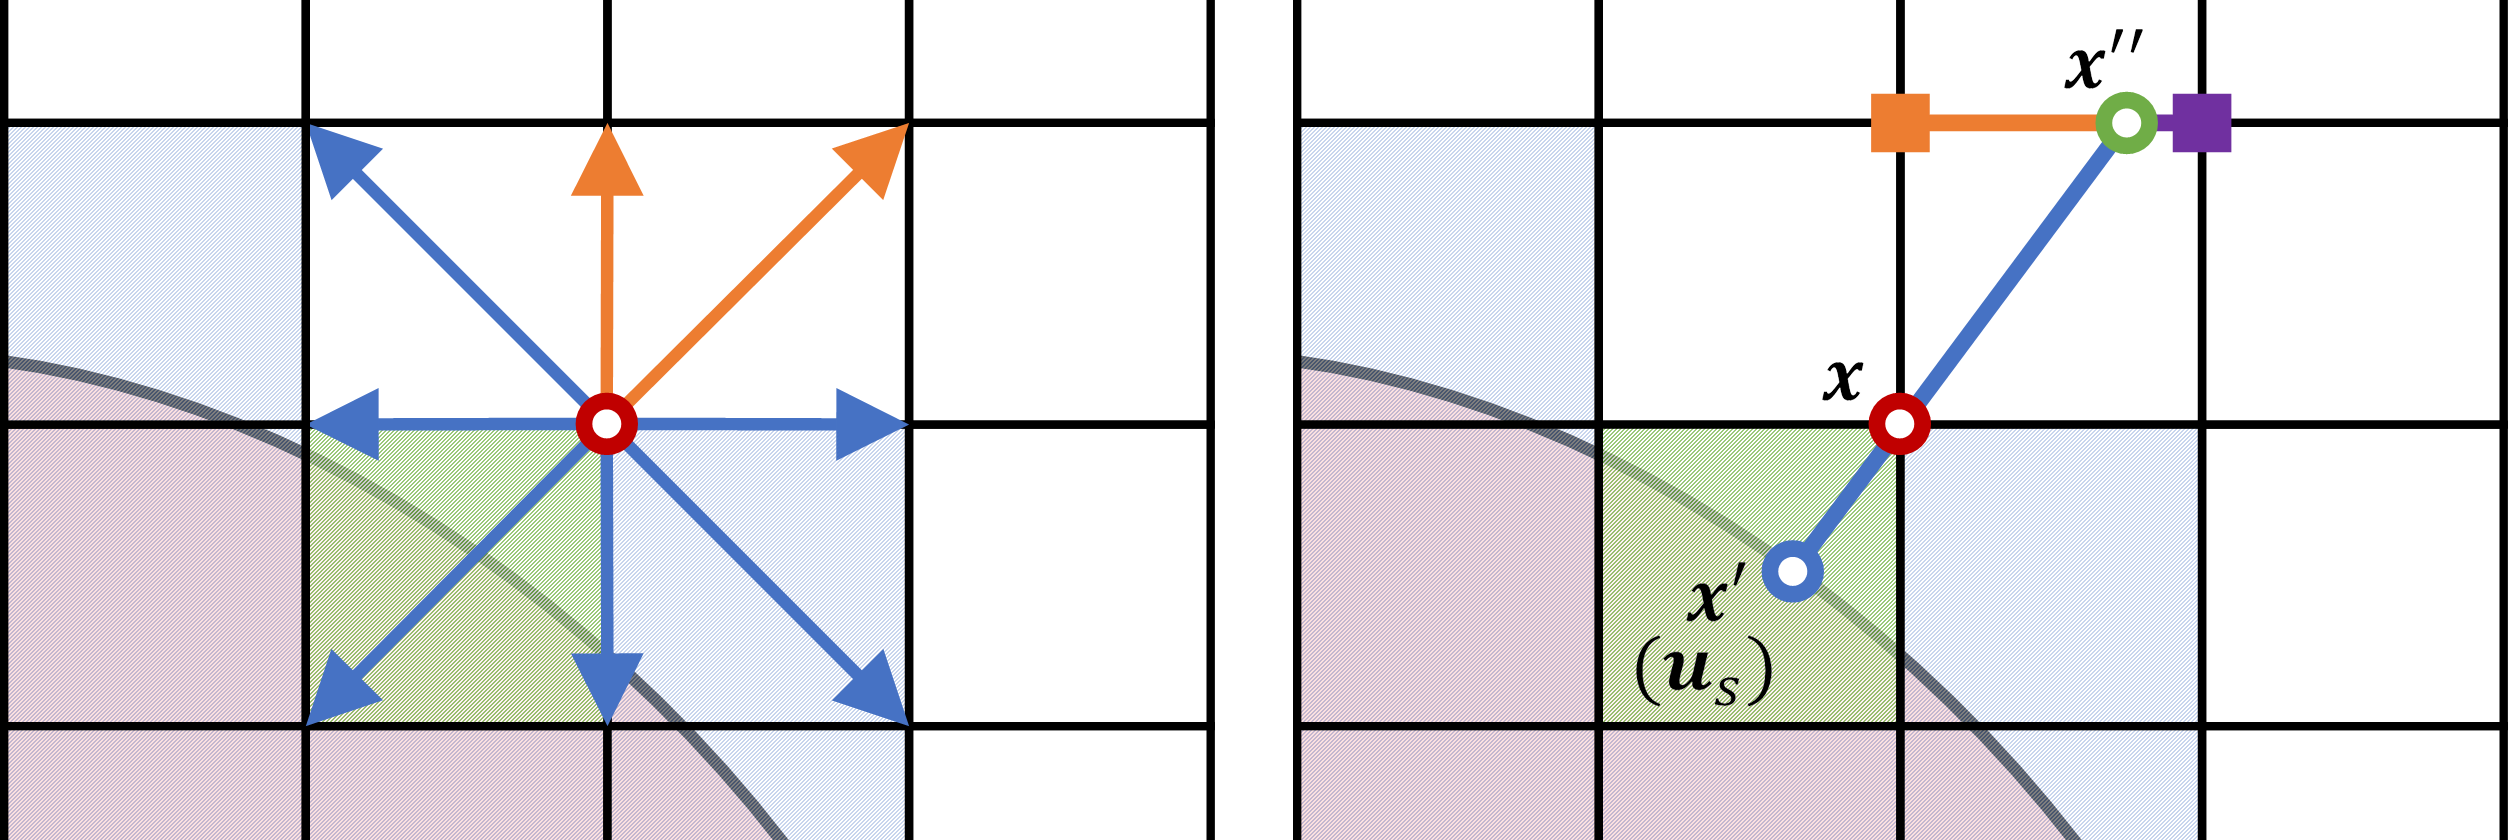
\includegraphics[width=0.95\columnwidth]{figures/cutcell_and_interpolation.png}
    \bicaption{切削网格中的速度插值。左图:因为固体边界存在而产生的切削网格 (图中标为绿色)。右图:流体中的切削网格格点$\bm{x}$ (图中标为红色圆圈) 的速度,需要通过固体边界的投影点$\bm{x}{'}$ (图中标为蓝色圆圈),与该投影点到格点的延长线与下一个网格的交点$\bm{x}{''}$ (图中标为绿色圆圈) 进行速度的线性插值得到。}{Interpolation of velocity on cut-cell nodes. Left: cut-cell (marked in green) intersecting a solid boundary; Right: the velocity on a cut-cell node $\bm{x}$ inside the fluid region (red circle) needs to be interpolated using the velocities of its projected point $\bm{x}{'}$ onto the solid boundary (blue circle) and the intersected point between the ray from the projected point to the cut-cell node and the interpolated fluid point $\bm{x}{''}$ (green circle), where the velocity can be reliably evaluated through simple linear interpolation.}
    \label{img:cutcell_and_interpolation}
\end{figure}

\begin{figure}[htb]
    \centering
      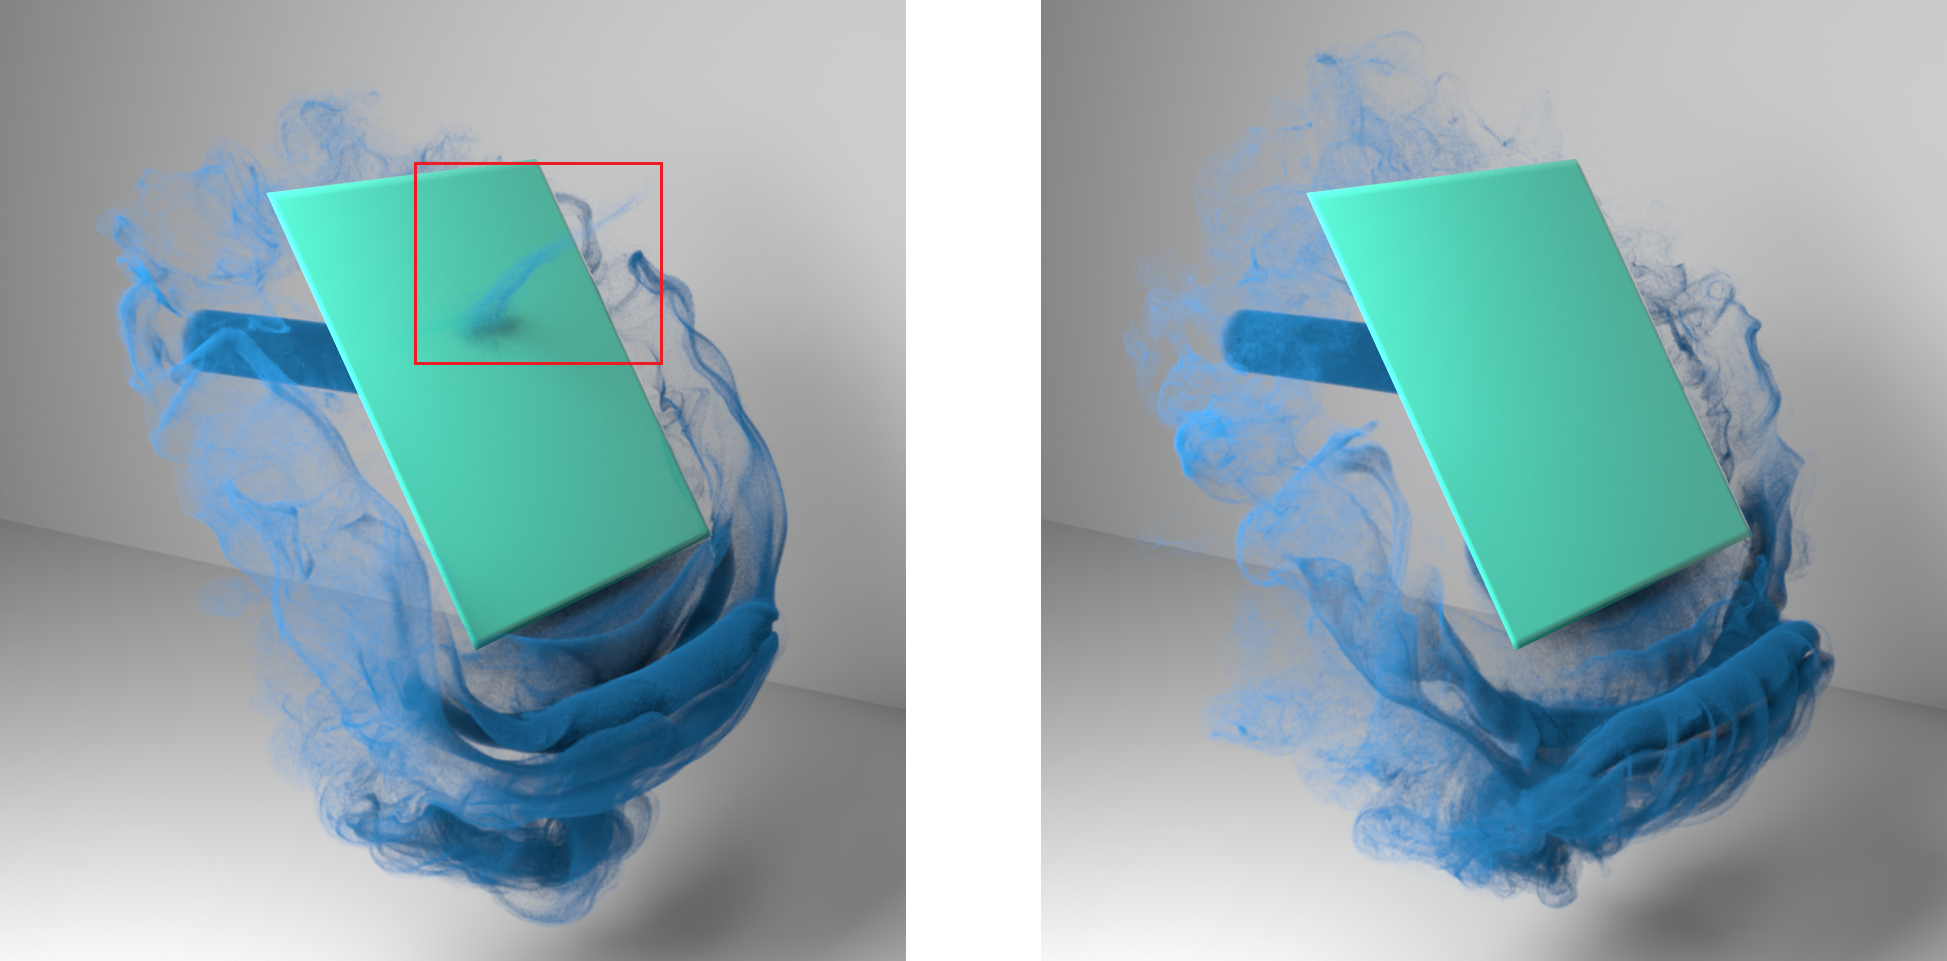
\includegraphics[width=0.97\columnwidth]{figures/comparison_with_ib.png}
    \bicaption{浸没边界法造成的泄露。当有薄板存在时,Li等~(\citeyear{Li-2020}) 所使用的浸没边界法 (左图) 与我们的方法的对比 (右图)。因为惩罚力会分布到薄板两侧,扩散边界浸没边界法可能会产生泄露 (见图中红色方框),而我们的方法可防止此现象。}{Leakage of immersed boundary. For a kinetic fluid simulation coupled with a thin plate, the immersed boundary method used by Li et al.~(\citeyear{Li-2020}) (left) is compared with our method (right). Due to force spreading in both sides of the thin plate, this recent coupling approach employing a diffuse-interface immersed boundary method may generate leakage through the plate (see red box), while our method prevents this issue by design.}
    \label{img:comparison_with_ib}
\end{figure}

\begin{figure}[htb]
    \centering
      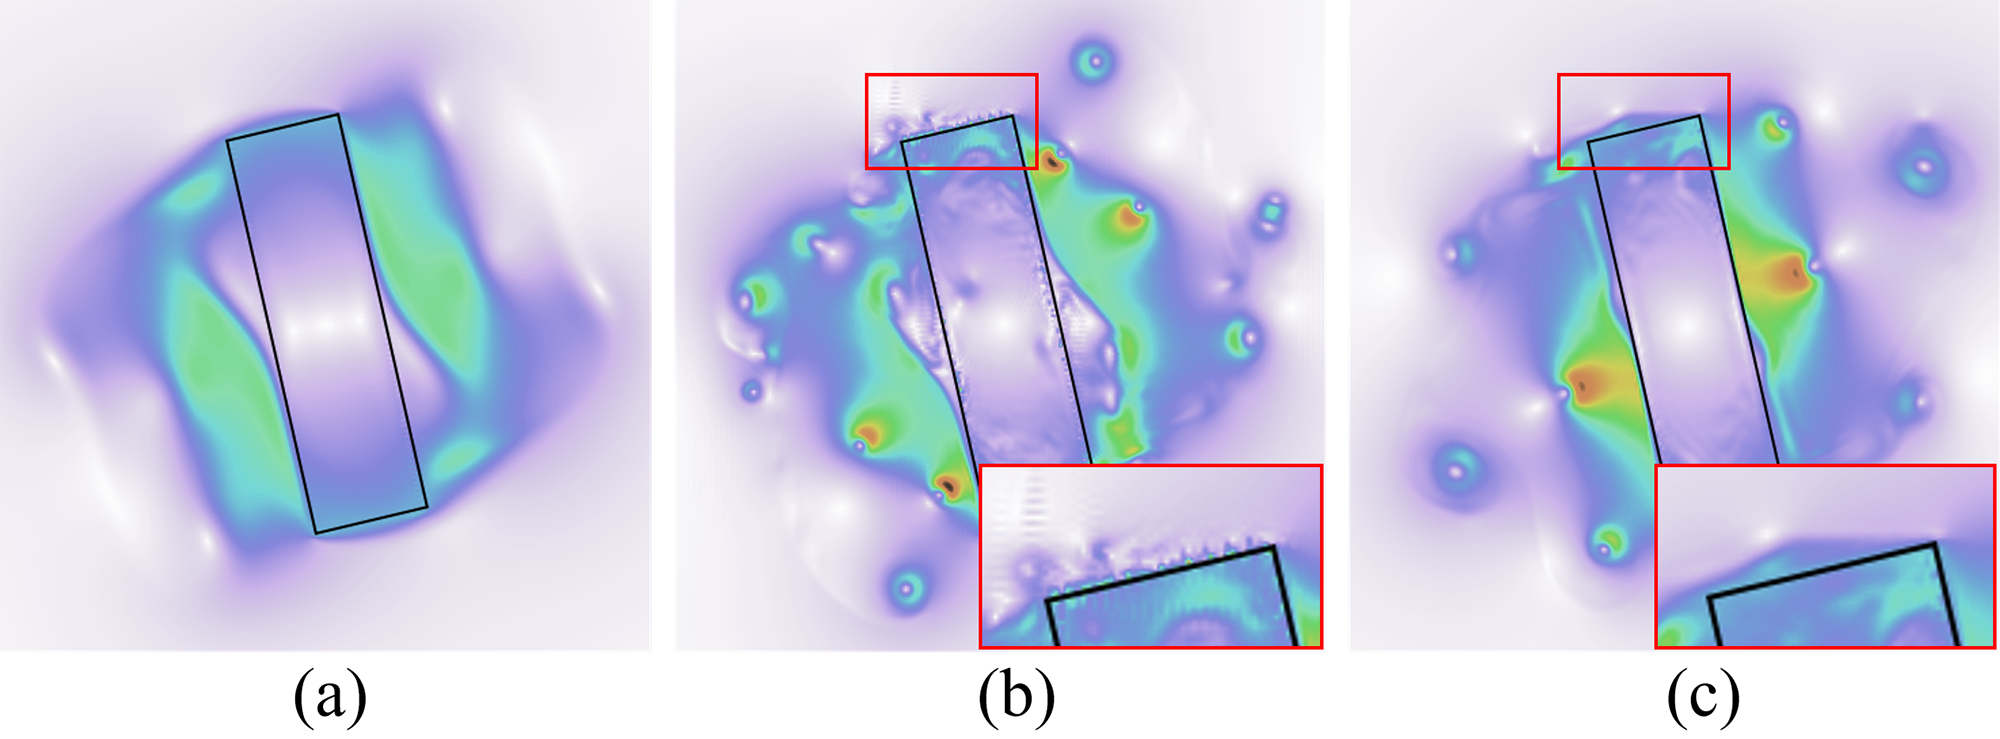
\includegraphics[width=0.95\columnwidth]{figures/ib-mbb.png}
    \bicaption{不同雷诺数下的简单反弹边界处理方法。(a) 在低雷诺数下,简单反弹边界没有造成视觉不正确的现象;(b) 但在高雷诺数下,固体边界会有很强的锯齿现象,从而对稳定性有较大影响;(c) 我们的方法在与 (b) 同样的高雷诺数情况下看不到视觉不正确的现象。}{Simple bounce-back under different Reynolds numbers. (a) a plain simple bounce-back scheme generates no visual artifacts for  flows with low Reynolds number; (b) however, it exhibits strong aliasing artifacts near the solid boundary for high Reynolds number flows, which may seriously influence stability; (c) our new boundary treatment for the same high Reynolds number as in (b) is artifact-free, generating the type of vortices expected from such an example.}
    \label{img:Immersed_Bounce_back}
\end{figure}

% Sec 3.2
\section{方法}
我们的混合方法主要包含下面三个部分:
\begin{itemize}
\item 双面简单反弹边界:我们首先介绍一个简单反弹边界方法的变种,即切削网格边界的两侧都会发生分布函数的反弹,而不只在一侧发生,从而不再需要追踪格子随物体运动的状态变化;
\item 切削网格的速度修正:我们通过在切削网格内进行单边的速度修正,大幅提升仿真的稳定性,同时压制边界上的速度误差;
\item 固体受力:最后我们通过介观与宏观的混合,求出流体转移至固体的动量,从而获得固体受力以驱动固体运动。
\end{itemize}

我们将在下面依次介绍这三部分内容。

\subsection{双面简单反弹边界}
在第~\ref{sec:boundary_treatment} 节中,我们回顾了简单反弹边界方法。一般来说,反弹边界都只应用于流体点。然而随着物体的运动,流体点可能被固体覆盖成为固体点,固体点也可能重新变为流体点。这个转换过程不止需要追踪格点状态,并且需要进行速度的插值,甚至外插。这样会在高雷诺数下在固体边界上产生很强的耗散误差。为了避免这一现象,我们对所有切削网格内的点都进行分布函数反弹,而不只针对流体点。我们称该方法为\emph{双面简单反弹边界方法}。该方法依旧可以避免流体泄露,即使有亚网格物体存在。但这并没有改善固体边界的速度锯齿现象与大速度梯度造成的误差,所以我们引入下一节中介绍的速度修正方法。

\subsection{切削网格的速度修正}
因为我们谋求的是低阶 (线性) 精度的边界处理,我们提出在双面简单反弹边界之后,通过沿固体边界的法向方向对速度线性插值,来对速度场进行修正。修正的方式为对流场施加惩罚力。更具体地说,我们先通过切削网格点周围的固体和流体速度插值,得到一个切削网格点上的期望速度。之后通过当前速度与期望速度的差计算惩罚力,从而修正速度场。

\paragraph{切削网格点上的期望速度}
切削网格点上的期望速度可通过其邻近的可靠速度插值得来。对于处于固体内部的切削网格点,它们的期望速度必须与那一点的固体速度一致,这个速度可以通过固体的运动状态直接获得。
对于流体中的切削网格点,我们通过一个线性插值,获得其期望速度。该插值方法如图~\ref{img:cutcell_and_interpolation} 中右图所示。对于切削网格点$\bm{x}$点,我们首先计算它在固体边界的投影点位置$\bm{x}'$,之后从$\bm{x}'$向$\bm{x}$打一条射线,该射线与下一个网格面的交点为$\bm{x}''$。如果这个面上的所有点都不是切削网格点,$\bm{x}''$点的速度就可以通过该面上的点线性插值得来 (二维中是线性插值,三维中是双线性插值)。如果这个面上存在点是切削网格点,则可寻找下一个交点,直到找到满足条件的交点。此时$\bm{x}$点的期望速度则可通过线性插值得到:
\begin{equation}  \label{eq:vel_lerp}
\hat{\bm{u}}(\bm{x})=(1-\alpha)\bm{u}_s + \alpha \bm{u}(\bm{x}'')\;,
\end{equation}
其中$\alpha=\|\bm{x}-\bm{x}'\|/\|\bm{x}''-\bm{x}'\|$,$\bm{u}_s$是固体边界上投影点$\bm{x}'$的速度。

\paragraph{基于惩罚力的速度修正}
由于切削网格点$\bm{x}$上的期望速度$\hat{\bm{u}}(\bm{x})$可能与分布函数反弹后的宏观速度$\bm{u}(\bm{x})$有偏差,我们构造如下的惩罚力$\bm{F}_p(\bm{x})$
\begin{equation} \label{eq:penaltyForce}
\bm{F}_p(\bm{x}) = \hat{\bm{u}}(\bm{x})-\bm{u}(\bm{x})\;,
\end{equation}
施加在点$\bm{x}$上,做法与Li等~(\citeyear{Li-2020}) 中相同。我们将惩罚力投影至分布函数空间,分布函数使用最高阶的埃尔米特多项式展开,以维持精度与稳定性。由于反弹边界已经承担了大部分的边界处理,这里的惩罚力会比传统浸没边界法中的惩罚力小很多,只作为一个速度的修正出现,于是我们也不需要采用Li等~(\citeyear{Li-2020}) 中的时间重缩放来缩短物理时间步长从而提升稳定性。这可以使仿真效率进一步提升。

\begin{figure}[htb]
    \centering
      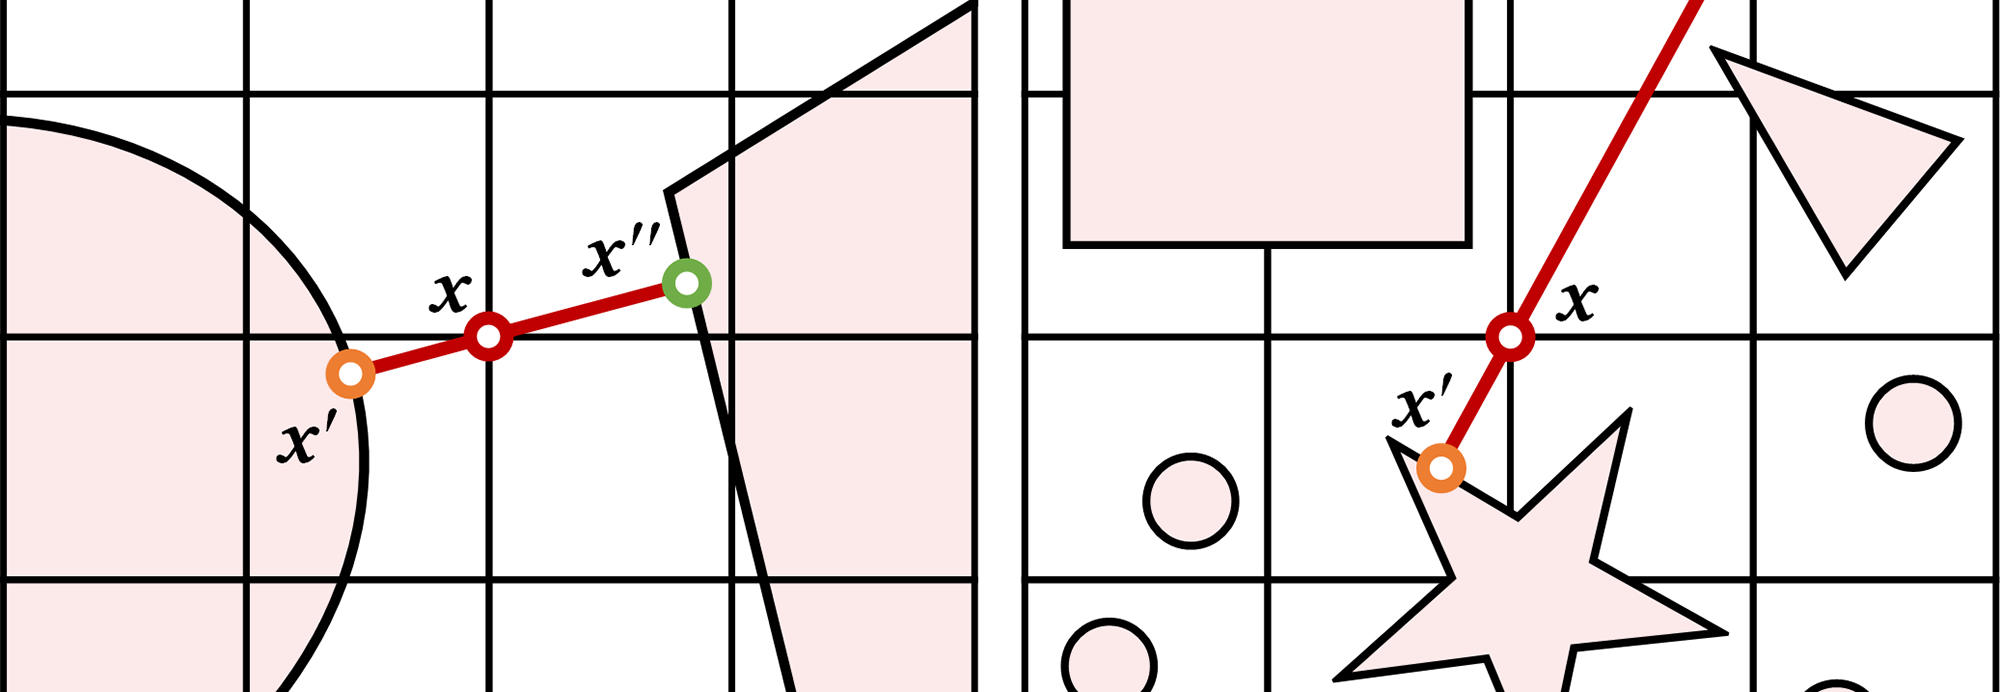
\includegraphics[width=0.95\columnwidth]{figures/cutcell_special_cases.png}
    \bicaption{两种邻近物体的情况。左图:从固体边界点$\bm{x}'$起始的射线经过$\bm{x}$点,在交到网格面之前,便相交于另一个物体上。这种情况,$\bm{x}''$是另一个固体边界点。右图:一个切削网格点可能完全被切削网格面包围,所以找不到任何非切削网格面。}{Two cases of solid proximity. Left: the ray starting from a boundary point $\bm{x}'$ through a grid node $\bm{x}$ may hit another boundary surface point before it intersects with the non-cut-cell face; in this case, $\bm{x}''$ locates at another boundary point. Right: a cut-cell node may be surrounded by all cut-cell faces, so a ray may not hit any non-cut-cell face nearby.}
    \label{img:handling_proximity}
\end{figure}

\paragraph{一些特殊情况}
当流体中的物体间距离接近网格尺度的时候,有时$\bm{x}''$的速度会无法从周围的非切削网格点插值得到。一种情况是从$\bm{x}'$点射出的射线在交到网格面之前,便相交于另一个物体上 (图~\ref{img:handling_proximity} 中左图)。那么由于这个交点的速度是已知的,我们可以用这一速度替代先前提到的非切削网格点的速度。另一种情况是,因为物体之间过于接近,射线无法找到任何非切削网格面。这个时候我们只得抛弃速度修正过程,而只采用双面简单反弹边界作为边界处理。

\begin{figure}[htb]
  \centering
    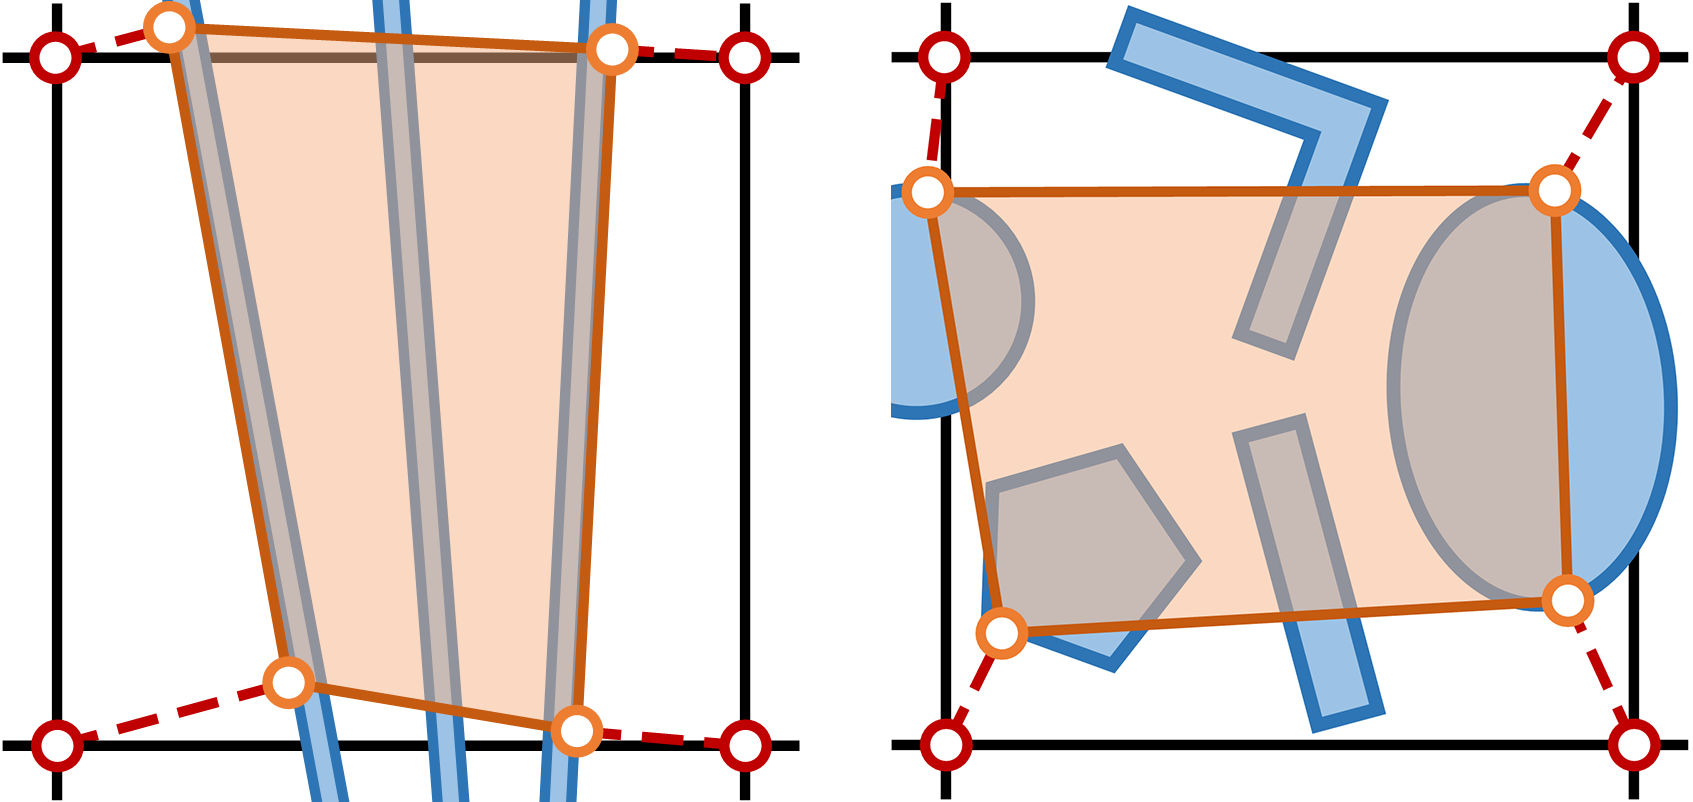
\includegraphics[width=0.9\columnwidth]{figures/sub_grid_approximation.png}
  \bicaption{亚网格近似。在亚网格物体存在时,我们将每个切削网格点投影至其最近的边界采样点。这等同于使用一个包围体积 (橘色区域) 来近似一个网格中的多个亚网格物体。}{Sub-grid approximation. To handle sub-grid scale solid structures, we project each cut-cell node onto its nearest boundary sample point. This basically amounts to using bounding volumes (orange regions) to approximate multiple thin structures within a cut-cell.}
  \label{img:sub_grid_approximation}
\end{figure}

\paragraph{亚网格近似}
当数量众多的薄板或细棒存在时,有可能一个流体网格中会包含多个这样的物体,尤其在网格较粗的情况中 (见图~\ref{img:sub_grid_approximation} ),此时边界的精度是无法保证的。此时,我们使用一个包围体积,来近似这些存在于一个网格中的多个物体。所以我们依然可以将流体点投影至距离最近的固体边界点来计算惩罚力。

\paragraph{讨论}
我们的惩罚力修正是基于法向方向的线性速度插值。这个修正可被认为是一个滤波器,来压制在高雷诺数下,简单反弹边界造成的固体边界周围的速度震荡。这个修正可以有效地提升在湍流流固耦合仿真的稳定性,使得我们在相对粗糙的网格中也能获得视觉上可信的仿真结果。然而,这依然只是一个一阶的线性修正,所以要获得高物理精度的仿真需要高分辨率网格作为基础。但考虑到我们主要面向图形学应用,我们不考虑在构造更加复杂的速度修正方法。

\subsection{固体受力}
因为要做到流固的双向耦合,我们需要讨论流体中固体的受力,也即流体传递给固体的动量。我们在边界中使用了反弹边界与速度修正的结合,所以我们在讨论固体受力时也分为两部分来讨论。我们首先讨论双面反弹边界对固体受力的贡献。在双面反弹边界之后,我们先将由公式~\ref{eq:bounce-back} 带来的动量交换进行累计。更具体地说,迁移过程后,$t$时刻$\bm{x}$点的动量可以表达为
\begin{equation}
  \bm{p}(\bm{x}) = \sum_{i}\bm{c}_if^*_i(\bm{x},t).
\end{equation}
如果$L$是$\bm{x}$点切削速度方向的集合 (即与固体边界相交的速度方向),每一个$L$中的速度方向都会发生分布函数反弹,那么$\bm{c}_j$方向的流固动量交换是
\begin{equation}
  \smash{-\bm{c}_{j}\,(f^*_{j}(\bm{x}) + f^*_{j'}(\bm{x}))}.
\end{equation}
从而,在$\bm{x}$点交换的动量和$\Delta \bm{p}$为
\begin{equation}
\Delta \bm{p}(\bm{x})= - \sum_{j\in L} \bm{c}_{j}\,(f^*_{j}(\bm{x}) + f^*_{j'}(\bm{x})),
\end{equation}
其中我们不将$(\Delta x)^3$显式写出 ($\Delta x$是网格大小),因为在正则化LBE空间中这一项为1。
那么反弹边界部分所贡献的固体受力是所有点动量交换的和,即
\begin{equation}
\bm{F}_{B}\equiv \sum_{\bm{x}} \Delta \bm{p}(\bm{x}),
\end{equation}
其中除以$\Delta t$ (时间步长) 也被隐去,因为其在正则化LBE空间中也为1。类似地,我们可以获得总的力矩
\begin{equation}
\bm{\tau}_{B}\equiv \sum_{\bm{x}} (\bm{x}-\bm{x}_{C})\times\Delta \bm{p}(\bm{x}),
\end{equation}
其中$\bm{x}_{C}$是物体质心的位置。

接下来我们继续讨论速度修正对固体受力的贡献。我们认为这个速度修正的来源依旧是固体的存在,所以这个力的来源是固体本身。那么固体理应受到一个与惩罚力大小相同,方向相反的反作用力。那么这一部分固体所受到的合力$\bm{F}_{C}$与合力矩$\bm{\tau}_{C}$可以表达为
\begin{equation}
\bm{F}_{C} = - \sum_{\bm{x}}\bm{F}_p(\bm{x}), \quad \bm{\tau}_{C} = - \sum_{\bm{x}} (\bm{x}-\bm{x}_{C})\times\bm{F}_p(\bm{x}).
\end{equation}

所以固体受到的合力$\bm{F}_s$与合力矩$\bm{\tau}_s$是上述两部分贡献的和:
\begin{equation}
\bm{F}_s = \bm{F}_{B} + \bm{F}_{C} \text{ and } \bm{\tau}_s = \bm{\tau}_{B} + \bm{\tau}_{C}.
\end{equation}

\section{算法优化}
\subsection{几何近似}
我们的混合边界处理中需要许多的几何计算,如将流体点投影至固体表面,或将速度方向与固体边界进行求交等。我们还需要识别切削网格点,以及它们的状态 (属于流体区域或固体区域)。许多工作阐述了如何准确地进行这样的几何计算~\cite{Azevedo-2016,Robinson:2009}。但由于固体边界的形状可能十分复杂,这一过程可能非常耗时,不利于维持LBM高并行度的优势。
为了在效率与精度间取得平衡,我们提出一系列的几何近似计算方法,以在不影响视觉可信度的情况下提升计算效率。

\begin{figure}[!htbp]
  \centering
    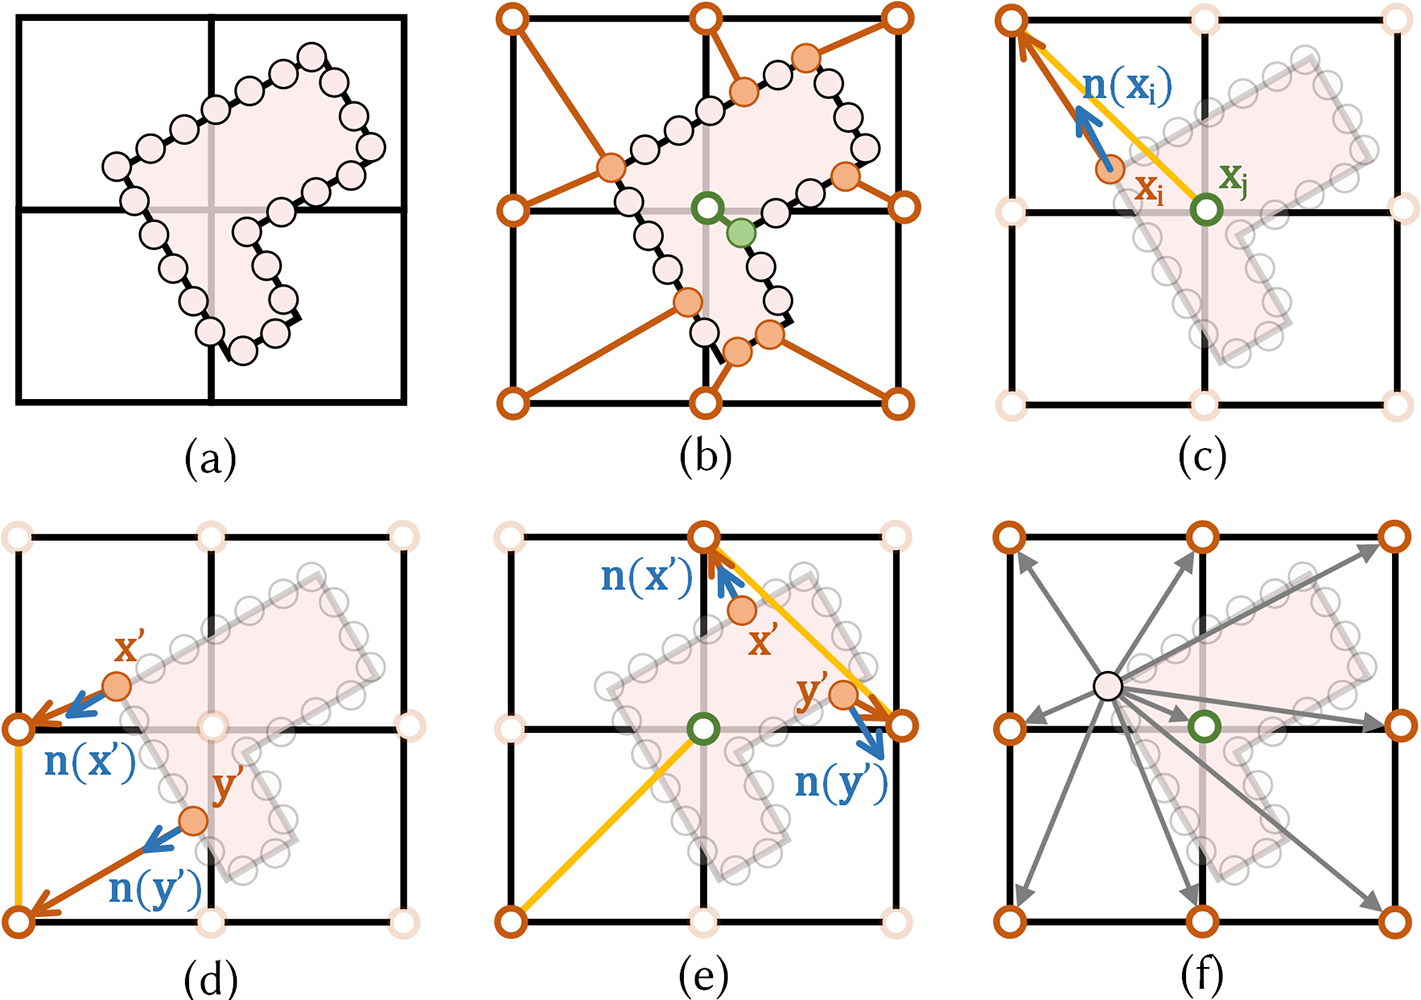
\includegraphics[width=0.97\columnwidth]{figures/geometric_computing.png}
  \bicaption{高效几何近似计算。对于一个固体,我们首先对它的边界采样 (a),然后切削网格点的投影点可以被近似为距其最近的采样点 (b)。为了检验某个速度方向 (图中标为黄色) 是否与固体边界相交,我们可以检查这个方向的两端是否有固体点存在。如果一端是固体点另一端是流体点,则我们认为其跨过了固体边界 (c) (图中绿色点为固体点,橘色点为流体点)。对于两端都是流体点的情况,我们检查这两个流体点投影点的法向,如果它们有类似的朝向 (d) 则认为该方向没有跨过边界,相反则认为其跨过边界 (e)。在GPU实现时,我们从所有的固体采样点出发,令每个固体采样点寻找其周围的流体切削网格点,而不是从流体点出发。}{Efficient geometric approximation. Given a solid geometry, we first sample its boundary (a); then the projected points of cut-cell nodes can be simply approximated by the nearest sample (b). To examine whether a link (yellow) crosses the solid boundary, we first check if solid nodes are involved. If the ends of the link are fluid and solid nodes, then it crosses the solid boundary (c) (green cut-cell nodes are inside the solid, whereas orange ones are in the fluid). For links connecting fluid nodes, we check the normals of the two projected cut-cell nodes forming the link; if the two normals have the same orientation (d), the link does not cross the solid boundary; otherwise, it intersects the solid boundary (e). For GPU implementation, we parallelize over solid samples instead of cut-cell nodes, where each solid sample will check its surrounding region of cut-cell nodes.}
  \label{img:geometric-computing}
\end{figure}

\paragraph{表面采样与切削网格识别}
为了加速计算,我们可以使用采样点而不是实际的几何来表达边界。这一过程需要对固体表面进行均匀采样,如使用泊松圆盘采样 (Poisson-disk Sampling)~\cite{dunbar2006spatial}。注意这也要求固体模型应该是密封的。每一个采样点$\bm{x}_s$在采样时可获得一个由边界朝外的法向$\bm{n}(\bm{x}_s)$。之后如果有网格中包含至少一个边界采样点,这个网格就可以被识别为切削网格 (如图~\ref{img:geometric-computing} (a))。

\paragraph{高效切削网格投影}
在几何计算中一个最重要的 (也可能是最耗时的) 部分是将流体点$\bm{x}$投影至固体表面上,以得到投影点位置$\bm{x}'$。传统方法可能会构建一个树形结构,然后搜索距离$\bm{x}$点最近的三角形~\cite{wang-2012}。在这里我们使用一个高效的近似算法来替代这一过程,我们在固体表面选择一个距离$\bm{x}$点最近的采样点$\bm{x}_s$,并满足
\begin{equation}\label{eq:is_in_fluid}
(\bm{x}-\bm{x}_s)\cdot \bm{n}(\bm{x}_s) \geq 0\;
\end{equation}
来近似采样点$\bm{x}'$。公式~\ref{eq:is_in_fluid} 这个约束可以避免我们选择到错误朝向的采样点。如果没有满足这个约束的采样点,那么这个点应该被标记为固体点 (如图~\ref{img:geometric-computing} (b))。这个基于采样点的技术可以达到很高的并行度,但精度很显然依赖于采样密度。所以在实现中,我们需要保证每个切削网格内有足够的采样点数。一般我们设置泊松圆盘采样的采样距离不超过网格大小的一半。

\paragraph{近似反弹边界处理}
在双面反弹边界处理中,我们必须要识别出与固体边界相交的速度方向 (见图~\ref{img:bounce_back_scheme} )。对于厚物体,由于我们已经对切削网格点属于流体点或固体点有所标记,我们只许对速度方向的两端点的状态进行识别。如果两个端点分别为流体点和固体点,则这个速度方向与固体边界有相交。但是对于薄物体,可能存在两端均是流体点,但依然与固体表面相交的情况。所以我们要进行特殊识别。
对于从$\bm{x}$至$\bm{y}$点的速度方向,我们检查这两个点的投影点$\bm{x}'$与$\bm{y}'$的法向朝向是否不一致,即$\bm{n}(\bm{x}')\!\cdot\!\bm{n}(\bm{y'})\!<\!0$ (如图~\ref{img:geometric-computing} (d)与(e))。
如果朝向不一致 (图~\ref{img:geometric-computing} (e) 即为此情况),则我们认为$\bm{x}$点与$\bm{y}$点处于边界的不同侧,所以这个速度方向是与固体表面相交的。则我们应在这个方向上进行反弹边界处理。

\subsection{GPU实现}
目前为止所描述的我们的算法,包括几何近似,我们都希望它们尽可能的简单,且只涉及局部计算。这样可以令GPU的实现较为简单直接,且有尽可能高的计算效率。在实现时我们应用了Chen等~(\citeyear{Chen-2021}) 中提出的加速技术,与一些针对我们算法设计的加速实现。这些实现方法在本节进行讨论。

\paragraph{存储布局}
对于LBM来说,在并行时一般是按方向的。即先计算$f_0$,之后计算$f_1$、$f_2$、……,以此类推。在这种情况下数组结构体 (Structure-of-arrays, SoA) 是更好的存储布局,因为SoA结构可以提升缓存利用率,从而提升整体性能~\cite{Chen-2021}。我们在实现中也同样使用SoA布局。

\paragraph{快速碰撞计算}
Chen等~(\citeyear{Chen-2021}) 还讨论了在碰撞过程中所需要的中心矩投影矩阵$\bm{M}(\bm{u})$的逆矩阵$\bm{M}(\bm{u})^{-1}$计算问题。作者们在其中提到逆矩阵应该使用解析式进行计算来保证碰撞的精度。然而由于解析式非常复杂,在GPU计算时,会占用过多的寄存器,导致GPU占用率低。但是我们注意到,如果将$\bm{M}(\bm{u})^{-1}$的解析式进行LU分解~\cite{fei2018three},分解后的三角矩阵中很多元素是非常接近于0的。所以我们可以将这些非常接近于0的元素置0,之后使用稀疏矩阵的数据格式进行存储。这样并不会影响整体计算的精度 (所造成的误差低于机器误差),但是寄存器使用量可以大幅减少。在同样的GPU上进行测试,我们的碰撞过程的效率约是Chen等~(\citeyear{Chen-2021}) 中碰撞过程的三倍。

\paragraph{并行的切削网格点识别与投影}
我们在上一小节讨论了我们算法中的一个关键步骤是将切削网格点投影到物体表面,这一过程可以通过寻找距离该点最近的固体采样点来近似。一般这一过程会将流体边界点作为并行单元,来搜索距其最近的采样点。但是这样会造成GPU负载不均衡,从而降低GPU占用率。
所以我们在这一过程中,将固体采样点作为并行单元。对于每一个采样点,我们计算该点到周围的切削网格点的距离 (见图~\ref{img:geometric-computing} (f)),并且比较这个距离与切削网格点当前记录的最近点的距离。如果距离更小的话则更新该采样点为最近点。因为多个线程可能会同时访问同一个流体点,这一过程需要使用原子比较计算。注意公式~\ref{eq:is_in_fluid} 依然需要满足,所以切削网格点状态可以被同时识别。
这样的好处是,每个固体采样点附近一定存在切削网格点,并且数量接近。这样可以大幅提升GPU的负载均衡,减少无用的线程造成的线程开销,提升GPU占用率。

\begin{figure}[!htbp]
  \centering
    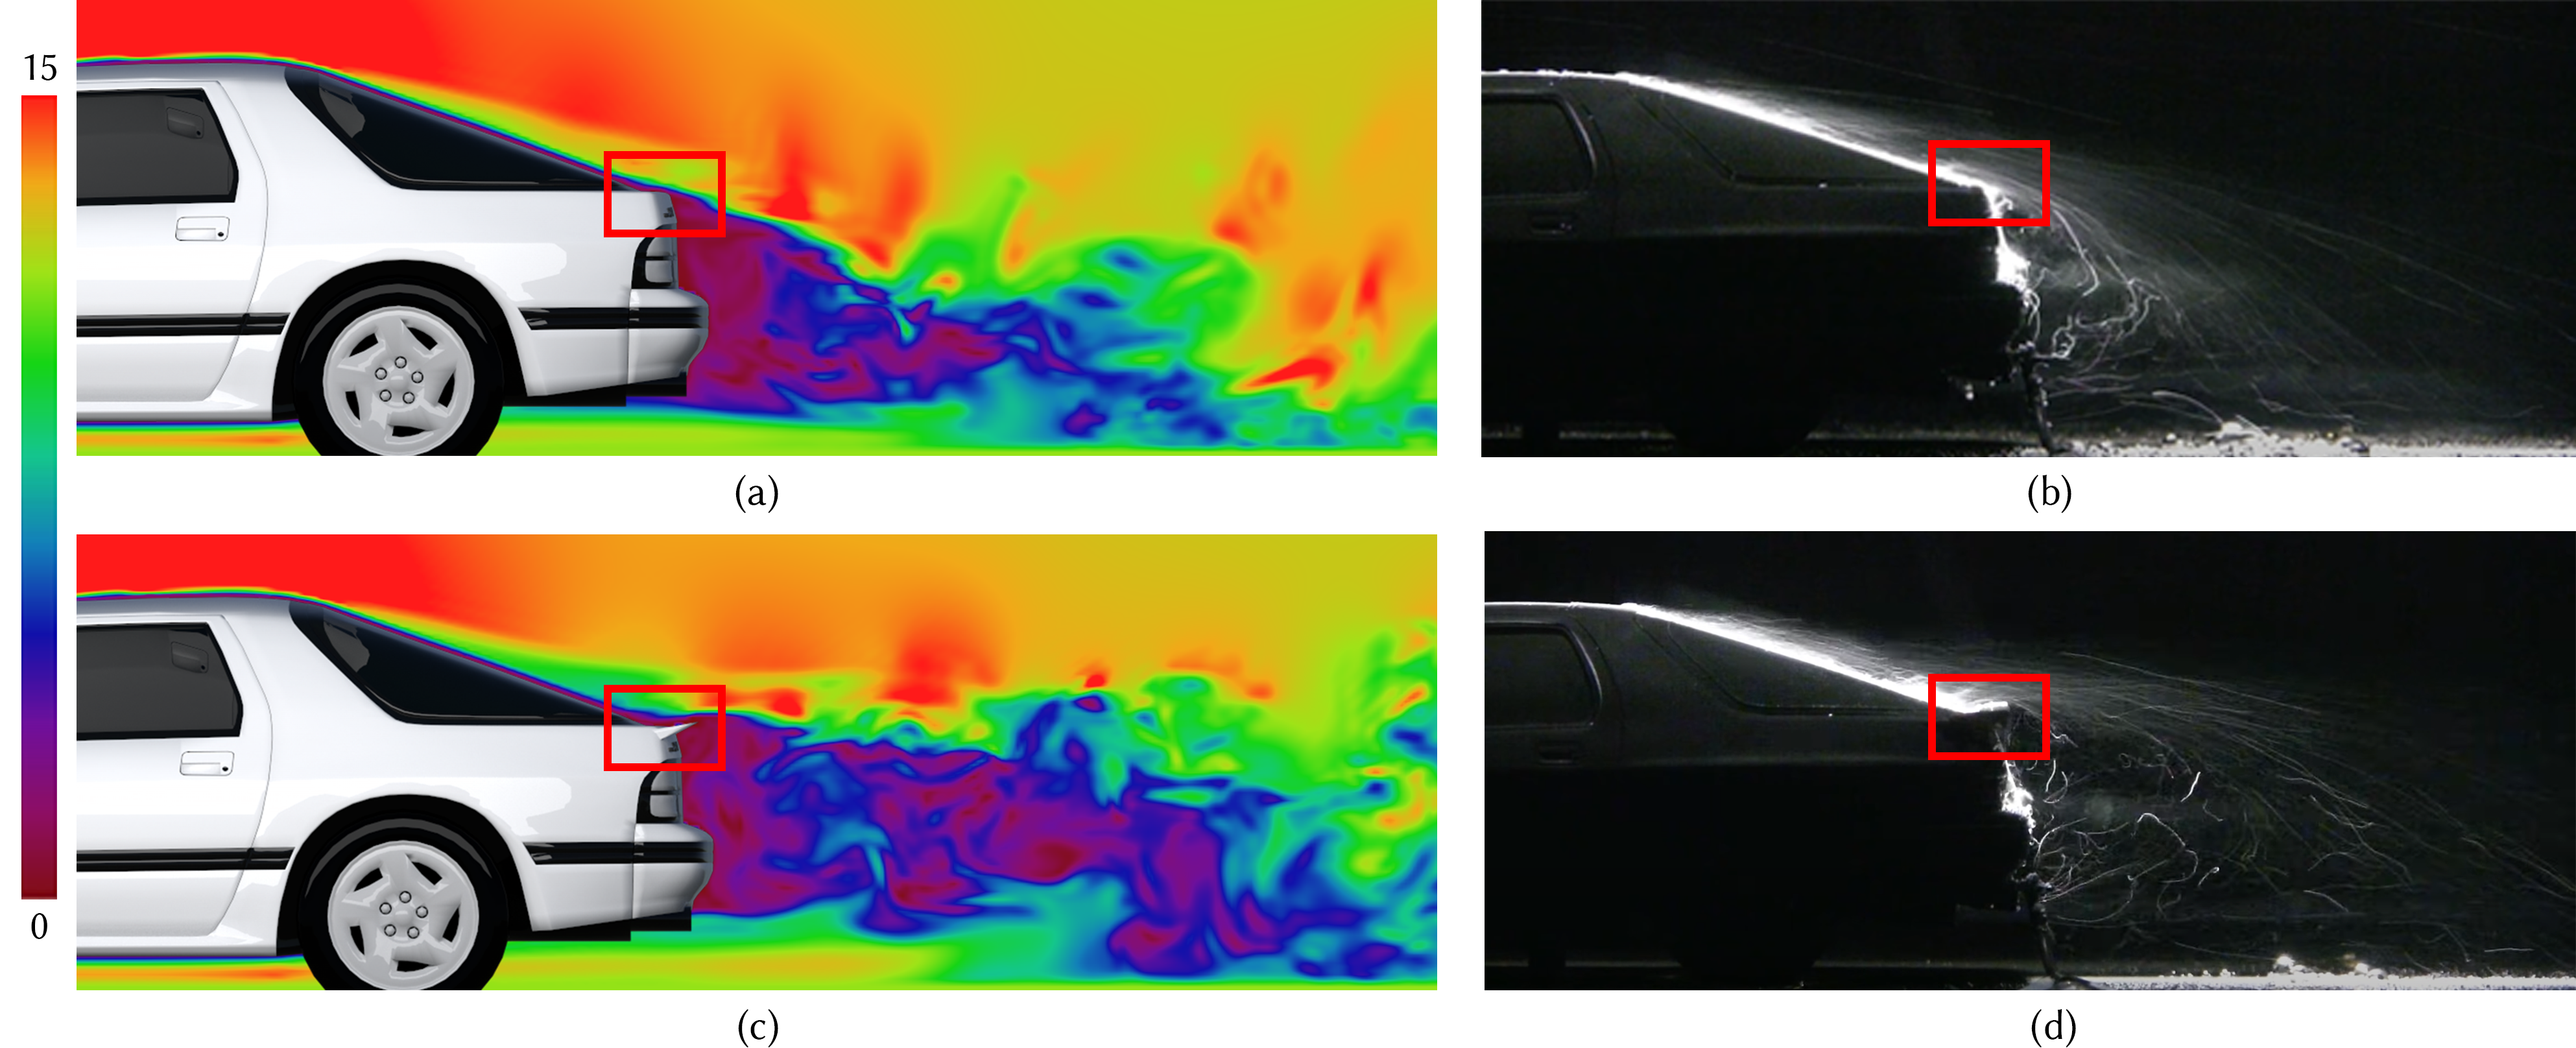
\includegraphics[width=0.99\columnwidth]{figures/comparsion_car_design.png}
  \bicaption{汽车的空气动力学设计。通过我们的方法对没有尾翼的汽车进行仿真 (a),其结果与一个相似的车辆模型在风洞可视化的结果匹配 (b)。之后添加一个小型的扰流板 (图中红色方框) 到汽车尾部之后,仿真中的尾流发生显著变化 (c),与带有扰流板的风洞测试相似 (d)。这展示出我们的方法可以快速、有效地为气动外形设计服务。图中的速度模值单位为$km/h$。图 (b) 与 (d) 的版权来自 Feltham~(\citeyear{youtube_2014})。}{Aerodynamic design of a car model. Simulating the airflow around a car model without a spoiler using our solver (a) matches the wind tunnel visualization for a similar car model (b); A small and thin spoiler (in red box) added on the back of the car model (c) changes the wake flow of the car model in our simulation quite significantly, in line with a wind-tunnel test of a car model with a spoiler (d) --- indicating that our solver offers an efficient, yet predictive tool of air flows for computational shape design. The velocity magnitude is measured in $km/h$. Image (b) and (d) courtesy of Feltham~(\citeyear{youtube_2014}).}
  \label{img:comparsion_car_design}
\end{figure}

\begin{figure}[!htbp]
  \centering
    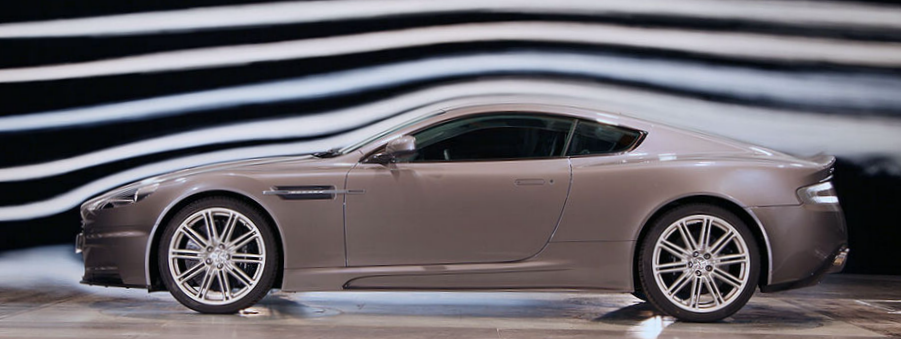
\includegraphics[width=0.99\columnwidth]{figures/car_wind_tunnel.png}
  \bicaption{车的风洞测试。车周围的气流可视化展示了车身的设计使得气流直到后备箱才发生边界层分离,这样可以有效减少风阻与震动。图片版权来自\textit{Auto Motor und Sport}, \copyright Frank Herzog/Sportauto.}{Wind-tunnel test of a car. A wind tunnel visualization of the airflow around a car shows that the design of the body delays boundary layer separation until the trunk, which reduces drag and vibration in practice. Image courtesy of \textit{Auto Motor und Sport}, \copyright Frank Herzog/Sportauto.}
  \label{img:car_wind_tunnel}
\end{figure}

\begin{figure}[!htbp]
  \centering
    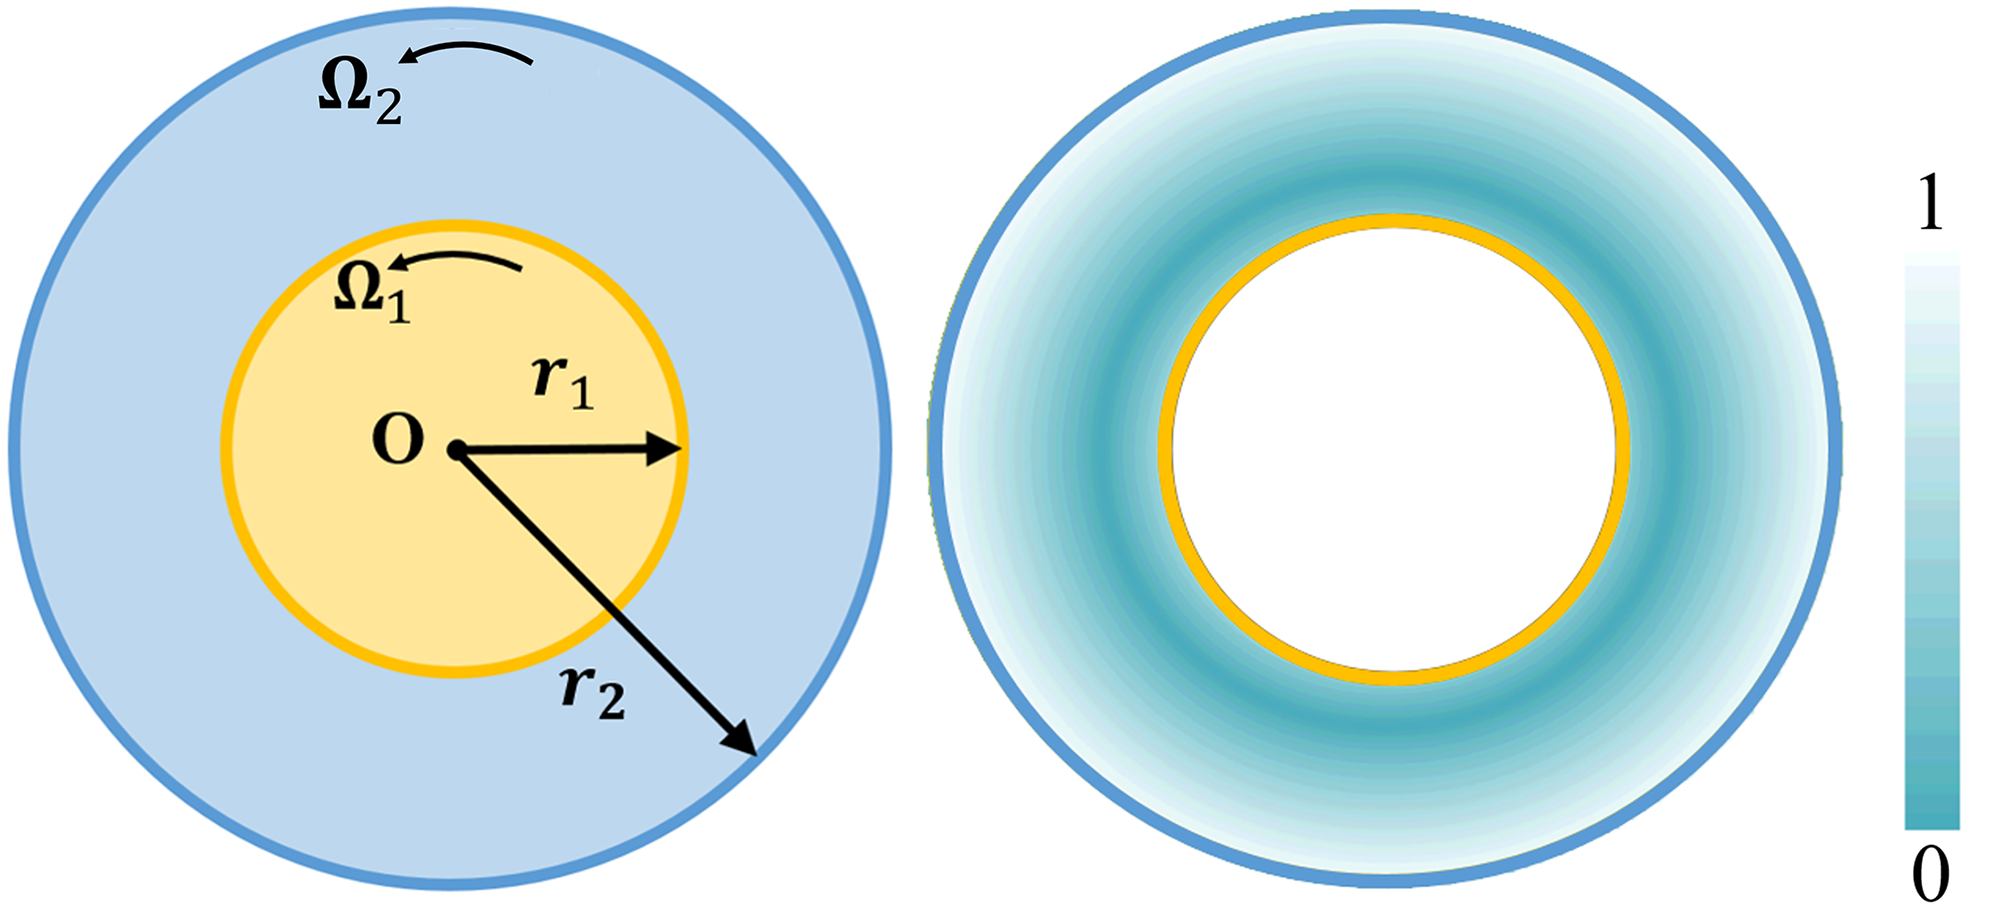
\includegraphics[width=0.85\columnwidth]{figures/taylor-couette-setting-2d.png}
  \bicaption{二维泰勒-库埃特流。左图:两个以$\bm{O}$点为圆心的同心圆,半径分别为$r_1$、$r_2$,角速度为$\Omega_1$、$\Omega_2$,通过旋转在中间的圆环中形成泰勒-库埃特流。右图:二维泰勒-库埃特流的解析解速度场模值的可视化。}{2D Taylor-Couette flow. Left: the Taylor-Couette flow runs between two concentric circle boundaries locating at origin $\bm{O}$ with radii $r_1$ and $r_2$ whose rotating speeds are $\Omega_1$ and $\Omega_2$, respectively. Right: visualization of velocity magnitudes of the analytical solution between two rotating circles.}
  \label{img:taylor-couette-setting-2d}
\end{figure}

\section{对比与仿真结果}
此节中我们将我们的方法与图形学中近期提出的LBM仿真方法~\cite{Li-2020} 进行定量与定性的对比,包括与实际实验的对比。我们还针对计算效率,讨论基于Li等~\citeyear{Li-2020} 的性能改进~\cite{Chen-2021} 与我们方法的比较。
为了分析我们的边界处理方法,并验证其精度优于现有方法,我们进行了一系列的二维数值实验。这些我们将在本节进行讨论。

\paragraph{二维泰勒-库埃特 (Taylor-Couette) 流仿真}
我们首先对二维泰勒-库埃特流进行仿真。这是一个经典的二维流体基准测试,具体来说,测试的场景为两个同心圆 (厚度可不计) 分别以各自的速度旋转~\cite{xu2006immersed}。即在这个场景中,这两个圆既为薄物体,又为动态边界,所以十分适合对我们的方法进行精度的测试。该测试场景的示意可见图~\ref{img:taylor-couette-setting-2d} (a)。
两个圆的半径分别为$r_1 \!=\! 0.5$、$r_2 \!=\! 1.0$,角速度为$\Omega_1 \!=\! 1.0$、$\Omega_2 \!=\! -1.0$。雷诺数为$\text{Re} \!=\! 10$,对应运动粘度为$\nu \!=\! 0.1$。
在这样的设置下,两个圆之间的圆环会产生流场,并且这个流场存在解析解$\bm{u}^\text{ref}\!=\!(u_x^\text{ref},u_y^\text{ref})$。我们以两个圆的圆心为坐标轴原点,对于任意一个点$(x,y)$,我们可以用$r\!=\!\sqrt{x^2+y^2}$衡量该点到圆心的距离。那么对于$r\!\in\![r_1, r_2]$的点,流场的解析解为
\begin{equation}
u_x^\text{ref} = -\bigl(A + \frac{B}{r^2}\bigr)y, \hspace{4mm} u_y^\text{ref} = \bigl(A + \frac{B}{r^2}\bigr)x\;,
\end{equation}
\noindent 其中常数$A$与$B$的定义为:
\begin{equation}
A = \frac{\Omega_2 r_2^2 - \Omega_1 r_1^2}{r_2^2 - r_1^2}, \hspace{4mm} B= \frac{(\Omega_1 - \Omega_2)r_1^2r_2^2}{r_2^2 - r_1^2}.
\end{equation}
图~\ref{img:taylor-couette-setting-2d} (b) 展示了这个解析解速度分布的可视化。

\begin{figure}[!htbp]
  \centering
    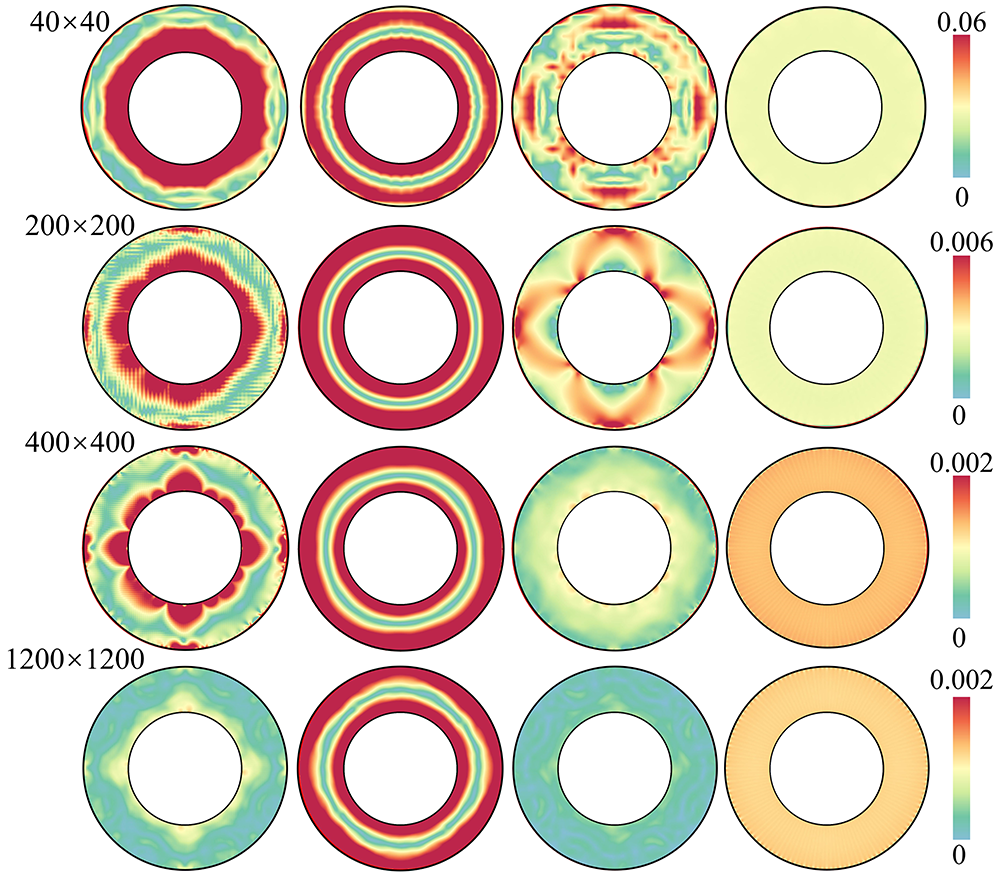
\includegraphics[width=0.99\columnwidth]{figures/taylor-couette-compare-2d.png}
  \bicaption{二维泰勒-库埃特流仿真的对比。我们将不同求解器 (从左至右) 得到的不同分辨率 (从上至下) 的二维泰勒-库埃特流数值仿真结果进行可视化,可视化的值为相对误差,场景设置见图~\ref{img:taylor-couette-setting-2d}。图中从左至右依次为原始的简单反弹边界~\cite{Ladd-1994}、\cite{Li-2020} 中的动理学方法、我们的边界处理,以及ANSYS Fluent求解器。ANSYS Fluent在求解时使用了自适应的体网格,平均元素大小与其它求解器中的网格大小相当。}{Comparison of 2D Taylor-Couette flow simulation. We visualize the relative errors of the numerical solution to the 2D Taylor-Couette flow of Fig.~\ref{img:taylor-couette-setting-2d} computed by different solvers (columns) and different resolutions (rows). From left to right: the original bounce-back scheme~\cite{Ladd-1994}, the kinetic solver of~\cite{Li-2020}, our boundary treatment method, as well as the ANSYS Fluent solver using adaptive radial mesh for which the average element area matches the grid cell area used for the other solvers.}
  \label{img:taylor-couette-compare-2d}
\end{figure}

我们使用了不同的求解器,对该边界驱动的流体进行求解,求解器分别为 (a) 使用原始简单反弹边界~\cite{Ladd-1994} 的动理学方法、(b) DI-IBM~\cite{Li-2020}、(c) 我们的边界处理方法与 (d) 使用N-S方法的商业求解器ANSYS Fluent~\cite{Ansys-2014}。在使用ANSYS Fluent求解时,我们采用了自适应的体网格,平均元素大小与其它求解器中的网格大小相当。由于其使用的是贴体网格,ANSYS Fluent的误差应该会更小。
图~\ref{img:taylor-couette-compare-2d} 展示了不同求解器 (从左至右) 在不同分辨率 (从上至下) 下的相对误差的分布。从图中我们的方法相比其它方法拥有更小误差同时,也随着分辨率上升而更快地达到收敛。

我们还测量了不同求解器结果的加权$\ell_2$误差:
\begin{equation}\label{eq:error_metric}
\epsilon = \frac{\sum_i w(\bm{x}_i)\|\bm{u}(\bm{x}_i)-\bm{u}^{\text{ref}}(\bm{x}_i)\|_2}{\sum_i w(\bm{x}_i)\|\bm{u}^{\text{ref}}(\bm{x}_i)\|_2}\;,
\end{equation}
其中$\bm{x}_i$是流体域中的一个格点,$\bm{u}^{\text{ref}}$是解析解,权重$w(\bm{x}_i) \!=\! 4|r-\bar{r}|$,$\bar{r}\!=\!(r_1+r_2)/2$。这个权重存在的目的是更多地体现边界附近的误差,因为我们本质上在对比边界处理。图~\ref{img:taylor-couette-error-compare} 展示了不同求解器的误差随分辨率上升的变化情况。显然,我们的新边界处理比起其它两个动理学边界处理方法都有着更好的表现。并且,我们的方法在分辨率足够高时,也优于ANSYS Fluent。

\begin{figure}[!htbp]
  \centering
    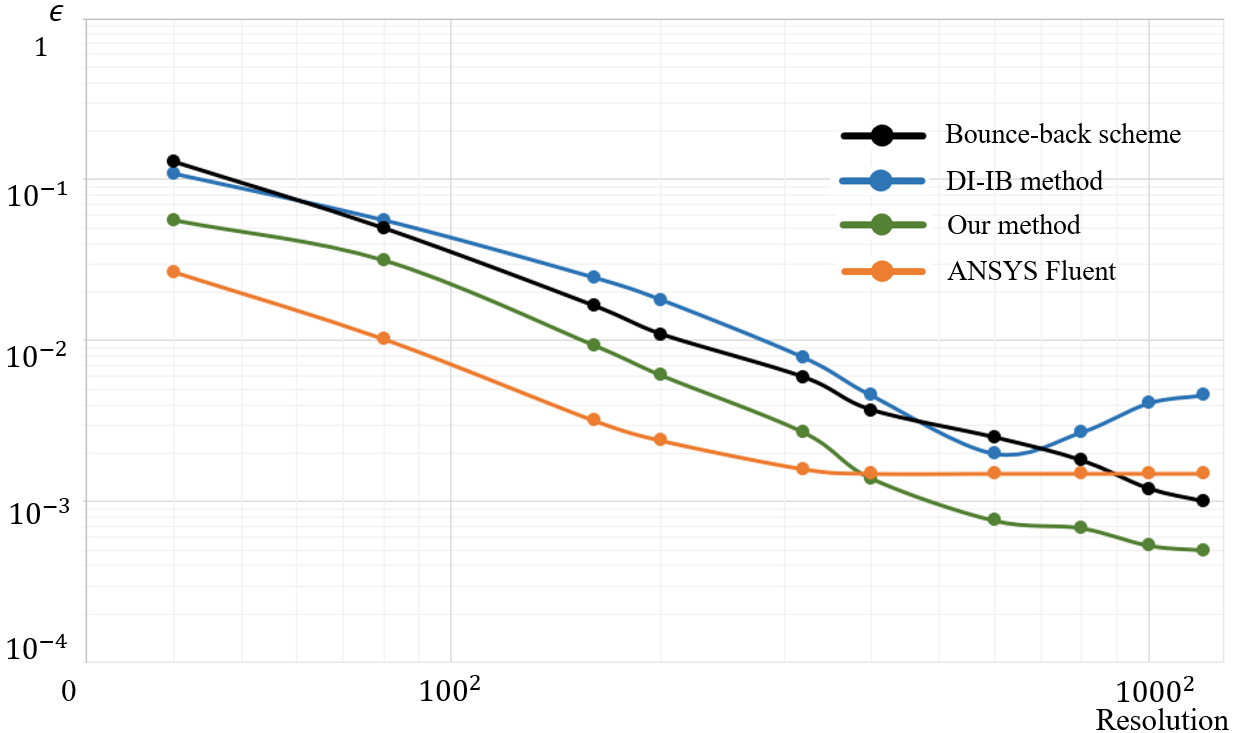
\includegraphics[width=0.94\columnwidth]{figures/taylor-couette-error-compare.png}
  \bicaption{不同类型求解器的误差收敛情况。我们对二维泰勒-库埃特流进行仿真,并衡量了在不同分辨率下,不同类型的求解器的相对误差,以展示各个求解器的误差收敛情况。相对误差根据公式~\ref{eq:error_metric} 计算得到。}{Convergence for different types of solvers. We simulated the 2D Taylor-Couette flows with different types of solvers and measured the relative errors according to Eq.~\ref{eq:error_metric} to show the convergence for different solvers as resolution increases.}
  \label{img:taylor-couette-error-compare}
\end{figure}

\paragraph{与基于切削网格的二维N-S求解器的对比}
CG领域中的N-S方法已经发展得较为成熟,且拥有一系列不同的流固耦合方法。其中基于切削网格的方法是精度与计算效率均相对较高的方法。于是我们与~\cite{Azevedo-2016} 中的基于切削网格的N-S方法进行对比。该方法在切削网格构造了类似有限体积法中的网格以提升精度。我们使用该方法与我们的方法分别仿真了一个二维的薄板以角速度$\omega_s = 3\text{rad}/s$旋转的场景,并将得到的速度场展示在图~\ref{img:cut-cell-based-NS-solver} 中。由于Azevedo等~(\citeyear{Azevedo-2016}) 求解的是无粘度的欧拉方程,我们在我们的方法中也将粘度设为0 ($\nu\!=\!0$)。虽然Azevedo等的方法得到了不错的结果,但是在流场中只有大涡,即使流体本身是无粘的。我们注意到目前也有一些更加精准的N-S求解器,如~\cite{zehnder2018advection,qu2019efficient},但这些方法的计算效率是显著不如动理学方法的~\cite{Li-2020}。从上述分析可得,我们的方法拥有较为独特的优势,即提供了更为精准且高效的湍流仿真,同时可以对不同类型的复杂几何进行耦合。

\begin{figure}[!htbp]
  \centering
    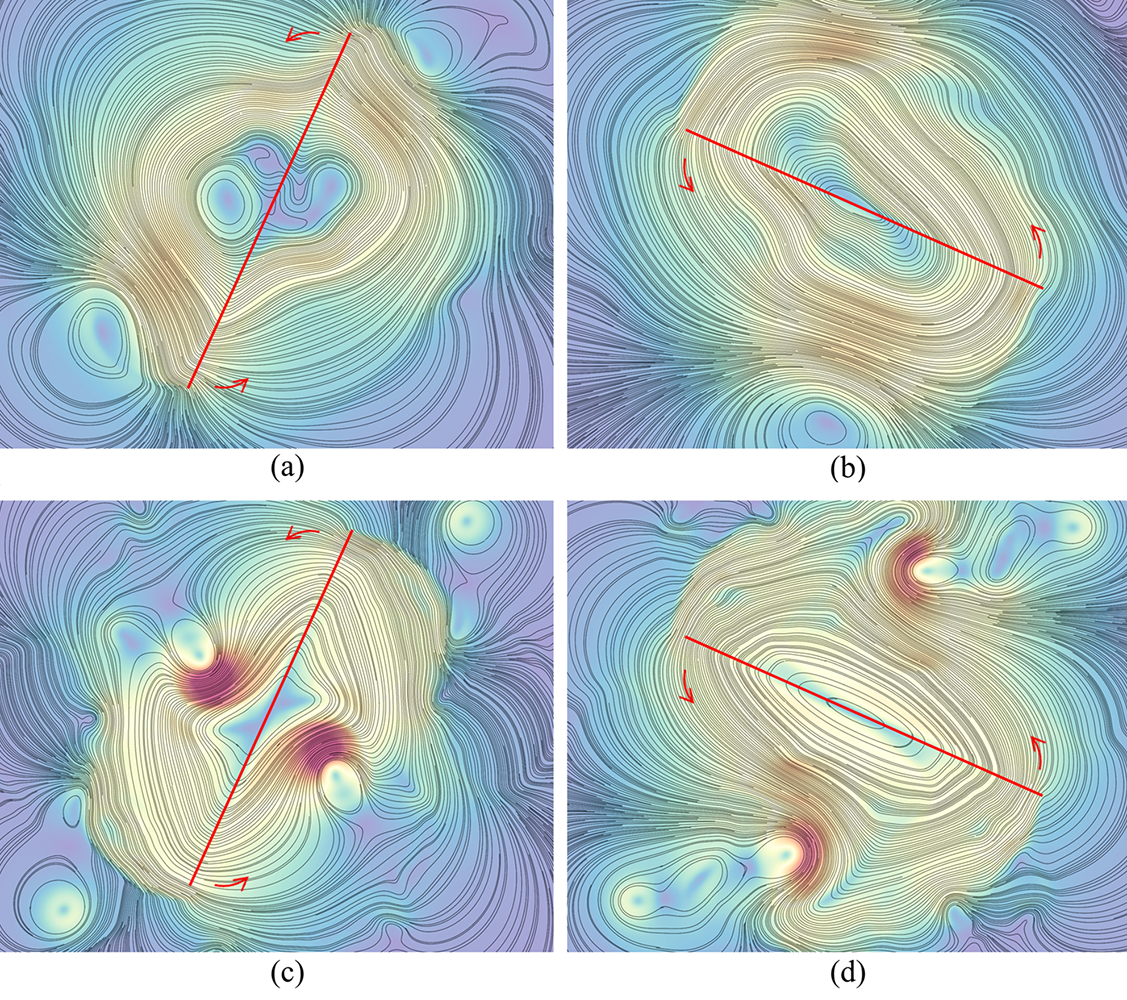
\includegraphics[width=0.99\columnwidth]{figures/ns-compare-2d.png}
  \bicaption{与二维N-S求解器的对比。我们仿真一个二维的薄板在流体中旋转的场景,仿真分辨率为$256\times256$。顶图:由基于切削网格方法的N-S求解器~\cite{Azevedo-2016} 得到的速度场模值;底图:我们的方法获得的速度场模值。(a)、(c) 与 (b)、(d) 分别从仿真中的同一帧截取。虽然两个仿真方法的结果都在视觉上可以接受,但是我们的方法有着更多涡流的细节,证明了我们的方法更适合于湍流的仿真场景。}{Comparison with 2D N-S solver. We simulated a 2D thin plate spinning in a fluid using a grid resolution of $256\times256$. Top: velocity magnitude plot from a cut-cell-based NS solver~\cite{Azevedo-2016}; Bottom: velocity magnitude plot from our solver for the same frames as (a) and (b). Although both solvers retain good boundary velocities, ours produces much more detailed vortices, making it significantly more suitable for solving coupling in a turbulent flow scenario.}
  \label{img:cut-cell-based-NS-solver}
\end{figure}

\subsection{对比}
\begin{figure}[htb]
  \centering
    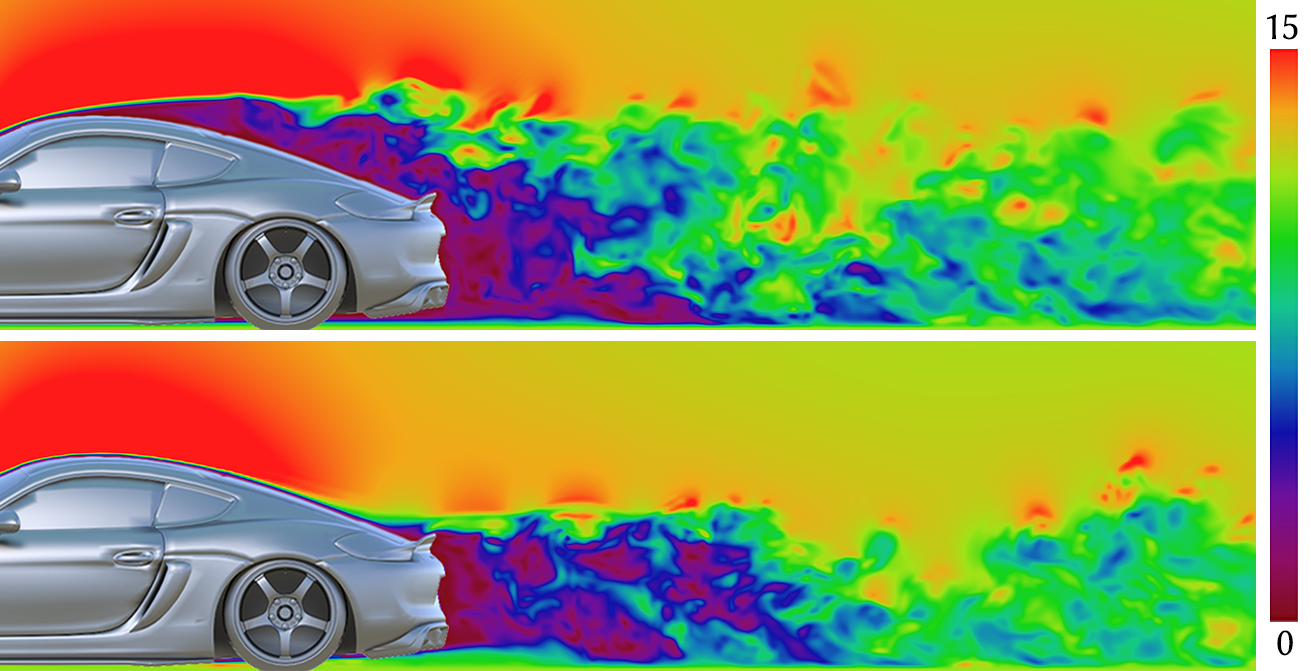
\includegraphics[width=0.99\columnwidth]{figures/comparsion_car_ib_ours.png}
  \bicaption{DI-IBM~\cite{Li-2020} (顶图) 与我们的方法 (底图) 进行气动仿真的对比,速度场截面使用颜色可视化 (单位为$km/h$)。我们的仿真更贴近图~\ref{img:car_wind_tunnel} 中风洞的实际实验,而DI-IBM在车顶即开始发生边界层分离,不切合实际情况。}{Comparison of aerodynamic simulations. DI-IB method~\cite{Li-2020} (top) vs. our result (bottom), using a visualization showing the color-coded velocity field magnitude (in $km/h$) of a cross section. While our simulation matches the wind-tunnel visualization of air flow around a car as Fig.~\ref{img:car_wind_tunnel} demonstrates, the DI-IB method, on the other hand, fails to have accurate boundary treatment, leading to unreasonable boundary layer separation at the top of the car.}
  \label{img:comparsion_car_ib_ours}
\end{figure}

\begin{figure}[!htb]
  \centering
    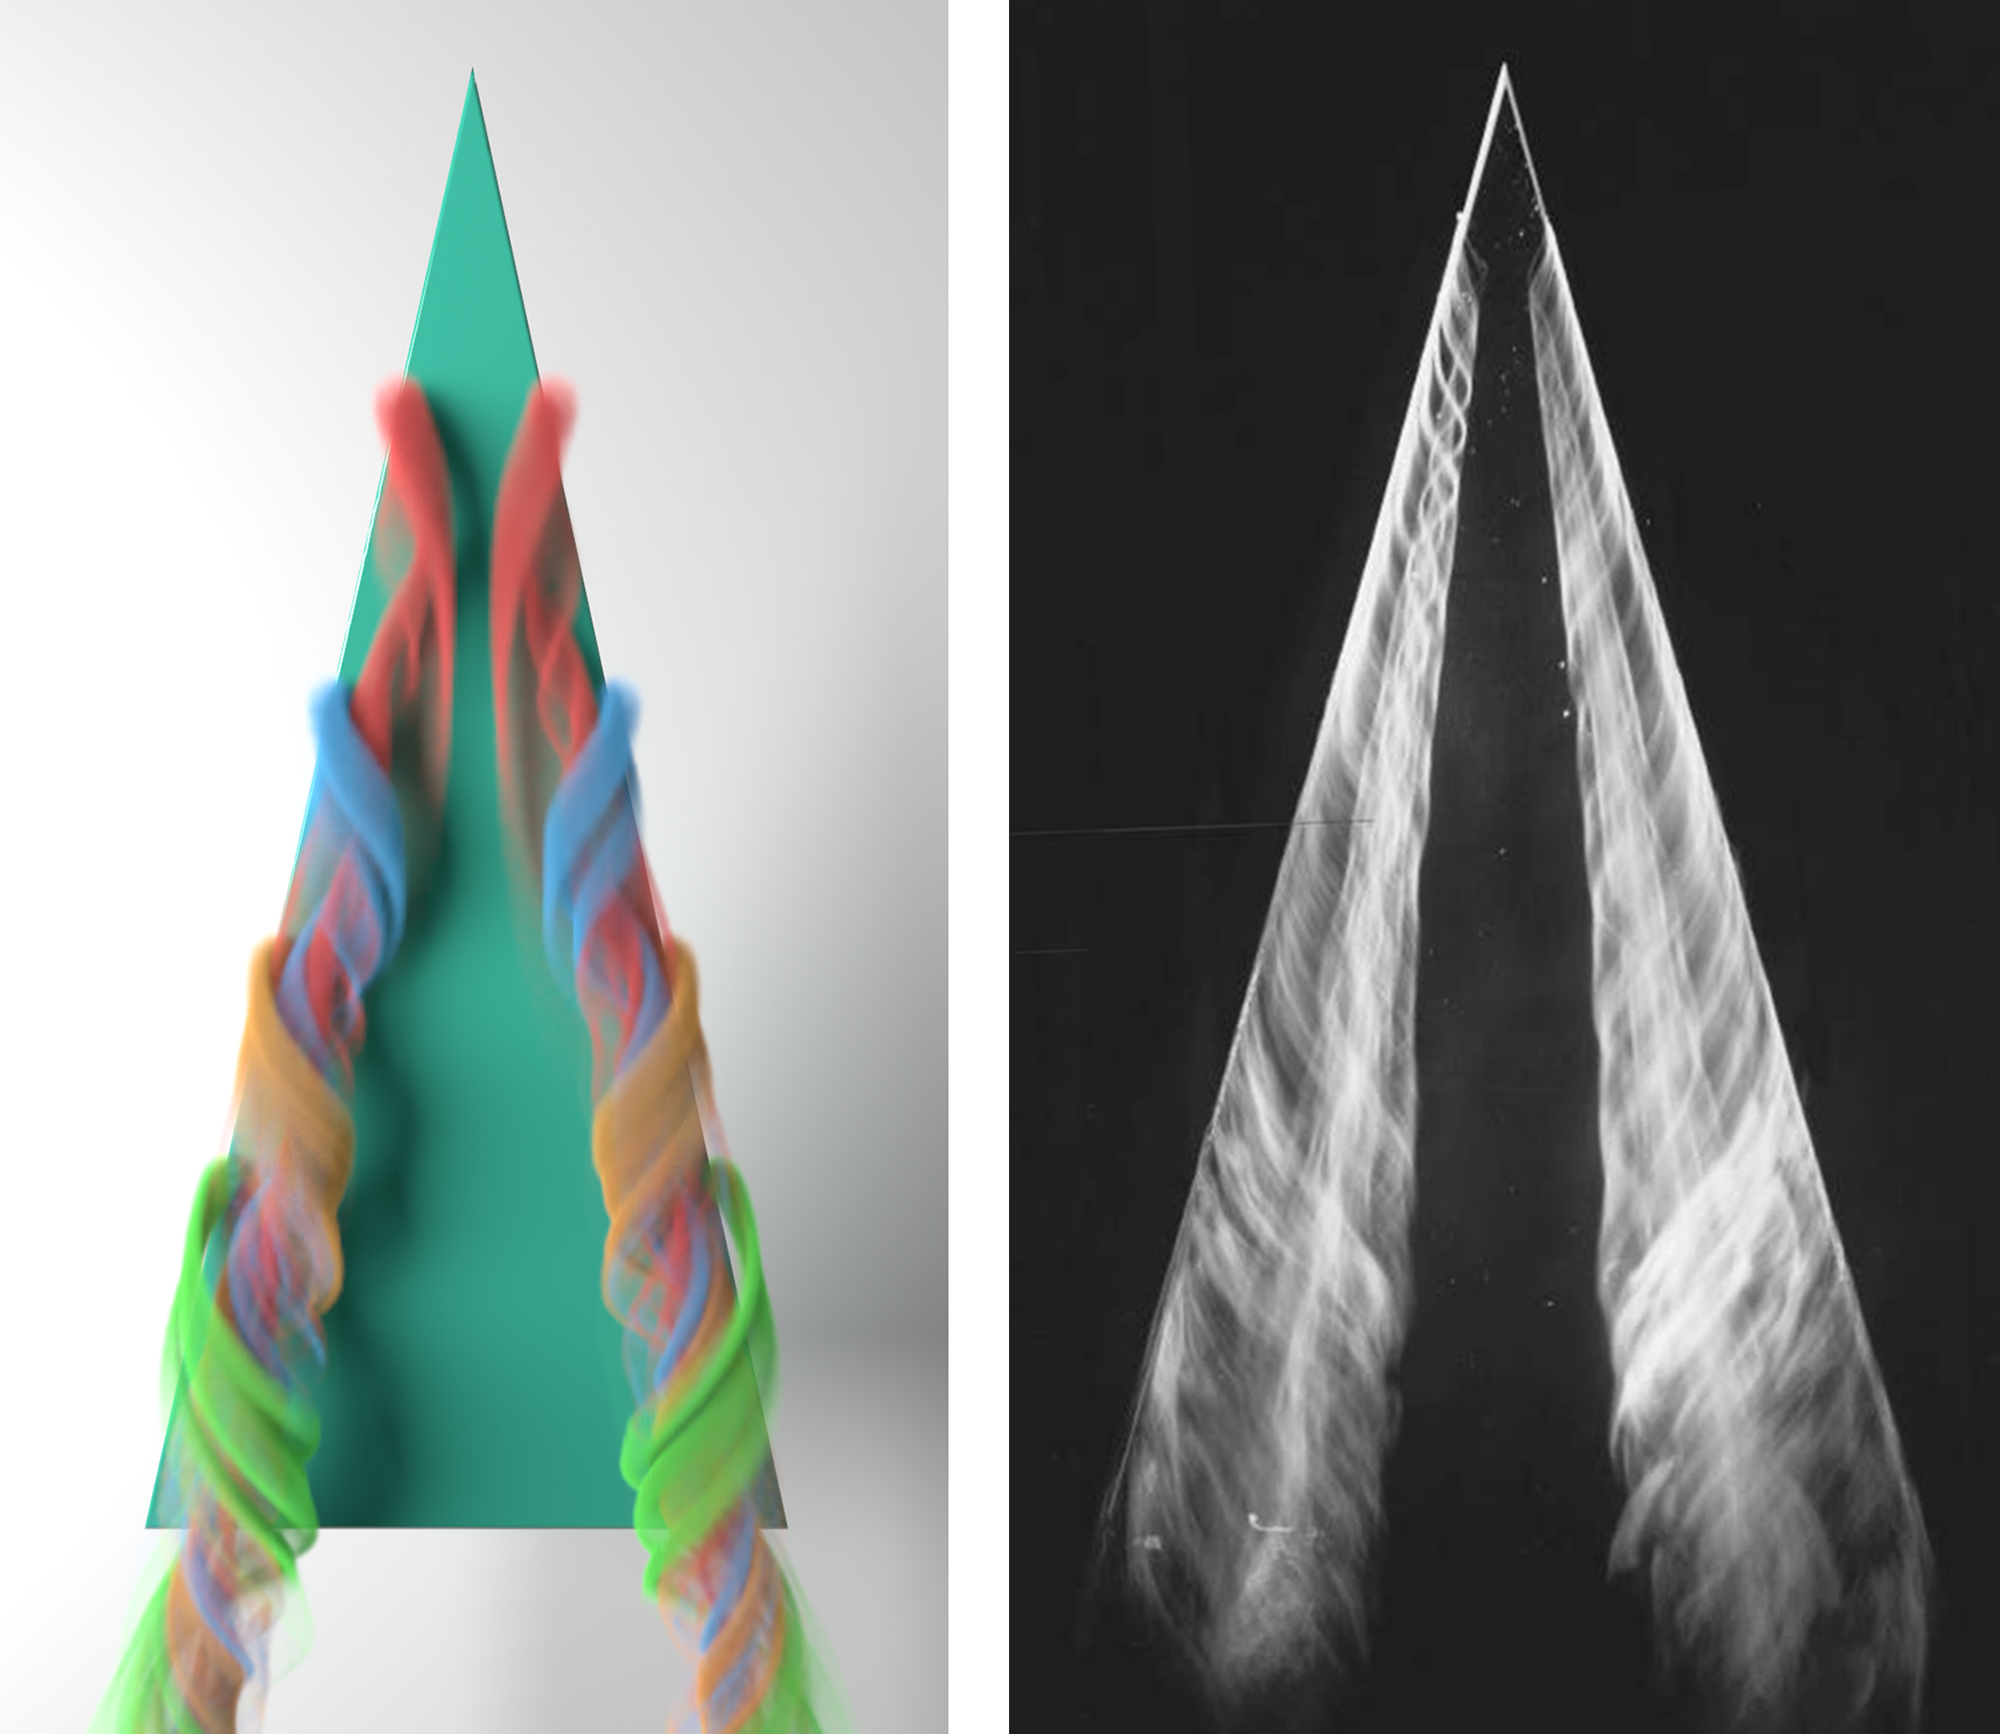
\includegraphics[width=0.99\columnwidth]{figures/comparison_delta_wing.png}
  \bicaption{三角翼仿真。通过我们的方法得到的薄板三角翼仿真结果 (左图) 与实际实验~\cite{Delery:2001} (右图) 的对比,展示出相同的前缘涡旋结构,表面我们的方法在薄结构边界层上的准确性。}{Delta-wing simulation. The airflow over a thin-shell delta-wing simulated with our hybrid coupling approach (left) matches experimental visualizations from~\cite{Delery:2001} (right), exhibiting the same spiral vortex structure near the leading edge of the wing and demonstrating the accuracy of our solver in capturing boundary layer flows around thin structures.}
  \label{img:comparison_delta_wing}
\end{figure}

\paragraph{与图形学中现有方法的对比}
最近,Li等~\citeyear{Li-2020} 提出了一个基于动理学方法的双向流固耦合湍流求解方法,该方法使用DI-IBM处理固体边界。然而这一方法有一定的局限性。首先因为DI-IBM在边界两侧施加惩罚力,其在求解亚网格物体的流固耦合时,会有流体穿透的现象。图~\ref{img:comparison_with_ib} 展示了一个三维的喷射流打向一个薄板,其中图 (a) 使用了Li等~\citeyear{Li-2020} 的方法,并出现了不应该存在的流体穿透现象 (图中红框)。图 (b) 使用了我们的方法,没有产生类似的现象。

另外,DI-IBM有精度不足的问题,使得在湍流仿真时得不到正确结果,尤其是在固体边界层上。我们对一个向前运动的汽车模型进行气流仿真来说明这一问题,见图~\ref{img:comparsion_car_ib_ours}。对于汽车外形来说,气流的分离点一般位于汽车尾部,并且可以通过扰流板等进一步影响尾流走向 (如图~\ref{img:comparsion_car_design} (d) 中的风洞实验)。但仿真结果显示,DI-IBM预测的边界分离点在车顶,完全不符合实际风洞实验,而我们的方法可以正确预测边界的分离点 (两次仿真除边界处理外使用同样的参数设置)。

为了展示如扰流板这样的小且薄的结构对汽车周围流场的影响,我们还在图~\ref{img:comparsion_car_design}中展示了有或无扰流板时汽车流场的仿真结果。从结果中我们可以看到,在添加了扰流板后,汽车的尾流发生了明显的变化。扰流板破坏了车身尾部表面的气流,产生湍流的同时减少了车辆尾部的升力,从而提升了车辆在高速时的操控性。这两个例子展示出了我们的方法针对于计算机图形学中已有LBM方法的优势。

\begin{figure}[!htbp]
  \centering
    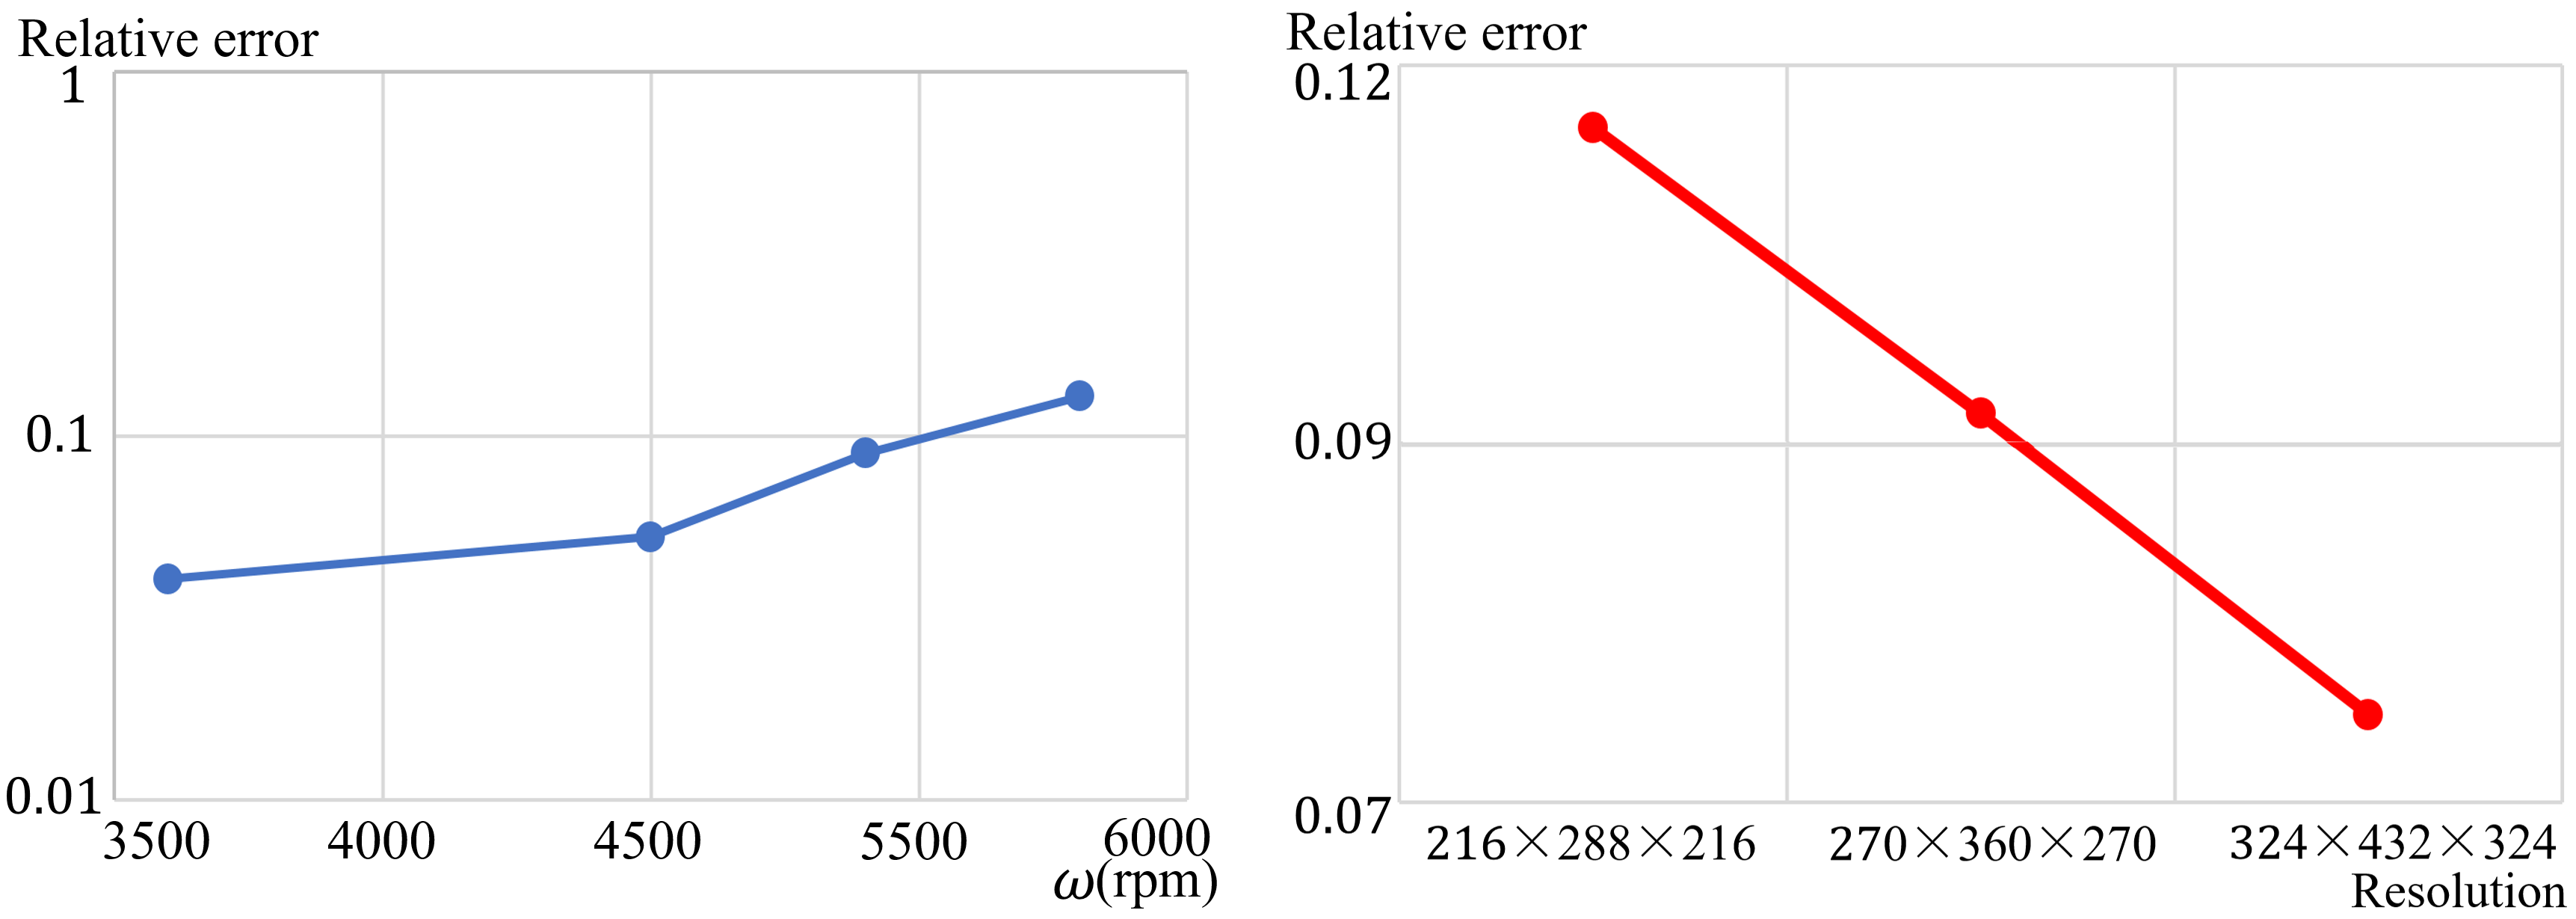
\includegraphics[width=0.99\columnwidth]{figures/DJI_compare.png}
  \bicaption{推力的验证。我们通过旋翼旋转的气动仿真来测试旋翼的推力。我们在$288\!\times\!324\!\times\!288$分辨率下测试不同转速的误差结果见左图。右图为固定3600 rpm转速时,相对误差的收敛情况。注意我们采用的分辨率并不是非常高,所以结果的精度依然有提升空间。}{Thrust evaluation. From the simulation of the coupling between a rotating drone blade and the surrounding air, we can compute the estimated thrust values at different rotation speeds with a grid resolution of $288\!\times\!324\!\times\!288$ (left). The relative errors of our thrust value at 3600 rpm w.r.t. experimental measurements as the grid resolution increases (right) indicates convergence of our solver. Note that the tested grid resolutions are not very high, and more accurate results are expected for higher grid resolutions.}
  \label{img:DJI_thrust_compare}
\end{figure}

\paragraph{与实际实验的对比}
为了进一步验证我们方法在有亚网格物体时边界处理的精度,我们与现实世界中的实验进行对比。
首先我们与三角翼的风洞实验进行比较。该三角翼的后掠角度为$75^\circ$,攻角为$20^\circ$ (见图~\ref{img:comparison_delta_wing} (a))。在实验中,三角翼上方会产生稳定的螺旋涡流结构,提升气动升力 (这种升力被称为涡升力~\cite{anderson2010aircraft})。这种结构被广泛使用于现代飞行器的设计中,如图~\ref{img:teaser_concorde} 中的协和客机。该实验的可视化可见图~\ref{img:comparison_delta_wing} (b)~\cite{Delery:2001}。我们的仿真结果在视觉上与实验结果相匹配,展示出相似的螺旋涡流结构。除去这一定性的对比实验,我们还对旋翼的气动性能进行了定量分析。我们参照一项最近的专利~\cite{lin2020screw} 中的描述重建了旋翼模型,并测量旋翼在旋转时的推力 (计算方法参照~\cite{leishman_2016}),与专利中的数据对比。图~\ref{img:DJI_thrust_compare} (a) 展示了不同转速下的计算误差,显示出较好的一致性。值得注意的是,随着转速的提升,相对误差会升高。这一点的主要原因是在LBM中,随着参照速度的提升,LBM空间下粘度在不断减小,以至于我们在测试时使用的32位浮点数已无法有效保证碰撞过程的计算精度。我们还对收敛性进行了测试,即在固定转速下提升分辨率,结果可见图~\ref{img:DJI_thrust_compare} (b)。这一结果显示了我们方法误差随分辨率的收敛性。

\begin{figure}[!htbp]
  \centering
    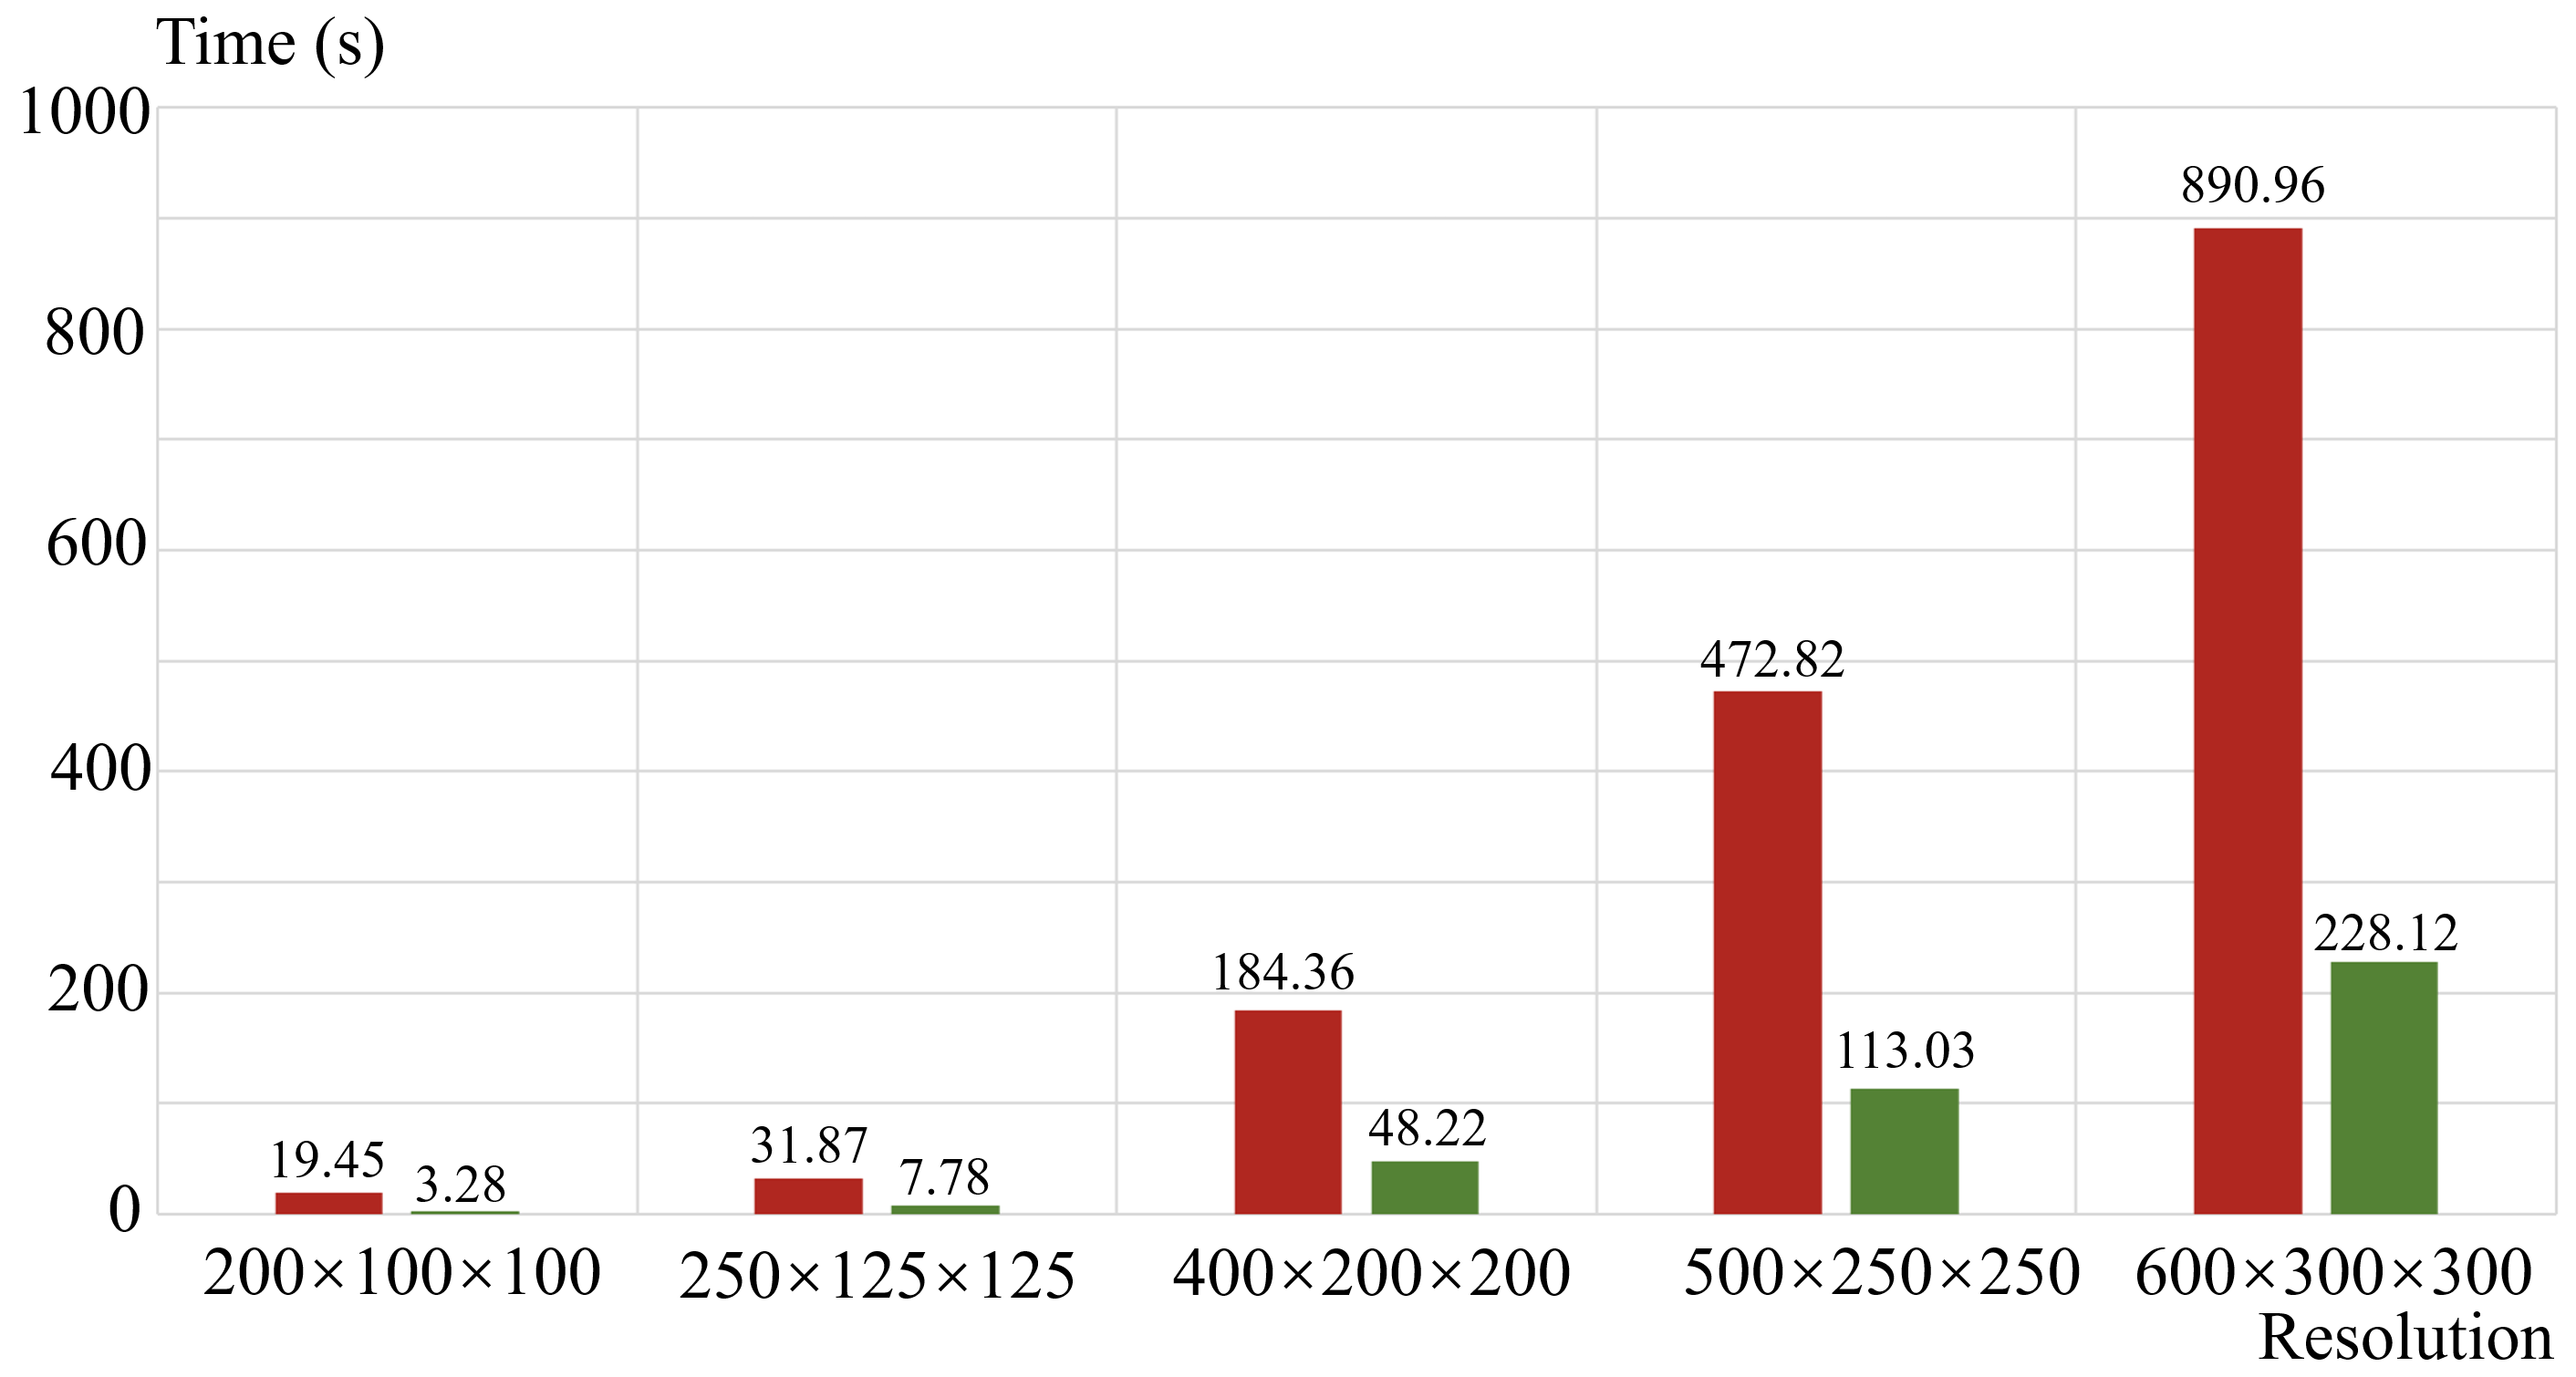
\includegraphics[width=0.93\columnwidth]{figures/performance.png}
  \bicaption{性能对比。我们将我们的方法 (绿色) 与Li等~(\citeyear{Li-2020})、Chen等~(\citeyear{Chen-2021}) 中的动理学求解方法 (红色) 进行比较,比较用例为图~\ref{img:comparsion_car_ib_ours} 中所示的汽车仿真,仿真时长为1秒。在同一张NVIDIA RTX 3090 GPU上得到的测试结果显示我们的方法在所有分辨率上都有显著的性能提升。}{Performance comparison. We compare the efficiency of the kinetic solver from~\cite{Li-2020,Chen-2021} (red) with our kinetic solver (green) based on one second of simulation of the car model shown in Fig.~\ref{img:comparsion_car_ib_ours} and both executed on a same NVIDIA RTX 3090 GPU, showing significant performance improvement for all grid resolutions.}
  \label{img:Performance}
\end{figure}

\paragraph{性能对比}
在Li等~(\citeyear{Li-2020}) 与Chen等~(\citeyear{Chen-2021}) 中,作者已经通过对比,说明了动理学方法的计算效率是显著优于N-S方法的。这种优势在湍流流固耦合仿真中更加明显,因为需要的时间步长更小。由于我们的方法与这些工作的框架相同,结合上述的各项优化,使得我们的方法在性能上更有优势。我们在同一张NVIDIA RTX 3090 GPU上,进行了多个分辨率的对比,结果显示我们的方法在所有的分辨率上都有显著提升 (见图~\ref{img:Performance})。通过代码性能分析,我们分析出两个使性能得以提升的主要因素:第一个是基于LU分解的碰撞运算符简化~\cite{fei2018three} 显著提升了GPU占用率,第二个是使用了几何近似优化之后,我们的混合边界处理比起之前工作使用的DI-IBM,计算量要更小。这两点使得我们的GPU计算效率得以提升。

\subsection{仿真结果}
下面我们展示一系列的仿真结果。这些仿真结果都于一个14核Intel Xeon E5-2690 CPU、128 GB内存、NVIDIA RTX 3090的工作站上运行得到。我们通过一系列的单向与双向流固耦合算例,对一系列的复杂几何进行测试,以显示我们的方法处理不同类型物体的能力。我们还展示了一些可交互的仿真、与离线的高分辨率大规模仿真。

\begin{figure}[!htbp]
  \centering
    \includegraphics[width=0.99\columnwidth]{figures/result_tube.png}
  \bicaption{旋转的薄圆柱面。一个薄圆柱面分别在高粘度 (顶图) 与低粘度 (底图) 流体中绕轴旋转。在圆柱面内部和外部分别有烟雾粒子对流场进行可视化 (内部为蓝色,外部为红色)。左图与右图分别展示仿真在4s与7s后的烟雾形态。}{Rotating cylindrical thin shell. A cylindrical thin shell rotating around its axis in a very high (top) and very low viscosity (bottom) fluid respectively, where smoke particles scattered inside (blue) and outside (red) the thin-shell cylinder are advected in the flow (left: after 4 seconds; right: after 7 seconds) to demonstrate that boundary layers are well resolved.}
  \label{img:result-tube}
\end{figure}

\begin{figure}[!htbp]
  \centering
    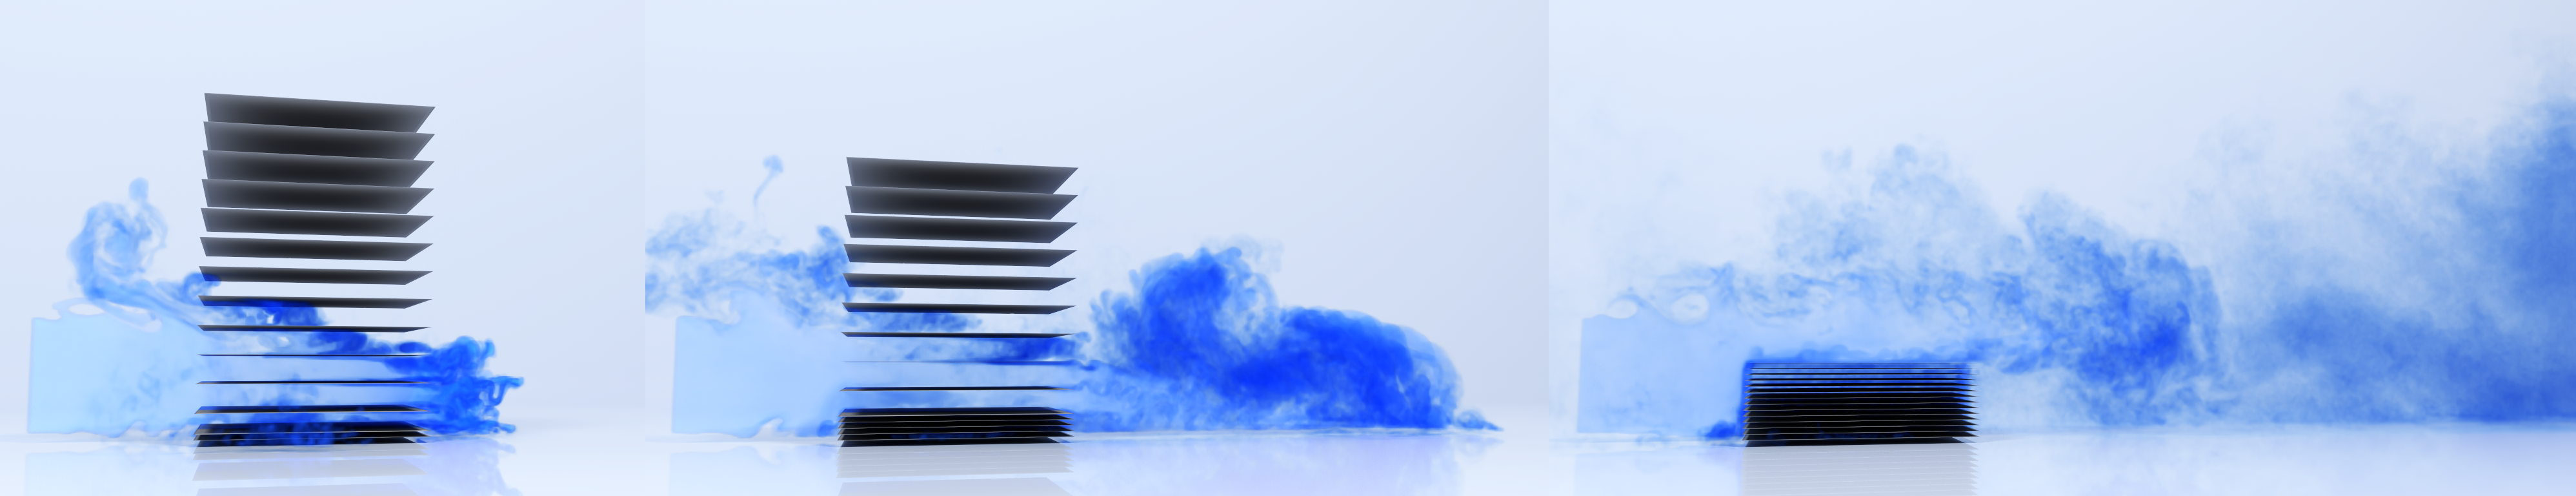
\includegraphics[width=0.99\columnwidth]{figures/result_thin_shell_sub_grid.png}
  \bicaption{烟雾经过层叠的板子。烟雾吹过一系列下落的薄板。虽然薄板在分开时烟雾可以通过,当它们层叠在一起时却形成一个密闭的障碍物。我们边界处理中的亚网格近似可以同时处理这两种不同情况,当板子加速靠近时,中间的流体会被加速,而它们紧贴时会成为一个厚的物体。}{Smoke flow through stacked plates. Smoke is blown towards a falling stack of thin plates. While smoke freely flows between separate plates, they become an airtight obstacle when they are stacked on top of each other. Our boundary treatment based on subgrid approximation deals with both cases seamlessly: plates getting closer accelerate the flow in between them, while tightly stacked plates are treated as thick solids.}
  \label{img:result-thin-shell-sub-grid}
\end{figure}

\begin{figure}[!htbp]
  \centering
    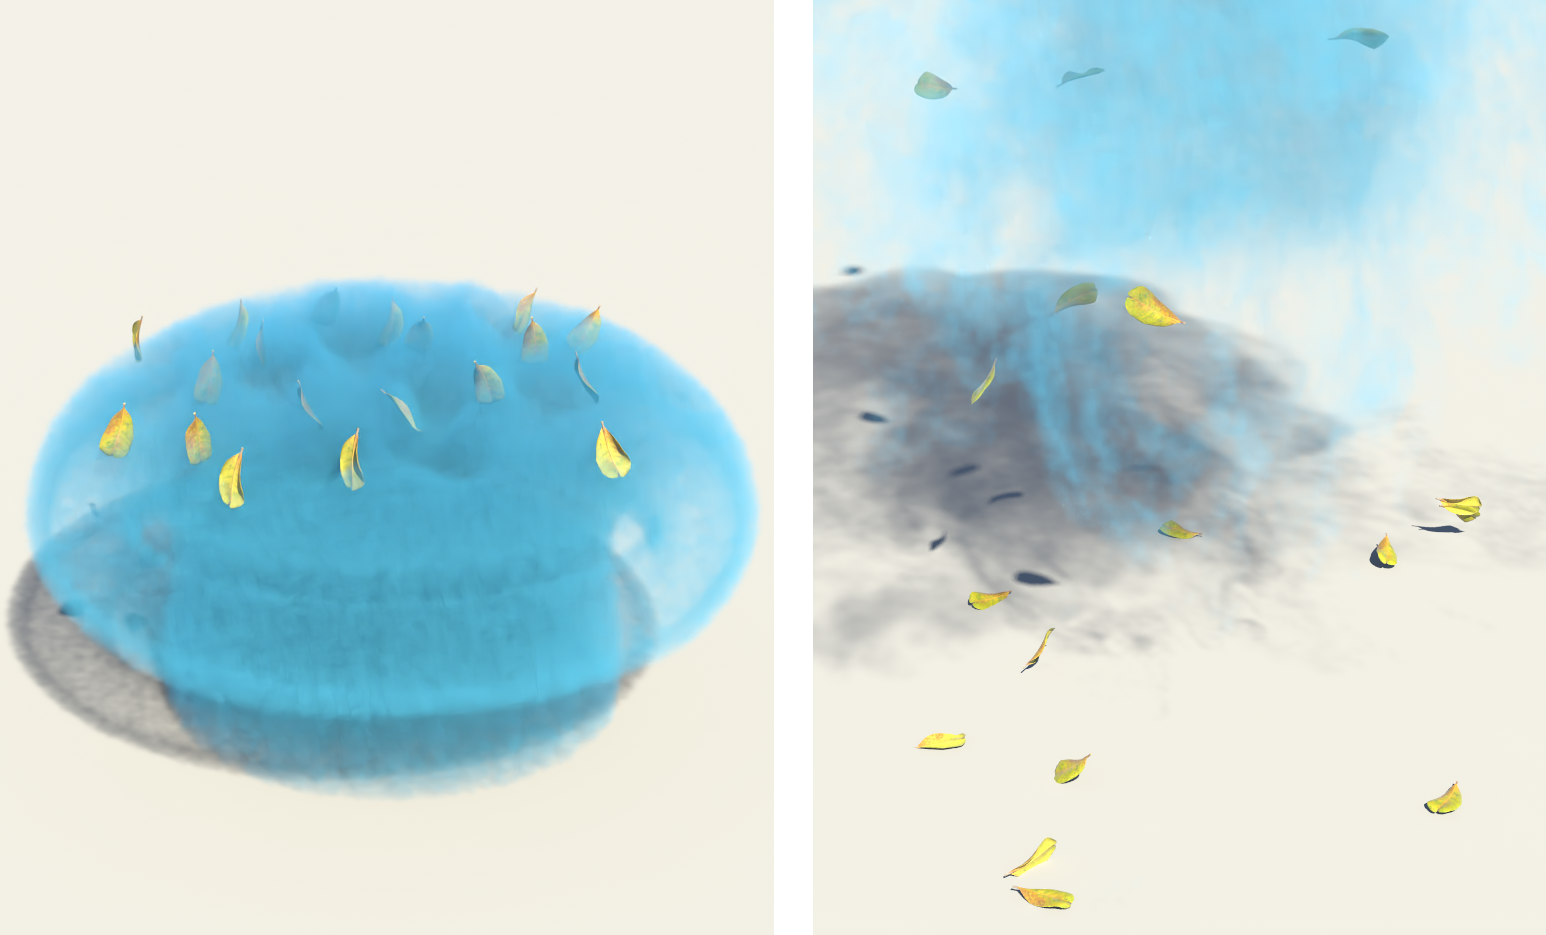
\includegraphics[width=0.99\columnwidth]{figures/result_blowing_leaves.png}
  \bicaption{风吹叶子的仿真。在这个双向流固耦合结果中,一阵风从地面吹起将树叶吹向空中。}{Wind blowing leaves. In this two-way coupling example, a puff of wind from the ground drives a bunch of dried-up leaves up in the air.}
  \label{img:result-blowing-leaves}
\end{figure}

\paragraph{与薄板的耦合}
我们首先构造一个薄圆柱面,使得厚度远小于网格大小,之后令圆柱面旋转,产生剪切流 (见图~\ref{img:result-tube})。我们在低雷诺数 (高粘度) 与高雷诺数 (低粘度) 分别进行了测试,并展示出完全不同的流场特性。我们还测试了多个薄板相叠的算例。这些薄板最初是分开的,之后逐渐叠落在一起。我们的亚网格近似使得我们的方法可以仿真从起初分离的薄板到叠在形成一个固体的整个过程,而无需任何调整。结果可见图~\ref{img:result-thin-shell-sub-grid}。我们最后展示一个双向耦合的结果,仿真一阵风从地面吹起树叶的过程。树叶一开始被风吹起后,缓慢地落回地面,并因风产生旋转。结果可见图~\ref{img:result-blowing-leaves}。

\begin{figure}[!htbp]
  \centering
    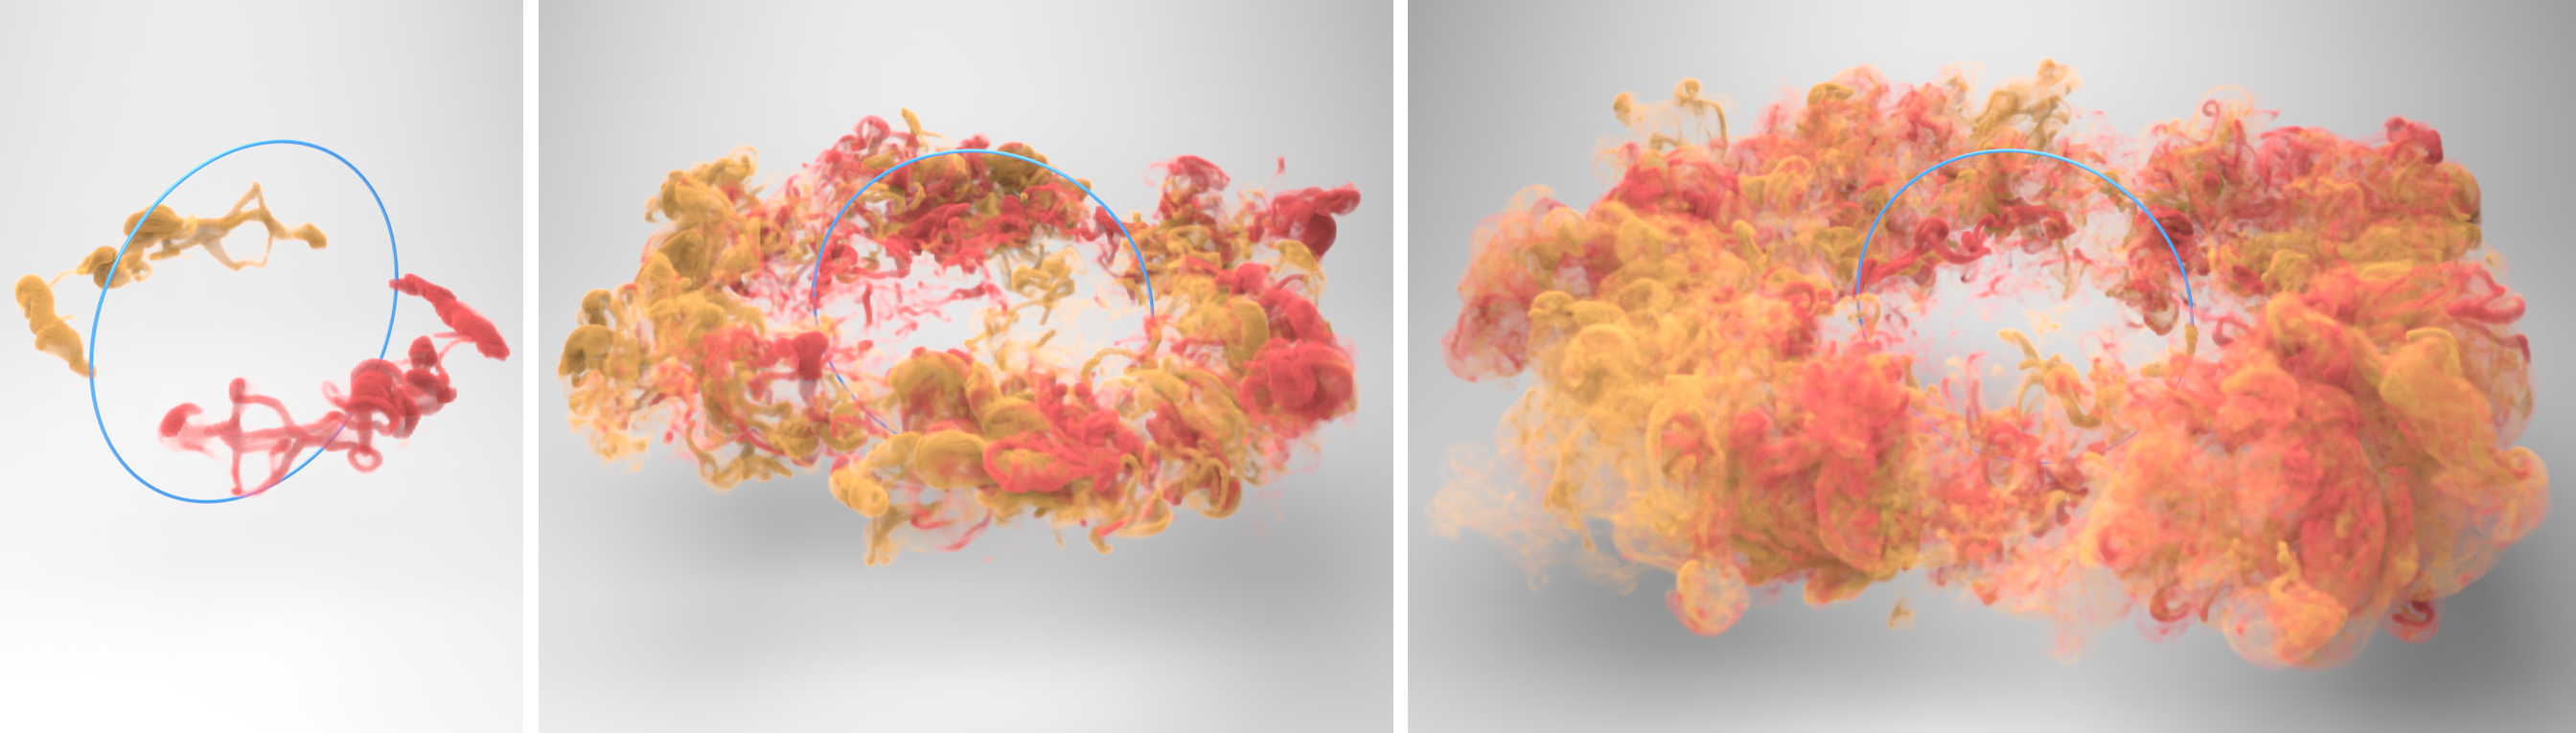
\includegraphics[width=0.99\columnwidth]{figures/result_rotating_torus.png}
  \bicaption{旋转的圆环。一个非常细的圆环沿着一个垂直轴旋转,在两侧发出黄色和橘色的烟雾,展示出圆环旋转所带出的湍流。}{Rotating ring. A very thin ring rotating along a vertical axis and emitting yellow and orange smoke particles is enough to create a turbulent wake as evidenced by the volutes of smoke resulting from the motion.}
  \label{img:result-rotating-torus}
\end{figure}

\begin{figure}[!htbp]
  \centering
    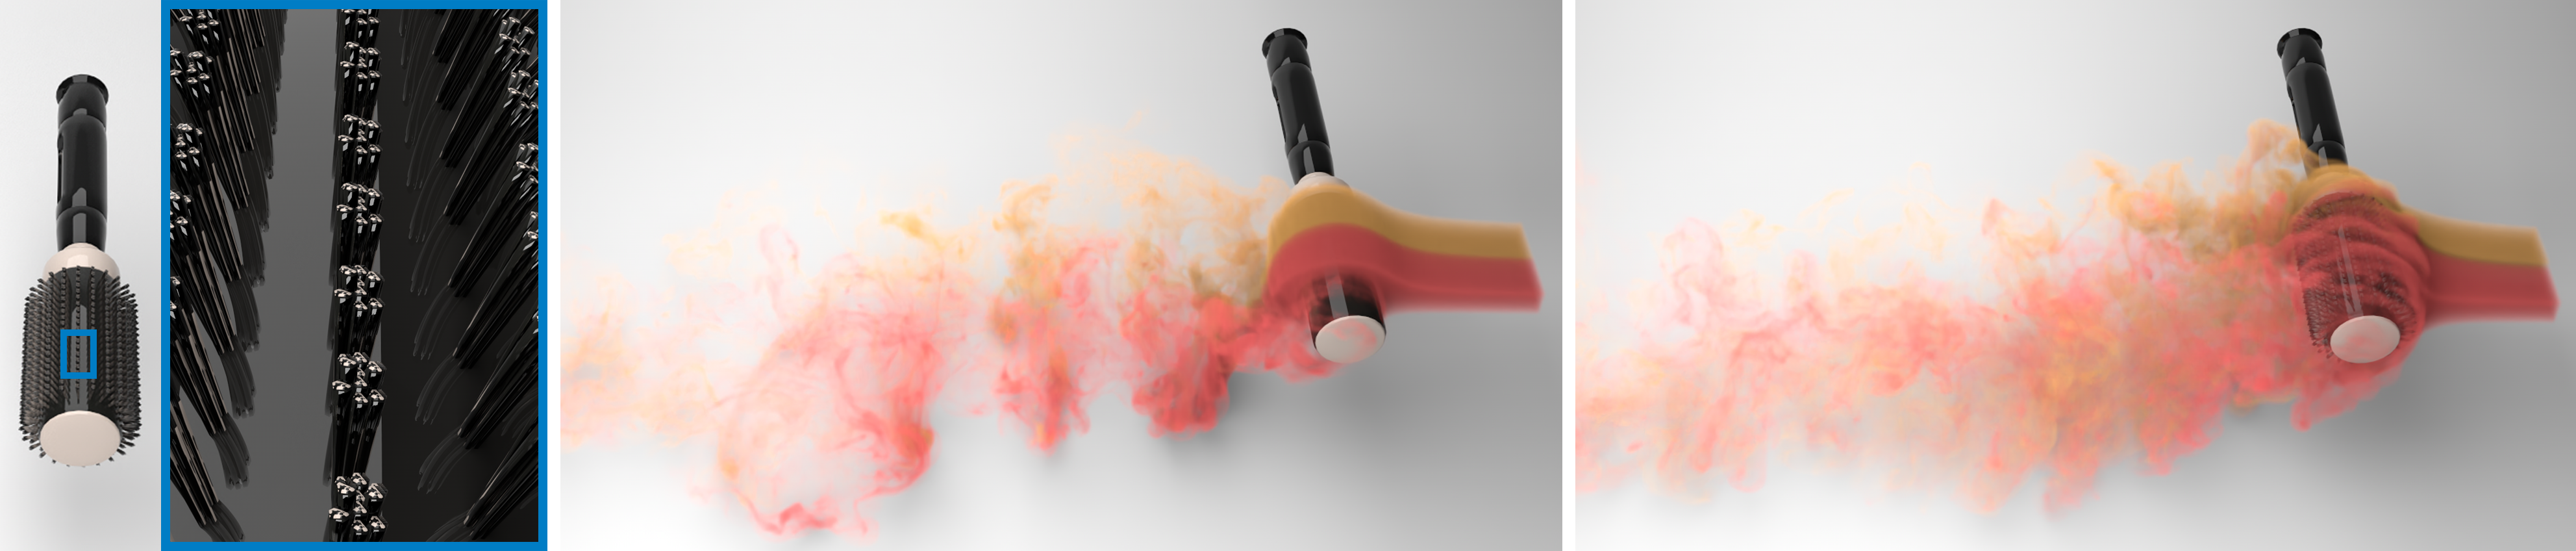
\includegraphics[width=0.99\columnwidth]{figures/result_thin_rod_sub_grid.png}
  \bicaption{发梳仿真。一个包含着上百根硬毛地发梳 (左图) 在旋转的同时从左向右平移,带动周围气流运动。与有硬毛的情况 (右图) 相比,没有硬毛时的发梳 (中图) 运动产生的尾流更加平滑,涡旋也更大。这个结果展示了我们的边界处理方法,包括亚网格近似,处理复杂几何的能力。}{Hair brush. The translating and rotating motion of a hair brush containing hundreds of bristles (left) creates fine vortices in its wake as well as around the bristles (right) as evidenced by the evolution of the smoke passing around it, properly capturing the intricate fluid-solid interaction engendered by this complex geometry. Compared to the coupling with bristles (right), the smoke near the hair brush without bristles (middle) is much smoother, and the wake flows contain relatively large vortices, indicating the efficacy of subgrid approximation in handling such complex solid shapes.}
  \label{img:result-thin-rod-sub-grid}
\end{figure}

\paragraph{与细棒的耦合}
下面继续展示我们的求解器对细棒耦合的仿真结果。我们先展示一个环状物体在空气中定速旋转的结果,其直径远小于网格大小,见图~\ref{img:result-rotating-torus}。我们还对多个细棒组合在一起时的情况进行仿真,结果见图~\ref{img:result-thin-rod-sub-grid}。注意当固体表面有硬毛时,尾流的湍流程度有显著的差别。

\begin{figure}[!htbp]
  \centering
    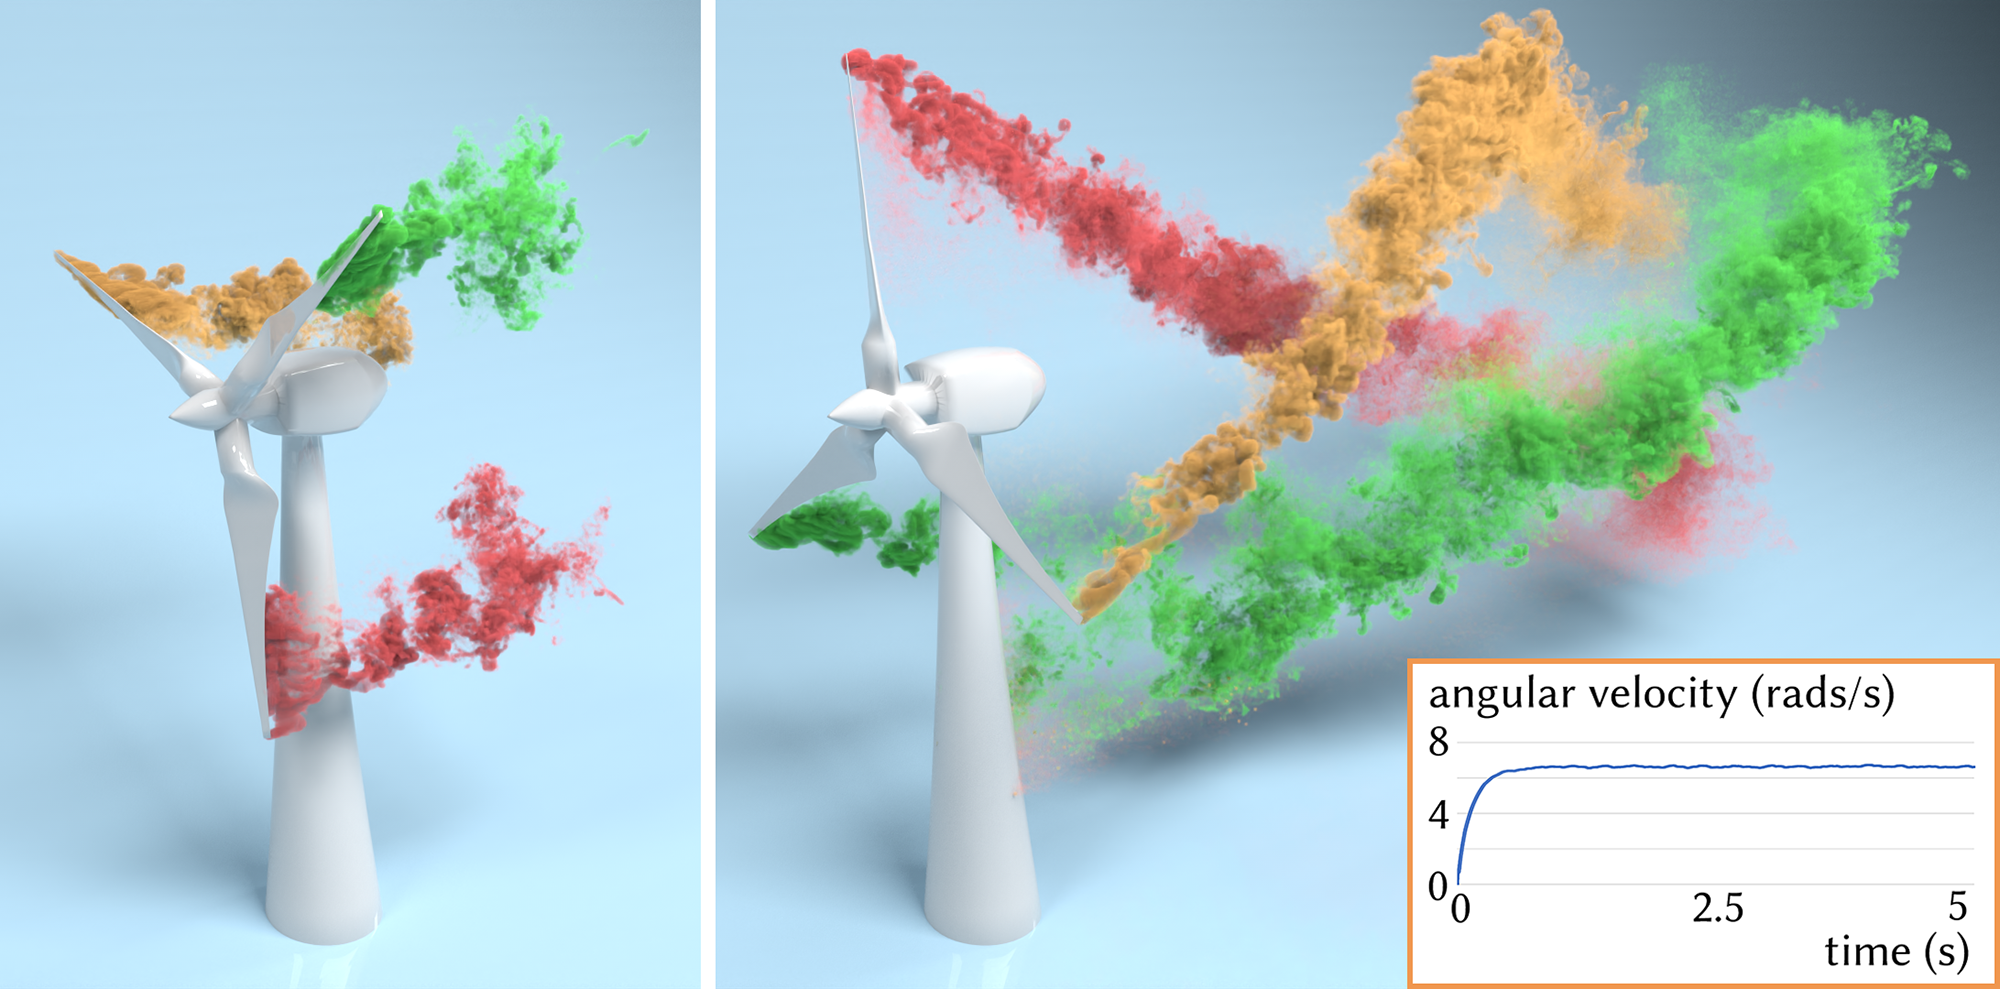
\includegraphics[width=0.99\columnwidth]{figures/result_wind_turbine.png}
  \bicaption{风力涡轮机的仿真。常速的风吹过一个有三个扇叶的风力涡轮机,驱动涡轮机旋转,并由扇叶上产生的烟雾对涡旋尾流结构进行可视化。这个双向的流固耦合结果考虑了轴上的摩擦力来限制了最大的角速度。扇叶角速度随时间的变化可见底部的小图。}{Turbine. A large turbine emitting colored smoke particles at the three propellers of its large blade is simulated with a constant incoming air flow making it turn, creating a spiral vortex trail. This two-way coupling example also involves friction on the axis of the turbine to limit its maximum angular velocity, resulting in a time-varying but converging curve of angular velocity of the turbine shown in the bottom inset.}
  \label{img:result-wind-turbine}
\end{figure}

\begin{figure}[!htbp]
  \centering
    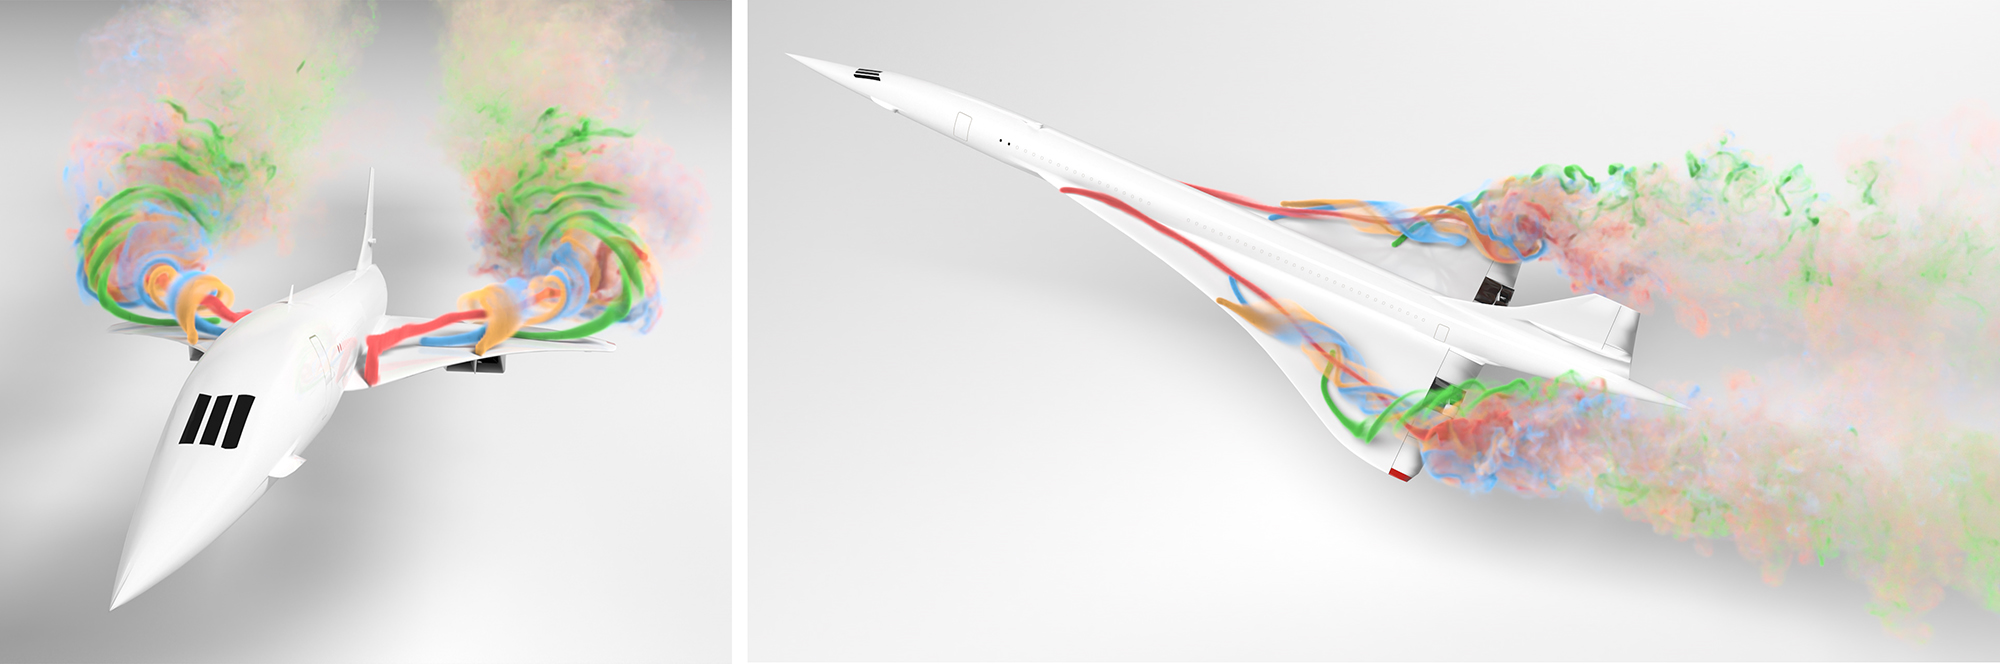
\includegraphics[width=0.99\columnwidth]{figures/teaser_concorde.jpg}
  \bicaption{飞机气动仿真。通过对协和客机翼面的气流仿真,我们展示出我们的方法可以同时处理含有薄板、细棒的薄物体以及厚物体的复杂几何。}{Aerodynamic simulation of an airplane. By simulting the flow over the wing of the Concorde airplane, we demonstrate that our method can handle complex solids containing thin shells, rods and thick objects.}
  \label{img:teaser_concorde}
\end{figure}

\paragraph{与复杂物体耦合}
一个更复杂但非常常见的情况是厚物体与薄物体同时存在,并共同构成一个复杂物体。我们的边界处理可以有效并统一地处理这种情况。图~\ref{img:result-wind-turbine} 展示了通过风带动一个三扇叶风力涡轮机模型旋转的仿真结果。这里风在带动扇叶旋转的同时,扇叶也影响空气流动,展现了我们方法处理复杂物体的双向耦合。图~\ref{img:teaser_concorde} 展示了协和式客机以攻角20度姿态在空中飞行的仿真结果。对于飞机这样的复杂物体,许多部件对于网格都是亚网格大小的,尤其是机翼部分。在这两次仿真中,得到的结果都与期望相符。

\begin{figure}[!htbp]
  \centering
    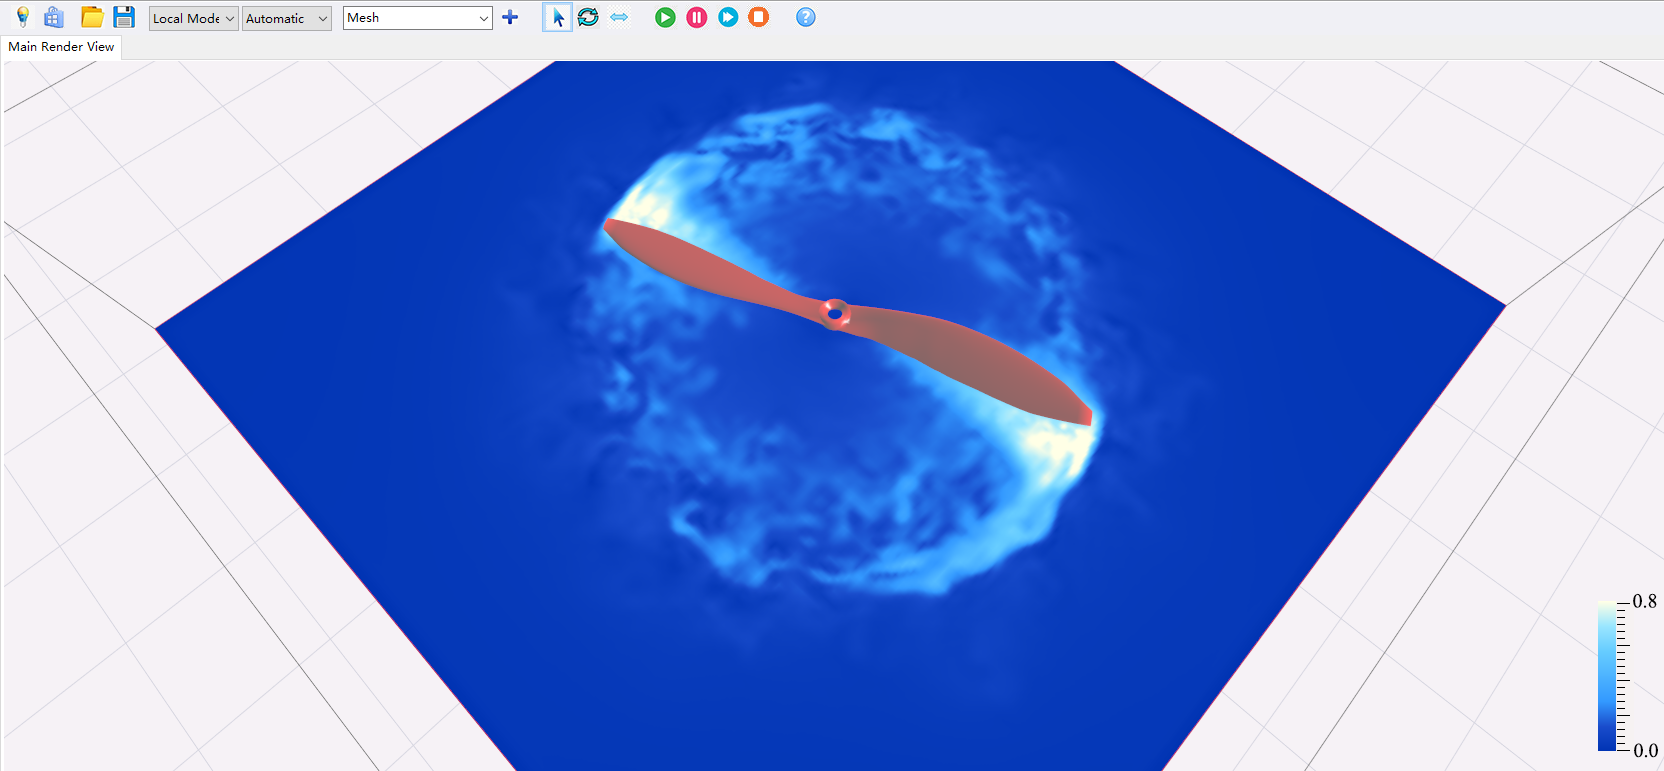
\includegraphics[width=0.99\columnwidth]{figures/result_design.png}
  \bicaption{快速交互设计。我们通过GUI操作模拟系统,来快速生成仿真结果。图中示例为一个快速旋转的旋翼,我们可以通过可视化即时的看到尾流情况。这样的快速交互式仿真可以用来辅助产品设计与验证。}{Fast simulation for interactive design. We operated our GUI-based simulation system to produce a quick preliminary result of a fast rotating rotor-blade where turbulent wake flows can be observed interactively, which is very useful for efficient product design and verification.}
  \label{img:result-design}
\end{figure}

\paragraph{快速仿真以进行交互式设计}
我们的流固耦合算法可足够高效,以进行交互式产品设计与测试。作为示例,我们在$200\!\times\!200\!\times\!200$分辨率下对一个旋翼旋转的情况进行仿真。图~\ref{img:result-design} 展示了仿真中的速度场截面。完成1/100 s的仿真所需的计算时间为0.4 s。这个时间包括数据的读取与可视化 (截面可视化在CPU上完成)。这意味着类似旋翼这类的产品可以使用我们的算法进行快速的气动性能评估,并可基于此优化设计。

\begin{figure}[!htbp]
  \centering
    \includegraphics[width=0.99\columnwidth]{figures/result_city.png}
  \bicaption{气流经过城市街区的高分辨率仿真。我们对气流经过城市街区进行高分辨率仿真 (($889\times333\times556$)),建筑中包含诸多细且尖锐的结构。一层相对薄的烟雾从左侧注入,在建筑间产生涡流细节。}{High-resolution simulation of airflow through a city neighborhood. We simulate the airflow passing around and over buildings using a high resolution grid ($889\times333\times556$), where the buildings contain both thin and sharp structures. A layer of smoke particles with relatively small thickness is coming from the left, creating fine vortical structures behind and in between the buildings.}
  \label{img:result-city}
\end{figure}

\paragraph{高分辨率仿真}
最后,我们展示一个高分辨率的大规模仿真结果,来展示我们方法的可扩展性。该仿真使用两个GPU同时计算,展示了大量烟雾穿过一个高密度城市街区的场景 (见图~\ref{img:result-city})。场景中包含诸多细且尖锐的物体对尾流产生影响。对于这样的大场景湍流仿真,5 s的仿真所需的计算时间为1.5小时左右。正如Li等~(\citeyear{Li-2020}) 所讨论的,达到这样的仿真效率对于N-S方法来说是十分困难的,即使同样使用多GPU进行加速。主要原是N-S方法中压力场求解这一步需要求解全局的线性方程组,在高分辨率下会严重影响计算效率。

\section{方法的局限性}
虽然我们的方法展示出了优秀的通用性与数值结果,我们的方法依旧有一定的局限性。
首先,由于我们使用了基于采样点的几何计算近似,当固体包含尖角的时候,是否需要应用反弹边界可能发生误判。增加采样点数量或使用自适应采样可以提升精度,但是也会同时提升显存需求。第二,对固体所受的力和力矩的计算也受制于对固体外形的近似。如我们的亚网格近似无法真实反应物体的几何形状,会影响固体受力计算的精度。最后,对于可变形的物体,我们的方法需求一个更高效的采样方法,以每帧更新物体表面的采样点。

\section{总结}
在本章中,我们提出了一个基于动理学方法的混合边界处理方法,以处理在流固双向耦合。我们的方法可以有效、统一地同时处理厚、薄物体,并可以稳定、快速地完成仿真,得到视觉上可信的结果。我们的方法充分利用了反弹边界与尖锐界面浸没边界法优点的互补性,包含双面反弹边界处理与单边的速度修正,与双向耦合所需的固体受力计算。
我们基于边界采样点提出了高效的几何近似算法与对应的GPU并行实现,以提升整体计算效率。我们的方法在效率与精度上都超越了现有的计算机图形学中的LBM算法,并在强湍流中依然可以捕捉到正确的物理现象。
我们展示了我们的方法与其它方法和实际实验的对比,和一系列的仿真结果,包括不同的几何形状在流体中的单向或双向耦合仿真,及我们的方法在快速交互式设计中的应用。
\chapter{更加通用的高精度流体仿真方法}
\label{chap:sig23}

我们在上一章中已经描述了应用于视觉动画的LBM方法,但是对于工业应用来说,以上的方法并不能满足要求。其中有几个原因。第一个原因是,第~\ref{chap:siga21} 章所描述的混合方法虽然高效,但以真实世界中的风洞举例,在真实的风洞实验中,物体周围的边界层已经非常薄,远小于网格大小,从而在网格层面假设速度是线性的已经不够精确。第二,在这样的尺度下,我们已经无法单纯地依靠提高分辨率,以解决这一问题,而必须依赖于多分辨率网格,在上一章中的方法并没有涉及相关的处理。第三,对于工业应用,碰撞模型等LBM的核心算法,对结果也有着至关重要的影响,而这一点在上一章中也未有足够的讨论。所以在这一章中我们将介绍一个更加通用的高精度流体仿真方法,并更专注于一些实际工业产品设计与验证等应用。更具体地,我们尝试将现实中工业产品设计中非常常见的风洞实验,通过流体仿真的形式数字化。所以在下文中,我们也可将本章中描述的方法称为基于LBM的虚拟风洞测试系统。这个目标使我们不只局限于边界处理等方法本身,还需要整体的仿真框架配合。从而在本章中,我们将更为整体地描述整个仿真框架。当然同时我们也可以将这一系列方法应用在图形学中,相关的结果将在第~\ref{chap:results} 章中展示。

% Sec 4.1
\section{背景与动机}
\paragraph{风洞与虚拟风洞}
从20世纪早期开始,航空工程师开始使用风洞来测试飞机,之后汽车的设计制造也开始使用类似的技术。虽然汽车行业在早期,并不注重空气动力学的影响,许多汽车的造型都以方正和硬朗为特点,但随着汽车越来越注重经济性,尤其是现在进入电动汽车的时代后,空气动力学对汽车造型的设计影响越来越显著。随后更多的领域开始使用风洞测试进行空气动力学特性的测试,如高层建筑物、高速列车、船舰等的设计。虽然风洞实验对产品设计有着很强的指导意义,但是真实的风洞实验需要进行实际的物理建模,并且风洞本身的造价也十分高昂。这样的高成本与操作难度,使其难以被频繁应用。在计算机得以发展后,虚拟风洞随即出现,并成为一种更简单、高效、节约成本的气动设计解决方案。同时虚拟风洞可以更直观地提供可视化结果,如表面的高压与低压区分布、不同位置的气流的涡流程度等。这些数据可以在设计的迭代中节约大量的时间与经济成本。直到今天,虚拟风洞的效率依然深刻影响汽车、建筑、航空航天等领域的产品研发周期~\cite{HighriseBuildings,windScience}。

\paragraph{虚拟风洞的现状}
对于最常见的亚声速弱可压情况 (马赫数小于0.3时,此时流体依然可以用不可压模型进行近似描述),目前的虚拟风洞测试需要经过一个非常耗时的前处理阶段。最耗时的部分是基于物体模型构建贴体的计算网格,这一过程需要大量的人工调整,以保证网格质量。构建好计算网格后,一般使用基于有限体积或有限元的CFD求解器,来求解流体。这样的流体求解即使在CPU集群上,也可能需要数天才可完成一次仿真。在GPU平台上,使用现有软件,如西门子StarCCM+~\cite{Siemens} 进行瞬态流求解,也是类似的效率。所以更多时候,在现有的虚拟风洞实验中会进行稳态求解,以节省计算时间。

\paragraph{使用LBM进行气动分析}
近些年来,LBM在进行高效湍流仿真上,已经取得了长足的进步。LBM在核心算法上的进展已经使其有能力在大规模并行结构上高效求解流体,并达到满足工业应用的精度范围~\cite{Li-2020,Lallemand:2021}。这使得LBM开始在CFD领域成为传统方法之外的一个新的选项 (我们注意到现有的工业软件,如PowerFLOW与XFlow~\cite{Simulia}均基于LBM开发,但其具体使用的方法模型并不明确)。在CG领域,虽然有LBM方法得到了较好的视觉结果~\cite{Li-2020},但其精度依然远比不上工业应用所需的精度。

\paragraph{我们的工作}
我们尝试通过解决一些LBM中的关键问题,提升LBM的整体能力,使得LBM可以成为一个统一的流体仿真框架,以应用到视觉特效、工业设计等多个领域。通过提升碰撞模型、边界处理的精度,结合多分辨率网格与GPU优化,我们构建了一个虚拟的亚声速弱可压风洞测试系统。该系统可以拥有与现有的CFD商业软件相似、甚至更高的精度与计算效率。

% Sec 4.2
\section{方法}
我们的系统相比于现有的LBM主要包含以下四个方面的改进:
\begin{itemize}
	\item 我们对累积量碰撞模型,通过局部熵值的最大化的原则进行了改进。改进后的碰撞模型在精度上有所提升,并可在$10^8$级别的雷诺数下保持稳定; 
	\item 我们提出了一个新的单点插值反弹边界来处理静态与动态物体边界,可以更精准地求解边界层流场;
	\item 我们提出了一个多分辨率网格构建算法,以自动且灵活地构建多分辨率网格,可以在不需花费过多人工前处理的情况下,完成高分辨率流体仿真;
	\item 我们还提出了一系列的GPU优化,进一步提升运算效率。
\end{itemize}

我们将在下面依次介绍这四部分内容。

\subsection{累积量碰撞模型的高阶松弛系数优化}
在碰撞过程中,高阶松弛系数对仿真 (尤其是湍流仿真) 有着很大的影响。Li等~(\citeyear{Li-2020}) 讨论了在中心矩碰撞方法中,进行高阶松弛系数优化的方法。作者通过回归方法,自适应地调整参数,降低了数值色散和耗散误差,提高了数值精度。于是我们希望同样将高阶松弛系数的优化引入累积量碰撞模型中。由于累积量模型的空间变换是非线性的,我们无法直接应用Li等~(\citeyear{Li-2020}) 中的回归方法,或Kramer等~(\citeyear{Kramer-2019}) 中的熵优化方法。但是,我们可以通过一定的推导,将Kramer等~(\citeyear{Kramer-2019}) 中的熵优化方法推广至累积量碰撞模型中。下面我们介绍推导过程。

首先,我们先介绍熵优化的基本思想。分布函数的平衡态$f^\text{eq}_i$可以使熵函数$H(f_i)$取得最大值 (在密度、动量保持不变的前提下)。该熵函数$H(f_i)$定义为
\begin{equation}
\label{eq:entropy_func}
H(f_i)=-\sum_i f_i \log \left(\frac{f_i}{\omega_i}\right) \;,
\end{equation}
其中$\omega_i$是网格权重。所以,可以期待的是,使$H(f_i)$最大化可以使分布函数趋于稳定。这些在Kr{\"a}mer等~(\citeyear{Kramer-2019}) 中有所讨论。
为了优化过程更易求解,我们使用一个二次凹函数$\tilde{H}$对$H$进行近似。$\tilde{H}$称为伪熵 (pseudo-entropy) 函数~\cite{Kramer-2019},表达式为
\begin{equation}
\label{eq:pseudoentropy_func}
\tilde{H}(\bm{f})=-\sum_{i}\left(\frac{f_i^2}{\omega_i}-f_i\right)=\rho-\sum_{i} \frac{f_i^2}{\omega_i}\;.
\end{equation}
该式为$H(\bm{f})$在全局平衡态$f_i^{\mathrm{eq}}(\rho=1, \mathbf{u}=0)=\omega_i$处的泰勒展开。

我们回顾,在分布函数$\bm{f}\!=\!\{f_i\}$与中心矩$\bm{m}\!=\!\{m_i\}$之间存在线性变换关系:$\bm{f}\!=\!\bm{T}\bm{m}$。但与中心矩变换不同,累积量变换是非线性的,所以在累积量碰撞模型中应用熵优化依然是非常复杂的。不过我们通过仔细观察后,可以发现在中心矩$m_{\alpha\beta\gamma}$与累积量$k_{\alpha\beta\gamma}$之间有着关键的联系:当阶数$p\!\leq\!3$时,累积量与中心矩是完全相等的,而高阶累积量是对应的中心矩以及其它中心矩的和 (见第~\ref{sec:cumulant} 节)。由于0-2阶的累积量在碰撞过程中需要根据物理规律来确定松弛系数,3阶累积量的松弛系数在~(\cite{Geier-2017} 中已有过优化方法,我们可以基于此推导使熵最大化的高阶累积量松弛系数的\emph{解析解}。

我们用$\bm{k}_l=\{k_l, l\!\in\!\mathcal{L}\}$表示3阶及以下的累积量,如上述,这些累积量的松弛系数是已知的。
接下来我们可以将剩余的累积量,即4到6阶的,表示为$\bm{k}=\{k_h, h\!\in\!\mathcal{H}\}$。那么,伪熵的最大化问题可以被写作
\begin{equation}
    \label{eq:entropy_opt_problem}
    \bm{f}^{*} = \underset{\bm{k}}{\arg \max } \tilde{H}(\bm{f}).
\end{equation}
我们将中心矩$m_i$与对应的累积量$k_i$之间的差定义为$r_i$:
\begin{equation}
    r_i = m_i - k_i.
\end{equation}
那么$f_i$可被相应写作:
\begin{align}
    f_i &= \sum_{l \in \mathcal{L}} t_{il}m_l+\sum_{h \in \mathcal{H}} t_{ih}m_h \\
    &= \sum_{l \in \mathcal{L}} t_{il}(k_l + r_l)+\sum_{h \in \mathcal{H}} t_{ih}(k_h + r_h).
\end{align}
其中$t_{ij}$是$\bm{T}$的元素,即$\bm{T}=\{t_{ij}\}$。
由于累积量和中心矩在三阶及三阶前是相等的,所以有$r_l = 0, l \!\in\! \mathcal{L}$,使得
\begin{align}
    f_i &= \sum_{l \in \mathcal{L}} t_{il}k_l + \sum_{h \in \mathcal{H}} t_{ih}(k_h + r_h). \label{eq:fi_as_cumulants}
\end{align}
对于公式~\ref{eq:entropy_opt_problem} 所描述的问题,我们可以对下式求解来得到$k_h$:
\begin{equation}
    \label{eq:entropy_opt_derivative}
    \frac{\partial \tilde{H}(\bm{f})}{\partial k_h} = 0, h \in \mathcal{H}.
\end{equation}
公式~\ref{eq:entropy_opt_derivative} 的左手侧可以被展开写作
\begin{equation}
    \frac{\partial \tilde{H}(\bm{f})}{\partial k_h} = -\sum_i \frac{\partial f_i}{\partial k_h} \cdot \frac{2 f_i}{\omega_i}.
\end{equation}
将公式~\ref{eq:fi_as_cumulants} 代入公式~\ref{eq:entropy_opt_derivative},则公式~\ref{eq:entropy_opt_derivative} 可以被重新写作
\begin{equation}
    \label{eq:entropy_opt_expanded}
    \sum_i \frac{\partial f_i}{\partial k_h} \cdot \frac{\sum_{h \in \mathcal{H}} t_{ih}(k_h + r_h)}{\omega_i} = -\sum_i \frac{\partial f_i}{\partial k_h} \cdot \frac{\sum_{l \in \mathcal{L}} t_{il}(k_l + r_l)}{\omega_i},
\end{equation}
现在,如果我们定义$\bm{r} = \{r_h, h \!\in\! \mathcal{H}\}$,一个重要的发现是,存在一个可以用解析式表达的矩阵$\bm{\underline{L}}$使得
\begin{equation}
    \bm{r} = \bm{\underline{L}} \,\bm{k}_h \,+\,  \bm{\underline{n}}\;, \label{linearRelationKvsM}
\end{equation}
并且$\bm{\underline{L}}$中不含未知量。公式~\ref{linearRelationKvsM} 中的$\bm{\underline{n}}$也只含有已知的低阶累积量,所以$\bm{r}$与$\bm{k}_h$本质上成线性关系。
我们将矩阵$\bm{T}$分解为$\bm{T} = [\bm{T}_l; \bm{T}_h]$,定义$\bm{D} = [\frac{\partial f_i}{\partial k_h}] = \bm{T}_h(\bm{I} + \bm{\underline{L}})$,并将单位矩阵记作$\bm{I}$,$\omega_i$组成的对角矩阵记为$\bm{W}$,则公式~\ref{eq:entropy_opt_expanded} 可以用矩阵的形式描述为
\begin{equation}
    \bm{D}^T \bm{W}^{-1} \bm{T}_h ((\bm{I} + \bm{\underline{L}}) \bm{k}_h + \bm{\underline{n}}) = -\bm{D}^T \bm{W}^{-1} \bm{T}_l \bm{k}_l .
\end{equation}
经过变换后,可得到$\bm{k}_h$的表达式
\begin{equation} \label{eq:solution}
	(\bm{I} + \bm{\underline{L}}) \bm{k}_h =  -(\bm{D}^T \bm{W}^{-1} \bm{T}_\text{h})^{-1}\bm{D}^T \bm{W}^{-1} \bm{T}_\text{l} \bm{k}_\text{l} - \bm{\underline{n}} \;.
\end{equation}
至此,我们得到了D3Q27网格结构下,通过熵优化进行累积量碰撞模式进行高阶松弛系数优化的方法。该方法可以通过一个简单的线性求解得到$\bm{k}_h$,并且由于有解析解的存在,在求解的过程中并没有过高的计算代价。为了避免数值偏移,优化后的累积量要被限制于平衡态和碰撞前的数值之间。剩余的碰撞过程与第~\ref{sec:cumulant} 节中的描述一致。

\subsection{单点插值反弹边界处理}
\paragraph{静态边界处理}
\begin{figure}[htb]
  \centering
    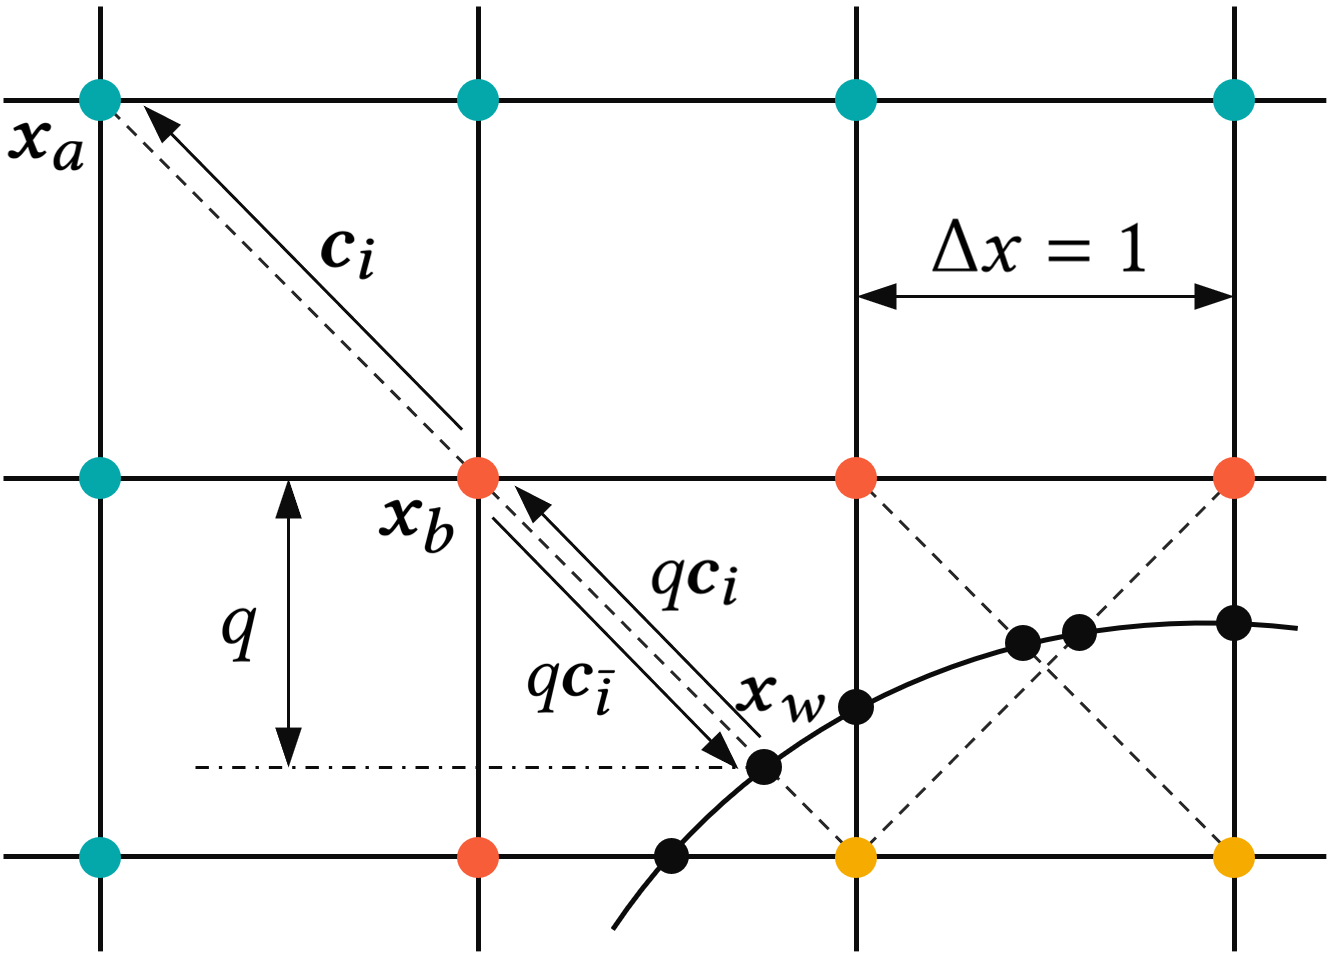
\includegraphics[width=0.6\columnwidth]{figures/boundary.png}
  \bicaption[固体附近的边界处理]{固体附近的边界处理。对于切削网格点 (图中标为橘色),它们的未知分布函数必须要通过边界处理决定。图中黄色点为固体内部点,青色点为流体点。对于$\bm{x}_b$点,$q$表达该点沿$\bm{c}_i$方向到边界的归一化距离,其中$\bm{c}_{\bar{i}}$为$\bm{c}_i$的反方向。}{Boundary treatment near solid object. For ``cut-cell'' boundary nodes marked in orange, their unknown distribution functions must be determined through boundary schemes instead of the regular streaming. Yellow nodes mark nodes inside the solid while cyan nodes are fluids nodes. Our boundary treatment for a node $\bm{x}_b$ uses the normalized distance $q$ to the boundary surface along a link direction of $\bm{c}_i$ with its inverse direction denoted as $\bm{c}_{\bar{i}}$.}
  \label{img:boundary}
\end{figure}

\begin{figure}[htb]
	\centering
	  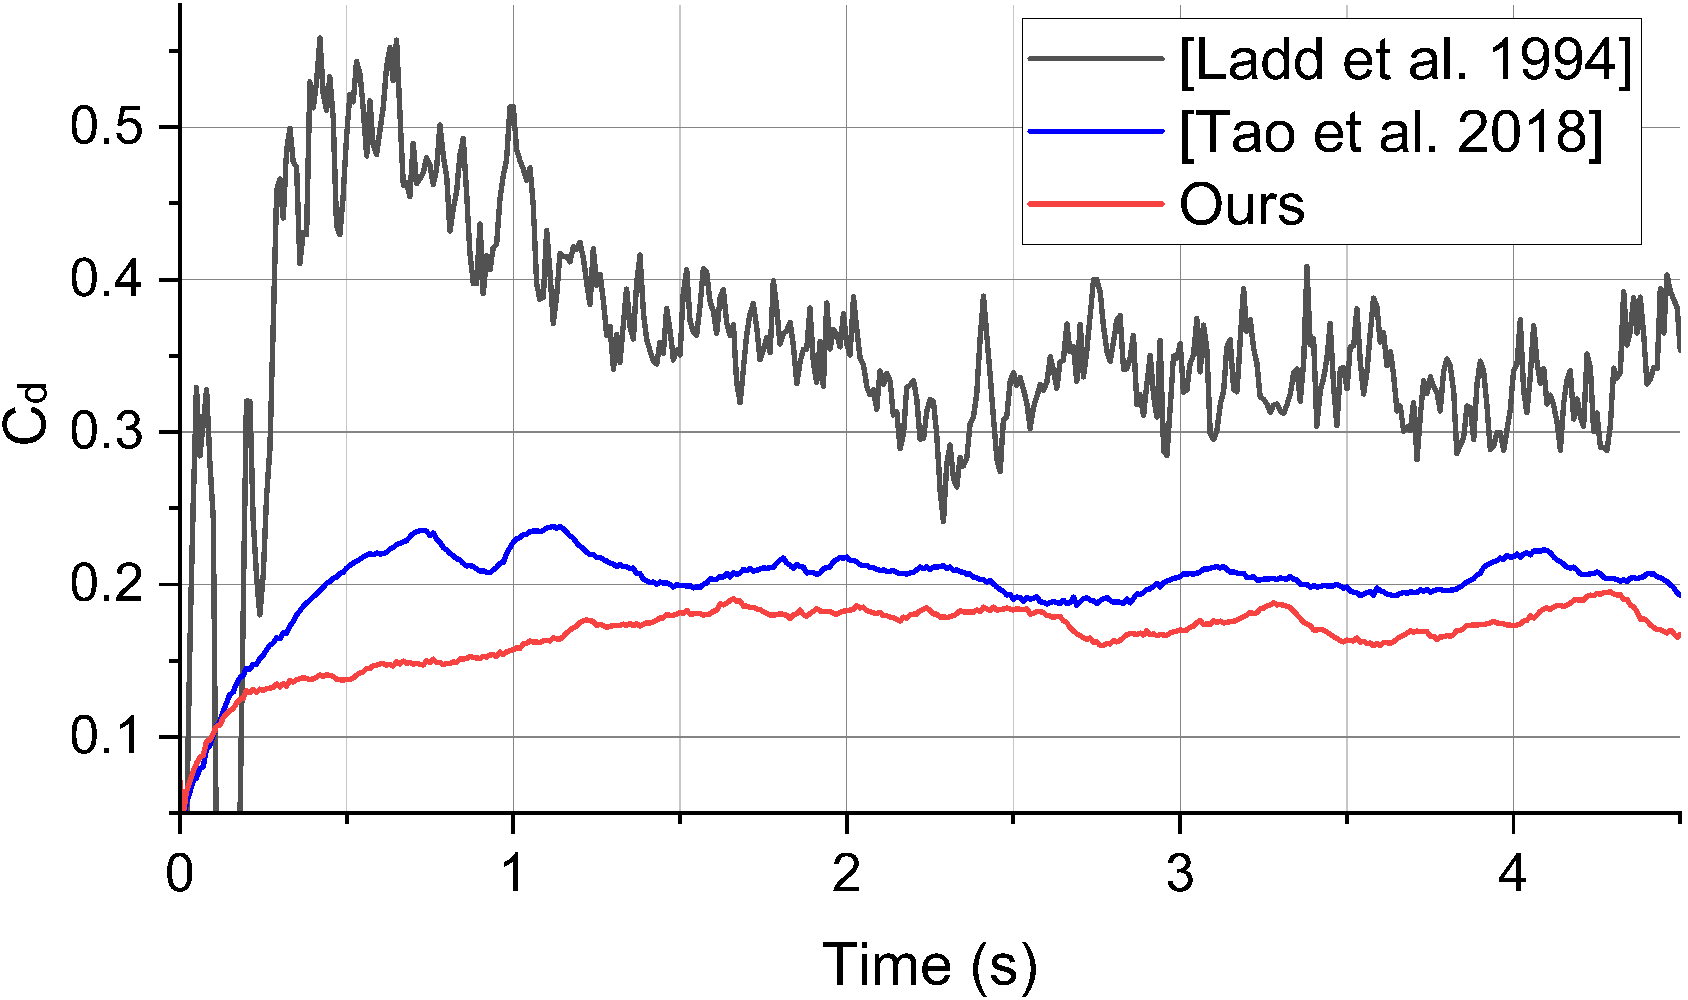
\includegraphics[width=0.7\columnwidth]{figures/bnd_comp.png}
	\bicaption[边界处理的比较]{边界处理的比较。对于$Re=400,000$风吹过球的场景,我们画出了使用不同边界处理进行仿真得到的球的阻力系数。仿真中的碰撞模型均为使用了熵优化的累积量碰撞模型。该场景在实际实验中得到的球的阻力系数$C_\text{d}\!=\!0.1$。虽然简单反弹边界依然在许多LBM中得到应用,但是其结果误差及波动均过大,无法得到可置信的结果。}{Comparing boundary treatments. We plot the variation over time of drag coefficient of a sphere at $Re=400,000$, for different boundary treatments but with the same entropy-optimized cumulant model. The experimental value is near $C_\text{d}\!=\!0.1$ for this drag crisis case; a simple bounce-back, still used in many LBM implementations, leads to unacceptable results, producing large prediction errors and wide force fluctuations.}
	\label{img:bnd_comp}
  \end{figure}

在虚拟风洞的绝大多数情况中,目的都是对某个物体进行气动的性能测试。所以在虚拟风洞的应用中,边界处理的重要性是不言而喻的。边界处理的示意图见图~\ref{img:boundary}。其中橘色点为需要进行边界处理的流体点,黄色点为固体内部点。
我们在第~\ref{sec:boundary_treatment} 节中已经讨论了简单反弹边界和插值反弹边界的形式。其中简单反弹边界虽然构造形式非常简单,但是在边界形状复杂时,一般只有一阶精度。从而在计算固体受力时,误差及波动是非常剧烈的 (见图~\ref{img:bnd_comp} 中展示的风在高雷诺数下吹过球时,球的阻力系数$C_\text{d}$变化)。
插值反弹边界~\cite{Bouzidi-2001} 与其之后的变体~\cite{Yu-2003, Ginzburg-2003, Chun-2007} 则可以使边界求解的精度达到二阶或更高。然而,这些边界处理方法均需要相邻点的参与,使得计算不再完全局部。由于GPU并行计算中,不连续数据访问对并行效率有很大影响,这样的边界处理在GPU计算上的效率有所降低。此外,当边界点周围均为边界时,找不到相邻点会使这样的边界处理方法失效。
而最近,Tao等~(\citeyear{Tao-2018-b}) 通过在边界上构造额外的分布函数,提出了一个单点的插值反弹边界方法,克服了这一问题。
具体地,如图~\ref{img:bnd_comp} 中所描绘的,我们用$\bm{x}_{b}$表达固体边界附近需要边界处理的点,$\bm{c}_{i}$为指向$\bm{x}_{a}$的方向,$\bm{c}_{\bar{i}}$为相反的方向并与固体边界相交于$\bm{x}_{w}$。跟随之前的插值反弹边界方法中的假设,我们认为这之中存在线性关系:
\begin{equation}
f_i(\bm{x}_b, t\!+\!1) = \frac{1}{1+q}f_{i}(\bm{x}_w, t\!+\!1)+ \frac{q}{1+q}f_{i}(\bm{x}_a, t\!+\!1) \;,
\end{equation}
其中$q=\|\bm{x}_b - \bm{x}_w\|/\|\bm{c}_i\|$是边界点到边界的归一化距离。
因为分布函数$f_{i}(\bm{x}_a, t+1)$可以从$\bm{x}_b$的前一时刻迁移过来,所以这里的线性插值实际上只涉及一个点的数据。
而边界上的未知分布函数$f_{i}(\bm{x}_w, t\!+\!1)$可以由平衡态$f_{i}^\text{eq}(\bm{u}_w(t), \rho_b(t))$与b点的非平衡态$f_{i}^\text{neq}(\bm{x}_b, t)$相加得到,其中$\bm{u}_w(t)$为边界点的速度。$f_{i}^\text{neq}(\bm{x}_b, t)$可以表达为
\begin{equation}
f_{i}^\text{neq}(\bm{x}_b, t) = f_{i}(\bm{x}_b, t) - f_{i}^\text{eq}(\bm{u}_b, t).
\end{equation}
然而由于这样的构造使用了低阶的泰勒展开近似,在高雷诺数仿真中精度并不足够。为了进一步提升精度,我们提出一种新的构造平衡态和非平衡态的方法。
首先,我们可以利用非平衡态的阶数比平衡态高一阶的性质~\cite{Chun-2007},意味着我们可以对$\bm{x}_b$点的非平衡态进行简单反弹,而并不会影响整体解的精度。用公式表达为
\begin{equation}
\label{eq:neq_bb}
f^\text{neq}_{i}(\bm{x}_b, t\!+\!1) = f^\text{neq}_{\bar{i}}(\bm{x}_b, t).
\end{equation}
对于平衡态部分,我们可以采用与~\cite{Tao-2018-b} 同样的二阶精度单点插值方法
\begin{align}
f^\text{eq}_i(\bm{x}_b, t\!+\!1) &= \frac{1}{1+q}f^\text{eq}_{i}(\bm{x}_w, t\!+\!1) + \frac{q}{1+q}f^\text{eq}_{i}(\bm{x}_a, t\!+\!1).
\end{align}
虽然$f^\text{eq}_{i}(\bm{x}_w, t\!+\!1)$可以由$f_{i}^\text{eq}(\bm{u}_w(t), \rho_b(t))$近似,但我们仍然需要确定如何求得$f^\text{eq}_{i}(\bm{x}_a, t\!+\!1)$。
由于我们无法获得$t+1$时刻的宏观量,一种方法是通过宏观量$\bm{u}(\bm{x}_a, t)$与$\rho(\bm{x}_a, t)$来重建平衡态。这样的做法相当于将平衡态公式对$t$进行泰勒展开后,进行了0阶逼近。这样的逼近势必在高雷诺数仿真中对边界层附近有负面的影响。
所以,我们利用$f^\text{eq}_{i}(\bm{x}_a, t\!+\!1) \approx f_{i}(\bm{x}_a, t\!+\!1)$来进行逼近,以不进行任何截断。并且$f_{i}(\bm{x}_a, t\!+\!1)$可以直接从$\bm{x}_b$迁移获得。所以我们得到
\begin{equation}
\label{eq:eq_a}
f^\text{eq}_{i}(\bm{x}_a, t\!+\!1) \approx f^{*}_{i}(\bm{x}_b, t).
\end{equation}
结合公式~\ref{eq:neq_bb} 与公式~\ref{eq:eq_a},未知分布函数$f_i(\bm{x}_b, t\!+\!1)$可以被写为
\begin{align}
f_i(\bm{x}_b, t\!+\!1) &= f^\text{eq}_i(\bm{x}_b, t\!+\!1) + f^\text{neq}_{i}(\bm{x}_b, t\!+\!1) \\
&= \frac{1}{1\!+\!q}f_{i}^\text{eq}(\bm{u}_w(t), \rho_b(t)) + \frac{q}{1\!+\!q}f^{*}_{i}(\bm{x}_b, t) + f^\text{neq}_{\bar{\imath}}(\bm{x}_b, t).\nonumber
\end{align}

\paragraph{动态耦合}
虚拟风洞中也需要一部分动态的单向耦合,如汽车仿真时轮胎的旋转。
之前的LBM通常结合格点重填与反弹边界条件~\cite{Tao-2016},或使用浸没边界法~\cite{Li-2016, Li-2020}进行动态耦合。
但格点重填结合反弹边界条件的方法在高雷诺数仿真中会在边界周围产生不正常的速度。而浸没边界法虽然更容易实现,但因为只有一阶精度,则达到同样精度需要更高的分辨率进行仿真,从而消耗更多的资源。
为了保证在薄边界层上保证更高的精度,在动态耦合时,我们依然应用上述的静态边界处理方法,不同点是现在各个切削速度方向的$\bm{u}_w$都需要求解。为了避免格点重填,我们依然使用浸没的模式来处理边界,即所有的格点我们都认为是流体点,没有固体点。当然我们注意到,要在每个时间步都进行求交并求解边界的速度,通常需要进行层级搜索~\cite{Karras-2012},而当分辨率非常高时,在GPU上进行这样的操作非常耗时。
于是我们提出了相应的GPU实现,以减轻求交与动态耦合的计算开销。这些算法我们在第~\ref{chap:sig23_alg_optimal} 节中介绍。

\paragraph{计算域边界处理}
在固体边界之外,还有一些边界也需要进行处理,其中一类就是计算域边界。计算域的边界同样对仿真得到的物理量有很大影响。我们在实现时使用了滑移边界条件 (slipping boundary conditions) 来处理入口与出口之外的计算域边界。虽然有多种方法可以实现滑移边界~\cite{Kruger-2016},但这些方法的精度不足以在强湍流中准确求解计算域边界处的流体,并会对物体附近的流体产生影响。于是我们需要扩大计算域来减轻其影响,但这样会额外增加仿真的时间和存储成本。
为了弥补这一问题,我们在计算域边界首先采用$\bm{u}_w \!=\! \bm{u}_n$的边界条件,其中$\bm{u}_n$是沿着计算域边界法向方向,距边界最近的流体点的速度。
然后使用这一边界速度,我们将计算域边界视为动态边界并使用上述方法进行处理。同样的处理也可以应用在计算域的入口或出口上。在已知速度或压力后,未知的分布函数可用同样的边界处理方法获得。我们通过这样的处理,避免计算域边界对计算域内部产生过大的影响。

\paragraph{地面处理}
由于虚拟风洞中的实验经常要与现实风洞实验相对应,很多时候模型会被放置在地面上。此时由于地面与模型距离非常接近,地面的边界处理对精度有着非常大的影响。所以在模型被放置在地面时,我们不能认为地面是普通的计算域边界,而要进行特殊处理。我们这里的特殊处理方法使用了壁面函数~\cite{Malaspinas-2014},即通过地面上方的格点与壁面函数,推导出地面速度$\bm{u}_g$。而地面的密度可以认为与地面上方的点一致 (即诺伊曼边界条件$\nabla \rho \cdot \bm{n} \!=\! 0$)。具体的宏观量推导过程由于篇幅限制,无法按步骤详细列出,请读者参见~\cite{Malaspinas-2014}。
在获得地面的宏观量之后,我们重建未知的分布函数$\smash{f_i \!=\! f_i^{eq} + f_i^{neq}}$,其中
\begin{align} 
    f_i^{eq} &\approx w_i \rho_g+\biggl(1+\frac{\bm{c}_i \cdot \bm{u}_g}{c_s^2}+\frac{\left(\bm{c}_i \cdot \bm{u}_g\right)^2}{2 c_s^4}-\frac{\bm{u}_g \cdot \bm{u}_g}{2 c_s^2}\biggr), \\
    f_i^{neq} &\approx -\frac{\tau \rho_g \omega_i}{2 c_s^2} \langle \bm{Q},  \nabla \bm{u}_g + \nabla \bm{u}_g ^ T \rangle,\\[-6mm]\nonumber
\end{align}
这里面$\smash{Q_{\alpha\beta} = c_{i\alpha} c_{i\beta} - c_s^2\delta_{\alpha\beta}}$ ($\delta_{\alpha\beta}$是克罗内克 (Kronecker) $\delta$函数)。
使用这样的壁面函数处理地面,在高雷诺数流体仿真中,依然不足以获得足够高精度的解。原因是地面可能与模型本身形成一条窄缝 (想象汽车在地面上时,底盘与地面之中的间隙),在这种情况下流体的运动情况很难被现有的LBM准确捕捉。我们注意到类似情况的边界处理仍然是热门的研究课题,所以在这一方向若有后续工作可以对地面处理部分进行改进。

\paragraph{固体受力计算}
对于上述的边界处理,我们依然可以用动量交换法计算固体受力~\cite{Ladd-1994, Mei-2002},即对于边界点$\bm{x}$有
\begin{equation}
    \Delta \bm{p}(\bm{x})= \sum_{j\in L(\bm{x})} \bm{c}_{j'}\,(f_{j}(\bm{x}) + f^*_{j'}(\bm{x})),\vspace*{-1.5mm}
\end{equation}
其中$L(\bm{x})$为$\bm{x}$点向外的速度方向 (由固体向流体方向),$f_{j}(\bm{x})$为通过边界处理方法得到的分布函数。则固体受到的合力为所有边界点上受力的和
\begin{equation}
    \bm{F} = \sum_{\bm{x}} \Delta \bm{p}(\bm{x}).\vspace*{-1mm}
\end{equation}
注意因为我们使用了浸没的思想,所以所有的切削网格点都应被视为边界点。

\subsection{多分辨率仿真}
\label{sec:multi-res}
如果我们在单分辨率网格上应用上述的算法,对于图形学领域的应用应该足够。因为一般图形学中的物体模型较为简单,且我们只需捕捉视觉现象。但应用于工程领域,虚拟风洞需要被应用至非常大的场景 (一般对于4m左右长度的汽车模型需要40m$\times$20m$\times$20m的计算域),且几何模型的精度需要有3mm或更高的解析度,以捕捉到足够小的流体特征。这些特征也许对湍流本身的视觉效果来说没有明显改变,但是它们对物理量的大小有关键的影响。使用单分辨率网格进行这样高分辨率的仿真无论从仿真时间或内存和显存的占用考虑,都是不切实际的。所以显然多分辨率网格在工业领域流体仿真应用中是不可或缺的~\cite{Hou-2019,Aultman-2022,Romani-2022}。

然而,我们已经讨论过,许多传统的基于有限体积法的N-S求解器均需要非结构化网格。对于工业精度的几何模型,构建这样的网格是十分耗时的。虽然针对非结构化网格,有自动化的网格构建方法,但是由于模型的高复杂性,网格中产生空洞或尖角的情况依然无法避免,这些会导致FVM的求解最后无法收敛。而对模型的检查、修复需要专业工程师的人工努力,这对实际工业设计中的工作效率有很大影响。

在LBM的文献中,多分辨率网格方法一般都基于八叉树的数据结构~\cite{EitelAmor-2013,Hasert-2014},但是要在GPU上完成高效且可扩展的实现是十分复杂的~\cite{Schornbaum-2016, Schornbaum-2018}。而我们提出了新的全自动网格构建算法,以支持十分复杂的几何模型与更简单、高效的GPU实现。下面我们描述该算法的具体过程。

\paragraph{多分辨率网格构建}
自动的网格细化一般都需要基于一定的标准来指导对哪一部分进行细化。这其中最常被考虑的应该是来流方向及网格到边界的距离~\cite{Sandoval-2012,Li-2019}。
于是我们也主要围绕这两个因素,设计我们的自动网格构建方法。
对于一个模型,我们首先将该模型的轴对齐包围盒 (axis-aligned bounding box, AABB) 的每个维度延长一定的距离$d^*$,这个距离表示贴体网格的厚度。至此我们得到了一个比模型稍大的方形区域$\Omega_n$ (见图~\ref{img:grid_construction} 中的红色方框区域)。为了方便网格间的数据过渡,从粗到细,每层格子间的网格大小均是上一层的2分之1。同时格子间要有部分的重叠以减小网格数据过渡的误差。
下面我们将整个计算域标记为$\Omega$,并将纯流体区域标记为$\Omega_f \!=\! \Omega \setminus \Omega_n$。在$\Omega_f$中,我们主要考虑来流方向。
即$\Omega_f$中的所有网格均会沿来流方向延伸,以用更细的网格覆盖物体后的尾流部分 (见图~\ref{img:grid_construction} 中从蓝色到黄色的网格)。
而在$\Omega_n$中,我们对每一个点计算一个到模型的距离,构成一个无符号距离场 (我们会在下面讨论为什么不使用有符号距离场),之后保留所有距离小于$d^*$的点 (见图~\ref{img:grid_construction} 中的橘色网格)。在计算距离场时,我们使用了Imre等~(\citeyear{Imre-2017}) 提出的高效GPU距离场计算方法。通过这样我们得到的多分辨率网格并不需要树形结构进行组织,同时也可以使各层网格间顺利地进行数据过渡,而避免Li等~(\citeyear{Li-2019}) 所提出的连续尺度方法中大量的内存及显存消耗。

\paragraph{针对动态物体构建网格}
为了应用于虚拟风洞测试,我们必须考虑一定的动态物体。由于风洞中需要双向耦合的频率远低于单向耦合,所以这里我们只考虑单向耦合。依然从该物体的AABB出发,我们将该模型所有可能经过的位置都设为最细的网格区,以满足边界附近的精度。这样的构建对如轮胎旋转等物体绕轴旋转的场景十分适合,因为物体的运动几乎不会扩大网格覆盖的范围。但是对于更复杂的运动,如飞机的起落架从机腹中落下这样的场景,虽然可以使用同样的方法构建网格,但会浪费大量的细网格,从而造成显存浪费。我们认为这一部分可以在未来工作中有所改进。

\begin{figure}[htb]
	\centering
	  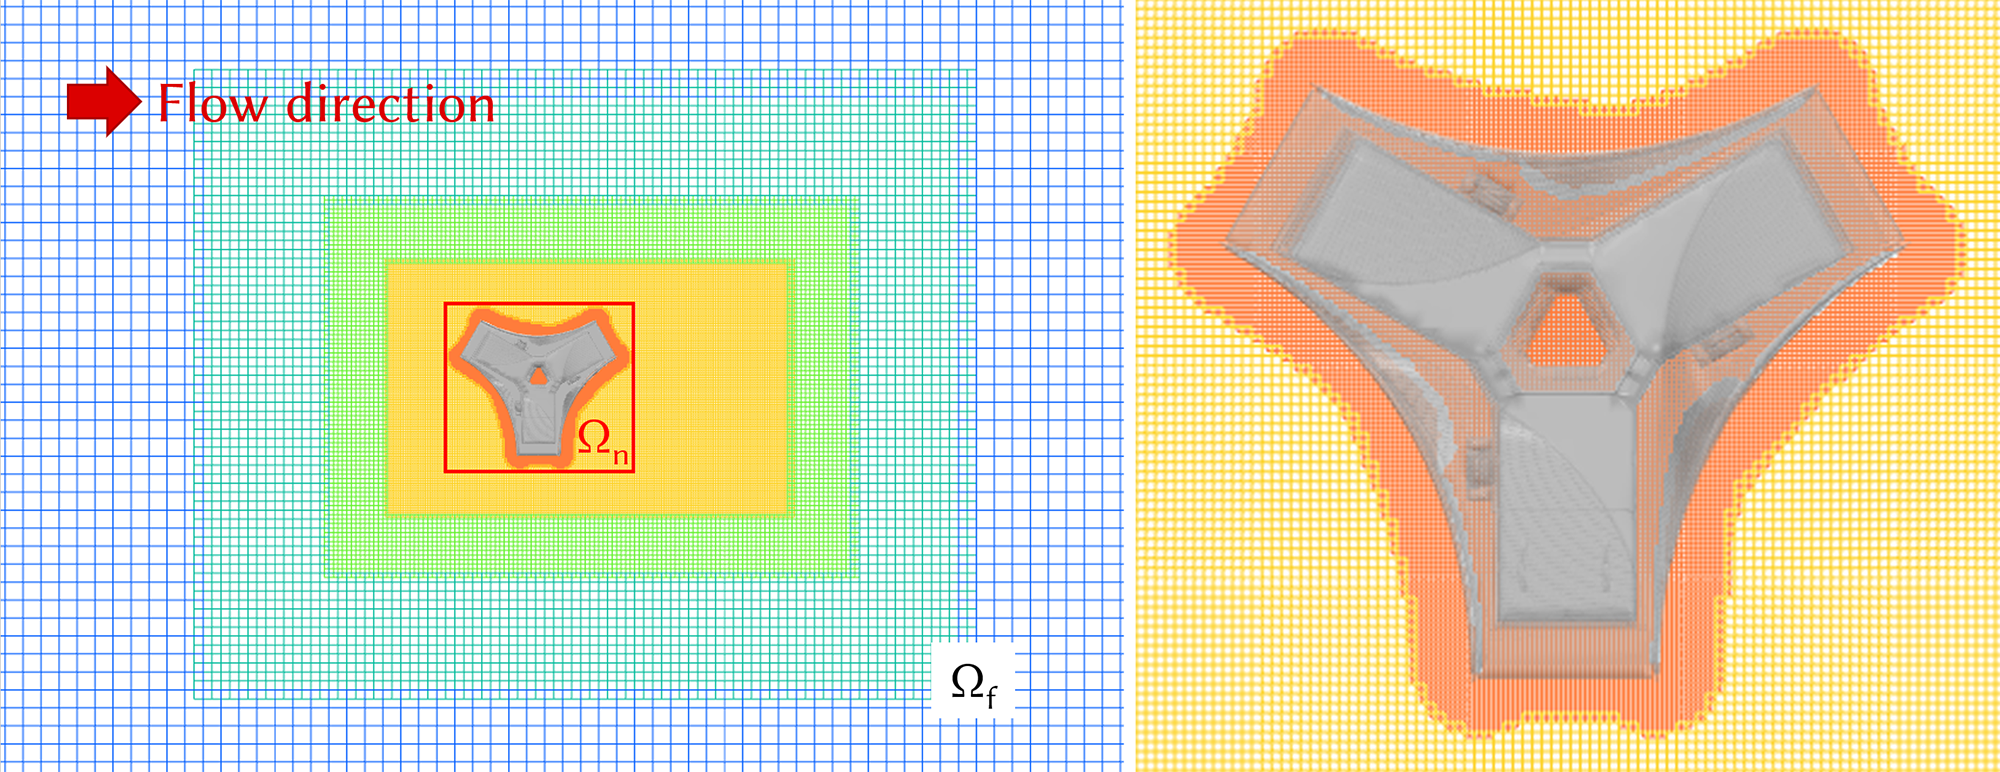
\includegraphics[width=0.9\columnwidth]{figures/grid_construction.png}
	\bicaption[多分辨率网格的构建]{多分辨率网格的构建。为了尽可能在节约内存与显存使用的同时,依旧维持足够的仿真精度,我们依据来流方向对所有网格进行自动构建 (最后一层网格除外,见左图)。即除最后一层网格外,每一层网格均有一定的方向性扩展。这个扩展是为了更准确的捕捉建筑物模型后的尾流。最后一层网格依据到边界的距离进行构建。最后我们通过传播找到所有的有效流体点,以保证场景中每一个连通部分都可以参与流体计算 (前提是这些连接部分至少大于最细网格的大小,见右图)。}{Multiresolution grid construction. To keep memory size low when computing accurate predictions of physical quantities, multiresolution grids are automatically constructed, with a refinement guided by the incoming flow direction for all but the last grid level (left) --- explaining the offset of the different levels of grid compared to this architectural building so as to capture its wake accurately --- then by the distance to the object. All active fluid nodes are finally found by flooding to ensure that the flow goes through all the mesh openings larger than the finest grid resolution (right).}
	\label{img:grid_construction}
  \end{figure}

\paragraph{针对复杂物体构建网格}
如果我们认为物体模型至少是闭合的,那么我们通过有符号距离场 (signed distance field) 已经可以有效地分辨格点位于物体的内外。但是在实际应用中,很多模型并不具有这样的良好特质。如汽车的栅格实际上可以视作汽车内部的空气入口,建筑模型也有很多很小的开口足以使空气流入。
在这种情况下,我们无法实际判别物体内外。所以我们在最细的网格上使用一个传播算法,来标记所有有效的网格点。具体地说,我们从一个已知的流体点出发,如$\Omega_n$中的网格原点,沿各个速度方向检查该点与其邻居是否相连。相连的标准为它们之间的速度方向是否与物体边界相交,若相交则认为不连通。该过程的一个二维示例见图~\ref{img:propagation}。
我们将所有连通的点标记为有效流体点后,继续重复这一过程,进行广度优先搜索,以找到所有的有效流体点。
这样做的好处主要有两个。第一个为我们可以剔除掉所有的固体点,因为固体点对仿真没有实际影响。这样我们可以进一步节省显存占用。第二个为我们可以同时将边界处理时所需要的归一化距离$q$一并求出,留至之后边界处理时使用。

\paragraph{网格间数据过渡}
接下来我们必须考虑数据如何在不同网格大小的网格间传递、过渡。这一方面我们使用了~\cite{Lagrava-2012} 中提出的方法。该过程可简要概括如下。对于两个网格之间的数据交互,永远存在一个较粗的网格和较细的网格 (两个网格的网格大小是2倍关系),并且这两个网格中会有一定的重叠区域以方便过渡 (这些在我们的网格构建方法中已经通过约束保证)。那么粗、细网格会交替执行仿真。由于网格大小的2倍关系,为了保证同样的黏度,它们的时间步长也是2倍关系,即粗网格仿真一个时间步长,细网格需仿真两个时间步长。在这两个网格中,最外层的格点均可视为需要进行网格过渡的格点 (我们接下来称为待求点),因为它们的分布函数信息无法靠自己获得,只能从另一网格获得。而因为重叠区域的存在,细网格的待求点在粗网格中是正常格点。同理,粗网格的待求点在细网格中也是正常格点。所以,在两个网格交替前进时间步长的过程中,待求点的信息都可以从另一个网格插值得到。而这个插值需要分为平衡态与非平衡态。因为平衡态部分只取决于宏观量,而宏观量在不同网格中是不变的。但非平衡态部分与应力张量有关,在不同网格间有一定的比例关系,所以在不同网格间插值时需要进行缩放。关于整体数据过渡的细节可参考~\cite{Lagrava-2012}。
这一过程其实对于每一对 (粗、细) 网格都是相同的,所以可以从粗到细以递归的方式完成。
% Fig.~\ref{img:vis_building} for instance shows an instantaneous macroscopic velocity field cross-section from the simulation of the same architecture model from Fig.~\ref{img:grid_construction} using this interpolation approach.

\begin{figure}[htb]
    \centering
      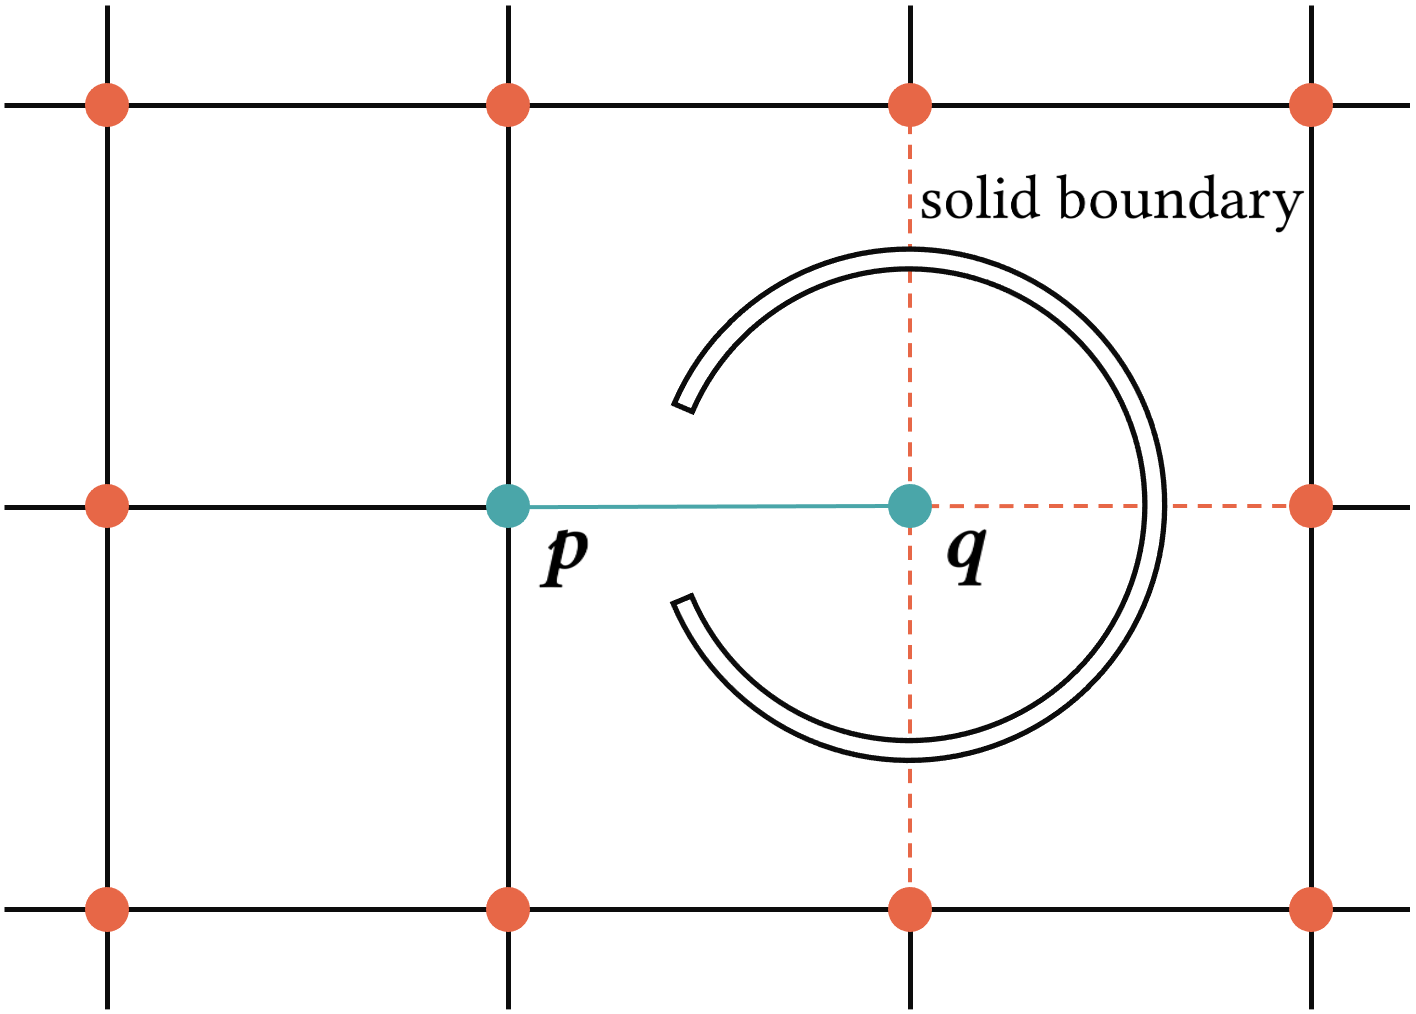
\includegraphics[width=0.7\columnwidth]{figures/propagation.png}
    \bicaption[通过传播找到有效的流体点]{通过传播找到有效的流体点。为了找到并标记所有有效的流体点,我们从一个已知的流体点出发 (如图中的$\bm{p}$点),然后我们找到该点所有的邻接点,检测它们之间的连接有没有与固体边界相交。如果两点间的连接没有与边界相交 (如$\bm{p}\bm{q}$),则点$\bm{q}$被标记为新的有效流体点。这个过程以广度优先顺序重复,直到找到所有有效的流体点,使所有的连通部分相互连接}{Propagation of valid fluid nodes. To find and tag all valid fluid nodes, we start from an already known fluid node, e.g., node $\bm{p}$ in 2D, then we check its immediate neighbors to see whether a link intersects a boundary. If no intersection is detected (e.g., link $\bm{p}\bm{q}$), the untagged node $\bm{q}$ is tagged as a new valid fluid node. This process repeats in a bread-first search order, enabling internal regions to be connected to the external fluid region.}
    \label{img:propagation}
\end{figure}

\section{算法优化}
\label{chap:sig23_alg_optimal}
我们接下来讨论一些我们在实现过程中发现的,对计算效率有重要影响的方面,及我们的优化方法。
% An overview of our simulation process is summarized in Alg.~\ref{alg:simulation}.

\paragraph{高效链路-几何求交}
在边界处理中,每一步我们都需要得到边界点上各链路到几何模型的距离。对于静止模型,我们可以只在前处理中做一次求交,但是对动态物体,由于其形状在不停改变,我们需要在每个时间步都进行一次求交。由于求交的复杂性,这一步在时间上的消耗甚至大于仿真本身的消耗。
为了解决这一问题,我们采用与浸没边界法~\cite{Chen-2021}中的扩散 (spreading) 类似的想法,以物体模型的元素为出发点,寻找周围的流体点,而不是以流体点为并行单元进行并行。
对于边界上的每个元素 (在三维中通常为三角形),我们找到所有该元素覆盖的网格。这一步只需不遗漏网格即可,所以使用该元素的AABB也是可以的。这一过程的一个二维示意图可见图~\ref{img:intersection},在二维中模型元素是线段而不是三维中的三角形。
对于每个覆盖的网格,格点上的所有链路都会与该模型元素进行求交测试。如果有链路相交,则我们在这个格点上记录归一化距离$q$,这个距离会在边界处理中被使用。
这样做的优势是,每个模型元素所找到的流体点的数量都是相对较少的,这在GPU上有着数据连续和负载均衡的优势。为了测试效率,我们使用一个4.5 m长的、元素数量在1千万的模型,在一个网格大小为4 mm的计算网格中求交。结果显示使用上述的求交方法,相比传统的树状结构加速的方法,效率的提升在大约十倍。这可以有效地提升整体仿真的计算效率,尤其是场景中有动态物体时。

\begin{figure}[htb]
  \centering
    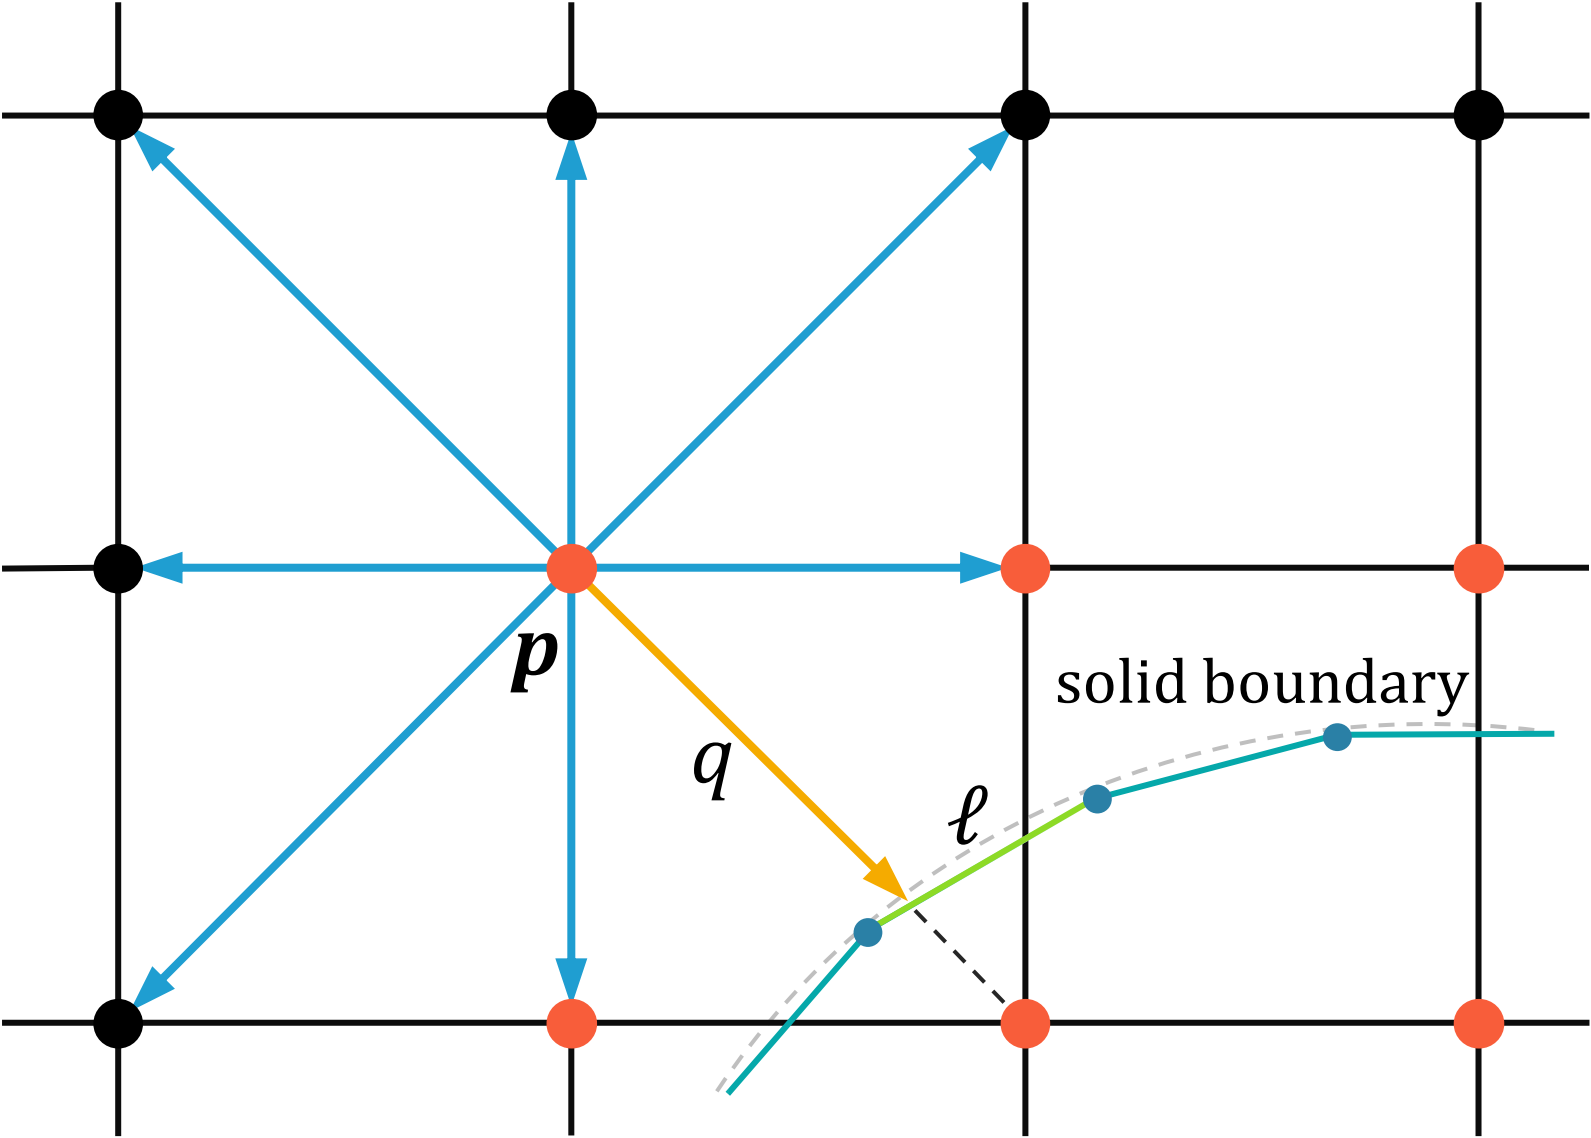
\includegraphics[width=0.7\columnwidth]{figures/intersection.png}
  \bicaption[高效链路-几何求交]{高效链路-几何求交。我们不使用传统方法,即将模型的元素放入一个树形结构中进行查找。我们使用以模型元素作为并行单元,来查找附近和其相交的链路。这里在二维中,模型元素是线段,而三维中一般是三角形。对于一个模型元素,我们可以很快地找到其所覆盖的网格,并于可能相交的链路依次求交。}{Efficient link-boundary intersection. Instead of building a tree-based data structure, we parallelize our link-mesh intersection over all boundary elements --- here boundary edges $\ell$ in 2D. For a given boundary edge, we efficiently locate the cells that the edge straddles, and perform intersection for every link of the nodes that belong to the covered cells.}
  \label{img:intersection}
\end{figure}

\paragraph{数据布局}
在LBM中,分布函数的迁移是必须要访问邻接点的。而GPU中数据的访问顺序又直接影响显存的数据吞吐量,进而影响计算效率。所以设计一定的数据布局以适应LBM的访问对LBM的效率也有很大影响 (尤其是在多分辨率网格中)。
首先整体上,我们依然使用~\cite{Chen-2021} 中的数组结构体结构。一个需要注意的点是,我们构建出的网格中,有效流体点并不一定连续,所以我们需要一个紧凑且GPU友好的数据结构来存储有效流体点的索引。然而在我们的测试中,完美空间哈希 (perfect spatial hashing)~\cite{Lefebvre-2006} 或用于稀疏矩阵的紧凑存储结构~\cite{Greathouse-2014} 表现均不够好。在测试中两者均会增加显存读取频率并使数据访问更不连续,造成计算效率下降。使用针对不规则数据的z-排序 (z-ordering) 结构~\cite{Chen-2021} 也并没有获得预期的性能提升。
所以,为了实现简单,我们生成了一个简单的索引映射 (index map),即以x-y-z顺序,直接在一个线性数组中记录所有流体点的显存索引。这样的数据布局与~\cite{Chen-2021} 中的基于块的存储方法的性能接近,但实现会简单很快。我们认为多分辨率LBM网格的数据布局也是未来可以改进的方向之一。

\section{与现有方法的对比}
\begin{figure}[htb]
  \centering
    \includegraphics[width=0.99\columnwidth]{figures/entropy_comp.png}
  \bicaption[不同累积量模型的对比]{不同累积量模型的对比。我们分别用~\cite{Geier-2017} (图中黑色曲线) 与我们的方法 (图中红色曲线) 对球进行风洞实验,并将$C_\text{d}$随时间的变化画在图中。我们分别在雷诺数Re=100,000 (a)、Re=400,000 (b) 与Re=800,000 (c) 时进行实验,Re=400,000 为球发生阻力危机时的雷诺数。从图中可以看出,我们的方法有着更快的收敛速度与更小的结果波动,使我们方法更适合于计算物体的平均阻力。}{Comparing drag for various cumulant models. We plot drag coefficient $C_\text{d}$ over time for a sphere in a flow using the cumulant model of~\cite{Geier-2017} (black) vs. our entropy-based cumulant model (red) for Re=100,000 (a), Re=400,000 (b) at which drag crisis happens, and Re=800,000 (c) indicating better performance of our model as evidenced by faster convergence and smaller fluctuations --- which both imply a more reliable mean drag estimation.}
  \label{img:entropy_comp}
  \end{figure}

\paragraph{与现有碰撞模型的对比}
为了验证我们的基于熵优化的碰撞模型的精度,我们对高雷诺数下物体的阻力系数$C_\text{d}$进行仿真测算,来对不同的方法进行比较。我们分别使用了我们的基于熵优化的累积量碰撞模型与现有的松弛系数只优化至3阶的累积量碰撞模型~\cite{Geier-2017} 进行仿真,仿真的场景为空气流过静止的球。我们使用这一场景进行测试的原因是球在这样的场景中会发生阻力危机 (drag crisis) 现象。该现象是指,球在雷诺数$Re=100,000$时,阻力系数约为0.47,但随着雷诺数的升高,球受到的阻力会突然且剧烈地下降,至雷诺数$Re=400,000$时,球的阻力系数会下降到约0.1~\cite{Tiwari-2020}。这样的剧烈变化对于数值流体仿真来说是非常难复现的,所以非常能体现不同仿真方法的精度与能力,而最近~\cite{Geier-2017-b} 第一个使用LBM对该现象进行了仿真。

我们在三个不同的雷诺数下进行了仿真,分别为$Re=100,000$、$400,000$和$800,000$。在这三个雷诺数下的仿真结果与实际实验值一并可见图~\ref{img:entropy_comp},实验值来自~\cite{Barati-2014}。图~\ref{img:entropy_comp} (a) 展示了,相比~\cite{Geier-2017},我们的方法可以更快地收敛并得到更贴近实验值的结果。对于更高一些的雷诺数 (阻力危机发生时),两种仿真方法都无法非常精准地预测阻力系数,如图~\ref{img:entropy_comp} (b) 中所示。但是对这个区域通过DNS进行准确仿真一般认为也是十分困难的~\cite{Tiwari-2020}。由于在这个区域边界上会生成很多小尺度的涡流,所以阻力的波动应该会减小~\cite{Deshpande-2017}。从结果中可以看到,我们的模型相对~\cite{Geier-2017} 展示出了更小的波动,这表示出我们的基于熵优化的碰撞模型在物理量上有更强的可预测性。
图~\ref{img:entropy_comp} (c) 展示了我们的新的碰撞模型在初期收敛之后,产生了周期性的波动。而原先的方法产生了一些不规则的波动,没有提供有意义的可置信区间,以评估平均阻力。

进一步讨论我们的方法,我们可以认为我们的自适应松弛系数,包括~\cite{Geier-2017} 中的三阶松弛系数优化在内,可以被认为是某种亚网格模型。这也解释了为什么我们的LBM方法在没有使用湍流模型的情况下,依然比其它基于N-S的求解器在类似分辨率下能更好地捕捉到阻力危机现象。
当然,在我们的方法中加入一个真实的湍流模型,如k-$\omega$模型~\cite{Menter-1994},也并不冲突,且这样在理论上可以更好地求解亚网格流体,但是同时求解的计算时间也会显著增加。而使用我们的基于熵优化的优化方法,并不会显著地降低效率。与 \cite{Geier-2017} 相比,我们的自适应松弛系数计算只使得碰撞过程慢了约10\%,整个过程慢了约5\%。

\begin{figure}[htb]
  \centering
    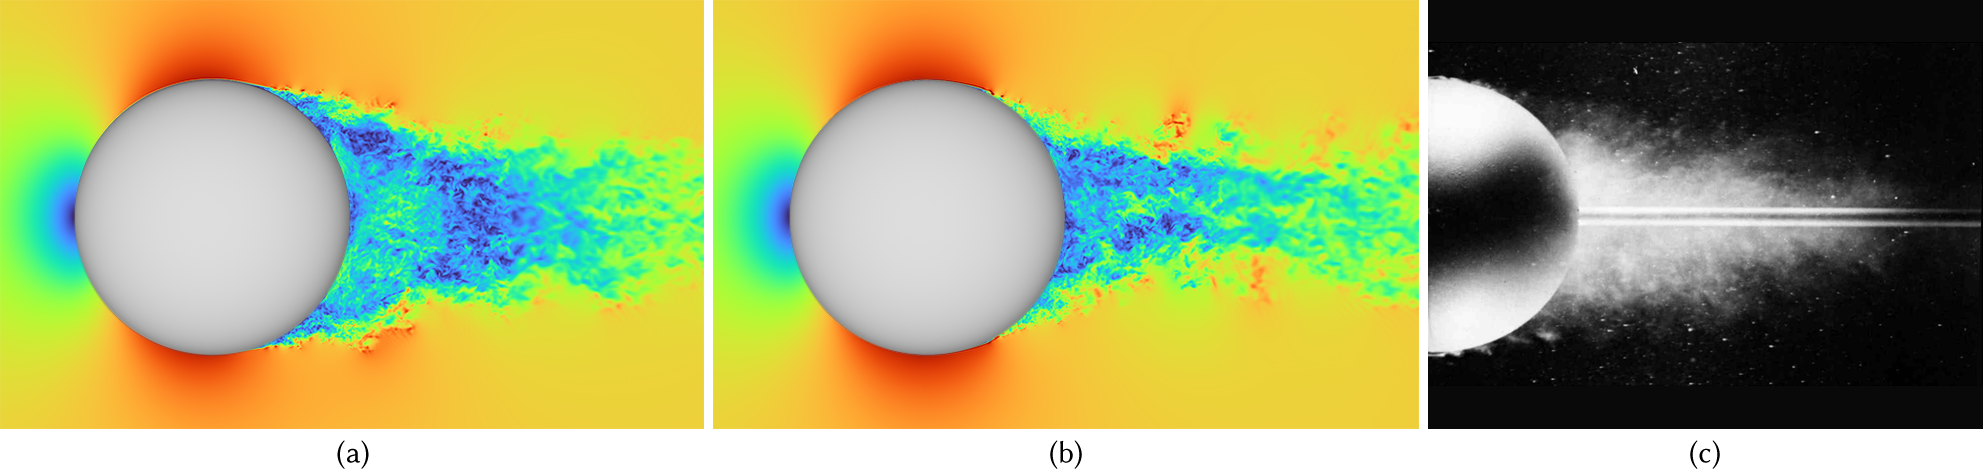
\includegraphics[width=0.99\columnwidth]{figures/wake_comp.png}
  \bicaption[球在发生阻力危机时的尾流]{球在发生阻力危机时的尾流。气流在$Re=400,000$下流过球时,由于固体边界附近的涡的尺度更小,尾流会收窄,从而阻力会下降。这一现象可见实际实验~\cite{Van-1982} (c)。与~\cite{Tao-2018-b} (a) 相比,在同样雷诺数下,我们的边界处理 (b) 捕捉到的边界的分离点更靠后,与实际实验更为接近。}{Wake of sphere in drag crisis. The flow passing through a sphere at $Re=400,000$ is known to exhibit in real-life experiment a narrower turbulent wake than at lower Reynolds numbers~\cite{Van-1982} (c) due to smaller scale vortices generated near the solid boundary, thus reducing drag significantly --- a paradox explained by the boundary-layer theory. Compared to~\cite{Tao-2018-b} (a), our improved boundary treatment scheme at the same Reynolds number (b) captures the separation point farther around the back of the sphere with a narrower wake, better matching the experimental visualization.}
  \label{img:sphere_wake_comp}
\end{figure}

\paragraph{与现有边界处理的对比}
为了验证我们的方法在边界处理上的精度提升,我们依然对雷诺数$Re=400,000$时,风流过球的阻力危机进行实验。如图~\ref{img:sphere_wake_comp} 所示,与实际实验的可视化相比 (图~\ref{img:sphere_wake_comp} (c)),我们的方法可以更好地预测固体边界附近的速度场及分离点 (图~\ref{img:sphere_wake_comp} (b))。并且,在图~\ref{img:bnd_comp} 中我们展示了不同方法得到的$C_\text{d}$与时间曲线,可见我们的方法得到的结果与真实实验最为匹配。这也说明在同样分辨率下,我们的方法与~\cite{Tao-2018-b} 相比,可以在固体边界上产生更小的涡流,使得尾流可以更加收敛,以在高雷诺数湍流仿真中获得更精准的结果。

\begin{figure}[!htbp]
\centering
  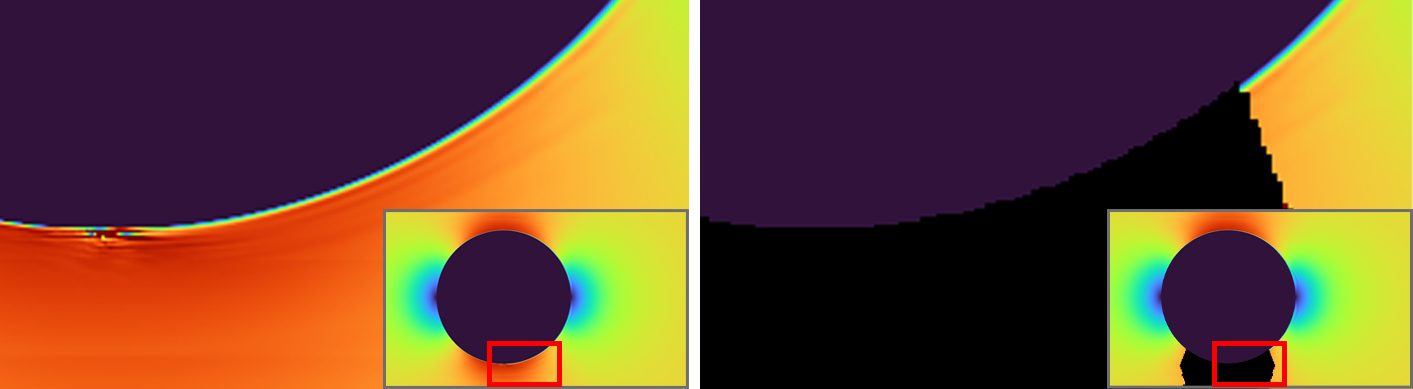
\includegraphics[width=0.99\columnwidth]{figures/wei_crash_vis.png}
\bicaption[图形学领域中最前沿的LBM方法的发散结果]{图形学领域中最前沿的LBM方法的发散结果。现有的图形学领域中的LBM方法都依赖于中心矩碰撞模型~\cite{Li-2020}。由于中心矩中的不同阶数的矩相对并不独立,且高阶松弛系数不一定准确,在使用多分辨率网格进行仿真时通常会得到发散结果,即使雷诺数并不足够高。这里展示了使用中心矩碰撞模型对$Re$=100,000时风吹过球的仿真结果。边界附近的速度求解错误 (左图) 最终导致整个求解结果发散 (右图中黑色区域)。}{Typical blowup of latest LBM solvers in CG. Existing LBM methods in CG mostly rely on central-moment collision models~\cite{Li-2020,Lyu:2021}. Due to the entangling of various orders of moments and improper high-order relaxation rates, they often blow up at low Reynolds numbers (here, $Re$=100,000) when simulating even a simple flow around the sphere with multiresolution grids, see black region (right), due to spurious velocities near the solid boundary (left).}
\label{img:wei_crash_vis}
\end{figure}

\paragraph{与图形学领域中LBM方法的对比}
虽然目前图形学领域中最前沿的LBM方法~\cite{Li-2020} 相比图形学领域中其它的流体仿真方法,已经显著地提升了精度与效率。但是对于工业领域的应用,这些方法在精度和稳定性上均有一定的差距。图~\ref{img:wei_crash_vis} 展示了一个使用图形学领域中的LBM方法进行的相对简单的气动仿真实验,即球在相对较低的雷诺数 ($Re$=100,000) 下的气动仿真。该仿真使用了与其它的球的气动仿真实验一致的多分辨率网格设置,但即使在分辨率相对较高的情况下,在仿真早期便开始出现不稳定现象,以至于数值发散而无法获得结果。

\section{方法的局限性}
我们的方法中也有一定的局限性。
首先,动态物体的精准处理在LBM中依然是一个待解决的问题,在我们的方法中,在静止场景求解时要比动态场景更加精准 (虽然这对于大部分流体求解方法也是类似的)。这一问题在第~\ref{chap:results_industry} 节的测试中有所体现。如何改进LBM的动态边界条件以获得更高的精度值得更深层的研究。
其次,在不规则网格中,我们采用的数据结构并没有足够的优化。这一问题在第~\ref{chap:sig23_alg_optimal} 中已有讨论,我们认为在这一方面也有一定的优化空间。
最后,LBM求解器与N-S求解器相比,通常需要更多的格点数与内存占用来达到相同的精度 (虽然LBM的效率要高得多)。如何减少LBM的内存消耗也是非常值得研究的方向。

\section{总结}
在本章中,我们提出了一个多分辨率的LBM流体仿真框架,以高效且准确地构建一个虚拟风洞测试系统,以评估模型的气动特性。
我们的方法基于现有CG与CFD领域中最先进的方法,在精度和效率上有所提升。这使得我们的方法可以不仅应用于视觉特效中的复杂流体仿真,也可以应用于如汽车、飞机、建筑等的设计、预览和评估,并通过快速的气动特性的反馈与分析,加速各个过程。

同时,我们的方法还弥合了CG与CFD领域中的方法差异。虽然CFD领域中不断在精度上对方法进行改进 (如更精准的碰撞模型与边界处理方法),但对求解器之外的一些重要方面,CFD领域甚少关注,如自动的多分辨率网格构建、高效的几何前处理与GPU实现等。这些在工业应用中也是十分关键的。而CG领域中,相比目前广泛使用的N-S求解器,通过使用我们的方法可以更简单、高效地完成湍流仿真与一些复杂的流体现象,这在之前的CG应用中是经常缺失的。

基于我们的工作,可以进行一些后续的工作。
首先,我们目前只处理了单向耦合,以处理虚拟风洞实验中最常见的场景。但增加对双向耦合的支持可以使我们的方法更加灵活,对实际工程与动画制作都有一定的应用价值。
此外,目前对于动态物体,我们的网格是不变的。支持动态的网格重构可以使内存使用进一步下降 (虽然可能会降低整体仿真效率)。
最后,构建一个虚拟的水下测试环境 (可以基于~\cite{Wei:2022, Wei:2023} 的工作) 以应对更复杂的场景也是一个极有意义但同时也极具挑战性的工作。
\chapter{对比与结果}
\label{sec:results}

在本章中,我们展示我们的流体仿真方法在不同领域中的应用。为了简洁,我们将第~\ref{sec:siga21} 中描述的方法称为\emph{图形方法},第~\ref{sec:sig23} 中描述的方法称为\emph{工业方法},以区分其主要面向的应用领域。

\section{面向工业应用的仿真结果与对比}
为了验证我们的虚拟风洞系统,我们从易到难的进行了三组对比实验。所有的实验都有实际风洞的测试结果,以与我们的仿真结果进行定性与定量的对比。这三组实验分别为球的阻力危机、高尔夫球的气动特性与DrivAer标准汽车测试模型的气动特性。下面我们将依次描述这三组实验。

\begin{figure}[htb]
\centering
  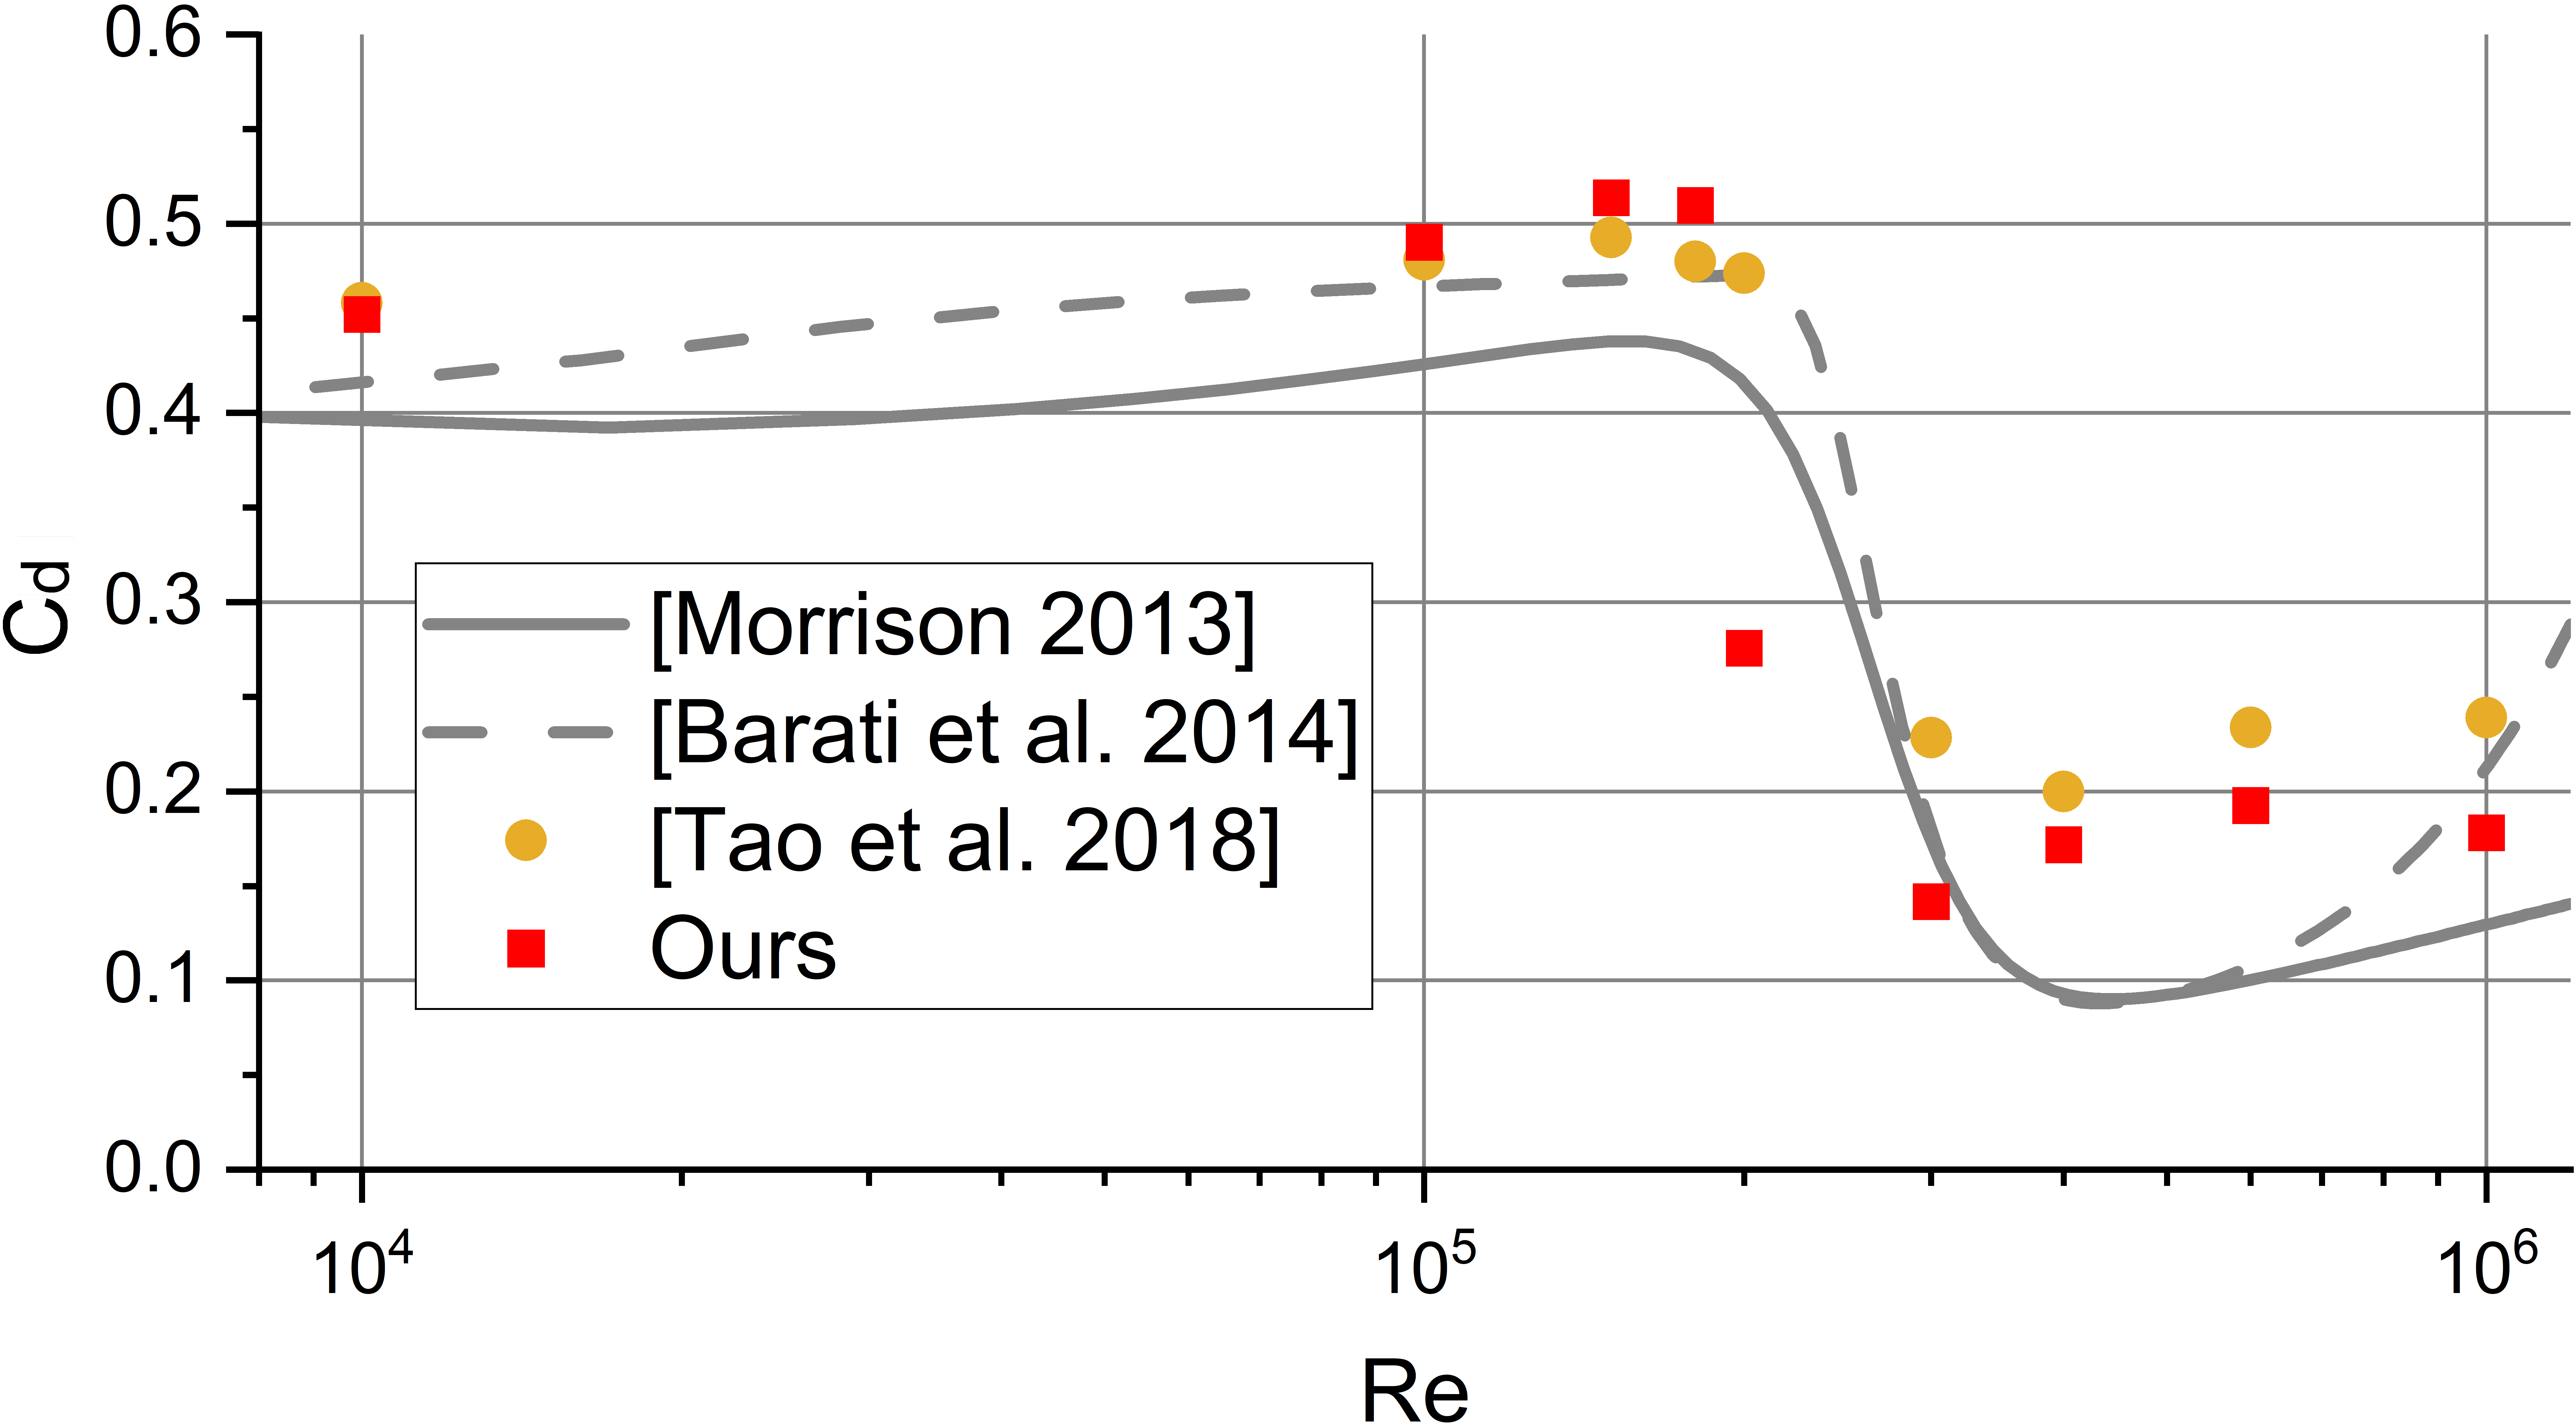
\includegraphics[width=0.8\columnwidth]{figures/sphere_cd_comp.png}
\bicaption{球的阻力与雷诺数的关系。在我们的仿真中,球在雷诺数在Re=400,000 (阻力危机) 时,\cite{Tao-2018-b} 与我们的方法都展示出了一个突然的阻力下降,之后又稍有上升,与实际实验~\cite{Morrison-2013,Barati-2014} 一致。}{Drag of a sphere vs. Reynolds number. Just like real-life experiments~\cite{Morrison-2013,Barati-2014} exhibit a sudden drop in drag for a sphere at a Reynolds number around Re=400,000 (drag crisis), both \cite{Tao-2018-b} and our kinetic solver demonstrate a similar drop at roughly the same Re, followed by a partial drag recovery.}
\label{img:drag_comp}
\end{figure}

\begin{figure}[htb]
\centering
  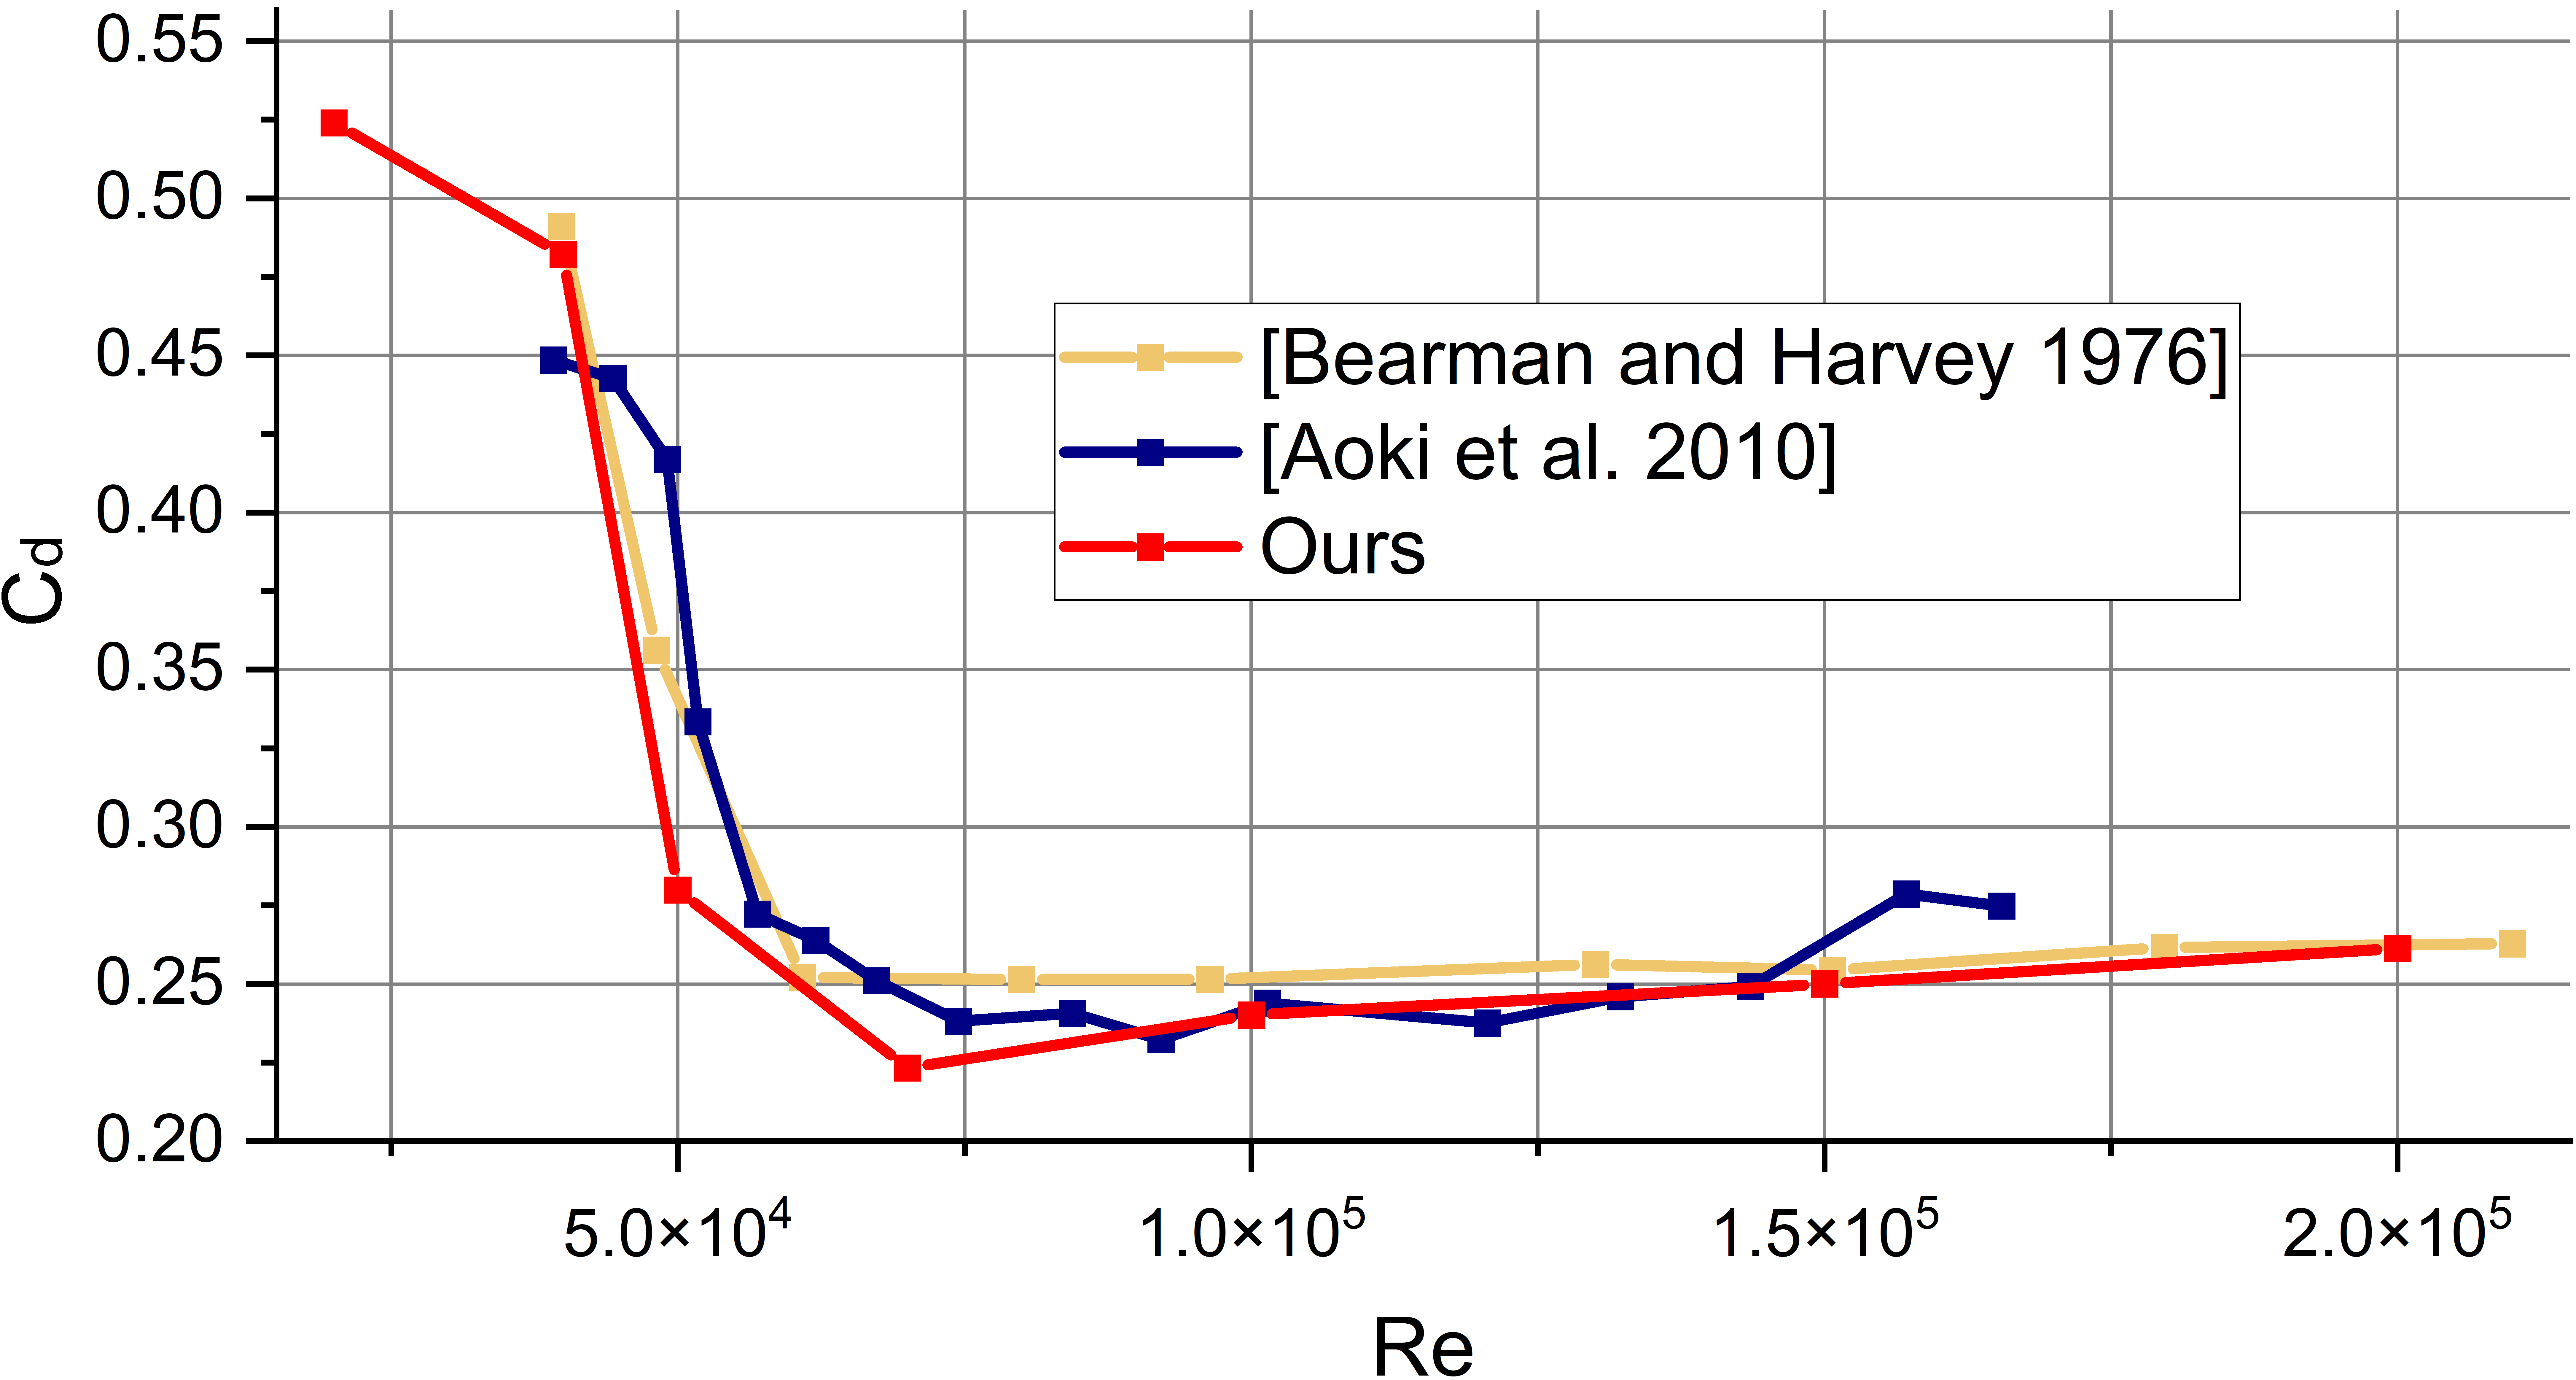
\includegraphics[width=0.99\columnwidth]{figures/golf_ball_cd.png}
\bicaption{高尔夫球的阻力与雷诺数的关系。图中绘制了高尔夫球的阻力系数与雷诺数之间的关系,与真实实验~\cite{Bearman-1976,Aoki-2010} 相比,我们的仿真给出了十分相近的结果。注意高尔夫球阻力突然下降 (阻力危机) 的位置与先前图~\ref{img:drag_comp} 所给出的光滑球相比,雷诺数要小得多。}{Drag of golf ball vs. Reynolds number.Compared to the real-world experiments reported in~\cite{Bearman-1976} and~\cite{Aoki-2010} for the drag coefficient of golf ball as a function of the Reynolds number Re, our wind tunnel simulator provides very similar evaluations. Note that the drop in drag coefficient (drag crisis)  happens far earlier than in the case of a smooth sphere, as expected --- see Fig.~\ref{img:drag_comp}.}
\label{img:golf_ball_cd}
\end{figure}

\paragraph{球的阻力危机}
阻力危机是一个很特殊的空气动力学现象,我们用风吹过球的场景对这一现象进行简单描述。可以想象,球在风中是受到了一定的阻力的,通过实验人们发现这个阻力的大小与雷诺数有关。随着雷诺数的上升,起初阻力没有大的变化。但在到达某一个特定的雷诺数后,球受到的阻力会快速且剧烈地下降。这个雷诺数我们可以称为临界雷诺数。这一现象被成为阻力危机现象。想要在数值仿真中预测这一现象是十分具有挑战性的,尤其在没有湍流模型时,因为这一现象要求求解器对边界层必须求解得足够精准。
需要说明的是,球得阻力危机发生在很高的雷诺数条件下,并且受到实际实验条件限制,精准地获取阻力系数也是十分困难的。所以在我们参考的实际实验数据中~\cite{Morrison-2013, Barati-2014},不同的实验数据也有一定的差异。而图~\ref{img:sphere_wake_comp}(c) 中的实验可视化是通过在球上添加了一个额外的环来增加有效雷诺数,从而在低雷诺数环境中进行的等效实验。
我们的虚拟风洞系统可以定性地重现阻力危机这一现象 (见图~\ref{img:drag_comp} ),即在正确的临界雷诺数,球受到的阻力产生明显且剧烈的下降。并且相比使用~\cite{Tao-2018-b} 的LBM求解器,我们的方法在临界雷诺数及之后的范围中预测的阻力系数更接近实验值。
我们注意到,我们预测出的阻力在临界区域中与实验值相比有一个小的偏移,使得在Re=200,000时我们的预测结果与实验值有一个较大的偏差。关于这一点,我们需要说明的是,即使是实际实验中,阻力系数也是在剧烈变化的。我们这里列出的实验获得的阻力系数值可以被认为是一个时间段内的平均。在这样一个流体正在发生从临界雷诺数前到临界雷诺数后转变的过程中,数值仿真得到的阻力系数也有着剧烈的抖动。在这样一个位置无论是实际实验,或数值仿真,进行准确的预测都是十分困难的。关于这一点,在~\cite{Geier-2017-b} 中有非常详尽的讨论。
我们同时注意到,我们的方法在临界雷诺数后的区域,对阻力的预测过大。实验值显示该区域的阻力系数$C_\text{d}$约为0.1,而我们的方法预测在$0.175$附近,但好于~\cite{Tao-2018-b} 中预测的$0.2$。由于这一区域是在极高的雷诺数下,通过直接数值仿真来准确求解边界层,对于现有的流体求解器,均是十分困难的~\cite{Tiwari-2020}。

\begin{figure}[htb]
  \centering
    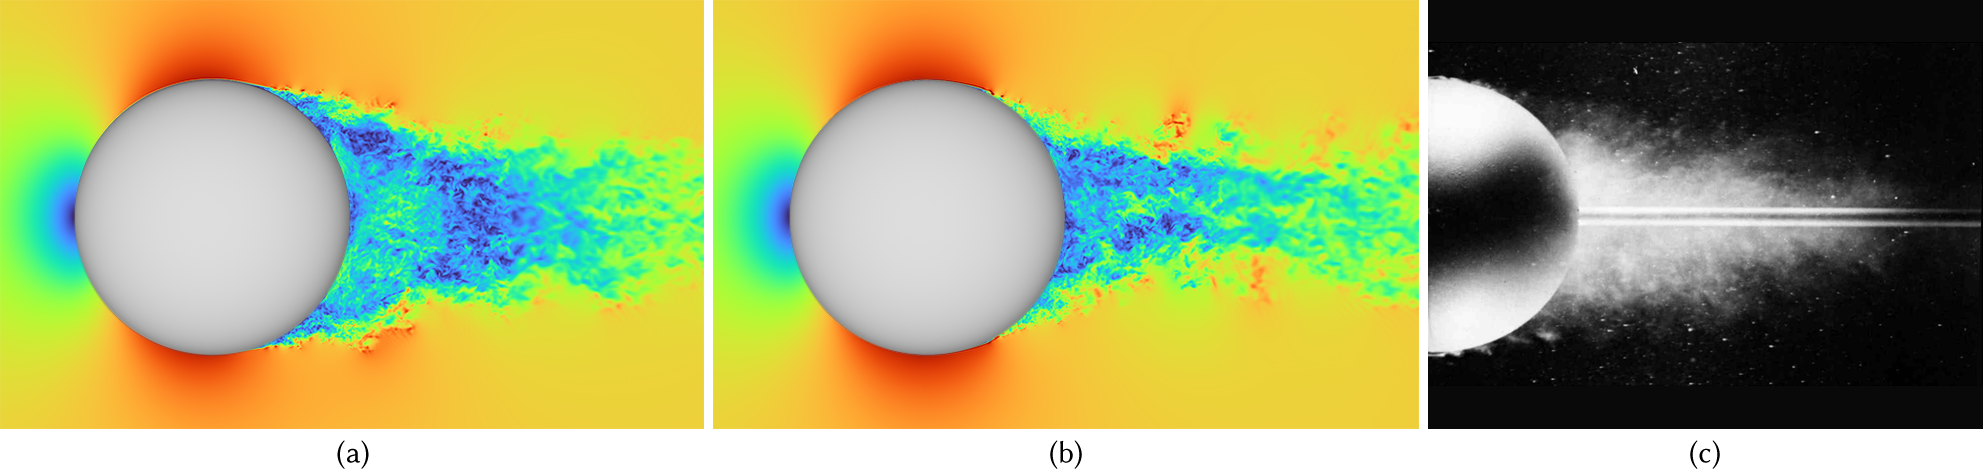
\includegraphics[width=0.99\columnwidth]{figures/wake_comp.png}
  \bicaption{球在发生阻力危机时的尾流。气流在$Re=400,000$下流过球时,由于固体边界附近的涡的尺度更小,尾流会收窄,从而阻力会下降。这一现象可见实际实验~\cite{Van-1982} (c)。与~\cite{Tao-2018-b} (a) 相比,在同样雷诺数下,我们的边界处理 (b) 捕捉到的边界的分离点更靠后,与实际实验更为接近。}{Wake of sphere in drag crisis. The flow passing through a sphere at $Re=400,000$ is known to exhibit in real-life experiment a narrower turbulent wake than at lower Reynolds numbers~\cite{Van-1982} (c) due to smaller scale vortices generated near the solid boundary, thus reducing drag significantly --- a paradox explained by the boundary-layer theory. Compared to~\cite{Tao-2018-b} (a), our improved boundary treatment scheme at the same Reynolds number (b) captures the separation point farther around the back of the sphere with a narrower wake, better matching the experimental visualization.}
  \label{img:sphere_wake_comp}
\end{figure}

\begin{figure}[htb]
\centering
  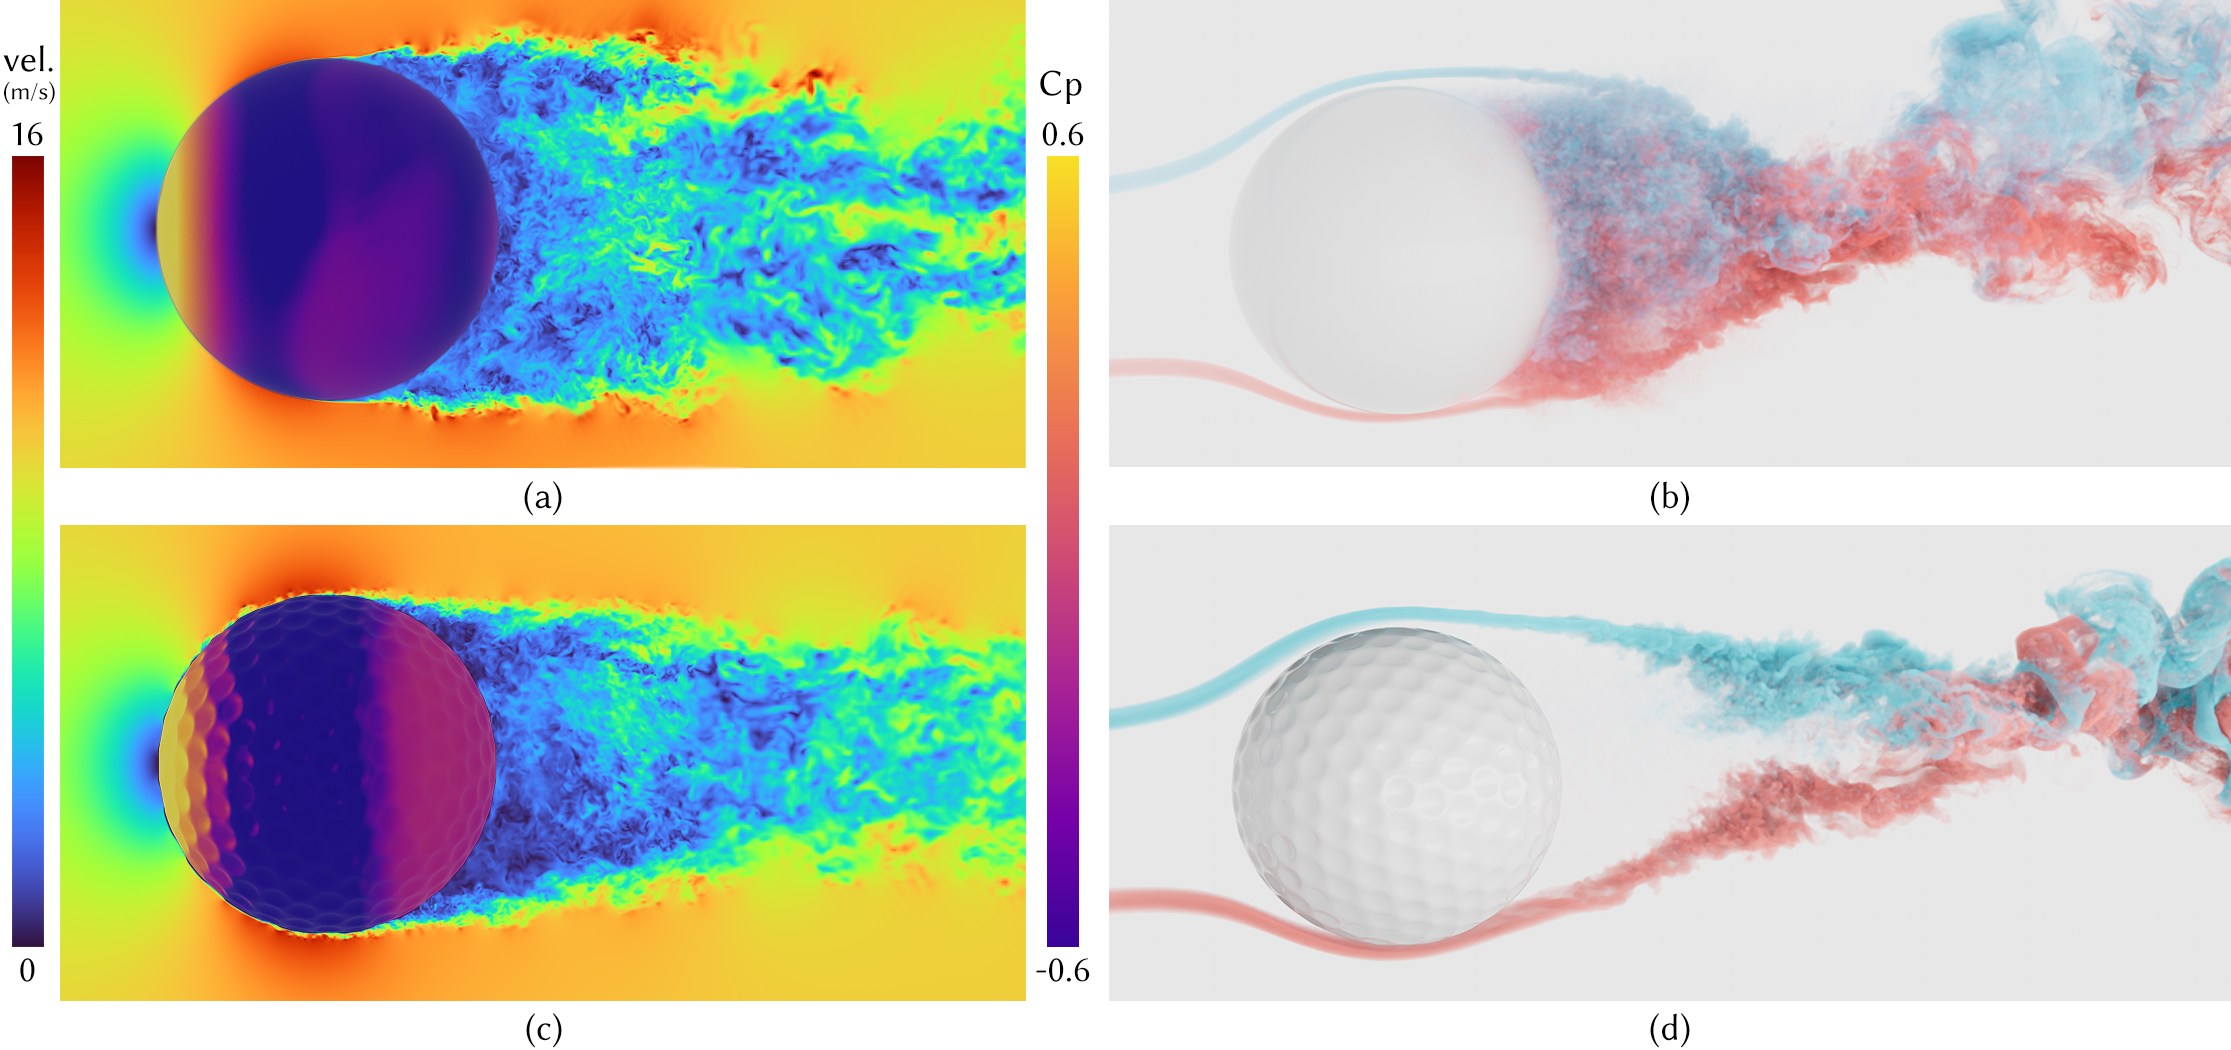
\includegraphics[width=0.99\columnwidth]{figures/golf_ball_vis.png}
\bicaption{光滑球与高尔夫球在Re=100,000时的对比。即使光滑球 (图中顶部子图) 与高尔夫球 (图中底部子图) 大小相同,只有表面的坑洞区别时,在我们的虚拟风洞测试中,也展现出完全不同的速度场与表面压力 ($C_\text{p}$) 场 (左图)。当我们使用染色粒子对流场进行被动追踪时,我们可以更清楚直观地看到这两者尾流所产生的区别 (右图),以理解为什么高尔夫球相对光滑球可以飞得更远。}{Ping-pong vs. golf ball at Re=100,000. While a ping-pong ball (top) differs (up to scale) from a golf ball (bottom) only in the absence of tiny dimples on its surface, testing these two balls in our wind tunnel exhibits very different velocity and surface pressure ($C_\text{p}$) fields (left); consequently, the flows visualized via passively-advected dyed particles are dramatically different (right), providing a good intuition of why golf balls can travel much further.}
\label{img:golf_ball_vis}
\end{figure}

\begin{figure}[htb]
\centering
  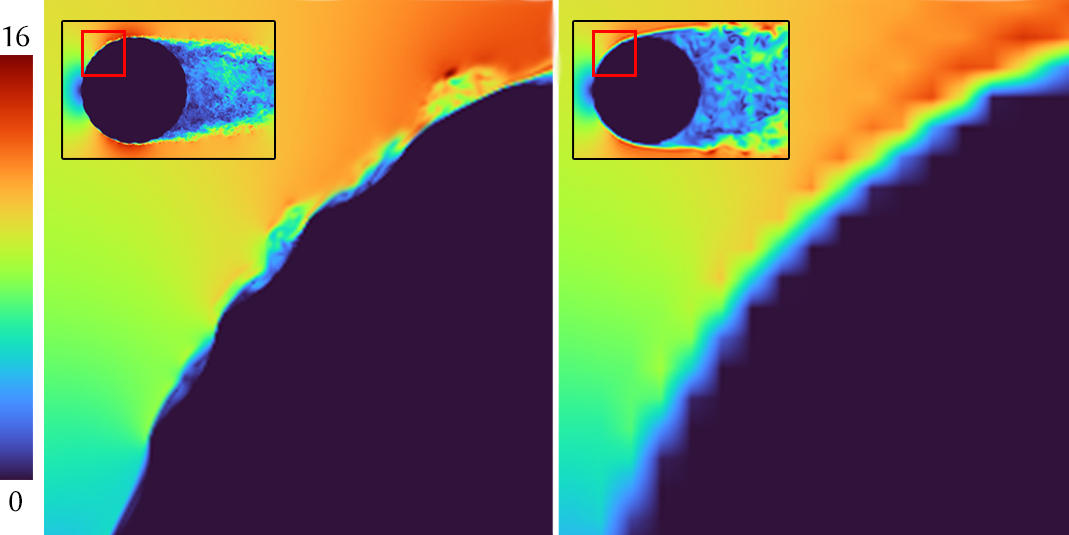
\includegraphics[width=0.99\columnwidth]{figures/golf_ball_single_res.png}
\bicaption{多分辨率网格与单分辨率网格仿真的对比。多分辨率网格可以对边界层有更准确的捕捉,在这个例子中可以将高尔夫球表面的小坑洞中的流体准确解算 (左图)。与总格点数相同的单分辨率网格 (右图) 相比,我们可以看到完全不同模式的湍流尾流。图中通过颜色可视化的为速度的模值,单位为$m/s$。}{Multi- vs. single-resolution simulation. A multiresolution simulation better resolves the boundary layer flow going within the small dimples of a golf ball (left), while a single-resolution simulation with the same total number of grid nodes cannot (right). As a consequence, we witness a very different behavior of the turbulent wake when the velocity magnitude (with a colormap indicating its value in $m/s$) is visualized.}
\label{img:golf_ball_comp_single_res}
\end{figure}

\paragraph{高尔夫球的气动特性}
我们还在虚拟风洞中测试了高尔夫在高速气流下的气动特性。我们使用的高尔夫球模型有$362$个坑洞 (美国职业高尔夫球巡回赛的赛事用球拥有最低322个,最高376个坑洞),坑洞深度与球的直径的比值为$0.007$。
如图~\ref{img:golf_ball_cd},我们通过仿真得到的阻力系数与已发表的实验数据~\cite{Bearman-1976, Aoki-2010}相吻合。这个结果同时可以验证我们的方法对于小尺度的几何变化的敏感性。在$Re\!=\!100,000$时,高尔夫球与表面光滑的球所造成的尾流截然不同。原因在于高尔夫球表面的小坑洞可以产生非常小的边界层涡流,并影响周围的流场,减小层流边界层在固体边界上的附着,这使得高尔夫球表面流场的分离点相比平滑球将更靠后,形成更加收窄的尾流形状,并降低自身阻力。这一点可见图~\ref{img:golf_ball_vis}。
注意我们的多分辨率网格是能捕捉到这样的小细节的关键。如果我们采用单分辨率网格,即使总网格数相同,也没有能力捕捉到高尔夫球表面坑洞所造成的薄边界层。这会造成仿真错误地预测边界分离点与尾流形状,并得到大幅升高的阻力系数,见图~\ref{img:golf_ball_comp_single_res} (右)。

\paragraph{DrivAer汽车模型的气动特性}
最后,我们对DrivAer汽车模型进行气动仿真。DrivAer汽车模型是慕尼黑工业大学 (Technische Universit\"at M\"unchen) 所制造的一个标准汽车测试模型,其主要目的是为了研究汽车外形对空气动力学特征的影响,同时验证数值仿真算法的能力~\cite{Heft-2011, Heft-2012}。这一模型在汽车工业受到广泛认可。
我们在测试中使用了三种不同的车型配置,三种配置的主要区别是汽车尾部的造型区别,分别被称为快背式 (fastback), 阶背式 (notchback) 与方背式 (estateback)。我们在测试中使用的模型的几何精度为3mm,带有发动机盖、轮胎、轮腔、后视镜与复杂底盘,且不考虑发动机舱内的流动。
所有的测试中,气流的流速 (即车速) 都被设置为$57.6 km/h$。并且,对每一个车型配置,我们都测试了有和无地面仿真 (ground simulation, GS) 这两种情况。在有地面仿真的情况中,地面的速度是与车速等同的,且轮胎也在以同样的线速度旋转。而没有地面仿真的情况中,地面和轮胎都维持静止。
这两种情况可以很直观地显示出,轮胎与地面的速度差别,对于风洞实验与气动结果的影响是巨大的。
我们将仿真得到的阻力数据画在了图~\ref{img:tum_validation_cd_curve} 中,这里阻力是随时间变化的。从图中可以看出,在流场经历过初始化带来的不稳定阶段后,阻力在约1 s后趋于稳定。我们将$1.2s$至$2s$区间内的阻力系数平均来得到相应车型配置的阻力系数,并于实际风洞实验值~\cite{Heft-2012b} 相对比,得到的结果可见表~\ref{tab:drivaer_result}。
注意我们的仿真结果是经过了一次平均值修正后的结果。平均值修正即我们将所有仿真结果与对应实验值误差的平均值减去,这样我们得到的可以认为是误差的变化趋势。这是工业设计中一个常见的做法。因为对于汽车这样的复杂模型,数值实验存在系统的偏差,包括我们之前讨论的地面与车身之间的流场,都会使计算得到的物理量发生整体的偏移。通过平均值修正我们可以弥补这种偏移。
图~\ref{img:fastback} 中展示了平均速度与压力场,平均的时间区间同样为$1.2s$至$2s$。图中分别展示了静止与旋转轮胎的表面压力,以显示有地面仿真和无地面仿真时的区别。
与我们的预想相一致,在没有地面仿真时,我们的方法精度更高,所得结果的误差平均约为$0.4\%$。这一结果远小于工业仿真中通常要求的$3\%$误差标准 (这一误差标准是我们与汽车制造商沟通获得的)。在有地面仿真时,我们的最大误差为$3.17\%$,也足以满足工业仿真中的需求 (在有地面仿真时,误差标准可以更宽容,一般在$5\%$)。

\begin{figure}[htb]
\centering
  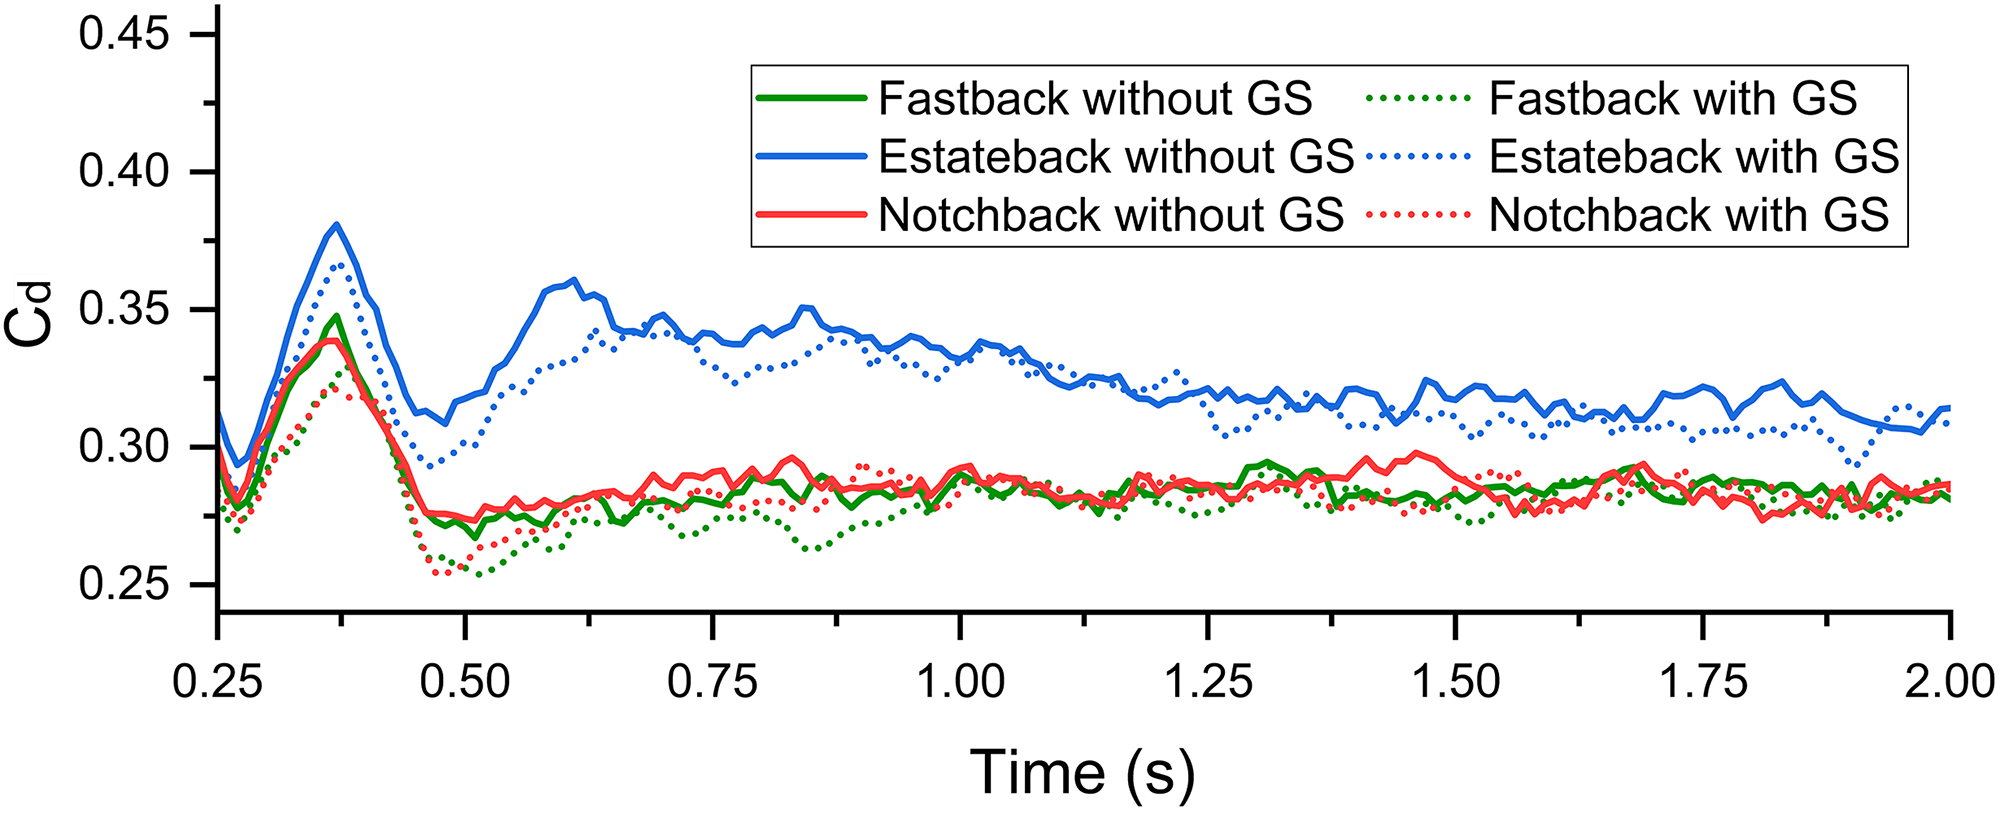
\includegraphics[width=0.99\columnwidth]{figures/tum_validation_cd_curve.png}
\bicaption{汽车的阻力随时间的变化。我们画出我们仿真所给出的不同DrivAer汽车配置的阻力系数随时间的变化,包括有地面仿真与无地面仿真的情况。(GS表示有地面仿真,即汽车的轮胎旋转且地面运动的速度与轮胎的线速度一致。)}{Car drag over time. We plot the simulated drag coefficient in time for different DrivAer car configurations, with or without ground simulation (GS, meaning ground motion and rotating wheels are simulated).}
\label{img:tum_validation_cd_curve}
\end{figure}

\begin{figure}[htb]
\centering
  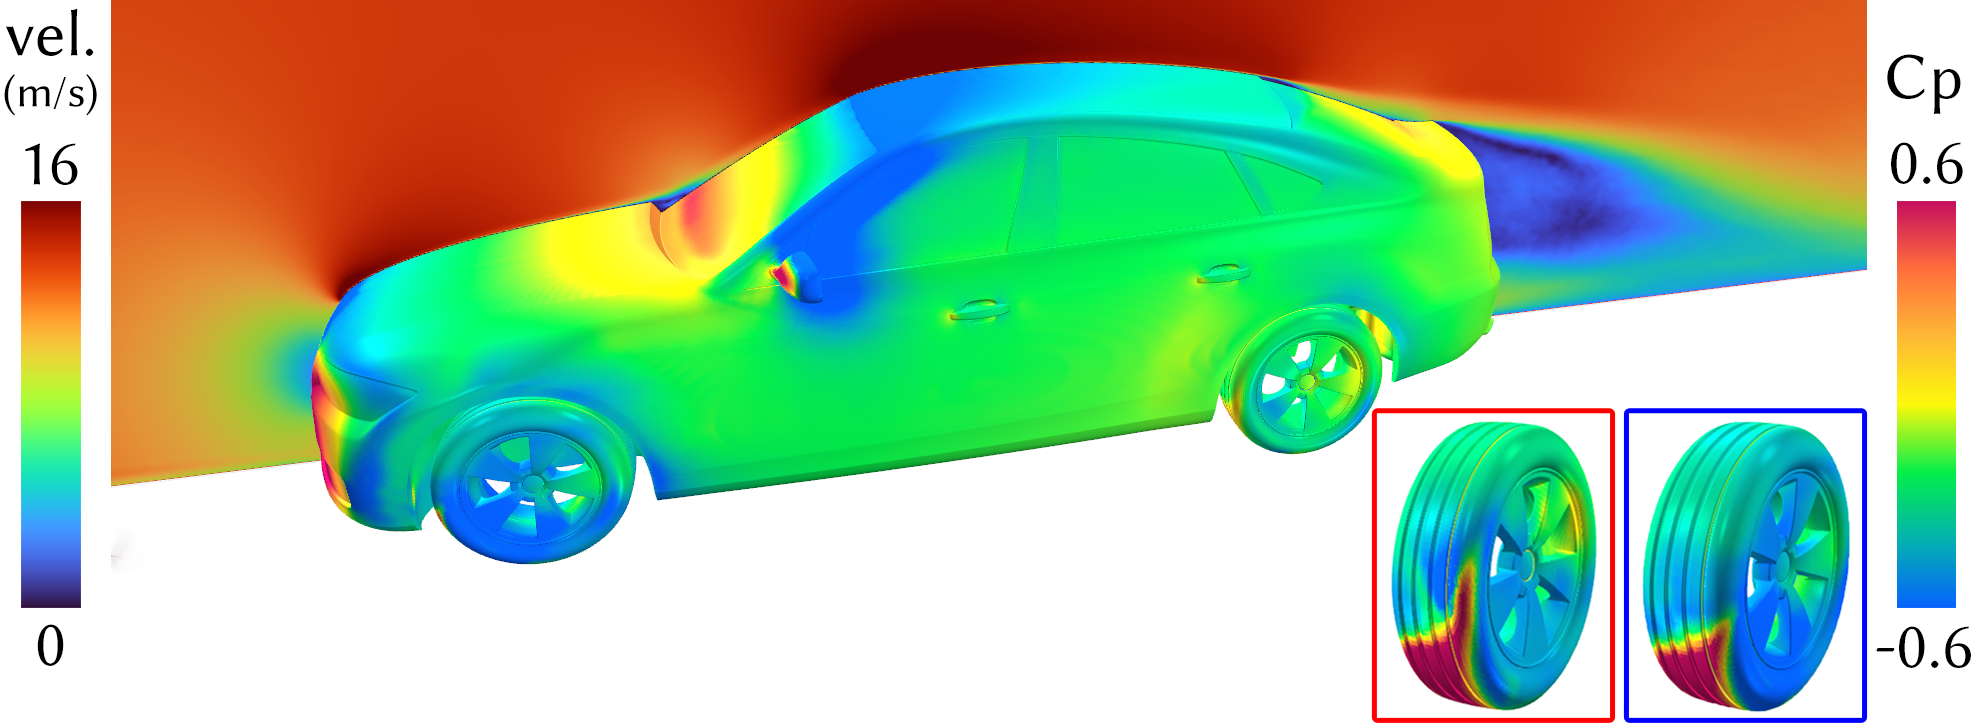
\includegraphics[width=0.99\columnwidth]{figures/tum_fastback.png}
\bicaption{DrivAer fastback汽车的空气动力仿真。我们对DrivAer fastback这样的标准测试车型进行气动仿真,图中展示了垂直的平均速度场截面,与模型表面的平均压力 (平均均指随时间平均)。轮胎在有地面仿真 (蓝色方框内) 与无地面仿真 (红色方框内) 时的平均表面压力可视化也在图中展示。}{DrivAer Fastback aerodynamic simulation.
A vertical cross-section shows the magnitude of the mean velocity flow around the DrivAer fastback benchmark car model, while the mean pressure over the model surface colors the mesh.
Mean pressure distributions without (red inset) and with (blue inset) ground simulation are also visualized on the wheels.}
\label{img:fastback}
\end{figure}

\paragraph{与现有工业软件的对比}
前文中曾提到过,西门子 (Siemens) 的StarCCM+~\cite{Siemens}与达索 (Dassault Syst{\`e}mes') 的PowerFLOW~\cite{powerflow}是两个被广泛使用的商业流体仿真分析软件,并分别通过基于FVM的N-S求解器与LBM求解器实现流体仿真。两者一般都运行于CPU集群环境。
因为StarCCM+在进行非稳态仿真时,计算量非常大,仿真时间可达数周,所以StarCCM+更经常被用于稳态求解。而稳态求解的问题是,如面对轮胎旋转这样的场景时,边界必须采取一定的近似。这与实际的物理情况并不相符。PowerFLOW克服了这些问题,但是只能在CPU集群上使用限制了LBM方法的并行优势。
而我们的方法既继承了动理学方法的优势 (即PowerFLOW软件的优势),同时又可以在GPU上解算,使得硬件需求大幅下降。如我们使用NVIDIA A100 GPU (拥有6,912个CUDA核) 对DrivAer的快背式模型进行2s的仿真,在没有地面仿真时只需约3个小时即可完成仿真,即每秒的仿真需要10,356 GPU核时。
James等~(\citeyear{James-2018}) 使用PowerFLOW与StarCCM+分别对DrivAer的方背式模型进行了类似的仿真。在结果达到收敛时,PowerFLOW的仿真在96个CPU的集群上需要约80小时,StarCCM+在128个CPU的集群上需要约13小时。
假设上述CPU拥有至少8个核心的情况下,通过计算我们可以得知在核数相当时,我们的方法是更高效的。当然因为CPU平台与GPU平台直接比较性能是很困难的,我们这里只非常定性地对效率进行了描述。
此外,更引人注目的是,在James等~(\citeyear{James-2018}) 所报告的PowerFLOW的计算结果中,并没有显示出有地面仿真与无地面仿真时,阻力系数有明显区别。这与实验数据相违背。其它的结果与实验值~\cite{Heft-2012b} 相对比时,大约均在3\%的误差水平。
我们需提请注意的是,在该工作中,作者使用了没有后视镜的模型,而我们使用了带有后视镜的模型。此外作者没有提供任何数值修正相关的信息。
这证明了在DrivAer测试中,精度层面上,我们与现有的工业软件是大致相当的。当然我们也认为我们需要与PowerFLOW与StarCCM+等软件进行更直接的对比,以更明确地确定我们的方法与现有工业软件的优劣。这些我们留在未来的工作中。

\begin{table}[htb]
  \centering
\bicaption{DrivAer汽车模型的阻力计算精度。我们对我们仿真得到的不同DrivAer车型配置的阻力系数$C_\text{d}$与实验值进行了比较。GS表明地面仿真,即有GS时地面运动且轮胎旋转。}{Drag estimation accuracy of DrivAer car model. We compare our estimates of the drag coefficient $C_\text{d}$ for different DrivAer configurations with experimental data, with or without ground simulation (GS, meaning ground motion and rotating wheels are simulated).}
\begin{tabular}{*{4}{c}}
      \toprule
  车型配置 & 仿真所得$C_\text{d}$ & 实际实验所得$C_\text{d}$ & 相对误差 \\
      \midrule
  快背式 (无GS) & 0.2849 & 0.284 & 0.32\%\\
  阶背式 (无GS) & 0.2851 & 0.286 & -0.31\%\\
  方背式 (无GS) & 0.316 & 0.318 & -0.63\%\\
  快背式 (有GS) & 0.2811 & 0.275 & 2.22\%\\				
  阶背式 (有GS) & 0.283 & 0.277 & 2.17\%\\				
  方背式 (有GS) & 0.3089 & 0.319  & -3.17\%\\
      \bottomrule
\end{tabular}
\label{tab:drivaer_result}
\end{table}

\section{面向视觉动画的仿真结果}
\paragraph{与实际实验的对比}
为了进一步验证我们方法在有亚网格物体时边界处理的精度,我们与现实世界中的实验进行对比。
首先我们与三角翼的风洞实验进行比较。该三角翼的后掠角度为$75^\circ$,攻角为$20^\circ$ (见图~\ref{img:comparison_delta_wing} (a))。在实验中,三角翼上方会产生稳定的螺旋涡流结构,提升气动升力 (这种升力被称为涡升力~\cite{anderson2010aircraft})。这种结构被广泛使用于现代飞行器的设计中,如图~\ref{img:teaser_concorde} 中的协和客机。该实验的可视化可见图~\ref{img:comparison_delta_wing} (b)~\cite{Delery:2001}。我们的仿真结果在视觉上与实验结果相匹配,展示出相似的螺旋涡流结构。除去这一定性的对比实验,我们还对旋翼的气动性能进行了定量分析。我们参照一项最近的专利~\cite{lin2020screw} 中的描述重建了旋翼模型,并测量旋翼在旋转时的推力 (计算方法参照~\cite{leishman_2016}),与专利中的数据对比。图~\ref{img:DJI_thrust_compare} (a) 展示了不同转速下的计算误差,显示出较好的一致性。值得注意的是,随着转速的提升,相对误差会升高。这一点的主要原因是在LBM中,随着参照速度的提升,LBM空间下黏度在不断减小,以至于我们在测试时使用的32位浮点数已无法有效保证碰撞过程的计算精度。我们还对收敛性进行了测试,即在固定转速下提升分辨率,结果可见图~\ref{img:DJI_thrust_compare} (b)。这一结果显示了我们方法误差随分辨率的收敛性。

\begin{figure}[!htbp]
  \centering
    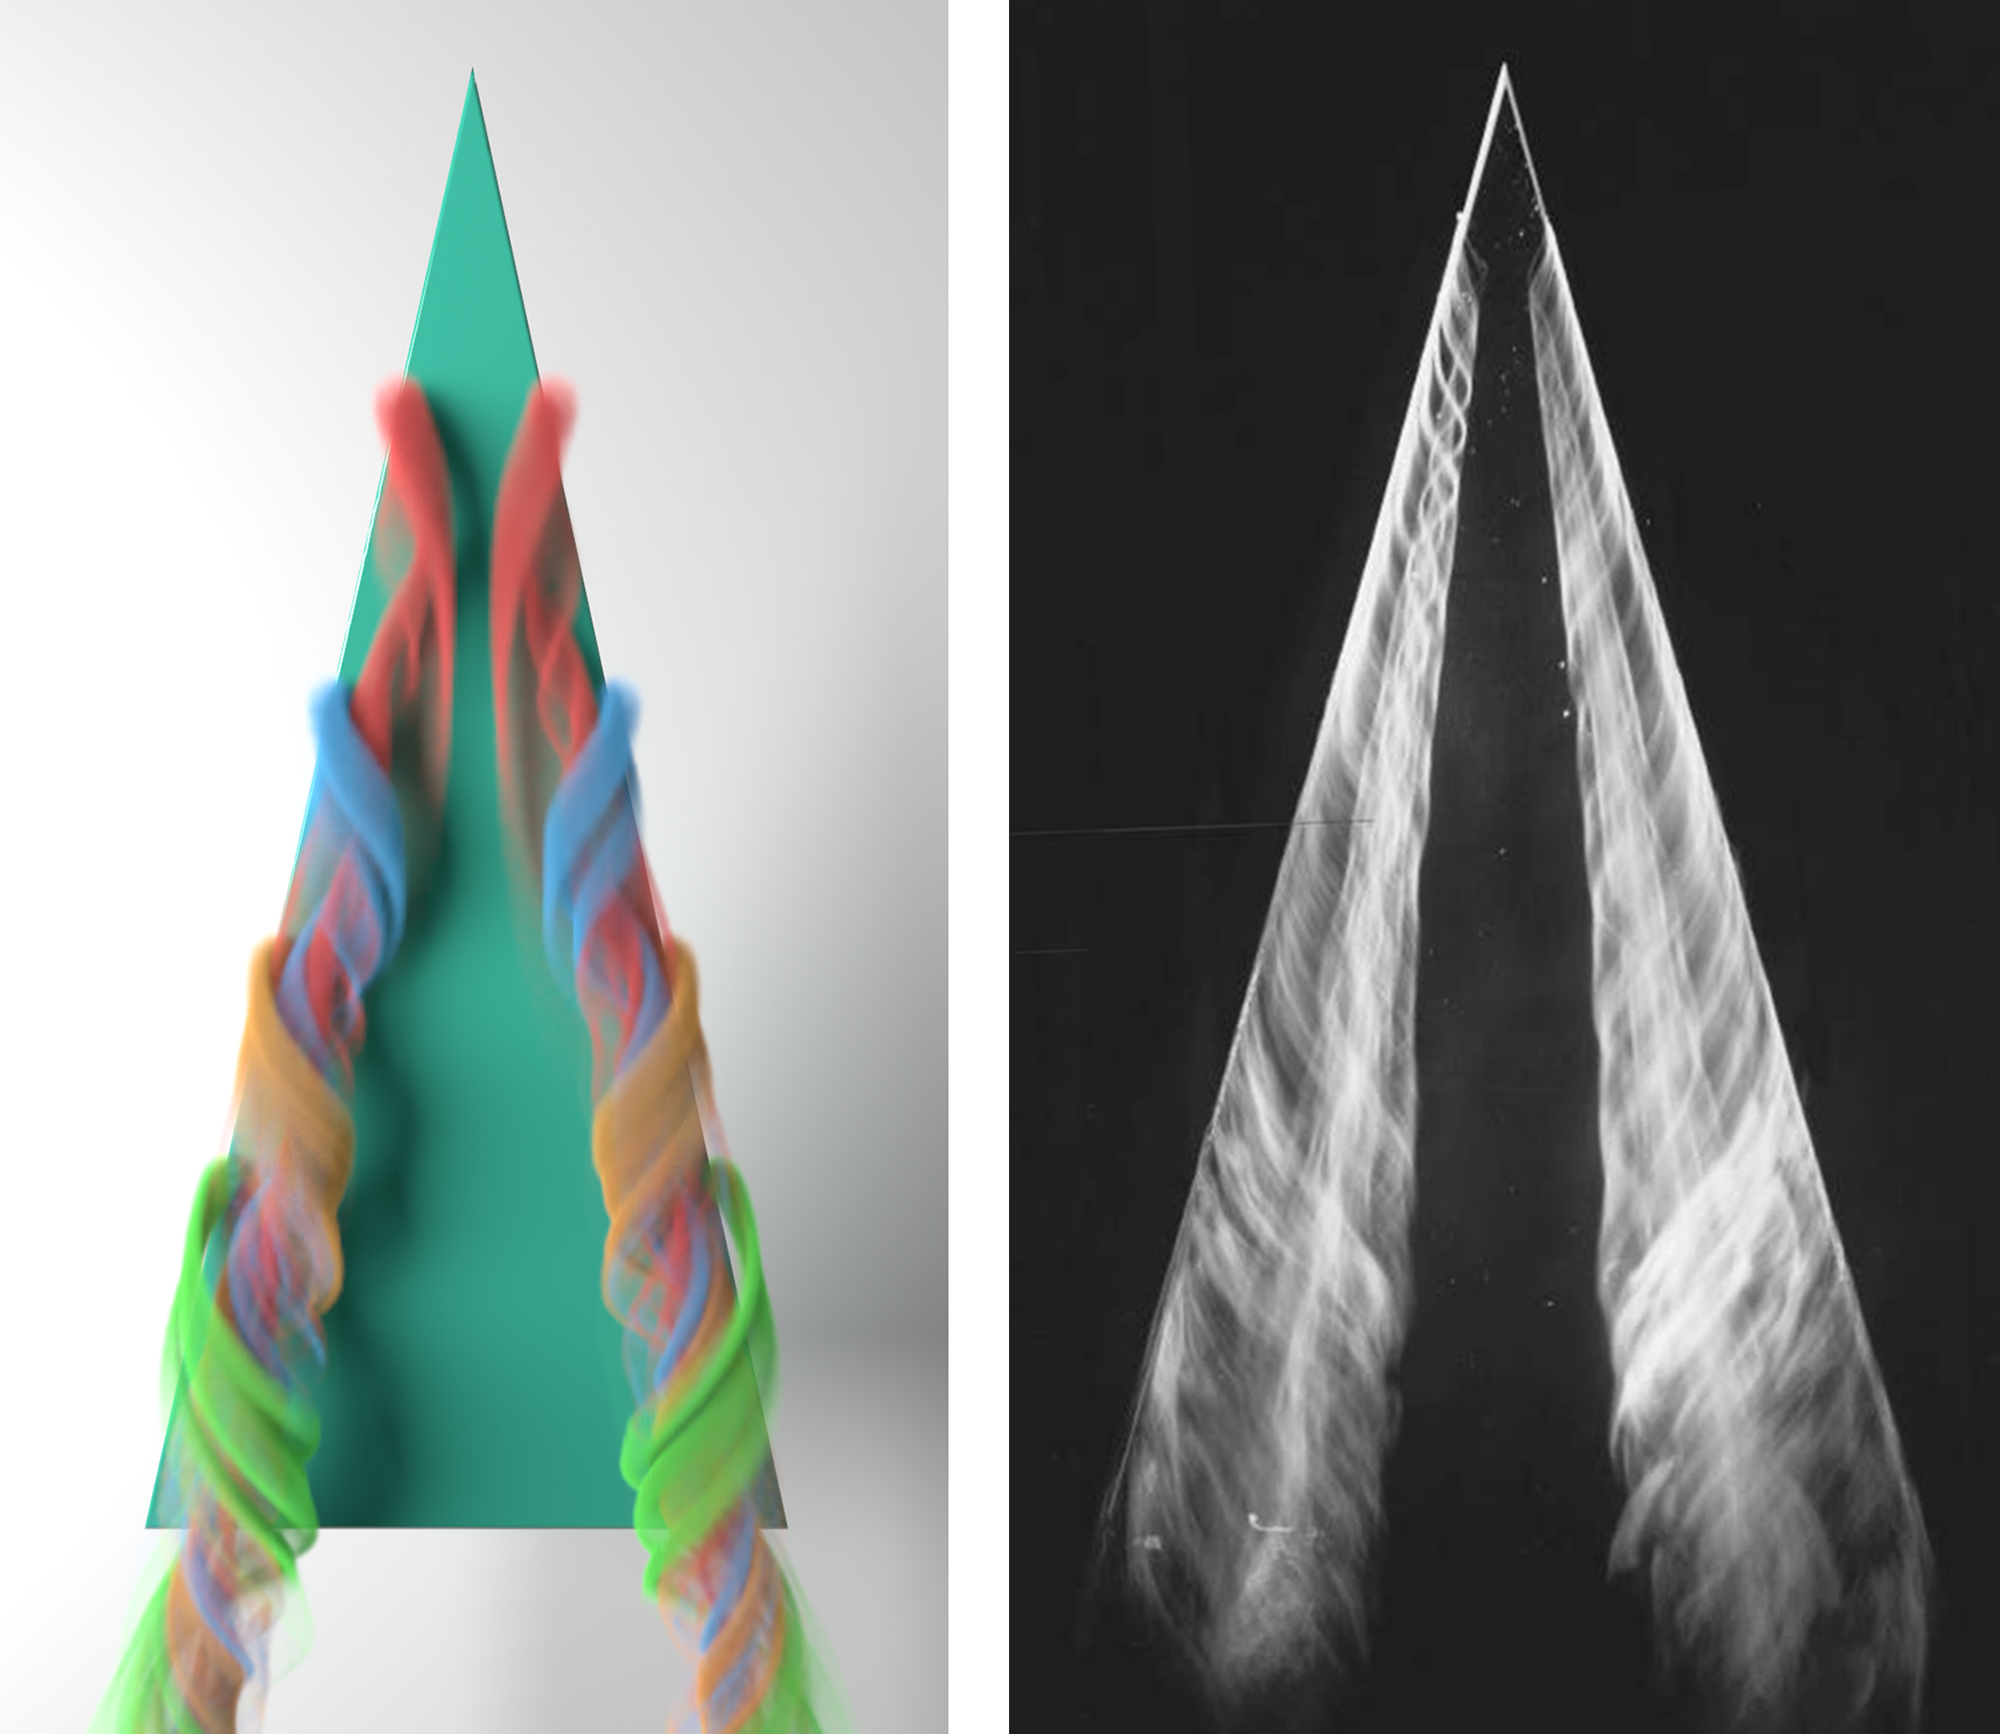
\includegraphics[width=0.99\columnwidth]{figures/comparison_delta_wing.png}
  \bicaption{三角翼仿真。通过我们的图形方法得到的薄板三角翼仿真结果 (左图) 与实际实验~\cite{Delery:2001} (右图) 的对比,展示出相同的前缘涡旋结构,表面我们的图形方法在薄结构边界层上的准确性。}{Delta-wing simulation. The airflow over a thin-shell delta-wing simulated with our hybrid coupling approach (left) matches experimental visualizations from~\cite{Delery:2001} (right), exhibiting the same spiral vortex structure near the leading edge of the wing and demonstrating the accuracy of our solver in capturing boundary layer flows around thin structures.}
  \label{img:comparison_delta_wing}
\end{figure}

\begin{figure}[!htbp]
  \centering
    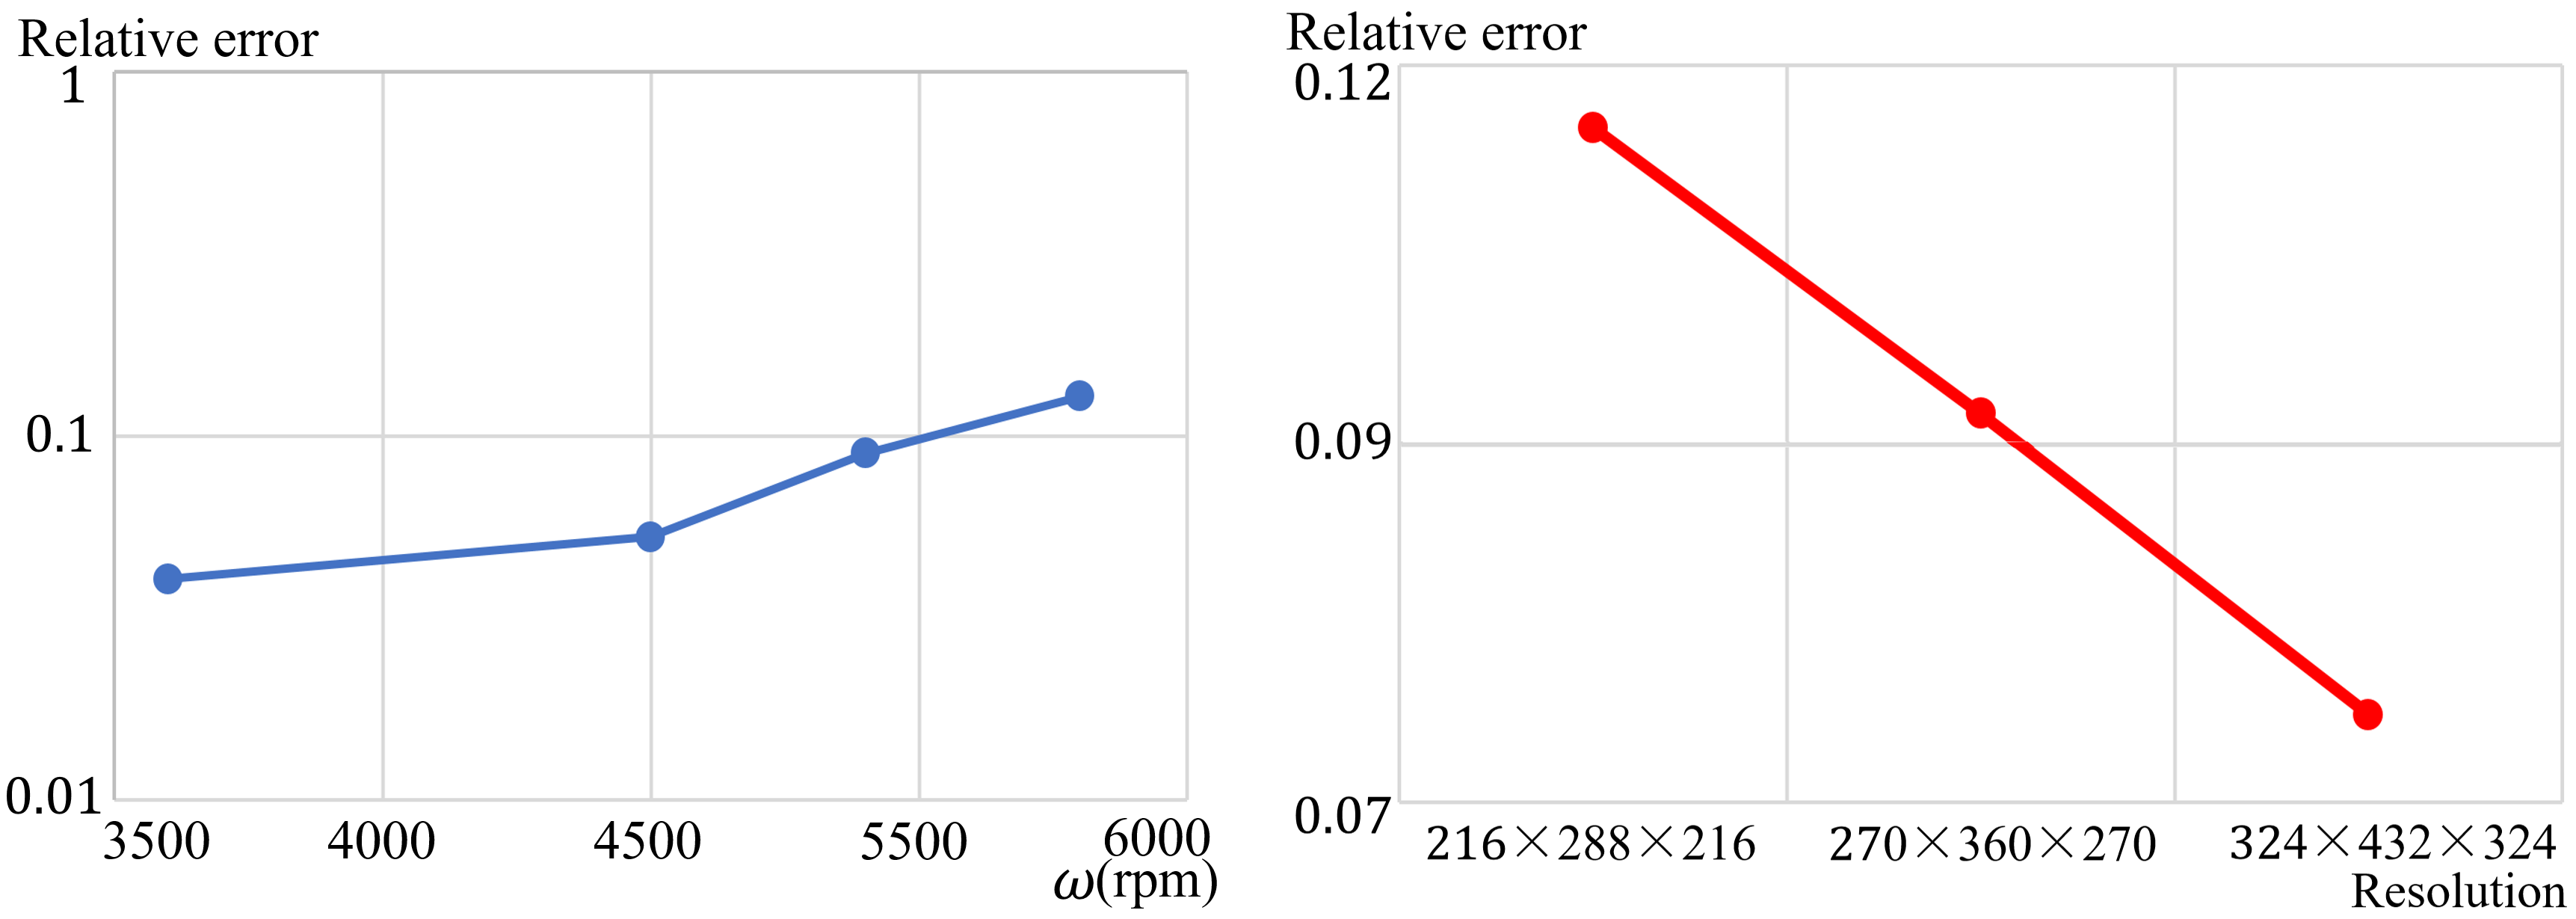
\includegraphics[width=0.99\columnwidth]{figures/DJI_compare.png}
  \bicaption{推力的验证。我们通过旋翼旋转的气动仿真来测试旋翼的推力。我们在$288\!\times\!324\!\times\!288$分辨率下测试不同转速的误差结果见左图。右图为固定3600 rpm转速时,相对误差的收敛情况。注意我们采用的分辨率并不是非常高,所以结果的精度依然有提升空间。}{Thrust evaluation. From the simulation of the coupling between a rotating drone blade and the surrounding air, we can compute the estimated thrust values at different rotation speeds with a grid resolution of $288\!\times\!324\!\times\!288$ (left). The relative errors of our thrust value at 3600 rpm w.r.t. experimental measurements as the grid resolution increases (right) indicates convergence of our solver. Note that the tested grid resolutions are not very high, and more accurate results are expected for higher grid resolutions.}
  \label{img:DJI_thrust_compare}
\end{figure}

下面我们展示一系列的仿真结果。这些仿真结果都于一个14核Intel Xeon E5-2690 CPU、128 GB内存、NVIDIA RTX 3090的工作站上运行得到。我们通过一系列的单向与双向流固耦合算例,对一系列的复杂几何进行测试,以显示我们的方法处理不同类型物体的能力。我们还展示了一些可交互的仿真、与离线的高分辨率大规模仿真。

\begin{figure}[!htbp]
  \centering
    \includegraphics[width=0.99\columnwidth]{figures/result_tube.png}
  \bicaption{旋转的薄圆柱面。一个薄圆柱面分别在高黏度 (顶图) 与低黏度 (底图) 流体中绕轴旋转。在圆柱面内部和外部分别有烟雾粒子对流场进行可视化 (内部为蓝色,外部为红色)。左图与右图分别展示仿真在4s与7s后的烟雾形态。}{Rotating cylindrical thin shell. A cylindrical thin shell rotating around its axis in a very high (top) and very low viscosity (bottom) fluid respectively, where smoke particles scattered inside (blue) and outside (red) the thin-shell cylinder are advected in the flow (left: after 4 seconds; right: after 7 seconds) to demonstrate that boundary layers are well resolved.}
  \label{img:result-tube}
\end{figure}

\begin{figure}[!htbp]
  \centering
    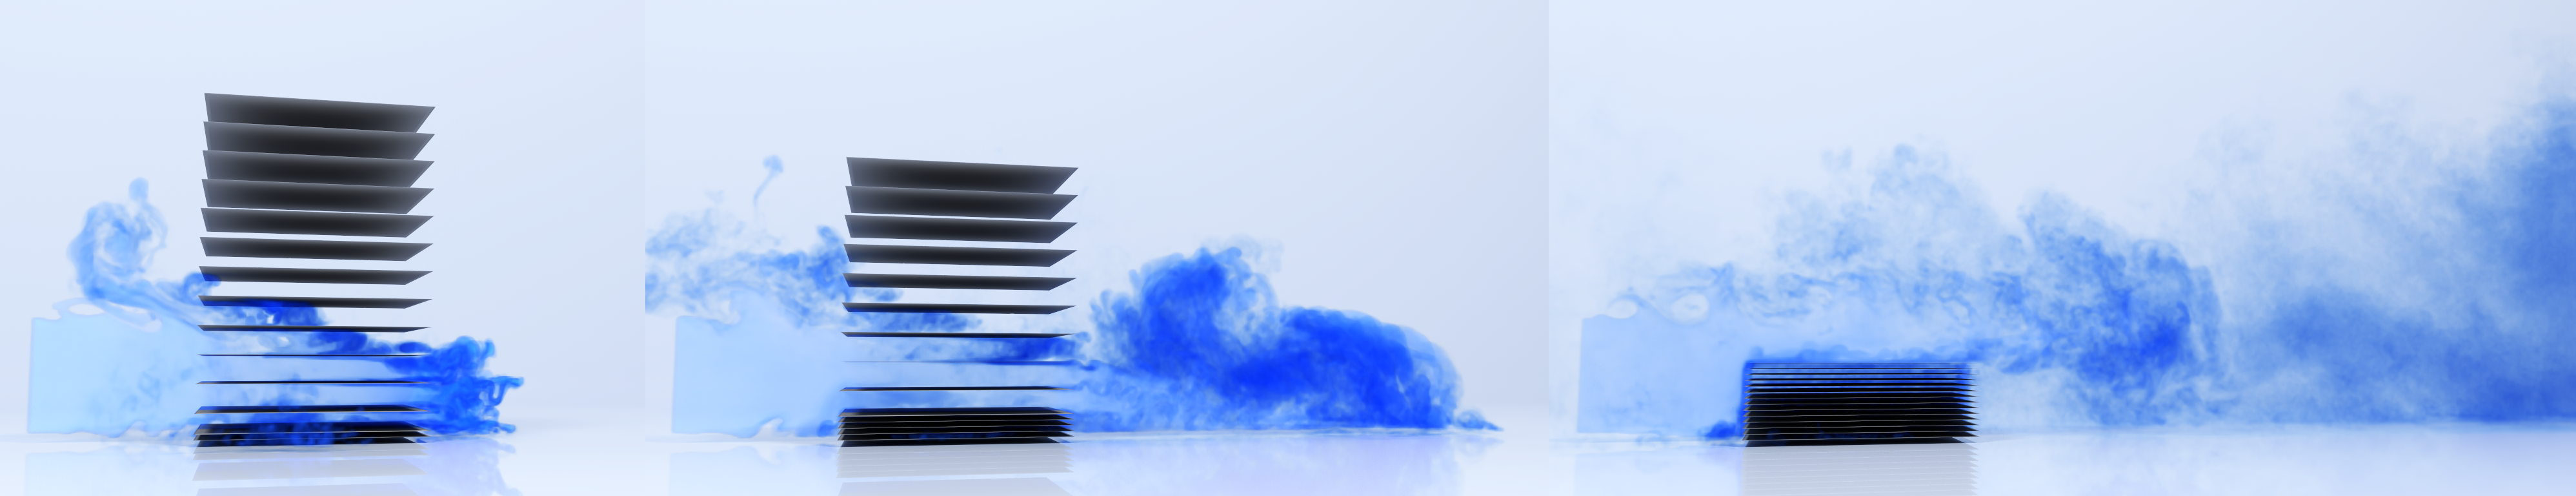
\includegraphics[width=0.99\columnwidth]{figures/result_thin_shell_sub_grid.png}
  \bicaption{烟雾经过层叠的板子。烟雾吹过一系列下落的薄板。虽然薄板在分开时烟雾可以通过,当它们层叠在一起时却形成一个密闭的障碍物。我们边界处理中的亚网格近似可以同时处理这两种不同情况,当板子加速靠近时,中间的流体会被加速,而它们紧贴时会成为一个厚的物体。}{Smoke flow through stacked plates. Smoke is blown towards a falling stack of thin plates. While smoke freely flows between separate plates, they become an airtight obstacle when they are stacked on top of each other. Our boundary treatment based on subgrid approximation deals with both cases seamlessly: plates getting closer accelerate the flow in between them, while tightly stacked plates are treated as thick solids.}
  \label{img:result-thin-shell-sub-grid}
\end{figure}

\begin{figure}[!htbp]
  \centering
    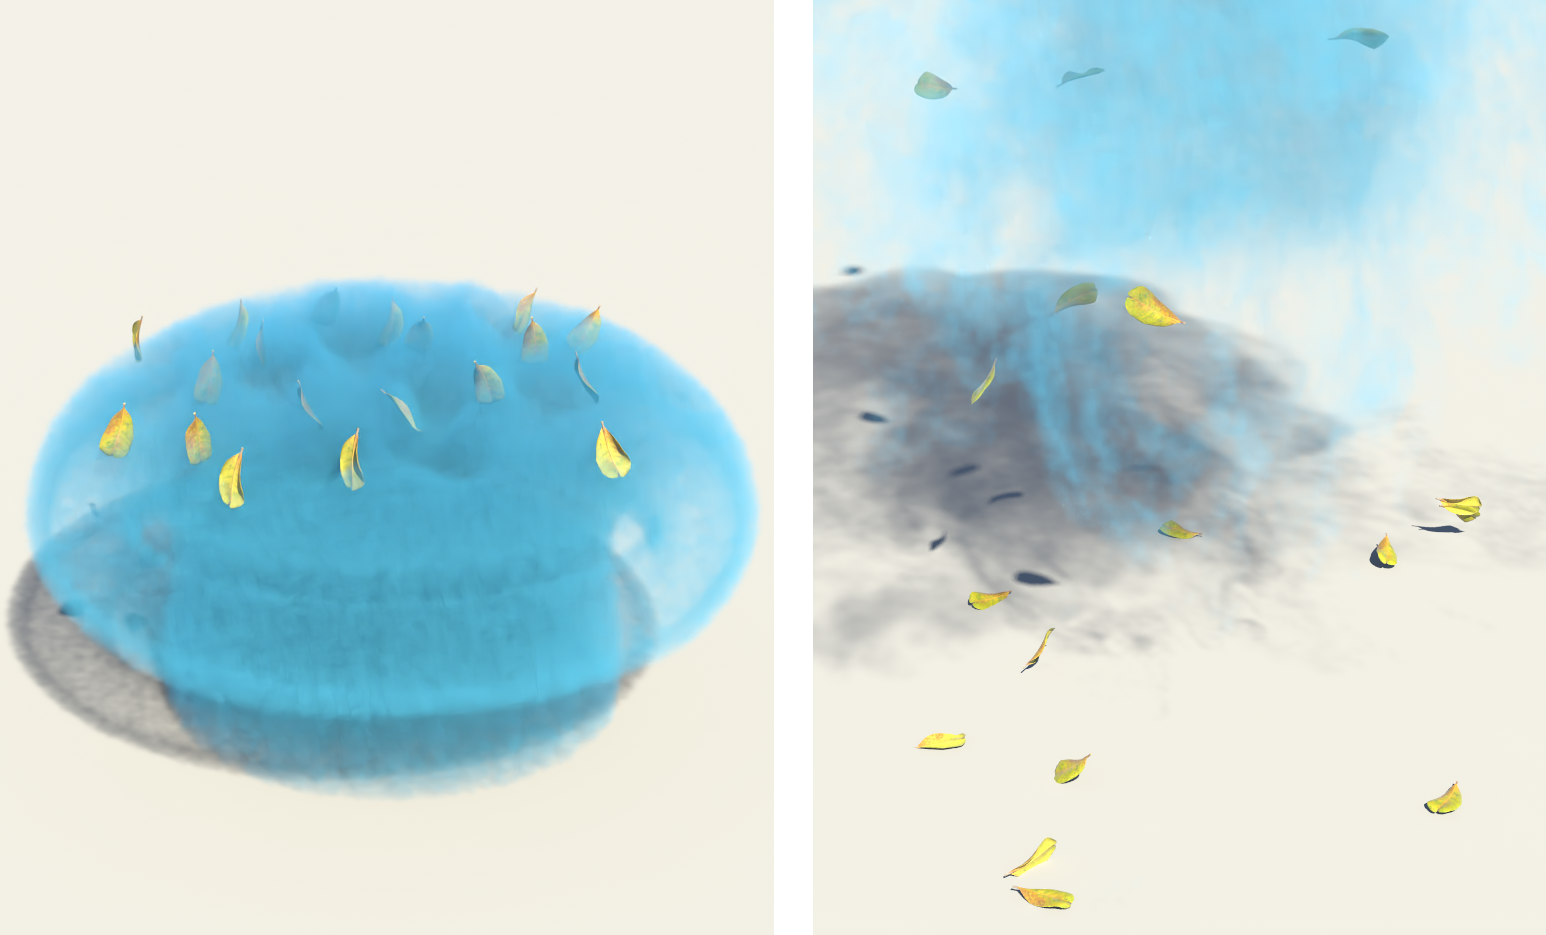
\includegraphics[width=0.99\columnwidth]{figures/result_blowing_leaves.png}
  \bicaption{风吹叶子的仿真。在这个双向流固耦合结果中,一阵风从地面吹起将树叶吹向空中。}{Wind blowing leaves. In this two-way coupling example, a puff of wind from the ground drives a bunch of dried-up leaves up in the air.}
  \label{img:result-blowing-leaves}
\end{figure}

\paragraph{与薄板的耦合}
我们首先构造一个薄圆柱面,使得厚度远小于网格大小,之后令圆柱面旋转,产生剪切流 (见图~\ref{img:result-tube})。我们在低雷诺数 (高黏度) 与高雷诺数 (低黏度) 分别进行了测试,并展示出完全不同的流场特性。我们还测试了多个薄板相叠的算例。这些薄板最初是分开的,之后逐渐叠落在一起。我们的亚网格近似使得我们的方法可以仿真从起初分离的薄板到叠在形成一个固体的整个过程,而无需任何调整。结果可见图~\ref{img:result-thin-shell-sub-grid}。我们最后展示一个双向耦合的结果,仿真一阵风从地面吹起树叶的过程。树叶一开始被风吹起后,缓慢地落回地面,并因风产生旋转。结果可见图~\ref{img:result-blowing-leaves}。

\begin{figure}[!htbp]
  \centering
    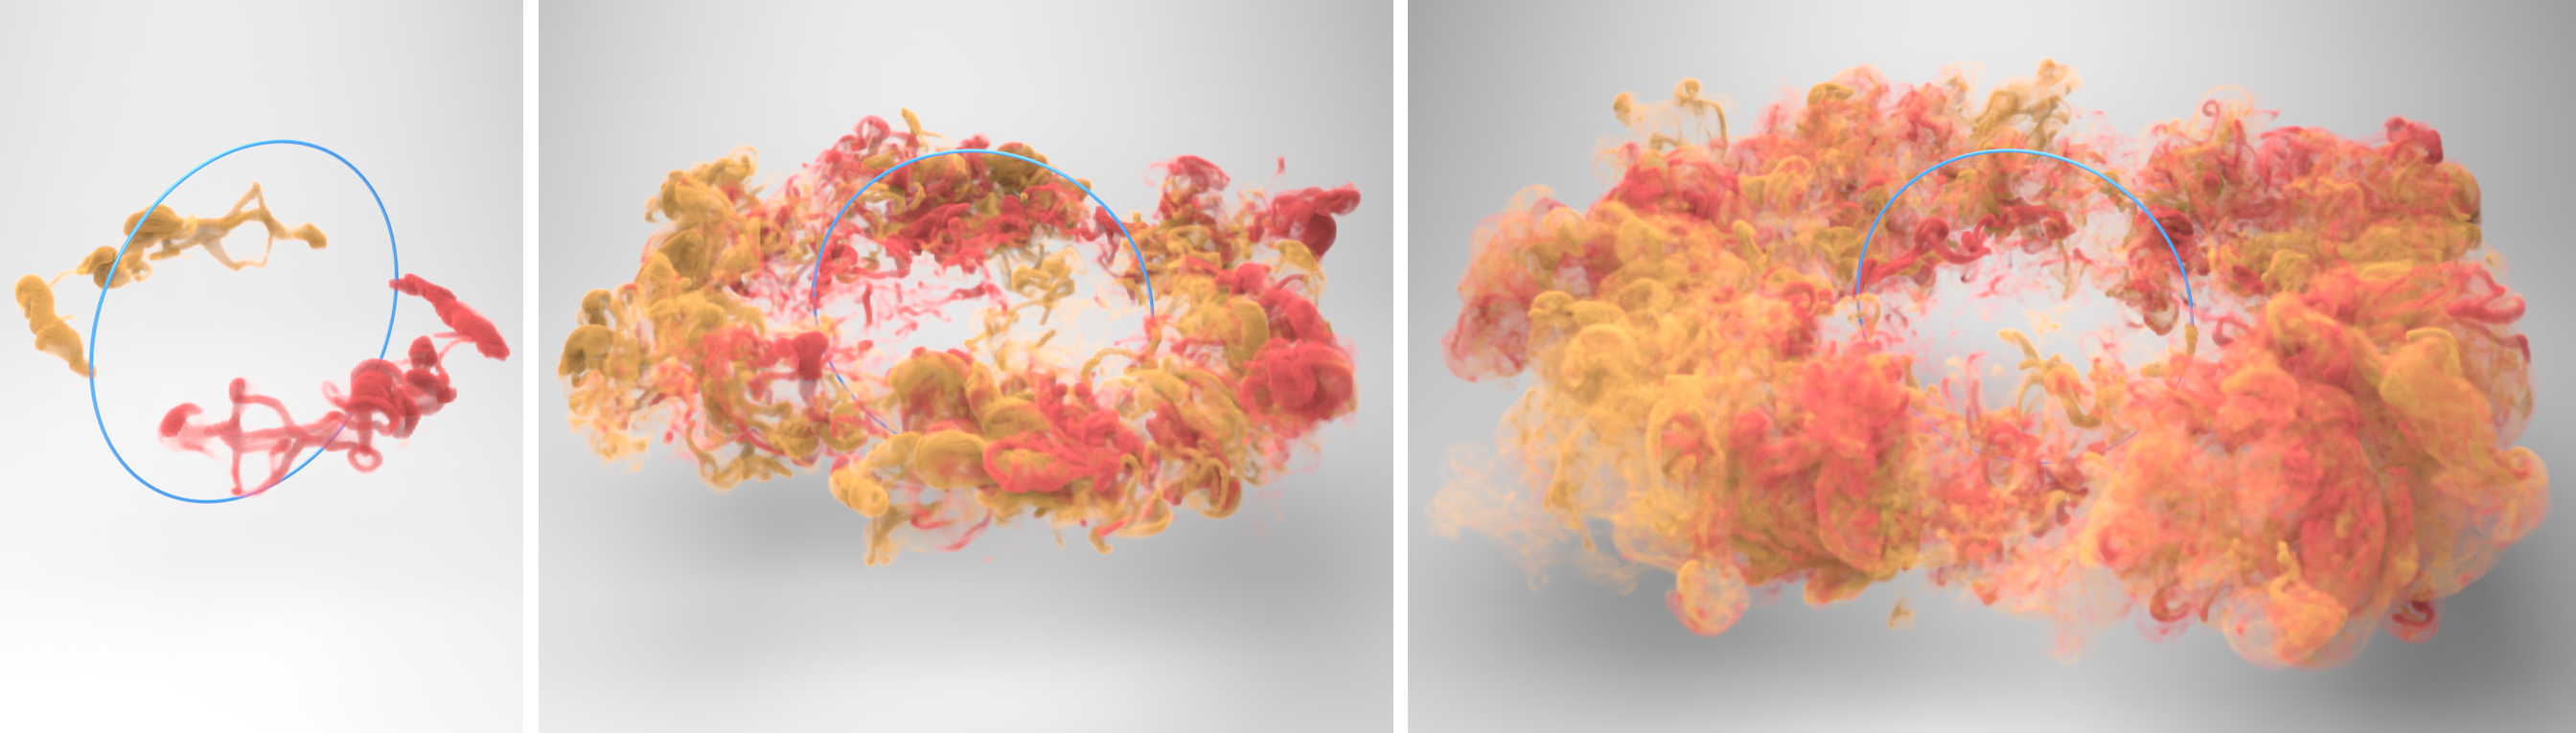
\includegraphics[width=0.99\columnwidth]{figures/result_rotating_torus.png}
  \bicaption{旋转的圆环。一个非常细的圆环沿着一个垂直轴旋转,在两侧发出黄色和橘色的烟雾,展示出圆环旋转所带出的湍流。}{Rotating ring. A very thin ring rotating along a vertical axis and emitting yellow and orange smoke particles is enough to create a turbulent wake as evidenced by the volutes of smoke resulting from the motion.}
  \label{img:result-rotating-torus}
\end{figure}

\begin{figure}[!htbp]
  \centering
    \includegraphics[width=0.99\columnwidth]{figures/result_thin_rod_sub_grid.png}
  \bicaption{发梳仿真。一个包含着上百根硬毛地发梳 (左图) 在旋转的同时从左向右平移,带动周围气流运动。与有硬毛的情况 (右图) 相比,没有硬毛时的发梳 (中图) 运动产生的尾流更加平滑,涡旋也更大。这个结果展示了我们的边界处理方法,包括亚网格近似,处理复杂几何的能力。}{Hair brush. The translating and rotating motion of a hair brush containing hundreds of bristles (left) creates fine vortices in its wake as well as around the bristles (right) as evidenced by the evolution of the smoke passing around it, properly capturing the intricate fluid-solid interaction engendered by this complex geometry. Compared to the coupling with bristles (right), the smoke near the hair brush without bristles (middle) is much smoother, and the wake flows contain relatively large vortices, indicating the efficacy of subgrid approximation in handling such complex solid shapes.}
  \label{img:result-thin-rod-sub-grid}
\end{figure}

\paragraph{与细棒的耦合}
下面继续展示我们的求解器对细棒耦合的仿真结果。我们先展示一个环状物体在空气中定速旋转的结果,其直径远小于网格大小,见图~\ref{img:result-rotating-torus}。我们还对多个细棒组合在一起时的情况进行仿真,结果见图~\ref{img:result-thin-rod-sub-grid}。注意当固体表面有硬毛时,尾流的湍流程度有显著的差别。

\begin{figure}[!htbp]
  \centering
    \includegraphics[width=0.99\columnwidth]{figures/result_wind_turbine.png}
  \bicaption{风力涡轮机的仿真。常速的风吹过一个有三个扇叶的风力涡轮机,驱动涡轮机旋转,并由扇叶上产生的烟雾对涡旋尾流结构进行可视化。这个双向的流固耦合结果考虑了轴上的摩擦力来限制了最大的角速度。扇叶角速度随时间的变化可见底部的小图。}{Turbine. A large turbine emitting colored smoke particles at the three propellers of its large blade is simulated with a constant incoming air flow making it turn, creating a spiral vortex trail. This two-way coupling example also involves friction on the axis of the turbine to limit its maximum angular velocity, resulting in a time-varying but converging curve of angular velocity of the turbine shown in the bottom inset.}
  \label{img:result-wind-turbine}
\end{figure}

\begin{figure}[!htbp]
  \centering
    \includegraphics[width=0.99\columnwidth]{figures/teaser_concorde.jpg}
  \bicaption{飞机气动仿真。通过对协和客机翼面的气流仿真,我们展示出我们的方法可以同时处理含有薄板、细棒的薄物体以及厚物体的复杂几何。}{Aerodynamic simulation of an airplane. By simulting the flow over the wing of the Concorde airplane, we demonstrate that our method can handle complex solids containing thin shells, rods and thick objects.}
  \label{img:teaser_concorde}
\end{figure}

\paragraph{与复杂物体耦合}
一个更复杂但非常常见的情况是厚物体与薄物体同时存在,并共同构成一个复杂物体。我们的边界处理可以有效并统一地处理这种情况。图~\ref{img:result-wind-turbine} 展示了通过风带动一个三扇叶风力涡轮机模型旋转的仿真结果。这里风在带动扇叶旋转的同时,扇叶也影响空气流动,展现了我们方法处理复杂物体的双向耦合。图~\ref{img:teaser_concorde} 展示了协和式客机以攻角20度姿态在空中飞行的仿真结果。对于飞机这样的复杂物体,许多部件对于网格都是亚网格大小的,尤其是机翼部分。在这两次仿真中,得到的结果都与期望相符。

\begin{figure}[!htbp]
  \centering
    \includegraphics[width=0.99\columnwidth]{figures/result_design.png}
  \bicaption{快速交互设计。我们通过GUI操作模拟系统,来快速生成仿真结果。图中示例为一个快速旋转的旋翼,我们可以通过可视化即时的看到尾流情况。这样的快速交互式仿真可以用来辅助产品设计与验证。}{Fast simulation for interactive design. We operated our GUI-based simulation system to produce a quick preliminary result of a fast rotating rotor-blade where turbulent wake flows can be observed interactively, which is very useful for efficient product design and verification.}
  \label{img:result-design}
\end{figure}

\paragraph{快速仿真以进行交互式设计}
我们的流固耦合算法可足够高效,以进行交互式产品设计与测试。作为示例,我们在$200\!\times\!200\!\times\!200$分辨率下对一个旋翼旋转的情况进行仿真。图~\ref{img:result-design} 展示了仿真中的速度场截面。完成1/100 s的仿真所需的计算时间为0.4 s。这个时间包括数据的读取与可视化 (截面可视化在CPU上完成)。这意味着类似旋翼这类的产品可以使用我们的算法进行快速的气动性能评估,并可基于此优化设计。

\begin{figure}[!htbp]
  \centering
    \includegraphics[width=0.99\columnwidth]{figures/result_city.png}
  \bicaption{气流经过城市街区的高分辨率仿真。我们对气流经过城市街区进行高分辨率仿真 (($889\times333\times556$)),建筑中包含诸多细且尖锐的结构。一层相对薄的烟雾从左侧注入,在建筑间产生涡流细节。}{High-resolution simulation of airflow through a city neighborhood. We simulate the airflow passing around and over buildings using a high resolution grid ($889\times333\times556$), where the buildings contain both thin and sharp structures. A layer of smoke particles with relatively small thickness is coming from the left, creating fine vortical structures behind and in between the buildings.}
  \label{img:result-city}
\end{figure}

\paragraph{高分辨率仿真}
最后,我们展示一个高分辨率的大规模仿真结果,来展示我们方法的可扩展性。该仿真使用两个GPU同时计算,展示了大量烟雾穿过一个高密度城市街区的场景 (见图~\ref{img:result-city})。场景中包含诸多细且尖锐的物体对尾流产生影响。对于这样的大场景湍流仿真,5 s的仿真所需的计算时间为1.5小时左右。正如Li等~(\citeyear{Li-2020}) 所讨论的,达到这样的仿真效率对于N-S方法来说是十分困难的,即使同样使用多GPU进行加速。主要原是N-S方法中压力场求解这一步需要求解全局的线性方程组,在高分辨率下会严重影响计算效率。

\begin{figure}[htb]
  \centering
    \includegraphics[width=0.99\columnwidth]{figures/domain_setup.png}
  \bicaption{典型的虚拟风洞测试。为了准确预测物理量,计算域 (线框中的) 在各个方向的大小应为模型本身的包围盒的约10倍。}{Typical virtual wind tunnel test. For accurate prediction of physical quantities, the computational domain (in wireframe) should have a size typically ~10 times the size of the model's bounding box, in each direction.}
  \label{img:domain_setup}
\end{figure}

\section{XXXXXX}
我们现在讨论我们对上述的虚拟风洞系统进行的多种测试,以验证我们方法的精度与效率,包括一系列的渲染结果来展示我们的系统不止可以用于工业应用 (如汽车、飞机、建筑等),也可被用于真实的视觉特效制作。
我们在拥有一至两个NVIDIA A100 GPU的工作站上进行仿真,该工作站同时拥有一个20核的Intel CPU与128 GB内存。
在仿真中,物体的放置位置根据场景需求而定。对于需要在空中的物体,一般我们放置在竖直方向的中间位置。在地面上的物体则会根据需求设置离地的距离 (如汽车轮胎有时需要陷入地面以弥补轮胎自身的弹性对仿真的影响)。在水平面上,一般物体都会被放置在距来流3分之1的位置 (沿来流方向)。在垂直于来流的方向上,一般物体被放在计算域中间以更好地捕捉尾流。
整个计算域的大小一般是模型包围盒的8到10倍,图~\ref{img:domain_setup} 展示了汽车仿真的计算域场景设置。

图~\ref{img:golf_ball_vis}、~\ref{img:golf_ball_comp_single_res}、~\ref{img:fastback}与\ref{img:vis_building} 中都包含速度场截面的可视化,这里的可视化是将速度场的模值映射到了不同的颜色上。在映射时,整个网格的速度场通过格点上的速度线性插值获得。我们同时也在一些结果中展示了物体表面的压力系数$C_\text{p}$。为了获得物体表面的压力系数,我们需要将最贴近物体表面的压力场投影至物体表面。但是注意到因为切削网格造成的影响,不同切削网格点距物体表面的距离是不同的。如果我们只将距离物体表面最近的格点的压力投影至物体表面,它们的压力是不连续的。为了解决这一问题,我们从物体表面出发,沿法向方向走固定距离 (通常为一个网格大小),然后在该处通过插值获得压力值后,再投影至物体表面。这样我们可以获得更连续的物体表面压力可视化,如图~\ref{img:teaser_f1}。

我们还使用染色粒子对仿真产生的流场进行被动追踪,这些粒子最终会被转换成OpenVDB文件,并使用~\cite{redshift} 进行渲染,如图~\ref{img:vis_plane}。

根据模型的尺度、计算域的大小与最细网格大小的不同,整个仿真计算过程可能需要几个小时。其中我们的多分辨率网格构建过程一般需要不多于20分钟。
% Tab.~\ref{tab:parameter-time} details timings and configurations for all the simulations we conducted in this paper.	\vspace*{-1mm}

\begin{figure}[htb]
  \centering
    \includegraphics[width=0.99\columnwidth]{figures/teaser_f1.png}
  \bicaption{F1赛车的气动仿真。这里,车身表面上显示了平均压力场 ($C_\text{p}$),车前的两个发射源中发出染色的粒子对车身及转动的轮胎后方的尾流进行可视化。该仿真使用了五层网格,最细的网格大小为4mm,F1赛车的车身为4.15m。通过我们的GPU加速实现,我们完成了2秒的仿真,在精度可用于工业仿真的同时,仿真耗费的计算时间不足1个小时。}{Aerodynamics of an F1 racing car. Here, the mean pressure field ($C_\text{p}$) is shown on the car body surface, while passively-advected dyed particles from two front sources show the wake flow behind the rotating wheels and the car body. Five-level multiresolution grids are used to capture an effective resolution of 4mm on the body of an F1 racing car measuring 4.15 meters. 
  With our optimized GPU implementation, a 2-second simulation of such a complex model takes less than one hour to compute, with an accuracy meeting current industrial standards for automotive aerodynamics. }
  \label{img:teaser_f1}
\end{figure}

\begin{figure}[htb]
\centering
  \includegraphics[width=0.99\columnwidth]{figures/vis_building.png}
\bicaption{建筑模型的气动仿真。我们的虚拟风洞系统可以对包含多个通道在内的建筑结构进行仿真。从结果中我们可以清晰地看到模型内部的流场。图中通过颜色可视化的水平截面为速度场模值。}{Aerodynamics of an architectural model. Our virtual wind tunnel can simulate the airflow passing through a building structure containing covered passages inside. Visualized here is the velocity field magnitude for a horizontal cross-section, where the internal flow is clearly visible.}
\label{img:vis_building}
\end{figure}

\begin{figure}[htb]
\centering
  \includegraphics[width=0.99\columnwidth]{figures/vis_plane.png}
\bicaption{波音787客机的气动仿真。我们在两个GPU上对缩比的波音787客机模型进行了高分辨率仿真,客机的攻角为$8^{\circ}$。客机表面通过颜色对表面压力场进行了可视化,并有从6个沿着机翼前缘不同位置发出的染色粒子对流体进行被动追踪。}{Aerodynamics of a Boeing-787 passenger aircraft. We conducted a high-resolution aerodynamic simulation on dual GPUs for a scaled aircraft model of Being 787 at an angle of attack of $8^{\circ}.$
The pressure field is color-mapped over the aircraft body surface, while passively-advected dyed particles injected from the six different locations along the leading edge of the main wing are visualized.}
\label{img:vis_plane}
\end{figure}

\begin{figure}[htb]
\centering
  \includegraphics[width=0.99\columnwidth]{figures/vis_pipe.png}
\bicaption{气流经由一个有喷嘴的管道流出。我们使用我们的方法,基于多分辨率网格,可以仿真气流流过一个有很多喷嘴的管道。管道表面被渲染为半透明以看清楚其中的流场。烟雾粒子从管道的入口喷入,并逐渐充满管道后,从喷嘴中流出。注意管道周围的空气是以定速向右流动的,所以烟雾粒子从喷嘴中喷出后会继续向右流动。}{Airflow passing through a pipe with nozzles. With our multiresolution solver, we can simulate a flow passing through an irregular transparent pipe with various nozzles on its surface. By injecting smoke particles at the inlet of the pipe, it becomes clear that the flow gradually fills up the pipe while exiting from the nozzles. Note that the surrouding air was given an initial constant velocity, which blows the smoke rightward after it comes out.}
\label{img:vis_pipe}
\end{figure}

为了展示我们的方法不止有能力应用于工业领域的仿真,也可以在视觉特效领域,仿真极为复杂的流体现象,我们进行了一系列的面向视觉效果的仿真。

首先,我们对一个缩比的波音787飞机模型进行了高分辨率仿真 (见图~\ref{img:vis_plane} )。该场景中,飞机的速度相对较低 (0.16马赫),攻角为8度。飞机的长度为6.16米,翼展为3.2米。该仿真在两个NVIDIA A100 GPU上完成,最细的网格分辨率为3.75毫米。完成1.7秒仿真消耗的计算时间约为1.8小时。

我们之后对一个复杂的缩比建筑模型进行了气流仿真。这个模型中包含了一些连通的通道,需要我们通过传播算法来识别所有有效的流体点 (见图~\ref{img:grid_construction} )。
该模型的包围盒大小为$4.34m\!\times\!1.06m\!\times\!3.76m$,仿真时使用的计算域大小为$25m\!\times\!8m\!\times\!25m$。完成3.5秒仿真消耗的计算时间约为1.9小时,速度场截面的可视化结果可见图~\ref{img:vis_building}。

为了进一步说明我们的方法求解复杂模型边界与拓扑的能力,我们对一个不规则的有喷嘴的管道进行气流仿真 (见图~\ref{img:vis_pipe} )。其中,喷嘴将管道的内部与外界连通。
管道模型的包围盒大小为$1.3m\!\times\!2m\!\times\!0.83m$,仿真时使用的计算域大小为$7.84m\!\times\!12m\!\times\!4.96m$。完成6秒仿真消耗的计算时间约为0.9小时
通过染色的烟雾粒子进行可视化,我们可以很清楚地看到气流通过左下的入口流入管道,并从喷嘴中流出。这展示了我们的方法可以很好地对复杂形状的几何完成自动网格构建。

\section{气动声学的仿真结果}

\makebiblio

\backmatter
\begin{acknowledgement}
    感谢上海科技大学,让我真正感受到了大学的魅力。

    感谢我的导师刘晓培教授,对资质驽钝的我不倦教导,才令我得以小有所成。

    感谢Mathieu Desbrun与郑昌熙教授,能与您二位合作并建立友谊是我莫大的荣幸。

    感谢所有帮助过我、教导过我的老师们。我在上课时总是走神,所以你们的智慧和知识我尚只得其万一,但依然是我这一生宝贵的财富。

    感谢上海科技大学FLARE实验室的全体成员,尤其我的师兄,李伟博士与柏凯博士。每次与你们交流都使我受益匪浅。
\end{acknowledgement}

\ifgraduate
\begin{resume}
  吕超阳,男,1996年4月生,河南郑州人。

  2014年9月——2018年6月,就读于哈尔滨工业大学 (威海) 软件学院,并获得工学学士学位。

  2018年9月——2024年1月,在上海科技大学信息科学与技术学院攻读工学博士学位。  
\end{resume}

\begin{publications}
  \begin{enumerate}
    \item Lyu Chaoyang, Li Wei, Desbrun Mathieu, et al. Fast and versatile fluid-solid coupling for turbulent flow simulation[J]. ACM Transactions on Graphics, 2021, 40(6): 201.
    \item Lyu Chaoyang, Bai Kai, Wu Yiheng, et al. Building a virtual weakly-compressible wind tunnel testing facility[J]. ACM Transactions on Graphics, 2023, 42(4): 125.
  \end{enumerate}
\end{publications}

\begin{publications*}
  \begin{enumerate}
    \item Fast and versatile fluid-solid coupling for turbulent flow simulation[J]. ACM Transactions on Graphics, 2021, 40(6): 201.
    \item Building a virtual weakly-compressible wind tunnel testing facility[J]. ACM Transactions on Graphics, 2023, 42(4): 125.
  \end{enumerate}
\end{publications*}

% \begin{patents}
%   无。
% \end{patents}

% \begin{patents*}
%   无。
% \end{patents*}

% \begin{projects}
%   个人参与的科研项目、获奖情况…… (仅非匿名环境显示)
% \end{projects}
\fi

\end{document}
